\documentclass[onluarkali,ingilizce,yukseklisans,bez,fenbilimleri]{thesis_itu}
\graphicspath{ {./fig/} }

\yazar{Ahmet Oğuz}{GÜZEL}
\ogrencino{509181120}

\unvan{}
 
\anabilimdali{Fizik Mühendisliği Anabilim Dalı}{Department of Physics Engineering}
\programi{Fizik Mühendisliği Programı}{Physics Engineering Programme}

\tarih{MART 2022}{MARCH 2022}
\tarihKucuk{Mart 2022}{March 2022}

\tezyoneticisi{Prof. Dr. M. Altan ÇAKIR}{Istanbul Technical University}   

\baslik{STANDART MODEL HİGGS BOZONU ÇİFTİ ÜRETİMİNİN}
{$\tau\tau\gamma\gamma$ KANALINDA CMS FAZ II DEDEKTÖRÜ İLE ARAŞTIRILMASI}
{$\;$}

\title{PROSPECTS OF NONRESONANT HIGGS BOSON PAIR PRODUCTION}
{MEASUREMENT IN THE $\tau\tau\gamma\gamma$ CHANNEL AT THE HL-LHC}
{WITH THE PHASE-II CMS DETECTOR}

\tezvermetarih{1 Mart 2022}{1 March 2022} 

\tezsavunmatarih{1 Nisan 2022}{1 April 2022}

\esdanismani{}{} 					           					

\esdanismani{}{}   

\juriBir{Prof. Dr. Name SURNAME}{Istanbul Technical University}  

\juriIki{Prof. Dr. Name SURNAME}{Istanbul Technical University}  

\juriUc{Prof. Dr. Name SURNAME}{Istanbul Technical University}  

\juriDort{Prof. Dr. Name SURNAME}{Istanbul Technical University}  

\juriBes{Prof. Dr. Name SURNAME}{Istanbul Technical University}

%============================================== NEW INPUTS ==============================================
\usepackage[T1]{fontenc} 				% For Turkish characters
\usepackage[utf8]{inputenc}  			% For Turkish characters
\usepackage[open,openlevel=1]{bookmark} % It is used to have bookmarks in the PDF file created
% Abbreviations & Nomenclature
%\usepackage[refpage]{nomencl}
%\makenomenclature
%\usepackage{textcomp}
%\usepackage{array}
%\usepackage{lscape}
%\usepackage{listings} % Required for insertion of code
%\usepackage{xcolor}
%\usepackage[colorlinks=true,linkcolor=blue,urlcolor=black,bookmarksopen=true]{hyperref}
%\usepackage{biblatex}

%====================================== ITU NEW PACKAGES INCLUDED ======================================
\usepackage{color}
\usepackage{times}
\usepackage{amssymb,amsmath,mathptmx,amsbsy,bm}
\usepackage{caption}            
%\usepackage{floatflt}
%\usepackage[dvipdfm]{graphicx}
\usepackage{graphics}
\usepackage{wrapfig}
\usepackage{epsfig}
\usepackage{enumerate}
\usepackage{rotating}
\usepackage{multirow}					% Multirow in tables
%\usepackage{subfigure} 				% This is obsolete, therefore use subcaption package instead - SBÖ
\usepackage{colortbl}
\usepackage{pstricks}
\usepackage{pst-plot}
\usepackage{cite}
\usepackage{latexsym}
%\usepackage{subeqn}
%\usepackage{hyperref}
\usepackage{hyperref}\hypersetup{hidelinks} % The line is added for hiding the links in document.
%\usepackage{url}
%\usepackage{fixltx2e} % Bu paketi sembollerde text ler için subscript yazmakta yardımcı olması için ekliyoruz.
%\usepackage{ulem} 			% That does destroy Dedication and Bibliography (Use the below version xpatch) - SBÖ 
\usepackage{xpatch} 		% Added for TOC dot flush to the page number - SBÖ
\usepackage[normalem]{ulem} % For special underline tricks at the top of kapak pages - SBÖ 
\usepackage[bottom,multiple]{footmisc} 	% Add hang to align to the left - SBÖ (bottom,flushmargin)
%\usepackage{fnpos} 					% Another footnote position package - SBÖ
\setlength{\skip\footins}{1cm} 			% Placement of the last text from the top of the Footnote - SBÖ
%\setlength{\skip\footins}{1\baselineskip}
\setlength\footnotemargin{.35em} 		% Footnote indentation the first line from left margin - SBÖ
\addtolength{\footnotesep}{1mm} 		% Distance change to 1 mm line with footnote text at the bottom - SBÖ
%\setlength{\footnotesep}{.5\baselineskip}
\usepackage{enumitem} 					% Used for bullets in the resume to flush left as in the word template - SBÖ
\renewcommand\labelitemi{\normalsize$\bullet$} % Set the bullet size similar to the word template - SBÖ
%\makeFNbottom 							% Used with fnpos package - SBÖ
\usepackage{pdfpages} 					% http://ctan.org/pkg/pdfpages - SBÖ
%\usepackage{fancyhdr} 					% http://ctan.org/pkg/fancyhdr - SBÖ
%\usepackage{geometry}
\usepackage{tikzpagenodes} 				% For landscape page numbering - SBÖ
%\usepackage{setspace} 					% Provides support for setting the spacing between lines - SBÖ
%\usepackage{showframe} 				% http://ctan.org/pkg/showframe - To show the margins in a frame on pages - SBÖ
\usepackage{etoolbox}					% http://ctan.org/pkg/etoolbox - For removing default 50pt TOx stuffs from top - SBÖ
\makeatletter 															% Used with etoolbox - SBÖ
\patchcmd{\@makechapterhead}{\vspace*{50\p@}}{}{}{}						% Removes space above \chapter head
\patchcmd{\@makeschapterhead}{\vspace*{50\p@}}{\vspace*{21.5mm}}{}{}	% Removes space above \chapter* head and add 21.5mm
\makeatother
\usepackage{longtable} 	% Include long tables in the text spreading more than one page - SBÖ
\usepackage{hhline} 	% If desired to eliminate hline in the tables - SBÖ
\usepackage{siunitx}
%\usepackage{subcaption} % Make subfigure as Figure 1.1a style - SBÖ
\usepackage[list=true,listformat=simple,position=below]{subcaption} % Make subfigure as Figure 1.1a style - SBÖ
% Subfigure caption settings - SBÖ
\DeclareCaptionLabelFormat{subfig}{\normalsize\figurename #1~\arabic{chapter}.\arabic{chapter}\alph{subfigure} :}
%\DeclareCaptionListFormat{subfigure}{\arabic{chapter}.\arabic{chapter}\alph{subfigure}}
\captionsetup[subfigure]{labelformat=subfig, size=normalsize}

% Bold Equation Number, Unbold Reference
\makeatletter
\def\tagform@#1{\maketag@@@{\bfseries(\ignorespaces#1\unskip\@@italiccorr)}} % All bold in eq. number incl. parentheses 
%\renewcommand{\eqref}[1]{\textup{{\normalfont(\ref{#1}}\normalfont)}}
\renewcommand{\eqref}[1]{\textup{\bf(\ref{#1})}} % All bold in eq. referencing with parentheses - SBÖ
\makeatother

%%%%%%% OGUZ %%%%%%%%%

\usepackage{xspace}
\newcommand{\ttgg}{\ensuremath{\tau\tau\gamma\gamma}\xspace} % tautaugg
\newcommand{\wwgg}{\ensuremath{WW\gamma\gamma}\xspace}
\newcommand{\zzgg}{\ensuremath{ZZ\gamma\gamma}\xspace}


\def\pt{$p_{T}$\xspace} % pT
\def\kl{$\kappa_\lambda$\xspace} % kappa lambda
\newcommand{\Lag}{\mathcal{L}}

%%%%%%% OGUZ %%%%%%%%%

\def\be{\begin{equation}} %
\def\ee{\end{equation}}%
\def\bse{\begin{subequations}}%
\def\ese{\end{subequations}}%

                                

\ithaf{To my family,}

\kisaltmalistesi{\begin{tabular}{@{}p{2cm}l}
{\bf ALICE} & {\bf:} A Large Ion Collider Experiment\\
{\bf ATLAS} & {\bf:} A Toroidal LHC Apparatus\\
{\bf BEH} & {\bf:} Brout-Englert-Higgs mechanism\\
{\bf BSM} & {\bf:} Beyond the Standard Model\\
{\bf CERN} & {\bf:} European Organisation for Nuclear Research\\
{\bf CL} & {\bf:} Confidence Level\\
{\bf CMS} & {\bf:} Compact Muon Solenoid\\
{\bf DNN} & {\bf:} Deep Neural Network\\
{\bf ECAL} & {\bf:} Electromagnetic Calorimeter\\
{\bf EWSB} & {\bf:} Electroweak Symmetry Breaking\\
{\bf fb} & {\bf:} Femtobarn\\
{\bf GeV} & {\bf:} Giga electron volts\\
{\bf ggF} & {\bf:} Gluon Fusion\\
{\bf HCAL} & {\bf:} Hadronic Calorimeter\\
{\bf HH} & {\bf:} Double Higgs boson or Higgs boson pair\\
{\bf HL-LHC} & {\bf:} The High-Luminosity Large Hadron Collider\\
{\bf ID} & {\bf:} Identification\\
{\bf LEP} & {\bf:} Large Electron Positron Collider\\
{\bf LHC} & {\bf:} Large Hadron Collider\\
{\bf LHCb} & {\bf:} Large Hadron Collider Beauty Experiment\\
{\bf MeV} & {\bf:} Mega electron volts\\
{\bf NLO} & {\bf:} Next-to-Leading Order\\
{\bf NNLO} & {\bf:} Next-to-Next-to-Leading Order\\
{\bf pb} & {\bf:} Picobarn\\
{\bf PDF} & {\bf:} Parton Distribution Function\\
{\bf pp} & {\bf:} Proton-proton\\
{\bf QCD} & {\bf:} Quantum Chromodynamics\\
{\bf QED} & {\bf:} Quantum Electrodynamics\\
{\bf QFT} & {\bf:} Quantum Field Theory\\
{\bf SSB} & {\bf:} Spontaneous symmetry breaking\\
{\bf SM} & {\bf:} Standard Model\\
{\bf SU} & {\bf:} Special unitary group\\
{\bf TeV} & {\bf:} Tera electron volts\\
{\bf ttH} & {\bf:} Top quark associated production\\
{\bf U} & {\bf:} Unitary group\\
{\bf VBF} & {\bf:} Vector Boson Fusion\\
{\bf VH} & {\bf:} Vector boson associated production\\
{\bf 2HDM} & {\bf:} Two-Higgs-Doublet Model\\
\end{tabular}
}
\sembollistesi{\begin{tabular}{@{}p{2cm}l}
{\bf p\textsubscript{T}} & {\bf:} Transverse Momentum\\
{$\boldsymbol\eta$} & {\bf:} Pseudo-rapidity\\
{\bf E\textsubscript{T}} & {\bf:} Transverse Energy\\
\end{tabular}

}

\onsoz{\vspace*{-6pt}

I would like to express my deep gratitude to my supervisor Prof. Dr. Altan Çakır for his excellent guidance for my pursuit in particle physics and in life. He always tried his best to afford what I needed and showed his support in everything I did. I would like also to thank the Upgrade Performance Studies Group (UPSG) of CMS for their concerned behaviour towards everyone. Every colleague I met in UPSG were great people and with many of them we became friends. Last but not least, I would like to thank my family and my beloved one for all the support they gave me so far.

Finally, I acknowledge the financial support from Turkish Atomic Energy Authority (TEAK) under the project number 2018TAEK-A5.H6.F2-21.

}
\ozet{2012’de, İsviçre’nin  Cenevre  kenti  ile  Fransa  sınırında  konuşlanmış  Avrupa Nükleer Araştırma Merkezi’nin (CERN) Büyük Hadron Çarpıştırıcısı (LHC) etrafındaki CMS  ve  ATLAS  deneyleri, 125 GeV kütlesinde bir parçacığın gözlendiğini açıkladı. İlk defa varlığı deneyler tarafından kanıtlanan bu parçacık, 1964 yılında Peter Higgs ve 5 diğer bilimadamı tarafından ortaya atılan Higgs bozonuydu. Bir sene sonra Peter Higgs ve François Englert Nobel Fizik Ödülü'ne layık görüldüler. 2012'den itibaren, elektro-zayıf simetri kırınımı mekanizmasını açıklayan ve Standart Model ötesi kuramlar için önemli bir parçacık olan Higgs bozonunun tüm özellikleri detaylı bir şekilde çalışılmaya başlandı.

27 km uzunluğunda çevreye sahip çembersel bir yeraltı tünelini kullanan LHC deneyi, 4 adet büyük dedektörü barındırmaktadır. Bu dedektörler; ATLAS, ALICE, CMS ve LHCb dedektörleridir. Bu dedektörlerden iki tanesi, ATLAS ve CMS, 13 TeV kadar yüksek bir kütle merkezi enerjisinde çarpışan protonlardan saçılan parçacıkları gözlemleyerek, Higgs bozonu dahil olmak üzere diğer tüm temel parçacıkları araştırıyor. LHC deneyi, 2027 yılı sonrası için 14 TeV'lik bir çapışma enerjisine çıkmayı ve toplam lüminositeyi 3000 $fb^{-1}$ değerine kadar yükseltmeyi planlarken CMS deneyi de, çarpışma noktasının etrafındaki kapsama alanını artırmak gibi çeşitli güncellemelerle geliştiriliyor.

Higgs bozonu çifti üretimi LHC'deki proton-proton çarpışmalarında görece yüksek bir kesit alanına sahiptir. 13 TeV enerjide gluon-gluon füzyonu üretim modunda yaklaşık 30 $fb$'dir. Yüksek enerjideki proton-proton çarpışmalarında Higgs bozonu çifti üretiminin önemi ise, Higgs potansiyelinin şeklini belirleyen Higgs tri-lineer self-etkileşme terimine doğrudan erişiminin olmasıdır. LHC deneyinde üretilen Higgs bozonu çiftleri ATLAS ve CMS deneyleri tarafından bir çok bozunma kanalında çalışılmıştır. Fakat Yüksek Lüminosite LHC programı (HL-LHC), yani LHC deneyinin 2027 ve sonrası için planlanan güncellenmiş halindeki Higgs bozonu çifti üretimi henüz tüm bozunma kanallarında çalışılmamıştır.

Bu tezde, HL-LHC programı kapsamında yapılması planlanan güncelleme çalışmaları sonrasındaki durumda Higgs bozonu çifti üretimi, gluon-gluon füzyonu ve vektör bozon füzyonu üretim modları ile CMS dedektörünün Faz-2 için güncellenmiş halinde, proton-proton çarpışması simülasyonları ile çalışılmıştır. 1. bölümde, parçacık fiziğinin başarılı teorisi Standart Model'e giriş niteliğinde açıklamalar verilmiştir. Standar Model Lagrange denklemleri incelenmiş, temel kuvvetler, parçacıklar ve özellikle Higgs bozonundan bahsedilmiştir. Standart Model ötesi araştırmalardan ve bu araştırmalarda Higgs bozonunun öneminden bahsedilmiştir.

2. bölümde, Büyük Hadron Çarpıştırıcısı deneyinin yapısı açıklanmış ve simülasyon programları ile davranışı taklit edilen Kompakt Müon Solenoidi (CMS) dedektörünün özellikleri ve alt bileşenleri incelenmiştir. CMS dedektörünün Faz-2 Güncelleme Çalışmaları ve HL-LHC programı ile ilişkisi ile HL-LHC seviyesindeki Higgs bozonu üretim modları açıklanmıştır.

Higgs bozonu çiftinin \ttgg bozunma kanalındaki analizi  3. bölümde detaylıca incelenmiştir. Öncelikle analiz stratejisinden bahsedilmiş ve simülasyon ile üretilen proton-proton çarpışma verileri; bu verilerin üretiminde kullanılan programlar ve bu programların arka planında çalışan metotlar, sinyal ve ardalan çarpışma proseslerinin detayları ile CMS dedektörünün simülasyonu için kullanılan bilgisayar programının özellikleri açıklanmıştır. Analizde kullanılan fizik objeleri; fotonlar, leptonlar, jetler ve kayıp enerji, CMS dedektörünün kapsama alanı içerisinde ve yeterli enerjiye sahip olacak şekilde tanımlanmıştır. Higgs bozonu çifti üretiminin istenilen kanallarda (\ttgg, \wwgg ve \zzgg) incelenmesini sağlamak amacıyla çarpışma olaylarına belirli kriterler uygulanmıştır. Olay seçimi adı verilen bu işlem ve fizik objesi tanımlamaları, Bamboo adı verilen Python temelli bir analiz kütüphanesi yardımıyla yapılmıştır. Ayrıca fizik objelerini tanımlama performansları hesaplanmıştır.

Tensorflow makine öğrenmesi kütüphanesinin Keras metodu kullanılarak, analiz için bir yapay sinir ağı geliştirilmiştir. Bu çalışmadaki modelin, analizi öğrenip tahminlerde bulunması için fizik objelerinin; olay başına miktarları, dik-eksen momentumları (transverse momentum), dik eksendeki ($\eta$) ve azimut eksenindeki ($\phi$) açı değerleri, kimliklendirme (ID) değerleri, jetler için; alt (\emph{bottom}) kuark kaynaklı olup olmadığını anlamak üzere eklenmiş btag değeri, fotonlar ve tau leptonları için; sabit kütleleri (\emph{invariant mass}), açısal ayrımları (\emph{angular seperation}) gibi değerler girdi olarak verilmiştir. Bu girdileri kullanarak 0 ile 1 arasında yapay zeka ağı puanı dağılımı çıkarılmıştır. Bu dağılımda sinyal ile aradalan proseslerinin birbirinden ayrılması sağlanmış ve yapay zeka ağı puanının farklı aralıklardaki değerleri için kategoriler oluşturulmuştur. Bu kategoriler arasındaki farklar gözlemlenmiş ve en iyi kategori belirlenmiştir. Belirlenen bu kategori analiz kodlamasında baştan bir seçim olarak uygulanmış ve bu seçim sonrasında elde edilen foton çifti sabit kütlesi dağılımı çıkarılmıştır.

Sistematik belirsizlikler 3. bölümün son konusu olarak açıklanmıştır. Bu kısımda CMS ve ATLAS deneyleri tarafından önerilen deneysel ve kesit alanı belirsizlikleri uygulanmıştır. Deneysel belirsizlikler; lüminosite, foton çifti tetiklemesi, foton çifti sabit kütlesi, foton ID, elektron ID, muon ID, tau ID ve jet enerji ölçeği belirsizlikleridir. Kesit alanı belirsizlikleri ise QCD ve parton dağılım fonksiyonları (PDF) olmak üzere iki kısımda her bir proses verisine uygulanmıştır. Farklı olarak sinyal proseslerine top kuark kütlesinin belirsizliği de eklenmiştir. Daha sonra Higgs Combine Tool adı verilen, Higgs analizleri için özelleştirilmiş bir analiz kütüphanesi kullanılarak anlamlılık düzeyleri (significance level) çıkarılmıştır. Higgs Combine Tool kütüphanesine, foton çifti sabit kütlesi dağılımı girdi olarak verilmiş ve sistematik belirsizlikler bu aşamada uygulanmıştır. Çıkan sonuçları teyit etmek amacıyla yakınlık taramaları (\emph{likelihood scan}) yapılmıştır. Higgs bozonu tri-lineer self-etkileşme teriminin, Standard Model'in \kl efektif alan teorisi çerçevesinde taraması yapılmıştır.

Sonuçların sunulduğu 4. bölümde ise, anlamlılık düzeyleri ve yakınlık taramaları verilmiş ve analiz açısından önemleri tartışılmıştır. Tüm son bozunma durumlarındaki ve seçilim yapılmadan önceki olay sayısı tablo halinde verilmiş ve sonuçlar irdelenmiştir. \kl taraması sonucu elde edilen verinin incelemesi yapılmış ve bulunan tüm sonuçların Standart Model beklenen sonuçları ile uyumlu olduğu görülmüştür.}
\summary{Since the discovery of a Higgs boson in 2012 by the CMS and ATLAS experiments at the CERN's Large Hadron Collider, physicists have been trying to measure accurately its properties and to understand better the underlying electroweak symmetry breaking mechanism. In this pursuit, the search for Higgs boson pairs is crucial to test our understanding of the Higgs potential and to search for clues for the Beyond the Standard Model searches. This thesis describes the search for the Higgs boson pairs in decays to $\tau$ leptons and photon pairs. The \wwgg and \zzgg channels of the Higgs boson pairs are analysed alongside since an overlap is expected with the \ttgg channel. Monte Carlo simulations of proton-proton collisions corresponding to an integrated luminosity of 3000 $fb^{-1}$  at a centre-of-mass energy of 14 TeV are used. The gluon-gluon fusion and vector boson fusion production modes of Higgs boson pairs are considered. The Delphes Detector Simulation is used with average pile-up of 200 per interaction with a dedicated card for Phase-II CMS detector. A Python based analysis library called Bamboo is used for the object selections and event categorisation. Performance of object selections are computed and a cut-flow table reporting the number of events at each final state of interest is shown. A Deep Neural Network (DNN) is employed with the Keras class of TensorFlow in order to increase the signal and background discrimination in the study. A DNN score cut is applied to each final state and the distributions are obtained. These results are then used in the Higgs Combine Tool with the statistical and systematic uncertainties to extract the significance values and likelihood scans. The tri-linear Higgs self coupling parameters are measured in terms of coupling modifiers with respect to Standard Model in effective field theory of \kl framework. The results are seen in well agreement with the Standard Model expectations.}

\begin{document}
%\chapter{INTRODUCTION TO THE STANDARD MODEL}\label{Ch1}

The Particle Physics is probing the smallest objects that are known as elementary particles and tries to extend our knowledge of the subatomic world. These elementary particles are accelerated, collided and detected at very high energies in the experiments around the globe - one of them being the largest experimental setup ever built for science - and studied after being detected. The Standard Model of particle physics (SM) is the theory of the fundamental interactions in this pursuit. It is a quantum field theory developed with the contribution of many scientists around the globe mainly in the second half of the 20$^{th}$ century and, over the last few decades, it has been shown to be an accurate description of the picture. It describes all known particles but is a mathematical description of three of the four known fundamental forces of the nature. These are the electromagnetic interaction, the weak and the strong nuclear interactions. The gravitational force, due to difficulties in combining general relativity with quantum mechanics, does not take place in the Standard Model. The gravity is known to be 10$^{40}$ times weaker than the electromagnetic force, thus its effects are expected to be negligible in the theory.

In the SM, the elementary particles of matter and the ones that carry forces between them is grouped into two, namely fermions and bosons. The distinction shows itself in their spin properties; fermions have a spin value of half an integer whereas the bosons have integer spin values. Besides, the fermions obey the Pauli exclusion principle meaning that they cannot be at the same quantum state, whereas the bosons do not obey the same rule. The first generation of fermions include up and down quarks, electron and its neutrino pair; and bosons include photons, W and Z bosons, gluons and the Higgs boson. When added the second and the third generation of particles - whose existence is one of the mysteries of nature - along with their anti-particles, they form the fundamental particles that are known today. A tabular form of these particles can be seen in~\autoref{SM-figure}.

\vspace{6pt}
\begin{figure}[ht]
	\centering
	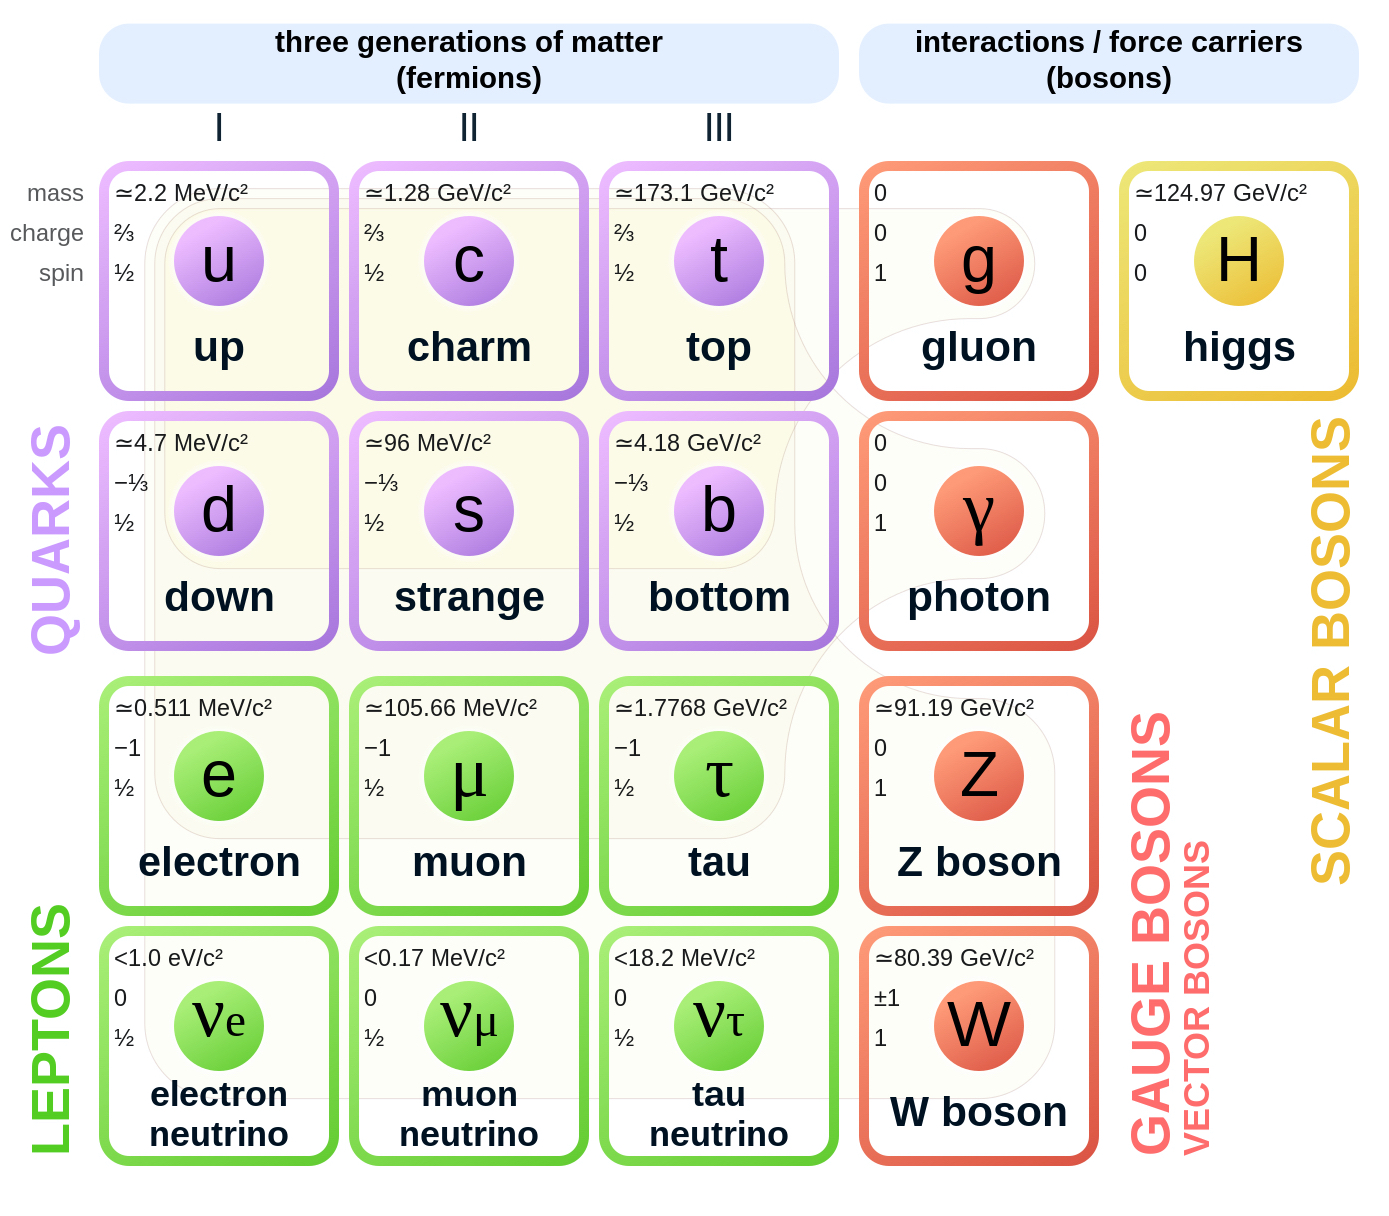
\includegraphics[width=\textwidth]{SM.jpg}
	\vspace{6pt}
	\caption{The elementary particles of the Standard Model. The fermions and bosons are grouped in columns where the quarks, leptons, gauge bosons and scalar Higgs boson are shown in different colours. The three generations of matter are indicated with roman numerals. The mass, charge and spin values corresponding to each particle are indicated on the upper left of each box. The bosons are shown in faint yellow areas with which they interact with.}
	\label{SM-figure}
\end{figure}

Fermions make up the ordinary matter that we see around us everyday. A subgroup of fermions are the leptons and they include electron, muon, tau and their neutrino pairs. Neutrinos have very small mass values compared to other leptons and quarks. They do not have electromagnetic charge which makes them obey only the weak force and they barely interact with matter. Flavours of leptons other than the neutrinos (electrons, muons and taus) have sizeable mass and charge and they are members of the three generations of matter.

The other type of leptons are the quarks. They have three generation as leptons do, and they include six different flavours, namely up, down, charm, strange, top and bottom quarks. They interact with electromagnetic, weak and strong nuclear forces since they have colour charges in addition to their electric charge. 

Bosons are the mediator particles of the three forces described in the SM. The particles of this type are called the gauge boson and they include the photon ($\gamma$), W$^{\pm}$ bosons, Z boson, gluons and the Higgs boson. The photons and gluons do not have mass where W bosons have about 80 GeV/c$^{2}$, Z boson has 91 GeV/c$^{2}$ and the Higgs boson has 125 GeV/c$^{2}$ of mass. Among these, only the W$^{\pm}$ bosons have electric charge, and only the Higgs boson has a spin value of zero making it a scalar boson where all other bosons are spin-1 gauge bosons, meaning that they are vector bosons.

The electromagnetic force, whose quantum field theory is established by the \emph{Quantum Electrodynamics (QED)}, is mediated by photons and acts only on the charged particles.  Almost everything we see in the daily life is thanks to the electromagnetic interactions. The carrier of this force, the photons, do not have the charge of the interaction type, hence do not self-interact. Since the photons have zero mass, their interaction range is unlimited.

The weak interaction, which is responsible for the decay of the particles that is a flavour changing interaction, acts only on the fermions. It has a very short interaction range. The neutral and the charged current interactions are mediated by the vector bosons of the this force, the Z boson and the W$^{\pm}$ bosons, respectively. The Higgs boson in this picture, plays the role of generating the masses of the W$^{\pm}$, and Z bosons through the Higgs mechanism~\cite{Higgs1964, BroutEnglert, Guralnik1964}, and of the quarks and leptons through the Yukawa interaction\cite{Weinberg1967}.

\emph{Quantum Chromodynamics (QCD)} is the theory of the strong interaction and describes the interaction between quarks mediated by the massless gluons. It has an interaction range of about $10^{-15}$ m. Unlike the electromagnetic interaction, the gauge bosons of the strong force possess the charge of the interaction, namely colours, hence can couple to itself. There are 3 types of colour; red, green and blue. Each quark in the universe carry one of these 3 colours - they carry anti-colour if they are anti-quarks - and gluons can be thought of colour carrier particles.

A phenomenon called \emph{the colour confinement} states that colour-charged particles cannot be isolated, meaning that only colour-neutral particles can be observed in nature\footnotemark. This results in that gluons carry a pair of charge consisting a colour and an anti-colour. Also, the hadrons are colour-neutral in two ways; i) with a pair of colour and anti-colour ii) with 3 different types of colour or anti-colour. The first combination makes up mesons, consisting of a quark pair (a quark and an anti-quark) and the second combination forms baryons.

\footnotetext{~Below the Hagedorn temperature ($T_H$) of about 0.15 GeV. At the energies higher than $1.7x10^{12}$ K, hadrons become unstable and it can be thought of the boiling point of the hadronic matter~\cite{Hagedorn2016}.}

Some of the predictions of the SM are observed in the experiments, and there is no other particle or force is found beyond the scope of the SM. However, the SM does not provide answers to the unsolved problems in the fundamental physics such as the non-zero masses of the neutrinos\cite{neutrino-mass}, or the dark matter and the dark energy\cite{PlanckCol} which are the dominated energy content of the universe. Therefore the SM is seen as an effective field theory.

\section{The Standard Model Lagrangian and the Higgs Mechanism}
\label{theSMandHiggs}

The Standard Model describes the mentioned fundamental interactions and elementary particles in a single Lagrangian. It is often considered in two parts: the strong sector offers a description for the particles with colour charges, while the electroweak part consists of the electromagnetism and the weak force. The SM is a renormalised gauge field theory with the $ SU(3)_C \otimes SU(2)_L \otimes U(1)_Y$ gauge form and the charges are colour, weak isospin and hypercharge, respectively. The SU(2)$_L$ and U(1)$_Y$ groups mix and the W$^{\pm}$, Z and $\gamma$ bosons are created where $SU(3)_C$ gauge group describes the strong force. The Lagrangian here, does not involve the particle masses but they are introduced to the theory via \emph{the spontaneous symmetry breaking} of the $SU(2)_L \otimes U(1)_Y$ group, that is the electroweak gauge group, which we will address after studying the SM Lagrangian.

Mathematical interpretation of the SM is provided by \emph{the Quantum Field Theory (QFT)}, where each particle is represented by a quantum field that is pervaded across the space-time. These fields are,
\begin{itemize}
  \item the fermion fields $\psi$,
  \item the electroweak boson fields $W_1$, $W_2$, $W_3$ and B,
  \item the gluon field $G_a$,
  \item the Higgs field $\phi$.
\end{itemize}

The behaviour of the the fundamental fields and the quantum states are determined by the Lagrangian density (usually called \emph{the Lagrangian}). Most of the field theories normally starts with defining a set of symmetries of the system and continues with writing down the renormalisable Lagrangian of the particles or fields that obey these symmetries. The QFT also follows this path; it consists of translational symmetry, rotational symmetry and a boost symmetry that is the invariance of an inertial reference frame. The internal symmetry that defines the SM is a local gauge symmetry of the $ SU(3) \otimes SU(2) \otimes U(1)$ group, where U(1) acts on B and $\phi$, SU(2) acts on W and $\phi$ and SU(3) acts on G fields. The fermion fields also, depending on their charge, transform under these symmetries. The Lagrangian of the SM can be interpreted in three parts; kinetic terms, coupling terms and the mass terms explained by the Higgs mechanism.

\subsection{Kinetic terms}

The kinetic terms, describing the motion of a particle, along with the mass term, represents a free particle. The kinetic term for a fermion field is given by
\be
i\bar\psi\gamma^\mu\psi ,
\ee
where $\gamma^\mu$ denotes the Dirac matrices. In order to find the kinetic terms for the gauge fields, we need to first define the field strength tensor for the spin-1 fields as,
\be
F_{\mu\nu}^a = \partial_\mu A_\nu^a-\partial_\nu A_\mu^a+g f^{abc}A_\mu^b A_\nu^c \hspace{1cm} a,b,c = 1,2,3 ,
\ee
for a given field A with coupling constant g and $f^{abc}$ being the structure constant of the prevailing gauge group defined by the commutator with generators $t_i$;
\be
[t_a,t_b]=if^{abc}t_c .
\ee
Here, we need to bring in three fields that correspond to SM gauge groups.
\begin{itemize}
    \item $B_{\mu}$; the gauge field for the U(1) of weak hypercharge with coupling constant $g\prime$ (or $g_1$) and gauge field tensor $B_{\mu\nu}$,
    \item $W_\mu^a$; the gauge field for the SU(2) group where \emph{a} runs over the three generators of this group. The coupling constant in denoted $g$ or $g_2$ and the gauge field tensor is represented by $W_{\mu\nu}^a$,
    \item $G_\mu^a$; the gluon field of SU(3) where \emph{a} runs over 8 colours. The coupling constant is denoted $g_s$ or $g_3$ and $G_{\mu\nu}^a$ is the gluon field tensor.
\end{itemize}
The kinetic term including all the gauge groups of the SM can be written as,
\be
\Lag_{kin} = -\frac{1}{4g_3^2}\sum_{A=1}^8 G_{\mu\nu}^A G^{\mu\nu A}-\frac{1}{4g_2^2} \sum_{a=1}^3 W_{\mu\nu}^a W^{\mu\nu a}-\frac{1}{4g_1^2} B_{\mu\nu} B^{\mu\nu} ,
\ee
where the structure constants of the U(1) gauge group  cancel out since the generators commute with each other, which is the general case for the Abelian groups. 

\subsection{Coupling terms}

Our approach in this section will be to "couple" the gauge fields to the fermions which leads to the interactions. We can interpret the coupling terms in two parts; the electroweak sector and the quantum chromodynamics sector.

The electroweak sector describes the interaction of the $SU(2)_L\otimes U(1)$ part of the Standard Model's gauge groups. The subscript L of the SU(2) group indicates that the field couples only to the left handed fermions. This is due to the parity-symmetry-violating nature of the weak interaction, which means that the $W^\pm$ bosons are only involved in charged-current interactions of left-handed particles and of right-handed antiparticles. However the $Z$ boson, carrying no electric charge, interacts with both right-handed and left-handed fermion states. In this sense, fermion fields are described with chirality components as left-handed doublets and right-handed singlets. The Lagrangian for the electroweak sector then becomes,
\be
\Lag_{EW} = \sum_\psi\bar\psi\gamma^\mu\left(i\partial_\mu -g_2\frac{1}{2}Y_WB_\mu-g\frac{1}{2}\sigma W_\mu\right)\psi
\ee
where $B_\mu$ and $W_\mu$ are the U(1) and SU(2) gauge fields as defined in \autoref{theSMandHiggs}, $Y_W$ is the weak hypercharge which is the generator of the U(1) gauge group and the components of the $\sigma$ are the Pauli matrices which are the generators of the SU(2) group with the eigenvalues that give the weak isospin values. Here the weak hypercharge symmetry of U(1) is defined different than the Quantum Electrodynamics (QED) in order to unify the electrodynamics with the weak interactions. The relation between the electric charge Q, and the hypercharge $Y_W$ is given by;
\be
Q = T_3 + \frac{1}{2}Y_W
\ee
where $T_3$ is the third component of the weak isospin.

The quantum chromodynamics sector describes the interaction of quarks and gluons, and since the leptons do not carry colour charge, they are not included in this sector. The Dirac Lagrangian of the quark fields coupling to the gluon fields is given by,
\be
\Lag_{QCD} = i\bar U \left(\partial_\mu-ig_3G_\mu^aT^a\right)\gamma^\mu U+i\bar D\left(\partial_\mu-ig_3G_\mu^aT^a\right)\gamma^\mu D ,
\ee
where $T^a$ is the generator of this group and, U and D are the Dirac spinors associated with up-type and down-type quarks, respectively.

\subsection{Higgs mechanism}

So far, we have built the SM on the assumption that the interactions are gauge invariant. This requires the vector bosons $W^\pm$ and $Z$ to be massless. In addition, for a fermion field $\psi$ satisfying the Dirac equation $ (i\hbar\gamma^\mu\partial_\mu-mc)\psi = 0$, the mass term $-m\bar\psi\psi$ arises which is actually not invariant under the SU(2) gauge symmetry. This can be seen by expanding the mass term with left and right handed fermion fields, that is
\be
-m\bar\psi\psi = -m\left(\bar\psi_L\psi_R + \bar\psi_R\psi_L\right) ,
\ee
and have seen that the left-handed fields are doublets under $SU_L(2)$ while right-handed fields are singlet. This means that their gauge quantum numbers are different and this kind of mass term is forbidden. 
The solution to these theoretically massless but experimentally massive particles is given by \emph{the Brout-Englert-Higgs (BEH) Mechanism}~\cite{Higgs1964, BroutEnglert, Guralnik1964}, usually called \emph{the Higgs Mechanism}, showing that the electroweak symmetry can be broken spontaneously under specific conditions. 

The solution starts with introducing a complex scalar field $\phi$ to the theory, which is a doublet under $SU_L(3)$,
\be
 \phi = \frac{1}{\sqrt{2}}
 \begin{pmatrix}
  \phi_1^a+i\phi_2^a \\
  \phi_1^b+i\phi_2^b
 \end{pmatrix} ,
\ee\\
and the Lagrangian describing the Higgs field is given by,
\be
 \Lag_{Higgs} = \left(D_\mu\phi\right)^\dagger\left(D^\mu\phi\right)-V\left(|\phi|^2\right) .
 \label{HiggsLag}
\ee

Since the potential $V$ must satisfy SU(2) and U(1) symmetries, a good solution is a Mexican hat;
\be
 V(\phi) = -\mu^2\phi^\dagger\phi + \lambda\left(\phi^\dagger\phi\right)^2
 \label{higgspotential}
\ee
A spontaneous symmetry breaking (SSB) happens when both the constants $\mu^2$ and $\lambda$ are positive values. A convenient choice for the minimum would be
\be
\langle\phi\rangle=\frac{1}{\sqrt{2}}
 \begin{pmatrix}
  0 \\
  v
 \end{pmatrix} .
\ee
The minimum of this potential is non-zero with the potential shape in \autoref{mexicanHiggs} and given by,
\be
 \begin{aligned}
 \frac{dV}{d\left(\phi^\dagger\phi\right)} &=\mu^2+2\lambda\phi^\dagger\phi = 0 \\
 & \Rightarrow |\phi_{min}| = \sqrt{\frac{\mu^2}{2\lambda}} ,
 \end{aligned}
\ee
which is called \emph{the vacuum expectation value} and measured experimentally and found to be 246 GeV.
\vspace{6pt}
\begin{figure}[ht]
	\centering
	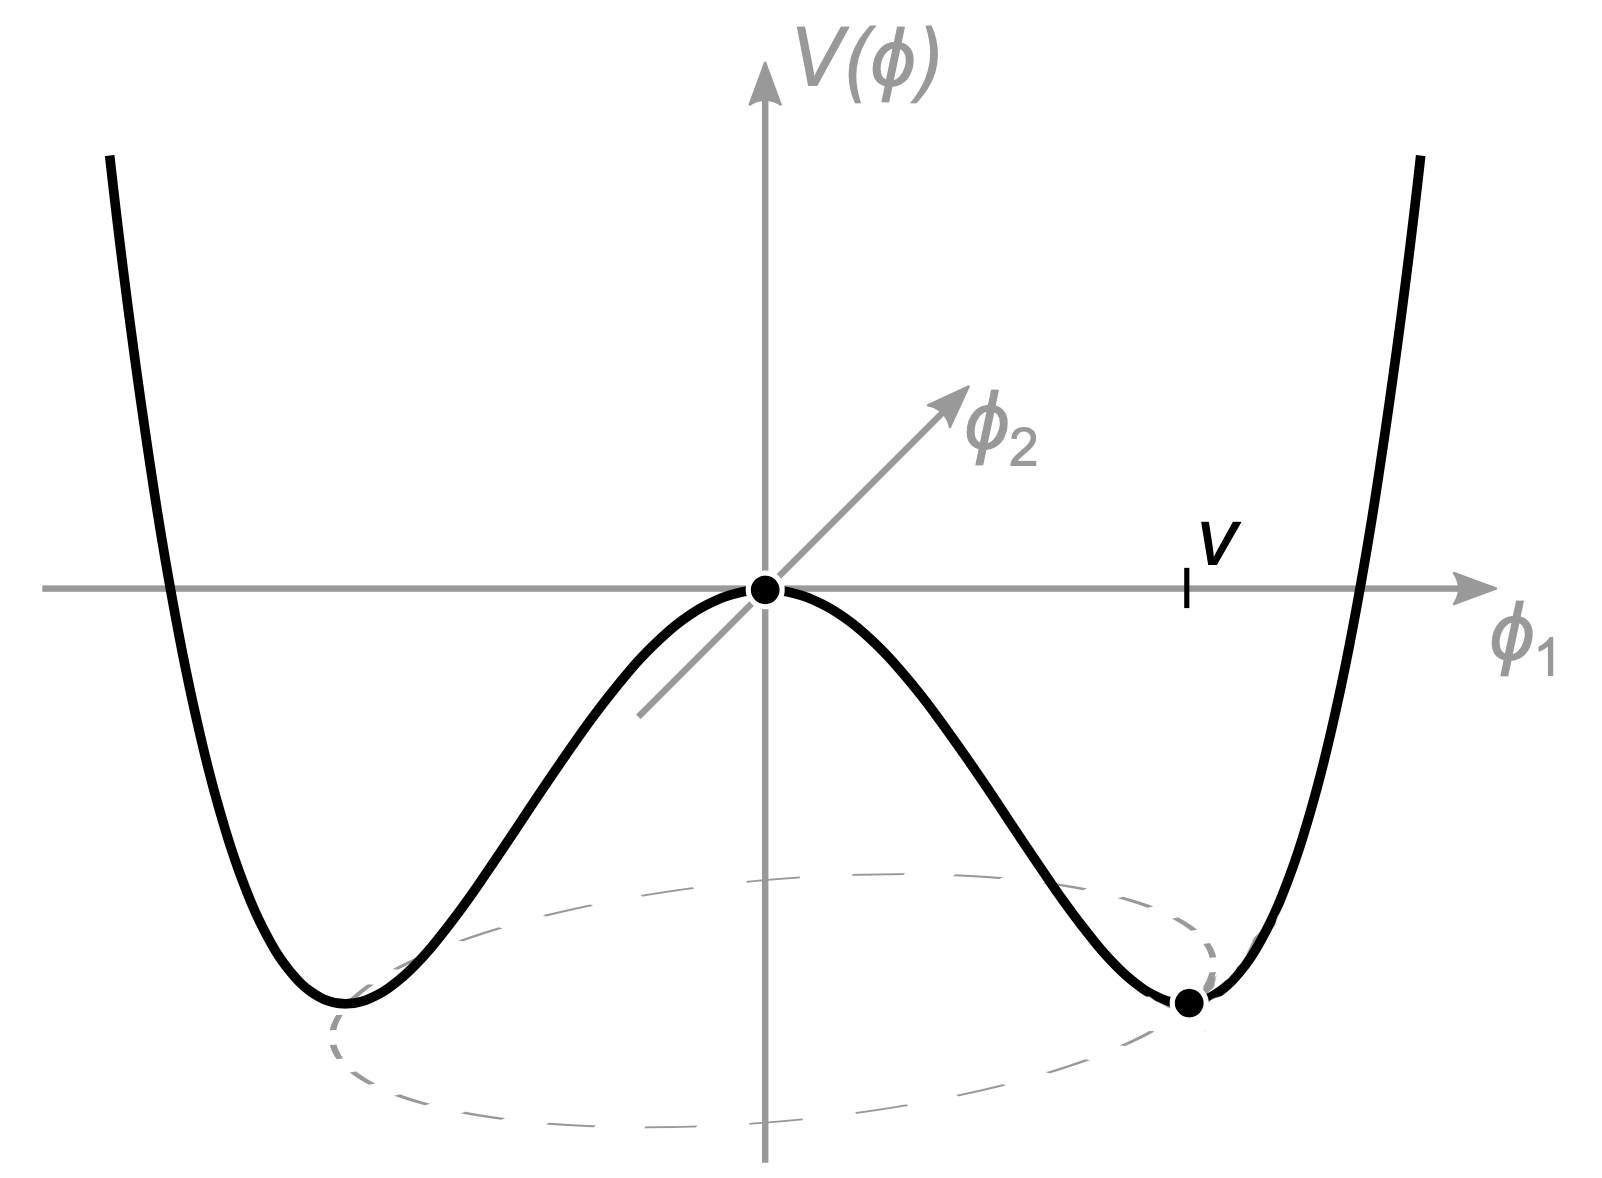
\includegraphics[width=\textwidth]{mexicanhat.png}
	\vspace{6pt}
	\caption{The Higgs potential V in the case that $\mu^2 > 0$. Choosing any point at the bottom of the potential breaks spontaneously the rotational U(1) symmetry.}
	\label{mexicanHiggs}
\end{figure}
Now let us parametrise the complex doublet field $\phi(x)$,
\be
\langle\phi\rangle=\frac{1}{\sqrt{2}}
 \begin{pmatrix}
  0 \\
  v+h(x)
 \end{pmatrix} .
 \label{higgsVparametrized}
\ee
In this case, \autoref{higgspotential} becomes,
\be
V = -\frac{1}{2}m_h^2h^2-\sqrt{\frac{\lambda}{2}}m_hh^3-\frac{1}{4}\lambda h^4 ,
\ee
where $m_h = \sqrt{2\lambda}v$. This potential describes a scalar particle. The first term represents the Higgs mass term while others represent the self interactions of Higgs.
The covariant derivative of the Higgs field is given by,
\be
  D_\mu\phi = 
  \left(\partial_\mu-ig_2A_\mu^a-i\frac{1}{2}g_1B_\mu\right)
  \phi
\ee
and now the vector bosons can be obtained from the gauge bosons as in the followings,
\be
  W_\mu^{\pm}=\frac{1}{\sqrt{2}}\left( A_\mu^1\mp A_\mu^2 \right) ,
\ee
\be
  Z_\mu=cos\theta_WA_\mu^3-sin\theta_WB_\mu ,
\ee
\be
  A_\mu=sin\theta_WA_\mu^3+cos\theta_WB_\mu ,
\ee
where
\be
  sin\theta_W = \frac{g_2}{\sqrt{g_2^2+g_1^2}} ,\; \; cos\theta_W=\frac{g_1}{\sqrt{g_2^2+g_1^2}} .
\ee
\\$\theta_W$ here is called \emph{the weak mixing angle}. Substituting \autoref{higgsVparametrized} with the kinetic term $|D_\mu\phi|^2$ in \autoref{HiggsLag} gives,
\be
\Lag_{kin}=-\frac{1}{2}\left(\partial_\mu\phi\right)^2+\left(m_W^2W^{\mu+}W_{\mu-}+\frac{1}{2}m_Z^2Z^{\mu+}Z_{\mu-}\right)\left(1+\frac{h}{v}\right)^2 ,
\ee
where the mass terms of the massive bosons such as,
\be
m_{W^\pm} = g\frac{v}{2}, \; \; m_Z = \frac{v}{2}
\ee
Leptons, similarly, acquire mass by Yukawa interactions with the Lagrangian,
\be
\Lag_{Yukawa}=-\lambda_l\psi_L\phi\psi_R
\ee
where $\lambda_l$ is the Yukawa coupling to the lepton field $\psi$. After the spontaneous symmetry breaking, the Lagrangian part of the Yukawa coupling to the leptonic field reads,
\be
\Lag_{Yukawa}=-m_f\bar ff\left(1+\frac{h}{v}\right) .
\ee
and leptons acquire mass proportional to their interactions with the Higgs field.

The Higgs boson, required for the spontaneous symmetry breaking, was found experimentally by the CMS and ATLAS experiments at the LHC Experiment at CERN\cite{HiggsCMS,HiggsATLAS} in 2012, almost 50 years after its theoretical assumption. The mass of the Higgs boson is 125 GeV and its parameters; spin, parity and branching ratios are found to be consistent with the Standard Model predictions\cite{Higgsprecision1, Higgsprecision2}.

The most general form of the SM Lagrangian depends on 19 parameters. These parameters are given in \autoref{SMparameters}.
\begin{table*}[h]
	{\setlength{\tabcolsep}{14pt}
		\caption{Parameters of the Standard Model.}
		\begin{center}
			\vspace{-6mm}
			\begin{tabular}{cccc}
				\hline \\[-2.45ex] \hline \\[-2.1ex]
				\# & Symbol & Name & Value \\
				\hline \\[-1.8ex]
				1 & $m_e$ & Electron mass & 0.511 MeV \\
				2 & $m_\mu$ & Muon mass & 105.7 MeV \\
				3 & $m_\tau$ & Tau mass & 1.78 GeV \\
				4 & $m_u$ & Up quark mass & 1.9 MeV \\
				5 & $m_d$ & Down quark mass & 4.4 MeV \\
				6 & $m_s$ & Strange quark mass & 87 MeV \\
				7 & $m_c$ & Charm quark mass & 1.32 GeV \\
				8 & $m_b$ & Bottom quark mass & 4.24 GeV \\
				9 & $m_t$ & Top quark mass & 173.5 GeV \\
				10 & $\theta_{12}$ & CKM 1-2 Mixing angle & 13.1\textdegree \\
				11 & $\theta_{23}$ & CKM 2-3 Mixing angle & 2.4\textdegree \\
				12 & $\theta_{13}$ & CKM 1-3 Mixing angle & 0.2\textdegree \\
				13 & $\delta$ & CKM CP violation Phase & 0.995 \\
				14 & $g_1$ or $g\prime$ & U(1) gauge coupling & 0.357 \\
				15 & $g_2$ or g & SU(2) gauge coupling & 0.652 \\
				16 & $g_3$ or $g_s$ & SU(3) gauge coupling & 1.221 \\
				17 & $\theta_{QCD}$ & QCD vacuum angle & $\sim $ 0 \\
				18 & $v$ & Higgs vacuum expectation value & 246 GeV \\
				19 & $m_H$ & Higgs mass & 125 GeV \\
				\hline
			\end{tabular}
			\vspace{-6mm}
		\end{center}
		\label{SMparameters}}
\end{table*}

\section{Higgs Boson and Tau Leptons}

\section{BSM Searches}

                                       
%\chapter{THE LHC AND THE CMS EXPERIMENT}\label{Ch2}

European Organisation for Nuclear Research, best know as CERN, is established in 1954 by 12 European countries and is based at the Franco-Swiss border in northwest Geneva, Switzerland. Today, the organisation operates the largest particle physics laboratory in the world and has 23 member states \cite{CERN:2771424} and many others that make up more than 11 thousand researches and more than 70 countries around the globe. CERN's main activity is to provide the particle accelerators and needed infrastructure for high energy physics research. The organisation hosts the LHC Experiment which is the world's largest particle collider.

This chapter introduces the structure and operations of the LHC and the CMS Detector on which the simulated Monte Carlo event samples are based in this thesis.

\section{The Large Hadron Collider}

The Large Hadron Collider consists of a 27-kilometre ring tunnel where the beams of particles (protons or lead ions) are accelerated with the help of superconducting magnets along with a number of accelerating systems. It was built between 1998 and 2008 and it lies 175 metres beneath the surface with a total cost of the project expected to be of the order of 4.4\$ billion. The initial design of the LHC aimed at the centre-of-mass energy of $\sqrt{s}=14$ TeV with a nominal peak luminosity of $\mathcal{L} = 10^{34}cm^{-2}s^{-1}$ \cite{Baconnier:257706}. The LHC collides proton-proton beams as well as lead-lead (Pb - Pb), proton-lead (p - PB) and Xenon-Xenon (Xe - Xe) nuclei to study heavy-ion collisions. The \textbf{\emph{LHC accelerator complex}} consist of a series of accelerators and is used to accelerate protons before being injected in the LHC, which will be explained shortly.

\subsection{Operation of the LHC}

The success of the LHC required two decade-long international collaboration. The initial studies started in the early 1980s when the The Large Electron Positron Collider (LEP) at CERN was not even running. CERN Council approved the construction of the LHC in 1994 and a technical design report was published the next year. Starting from 1998, the construction of the LHC was completed in 2008 and it succeeded to accelerate proton beams the same year \cite{lhcfirstbeams}. The first accelerated proton beams had an energy of 450 GeV per beam and later on the collisions at $\sqrt{s}=2.14$ TeV with respect to Tevatron at 1.96 TeV and made the LHC the highest-energy collider ever built. In 2010, LHC increased the beam energy to 3.5 TeV which was a world record of man-made particle acceleration.

Data collection started in 2010 and finished in 2013; this time period is known as Run I of the LHC. The CMS Experiment collected about 45$pb^{-1}$, 6 $fb^{-1}$ and 23 $fb^{-1}$ data at $\sqrt{s}=7$ TeV in 2010, 2011 and 2012, respectively. The data collected at Run I has lead the discovery of the Higgs boson. LHC entered an upgrade stage called Long Shutdown 1 (LS1) for two years when Run I is finished in 2012. LHC was upgraded in LS1 in the way of achieving its design performances, and started its operation again in 2015 for a period of 3 years known as Run II but his time the beam energy was 6.5 TeV. The Run II is finished in 2018 with a data amounting to about 150 $fb^{-1}$ and LHC entered LS2 with a schedule to be in Run III in 2022 at $\sqrt{s}=14$ TeV. The LS3 is planned to be the update period where the LHC will have an unprecedented instantaneous luminosity corresponding to an integrated luminosity of 3000 to 4000 $fb^{-1}$ eventually, called the High-Luminosity LHC (HL-LHC) or Phase II. Both the LHC and the HL-LHC plans shown in \autoref{HLLHCplan}.

\begin{figure}[ht]
	\centering
	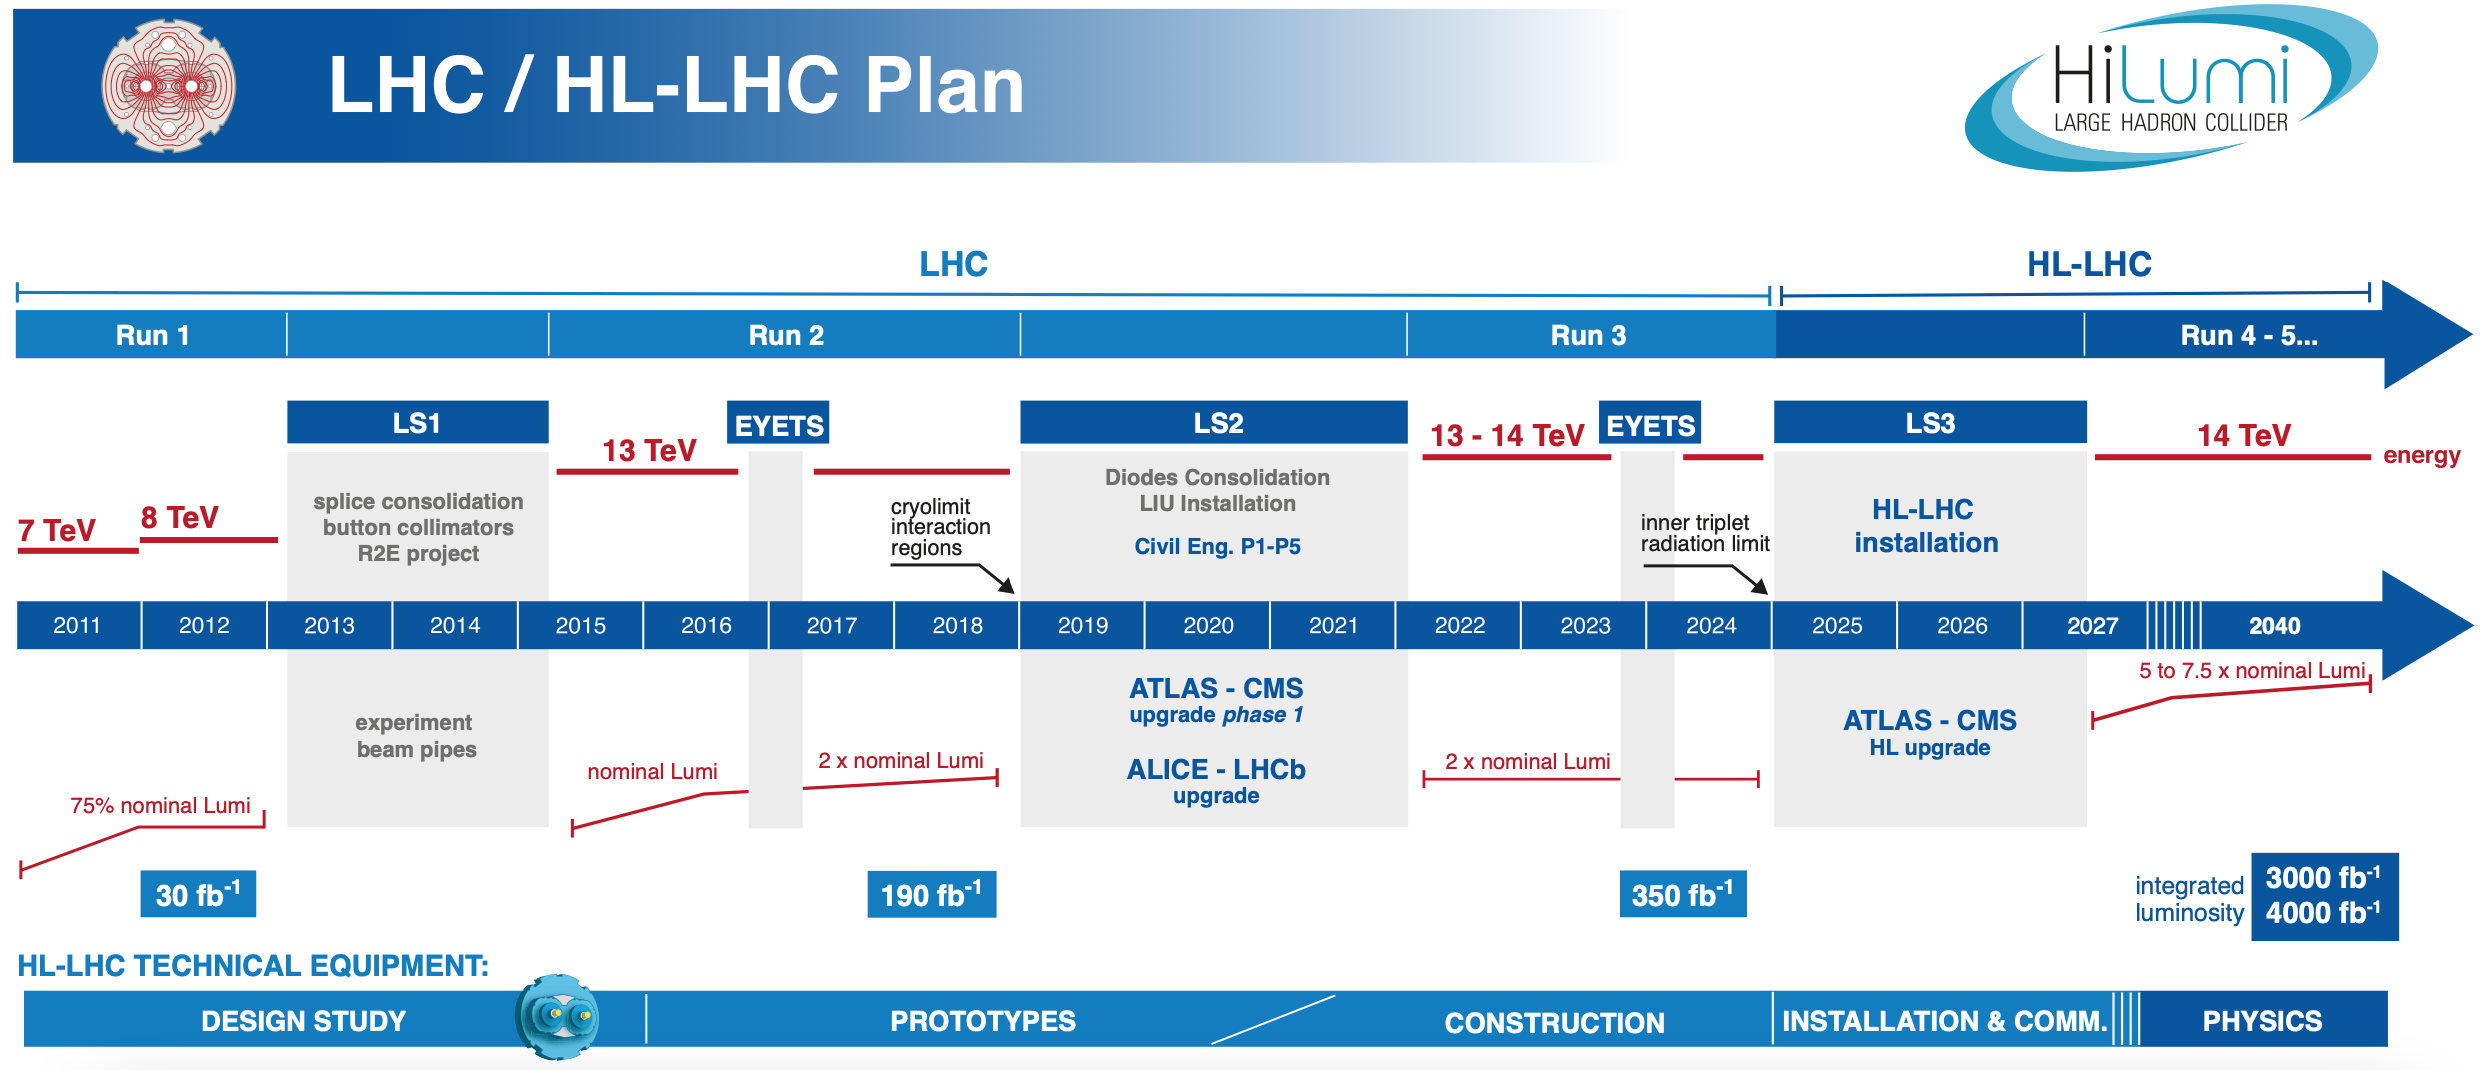
\includegraphics[width=\textwidth]{MSc_Thesis/fig/HLLHCplan.png}
	\vspace{2mm}
	\caption[A detailed schedule of LHC and HL-LHC showing the integrated luminosity and the beam energy corresponding to each period.]
	{A detailed schedule of LHC and HL-LHC showing the integrated luminosity and the beam energy corresponding to each period \cite{Apollinari:2284929}.}
	\label{HLLHCplan}
\end{figure}

The main scope of the HL-LHC is to increase the collision data which will allow physics searches to be more statistically abundant and be able to perform higher-precision measurements.

\subsection{The Accelerator Complex}

The accelerator tunnel of the LHC, which was previously used host LEP collider, has two parallel vacuum pipes where two counter-rotating beams are kept inside a magnetic field generated by superconducting niobium-titanium (NbTi) cables. The magnetic field generated to steer the beams are about 8 Tesla which is more than 100 000 times higher than the Earth2s magnetic field. This field is generated by  1232 dipole magnets each with a 14 metres of length and 35 tonnes of weight where 11 thousand Ampers of electric current flows. This acceleration system allow the beams to circulate with 7 TeV energy. The focusing of the beams in a narrow area is secured by 392 quadrupole magnets with 5 to 7 m lengths. In order to inject the beams in the collision points, special quadrupoles are positioned at each entrance to squeeze the beams in a narrower area. These superconducting magnets are cooled down to a temperature of 1.9 K by a cyrogenics cooling system supplied with 120 tonnes of Helium-4 fluid.

Before being injected into the LHC, the proton beams are pulled off from hydrogen gas and accelerated by a series of systems gradually increasing their energy, presented in \autoref{LHCacc}. Firstly, protons are accelerated to an energy of 50 MeV in the Linear Accelerator (LINAC2) then injected into the Proton Synchrotron Booster (PSB) where beams are re-accelerated to 1.4 GeV. These particles are sent to the Super Proton Synchrotron (SPS) to further accelerate them to 450 GeV energy. The final injection is made from the SPS to LHC's two beam pipes in the counter directions. The filling of the LHC by protons takes about 8 minutes, and 20 minutes for protons to be accelerated to 6.5 TeV of energy in bunches via Radio Frequency (RF) cavities operating. The injected beams circulate the LHC rings for many hours (12 hours) under normal operation. The bunches are spaced by 25 ns or 7.5 metres thus the bunch crossing rate is 40 MHz. Nominal number of protons per bunch is $12x10^{11}$ and the nominal number of bunches per beam is 2808 contributing to an inelastic collision event in the order of $10^9$ per second with about 20 collisions per bunch crossing.

\begin{figure}[ht]
	\centering
	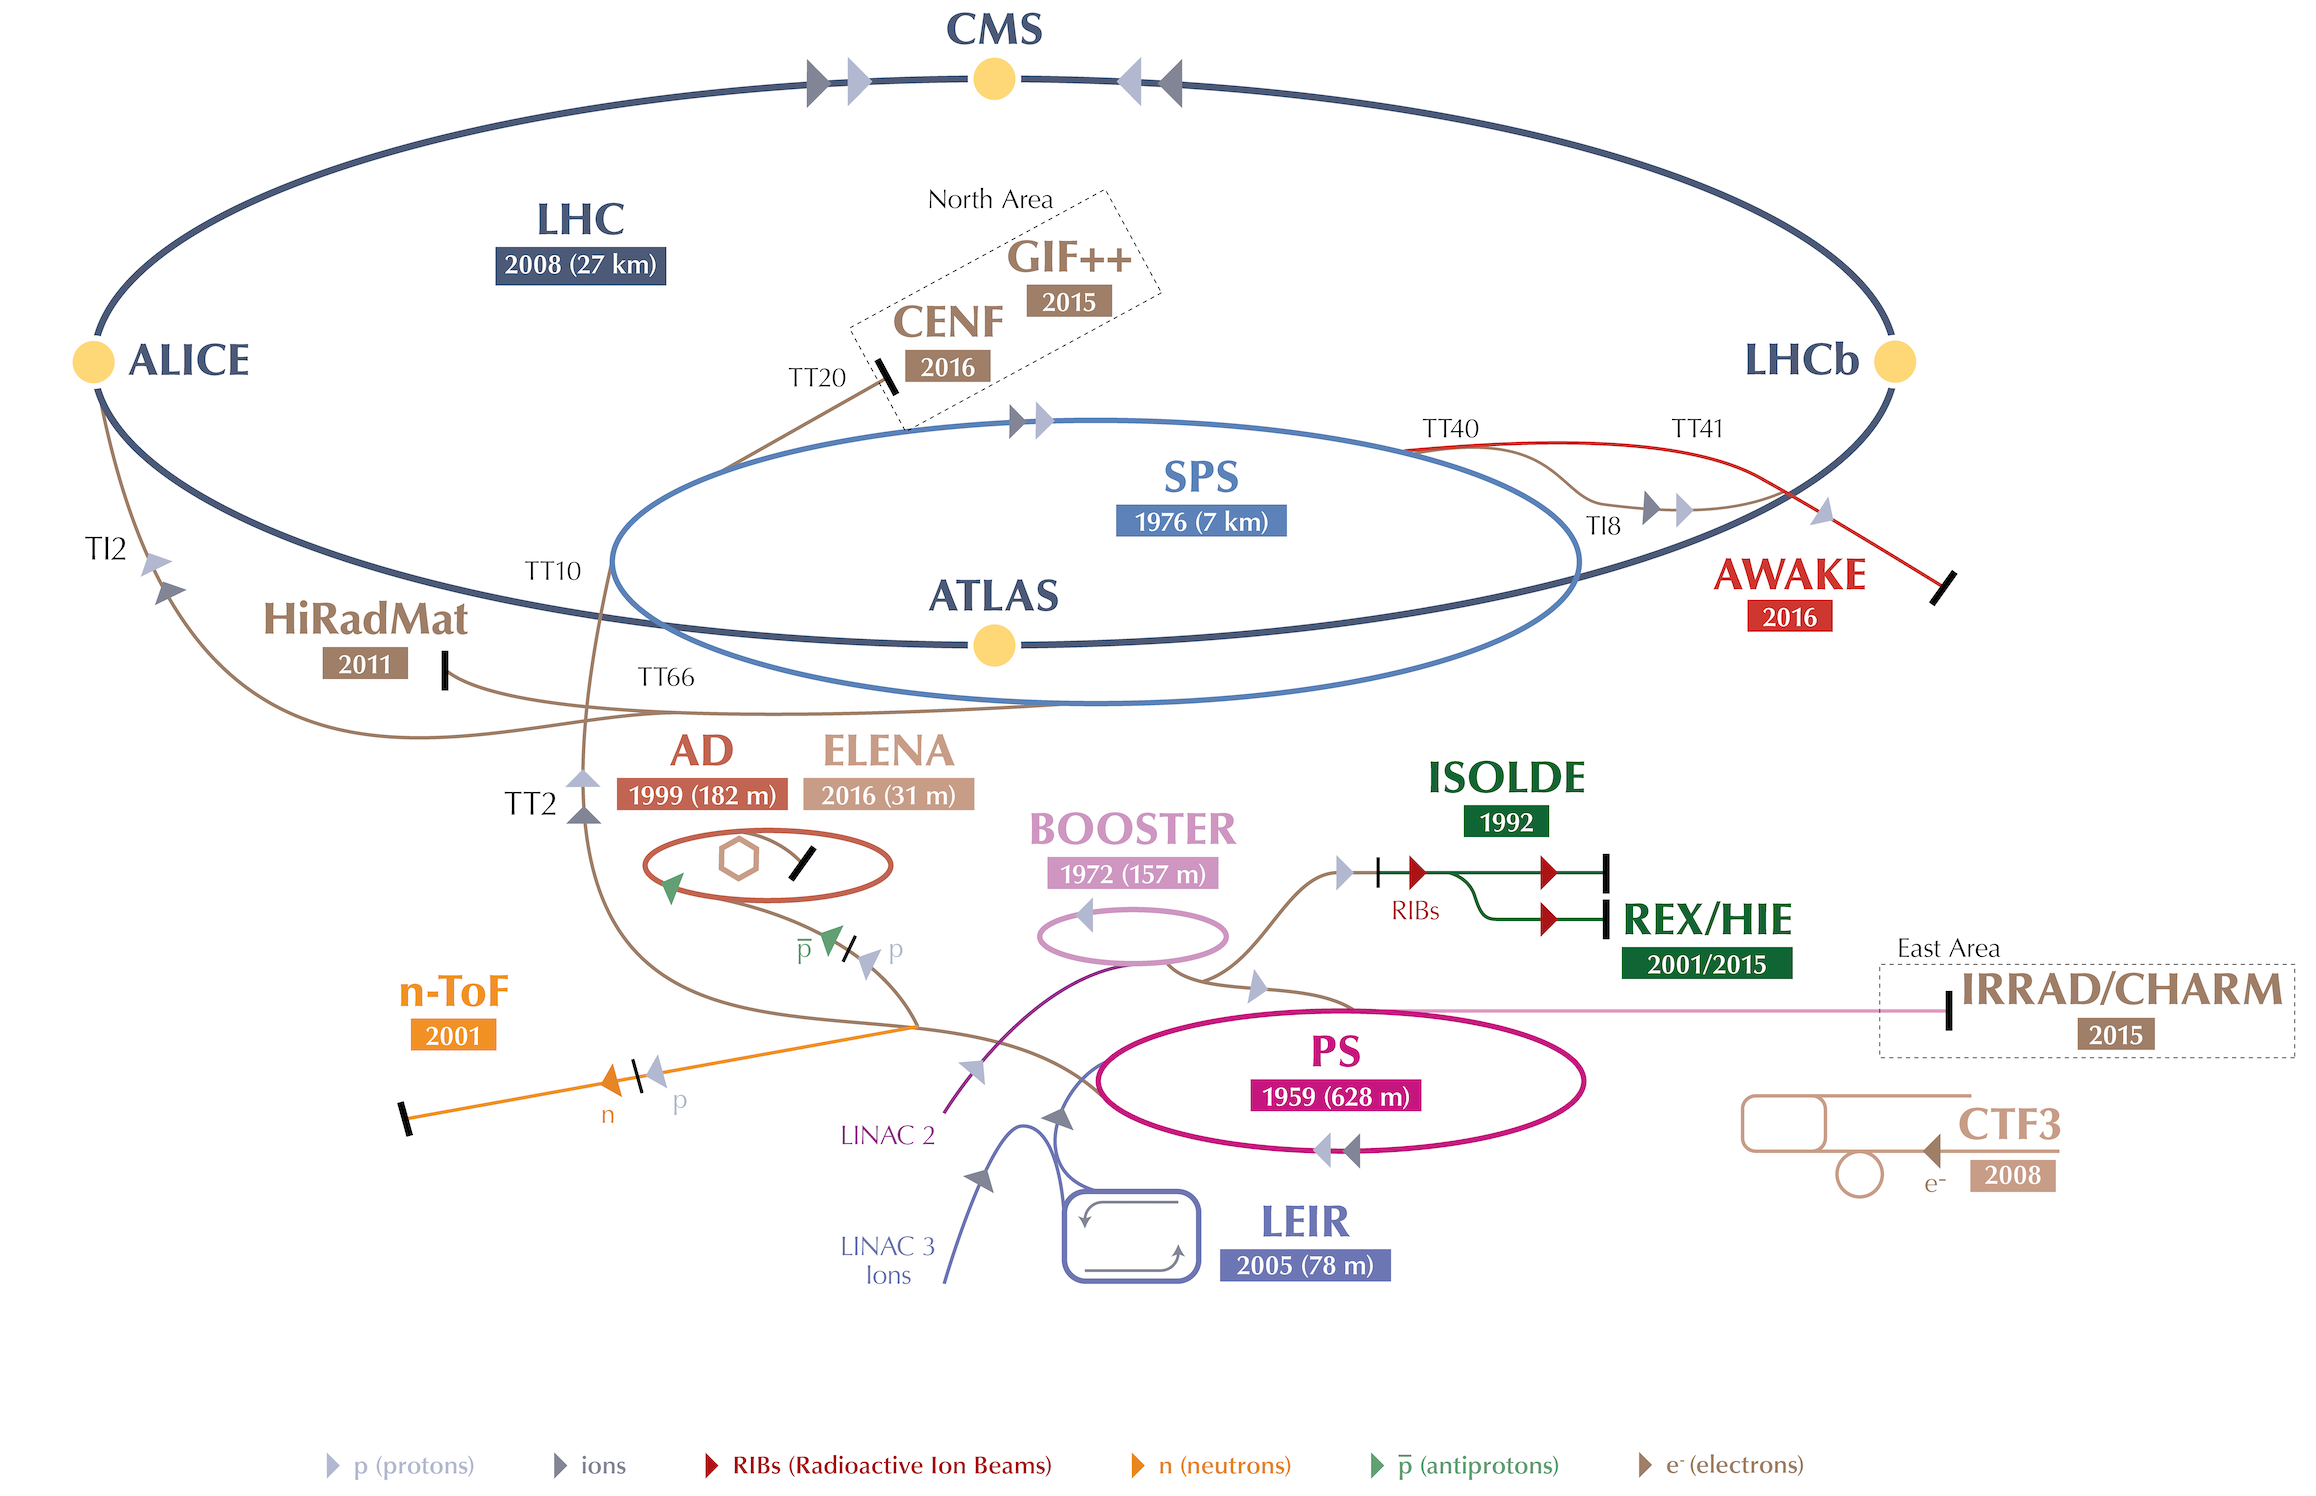
\includegraphics[width=\textwidth]{MSc_Thesis/fig/LHCacc.png}
	\vspace{2mm}
	\caption[The LHC accelerator complex. The acceleration of the protons start in the LINAC2 and ends in LHC through Booster, PS and SPS.]
	{The LHC accelerator complex. The acceleration of the protons start in the LINAC2 and ends in LHC through Booster, PS and SPS \cite{Mobs:2197559}.}
	\label{LHCacc}
\end{figure}

The accelerated beams of particles are collided inside one of the four detectors; ALICE, ATLAS, CMS and LHCb. The ATLAS and CMS Detectors are installed in opposite sides, at Point 1 and Point 5 of the LHC. These two detectors are designed as multi-purpose detectors that surround the collision points to detect any out-coming particle. They are described in detail in the references \cite{ATLAS2008, CMS2008}. ALICE Experiment is installed at Point 2 and its main purpose is to study heavy ion collisions and quark-gluon plasmas. Final of the four large experiments, LHCb, located at Point 8, is a forward one sided detector mainly aimed at measuring the charge conjugation and parity symmetry violation in Beauty baryons. The detailed description of the two detectors can be found in \cite{ALICE2008, LHCb2008}.

LHC host many other experiments; the LHCf \cite{LHCF2006} and TOTEM \cite{TOTEM2004} Experiments positioned at 100 meters away from the both sides of the ATLAS and CMS's collision points. These experiment study mainly the pp interactions and forward physics. Others are the MoEDAL\cite{moedal} Experiment which is dedicated to search for magnetic monopoles at the same experimental cavern with LHCb detector, and the FASER Experiment searching for lighter particles and studying neutrinos situated 480 metres away from the ATLAS's collision point.

\subsection{Design and specifications}

The \textbf{\emph{collision energy}} of the particles inside the detectors is one of the most important parameters at the LHC and is simply the sum of the energy of two colliding beams. When these collisions happen, independent types of interactions may happen between protons. The \textbf{\emph{soft interactions}} signify a small amount of transferred momentum which means the interacting protons barely came close to each other and escapes without decaying at all. The \textbf{\emph{hard interactions}} on the other hand, signify a high transferred momentum which causes the proton to decay. When two protons collide, a fraction of the energy ($s\prime$) contributes to the interaction since it is actually the partons of the protons that participate in the collision proportional to the fraction of energies ($x_1,\; x_2$) of each parton.
\be
\sqrt{s\prime} = \sqrt{x_1 x_2 s}
\ee
Another important parameter is the \textbf{\emph{instantaneous luminosity}} for the LHC apparatus. It is a description of the number of collisions per time and cross section. It is given by the following formula,
\be
L = \frac{N_b^2 n_b f_{rev} \gamma}{4 \pi \epsilon_n \beta}F \; ,
\ee
where $N_b$ is the number of particles in each bunches of $n_b$ bunches circulating in the accelerator ring with $f_{rev}$ frequency. The parameters $\gamma$, $\epsilon_n$, $\beta$ and the factor $F$ denotes the relativistic Lorentz factor; emittence and focal length describing the shape and focus of the beam, and geometrical reduction which depends on the angle between two beams, respectively. The luminosity lifetime $\tau$ on the other hand shows how luminosity decreases with time,
\be
L = L_0 e^{-t/\tau} \; ,
\ee
where $L_0$ is the peak luminosity at time zero.

The integrated luminosity, which is another important parameter, is given by $L = \int L dt$ and takes part in the total amount of collisions over time.
\be
N = L x \sigma
\ee
is the number of events produced for a particular physics process with the cross section $\sigma$. Thus, in order for a rare process to be observed in the detectors, maximising the luminosity is essential. In \autoref{SMcrosssections}, the cross sections as a function of $\sqrt{s}$ is shown. It is obvious that the Higgs processes are several orders of magnitude lower in production cross section than the dominant processes, however since the cross section increases with the increasing centre-pf-mass energy, it is necessary to increase also luminosity and $\sqrt{s}$ in order to achieve higher event rates. The integrated luminosity delivered to the CMS experiment since 2010 is shown in \autoref{CMSlumi}.
\begin{figure}[ht]
	\centering
	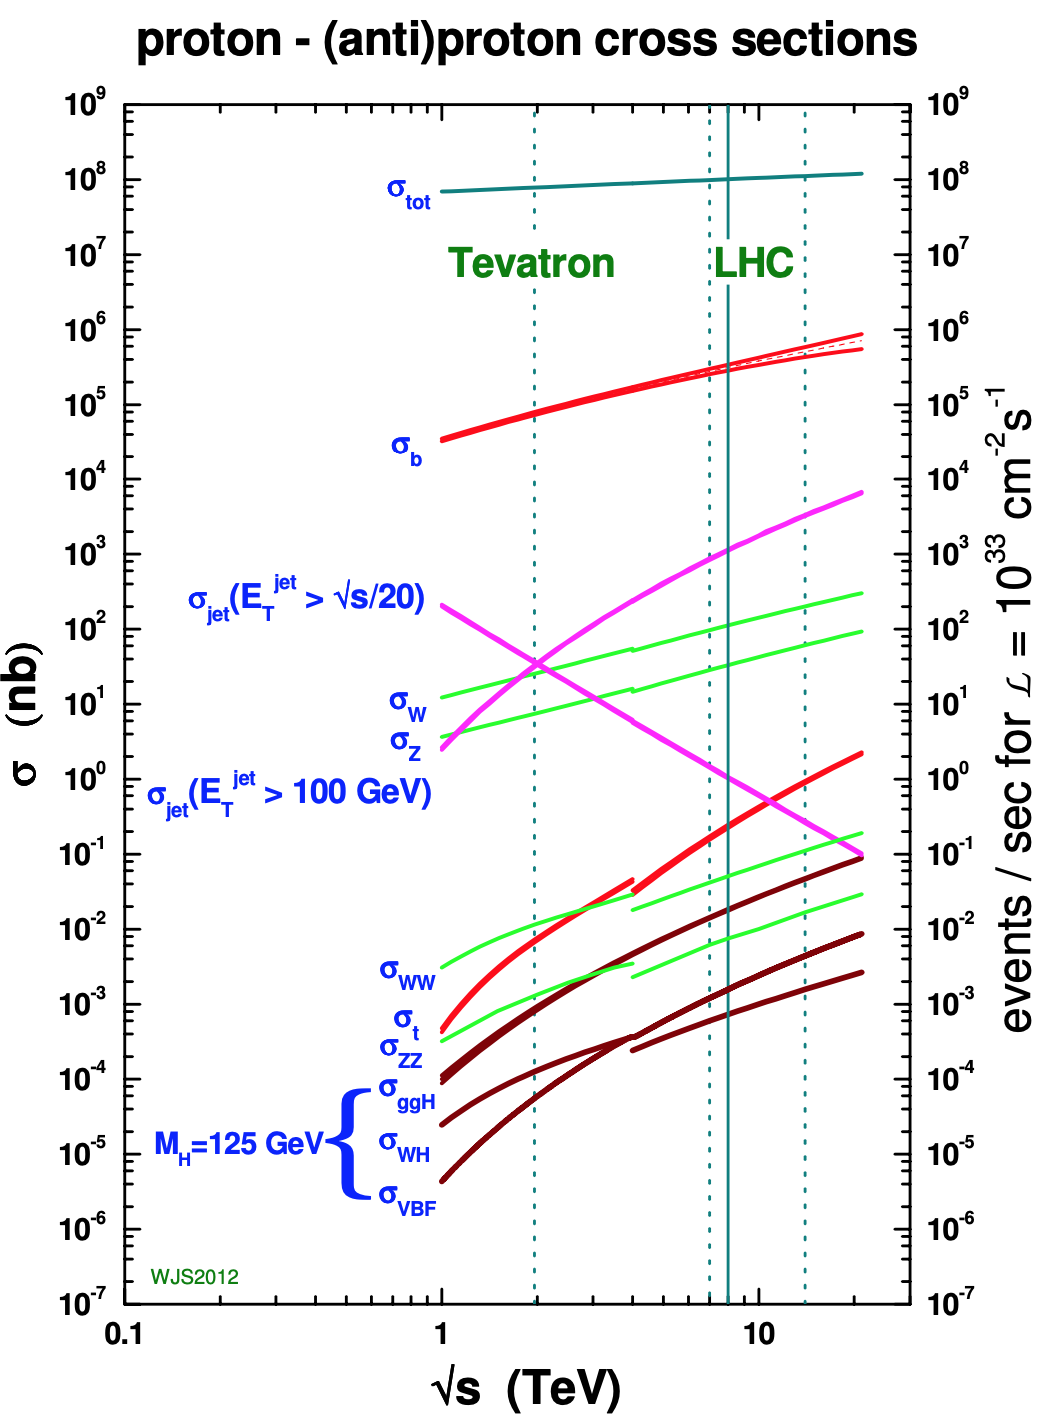
\includegraphics[scale=0.5]{MSc_Thesis/fig/stirling.png}
	\vspace{2mm}
	\caption[Cross sections of Standard Model processes as function of collider energy at pp collisions.]
	{Cross sections of Standard Model processes as function of collider energy at pp collisions\cite{stirling}.}
	\label{SMcrosssections}
\end{figure}

The large instantaneous luminosity of the LHC causes a disadvantage. Multiple pp collisions happen at each bunch crossing and many primary vertices are superimposed. Most of these parton interactions have relatively small centre-of-mass energy, hence they are not of much interest for the experiment, which is often called \textbf{\emph{in-time pileup (PU)}} interactions. Therefore, the detector needs to resolve these pileup interactions from the hard collisions. Besides, since the collisions take place at the heart of the CMS detector, it is inevitable that new particles reach the detector before the products of the previous bunch crossing escapes the detector. This type of pile up is called \textbf{\emph{out-of-time pileup}} interactions. In order to overcome these demanding conditions, highly granular and fast-response detectors are needed. Moreover, the detector needs to be resistant to radiation as well as be precise in energy measurements. The Compact Muon Solenoid, an appropriate detector designed to overcome these challenges, is explained in the next section.

\begin{figure}[ht]
	\centering
	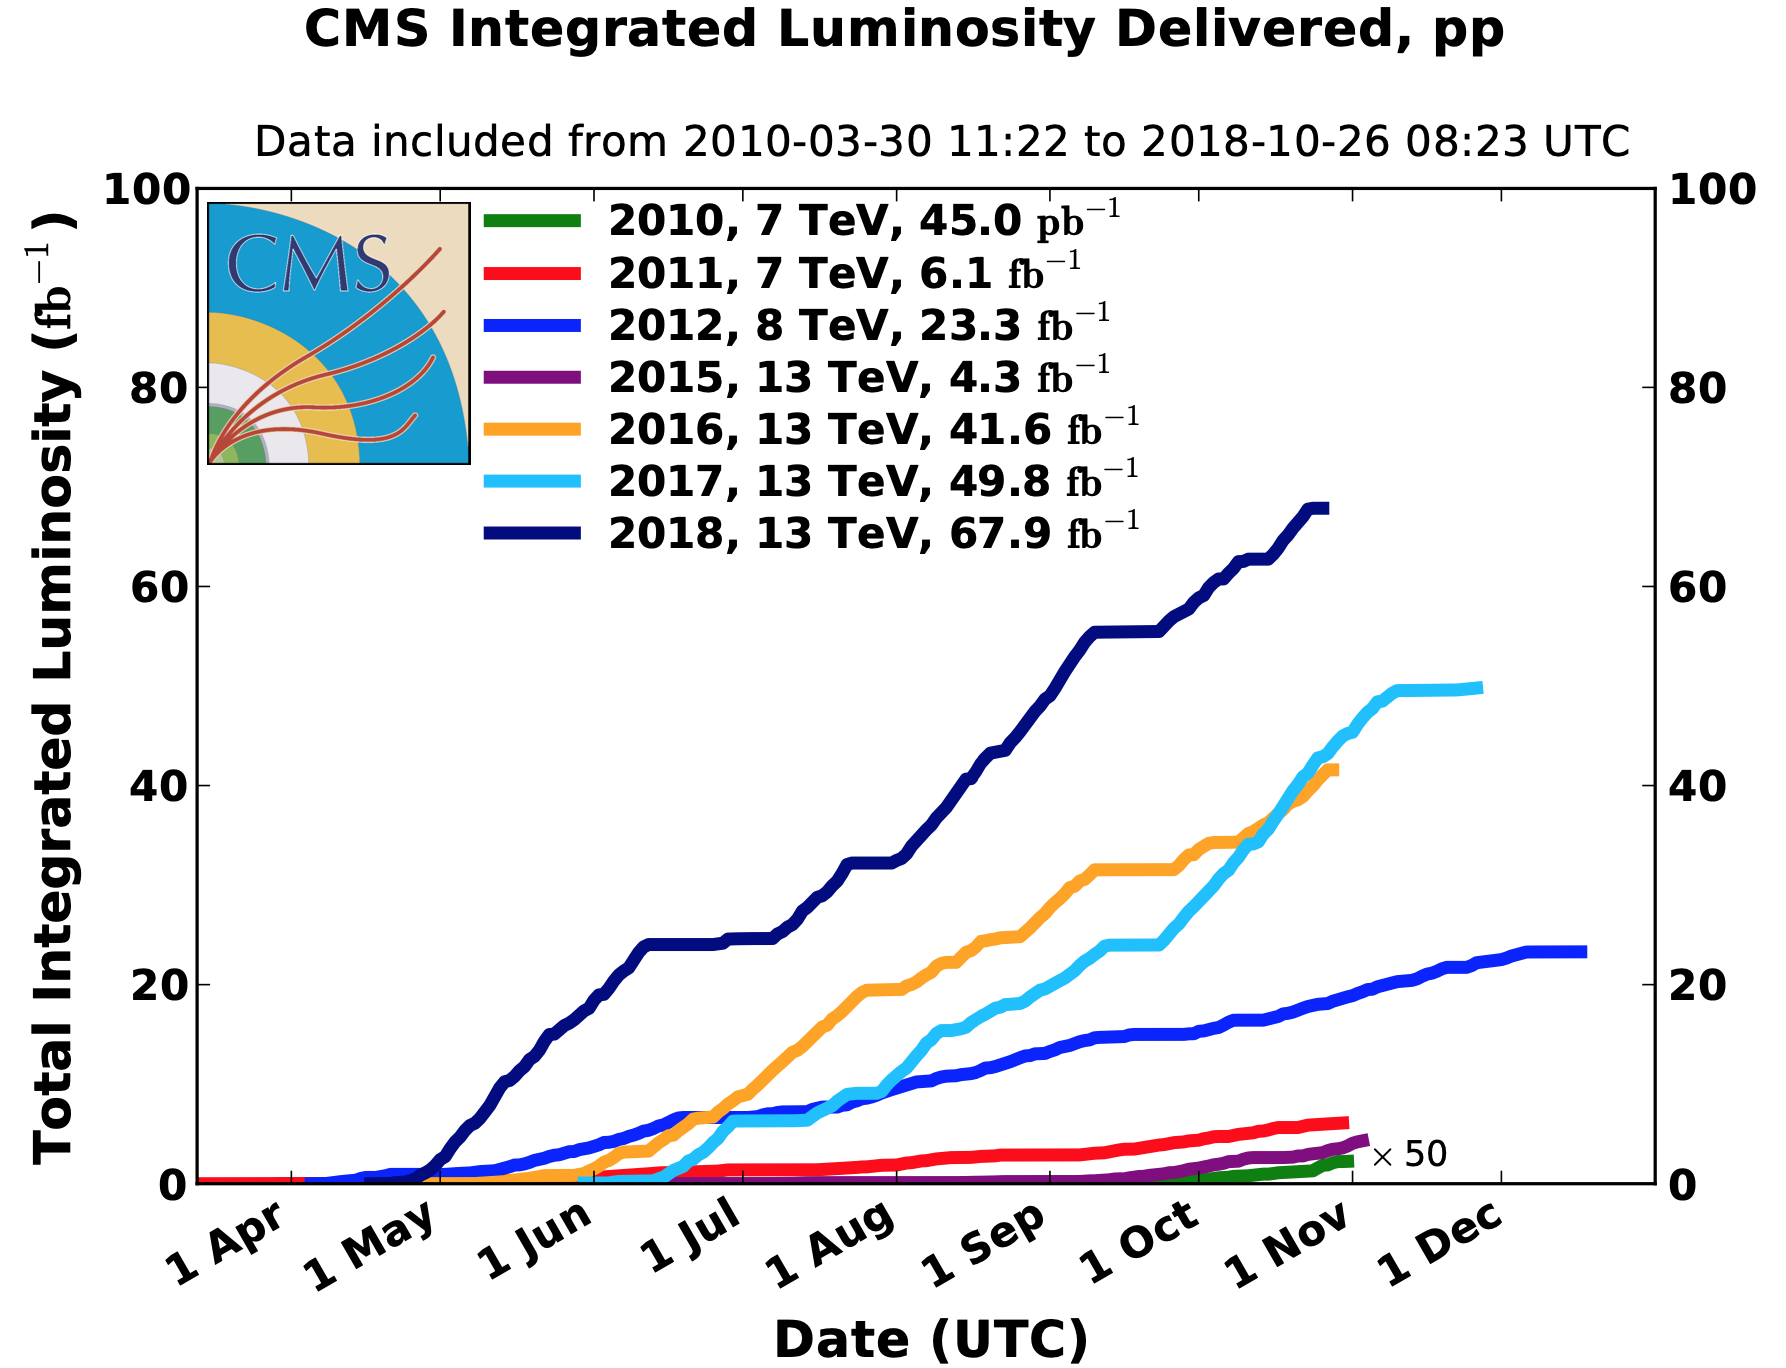
\includegraphics[scale=0.4]{MSc_Thesis/fig/CMSlumi.png}
	\vspace{2mm}
	\caption[Total integrated luminosity delivered by the LHC to the CMS detector for pp collisions at Run I-II.]
	{Total integrated luminosity delivered by the LHC to the CMS detector for pp collisions at Run I-II \cite{CMSlumi}.}
	\label{CMSlumi}
\end{figure}












%%%%%%%%%%%%%%%%%%%%%%%%%%%%%%%%%%%%%%%%%%%%%%%%%%%%%%%%%%%%%%%%%
\chapter{ANALYSIS}\label{ch:Ch3}
%%%%%%%%%%%%%%%%%%%%%%%%%%%%%%%%%%%%%%%%%%%%%%%%%%%%%%%%%%%%%%%%%
\vspace*{-12pt} % If no text above section, use this vspacing to lift the whole part to the proper starting point - SBÖ

\section{Strategy}

\section{Event Samples}

\subsection{Monte Carlo Event Generation}

\subsection{Signal and Background Samples}

\subsection{The Phase-II CMS Detector Response}

\section{Objects}

\subsection{Photons}

\subsection{Leptons}

\subsection{Jets}

\subsection{Missing $E_{T}$}

\section{Event Selection and Categorization}

\subsection{Bamboo Framework}

\subsection{Baseline Selection}

Bamboo Framework to be explained in detail here.

\subsection{Machine Learning Employment}

\section{Systematic Uncertainties}


\chapter{RESULTS \& CONCLUSION}\label{ch4}

Results are performed by fitting the invariant mass distributions of the two leading and sub-leading photons using a binned maximum likelihood approach. The full systematic uncertainties are also applied in the form of nuisance parameters with log-normal distributions. These steps are performed with \textsc{Higgs Combine Tool} \cite{CMS-NOTE-2011-005}. The correlations among different sources of systematic uncertainties are taken into account while different final states are considered as independent in the fit. The significance values obtained are shown in \autoref{wwsigmas} for \wwgg final states and in \autoref{ttsigmas} for \ttgg final states. A combination of all the two channels are shown in \autoref{allsigmas}. A 0.277 $\sigma$ is reported in the combination of the \wwgg and \ttgg final states of double Higgs production. Fitted distributions for the best DNN categories of semi-leptonic \wwgg channel and for the single $\tau$ DNN categories are shown in \autoref{fits} while all final state fit distributions are given in \autoref{allfits}.

\begin{table}[h]
    \centering
    \caption{Significance numbers extracted in each category of one lepton final state, two leptonic final state and their combination.}
    \begin{tabular}{lccc}
    \hline
      \hline 
      Categories & Significance & Significance & Significance \\
       & (stat) & (stat+exp) & (stat+exp+theory)\\
       \hline
      Category 1 & 0.0150 & 0.0138 & 0.0138 \\ 
      Category 2 &0.0555 & 0.0532 & 0.0530 \\ 
      Category 3 & 0.1256 & 0.1215 & 0.1210 \\ 
      Category 4 & 0.2320 & 0.2275 & 0.2267 \\ 
      \hline
      Semi-leptonic combined & 0.2700 & 0.2586 & 0.2567 \\
      \hline
      Fully-leptonic & 0.0955 & 0.0953 & 0.0952 \\
      \hline
      \hline
      \wwgg combined & 0.2864 & 0.2743 & 0.2721 \\ 
      \hline
      \hline
    \end{tabular}
    \label{wwsigmas}
\end{table}
  
\begin{table}[h!]
  \centering
  \caption{Significance numbers extracted in each category of one tau final state, two tau's final state and their combination.}
  \begin{tabular}{lccc}
  \hline
      \hline 
      Categories & Significance & Significance & Significance \\
       & (stat) & (stat+exp) & (stat+exp+theory)\\
       \hline
    Category 1 & 0.0120 & 0.0111 & 0.0110 \\ 
    Category 2 &0.0551 & 0.0537 & 0.0536 \\ 
    \hline
    1 $\tau$ & 0.0564 & 0.0552 & 0.0551 \\ 
    \hline
    2 $\tau$s & 0.0363 & 0.0360 & 0.0358 \\ 
    \hline
    \hline
    Combination & 0.0671 & 0.0655 & 0.0652 \\ 
    \hline
    \hline
  \end{tabular}
\label{ttsigmas}
\end{table}

\begin{table}[h!]
    \centering
    \caption{
    Full Phase-II results of WW$\gamma\gamma$ and \ttgg processes with combination.
    }
  \begin{tabular}{lccc}
  \hline
      \hline 
      Categories & Significance & Significance & Significance \\
       & (stat) & (stat+exp) & (stat+exp+theory)\\
       \hline
    \wwgg & 0.2864 & 0.2743 & 0.2721 \\ 
    \ttgg & 0.0671 & 0.0655 & 0.0652 \\ 
    \hline
    \hline
    Combination & 0.2942 & 0.2795 & 0.2770 \\
    \hline
    \hline
  \end{tabular}
    \label{allsigmas}
\end{table}

\begin{figure*}[h!]
    \centering
    \begin{subfigure}[b]{0.475\textwidth}
        \centering
        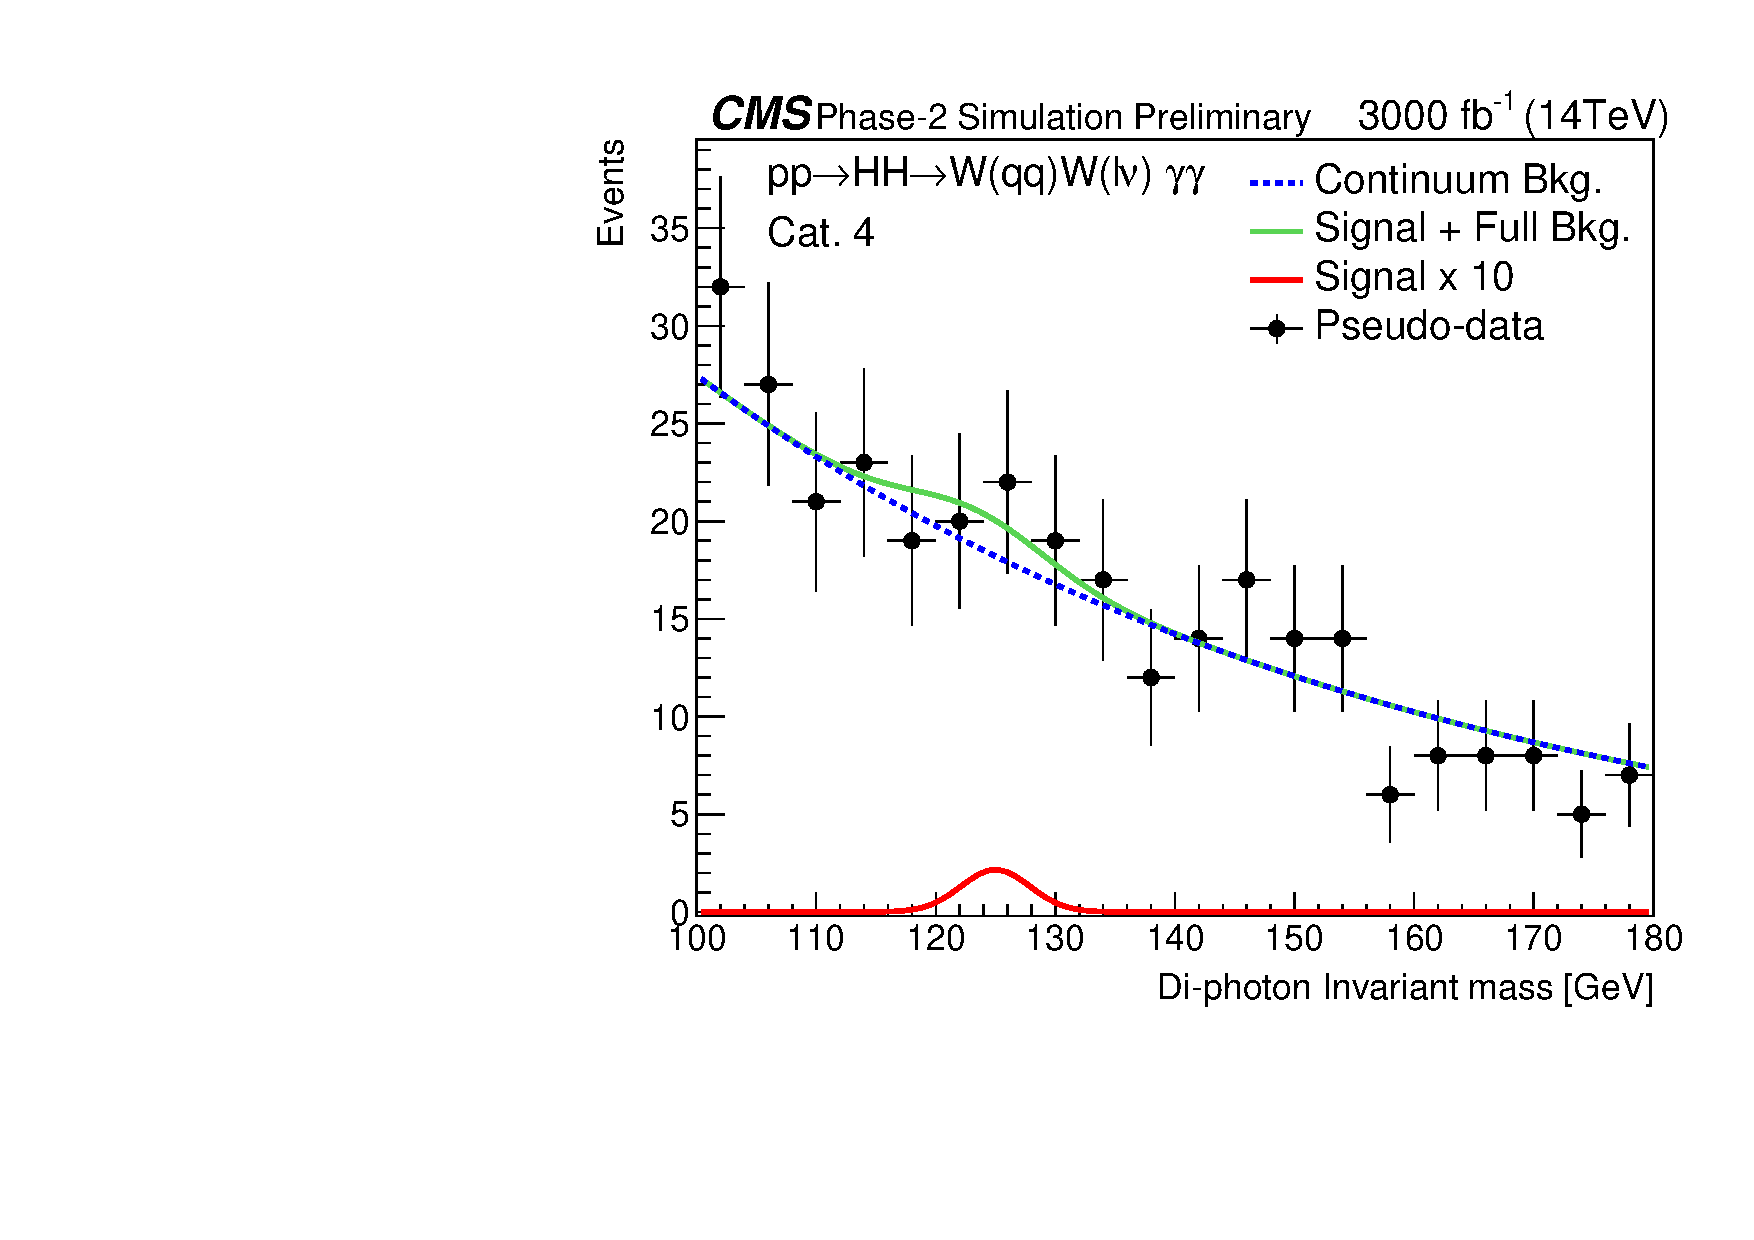
\includegraphics[width=\textwidth]{Inv_mass_gghasOneL_DNN_4_HL_FIT.pdf}
        \vspace{0.1cm}
        %\firstsubcaption{No selection}
    \end{subfigure}
    \hspace{0.2cm}
    \begin{subfigure}[b]{0.475\textwidth}  
        \centering 
        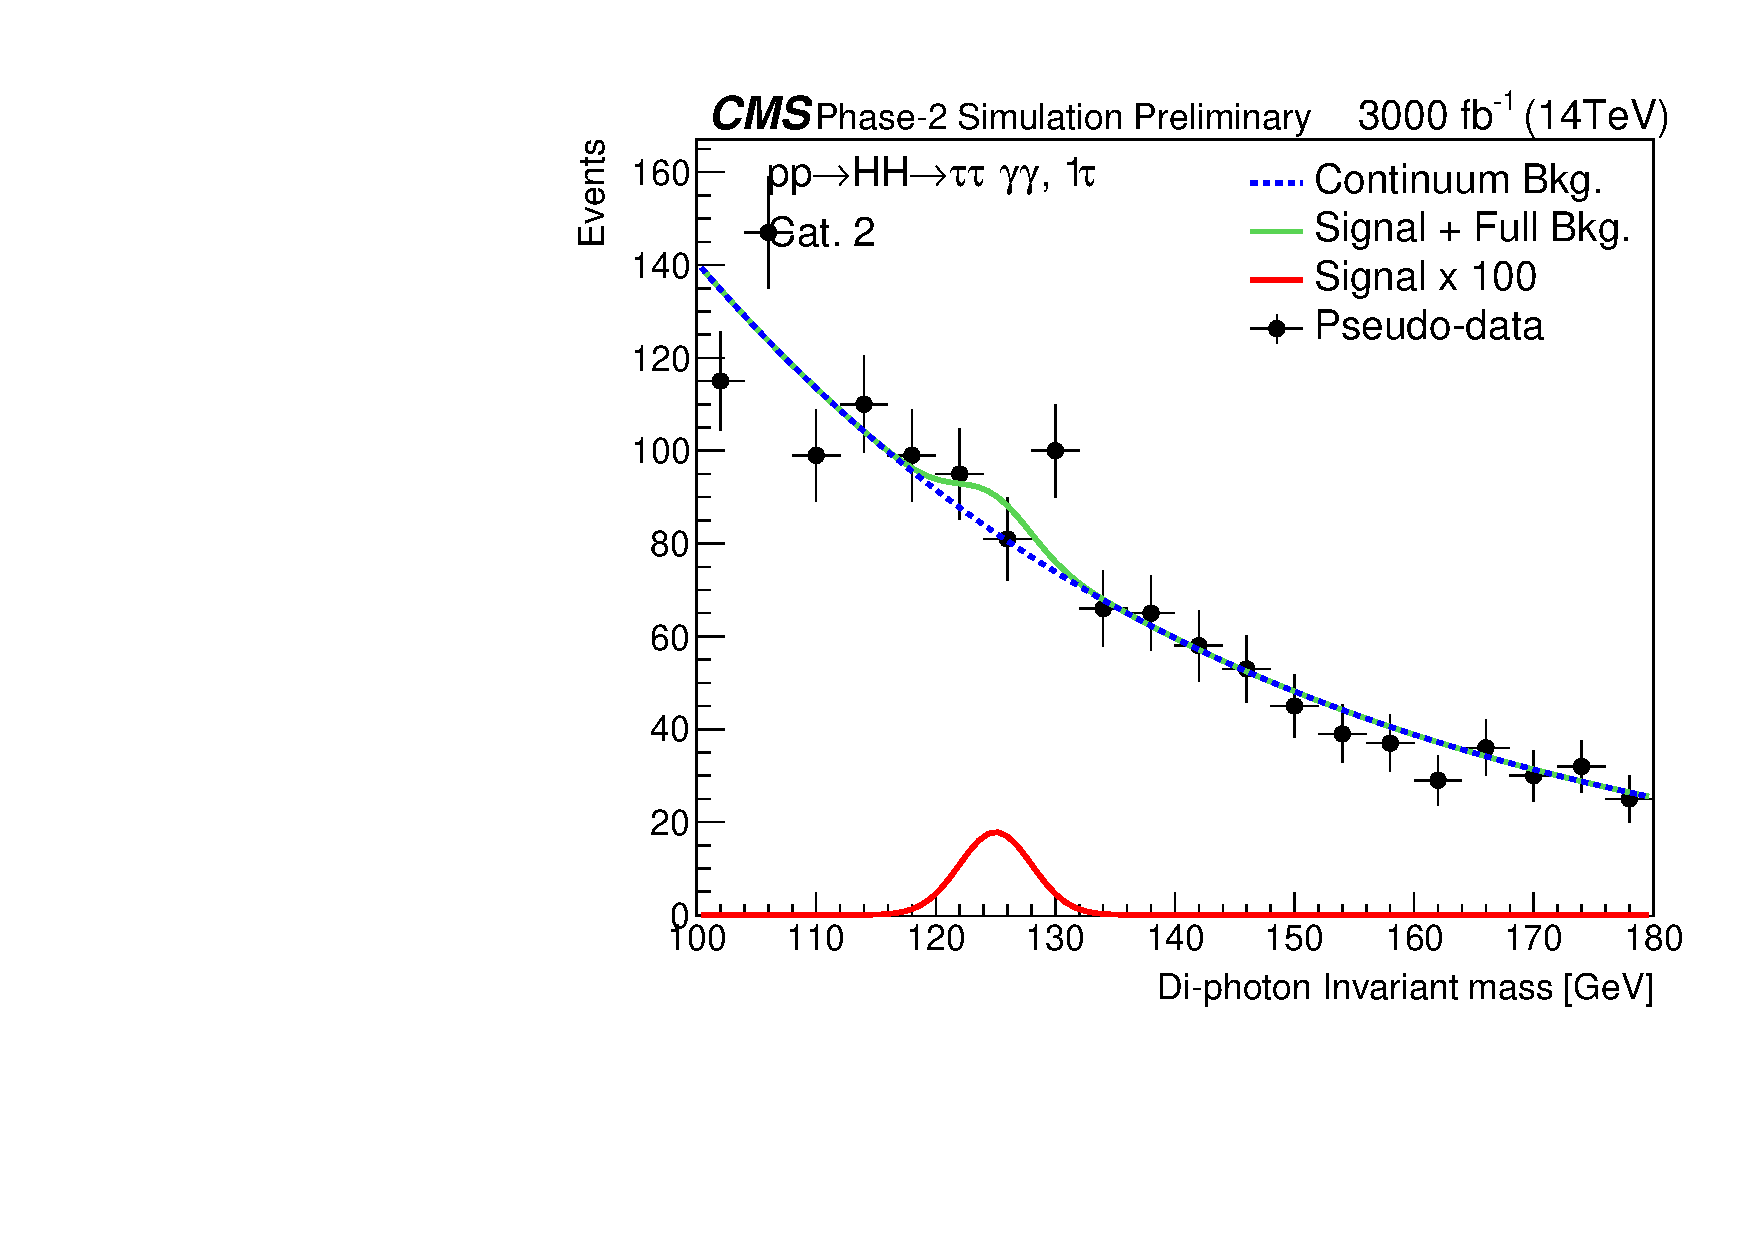
\includegraphics[width=\textwidth]{Mgg_c3_DNN_2_HL_FIT.pdf}
        \vspace{0.1cm}
        %\firstsubcaption{Preselection}
    \end{subfigure}
    \caption[]
    {\small \mgg fit distributions in the semi-leptonic final state's DNN category 4 (left) and in the single $\tau$ final state's DNN category 2 (right).}
    \label{fits}
\end{figure*}

\bibliographystyle{thesis_itubib}      % Designed .bst file 
\bibliography{thesis_bib}			   % .bib file

\eklerkapak{}
%\vglue18pt  % This has to be 18 pt - SBÖ
\singlespacing
\textbf{APPENDIX A.1 :} Python module of the analysis used in Bamboo framework and DNN setup for the \wwgg semi-leptonic final state \\
\textbf{APPENDIX A.2 :} Monte Carlo samples used in the analysis and cut-flow report in the semi-leptonic final state of $HH\rightarrow{WW\gamma\gamma}$ \\
\textbf{APPENDIX A.3 :} DNN input variables, their distributions, DNN performance plots and parameters for the semi-leptonic channel of $HH\rightarrow{WW\gamma\gamma}$\\
\textbf{APPENDIX A.4 :} Cut-flow report in the fully-leptonic final state of $HH\rightarrow{WW\gamma\gamma}$ \\
\textbf{APPENDIX A.5 :} DNN input variables, their distributions, DNN performance plots and the cut-flow table for the single $\tau$ channel of $HH\rightarrow{\tau\tau\gamma\gamma}$ \\
\textbf{APPENDIX A.6 :} Cut-flow report for the double $\tau$ channel of $HH\rightarrow{\tau\tau\gamma\gamma}$ \\
\textbf{APPENDIX A.7 :} Fit plots for each final state \\
\newpage

\eklerbolum{0}
\chapter{APPENDIX A.1}
\label{A1}
\vglue6pt

\begin{lstlisting}[language=Python, caption=Python module of the analysis used in Bamboo framework, label={bamboocode}]
import logging
from bamboo.analysisutils import loadPlotIt
import os.path
import copy
from bamboo.analysismodules import AnalysisModule, /
HistogramsModule


class SnowmassExample(CMSPhase2SimRTBHistoModule):
    def addArgs(self, parser):
        super().addArgs(parser)
        parser.add_argument("--mvaSkim",
                            action="store_true",
                            help="Produce skims")
        parser.add_argument("--datacards", action="store_true",
                            help="Produce histograms for datacards")
        parser.add_argument("--mvaEval", action="store_true",
                            help="Import MVA model and evaluate it")

    def definePlots(self, t, noSel, sample=None, sampleCfg=None):
        from bamboo.plots import Plot, CutFlowReport, SummedPlot
        from bamboo.plots import EquidistantBinning as EqB
        from bamboo import treefunctions as op

        plots = []

        noSel = noSel.refine("genweight",  weight=t.genweight)

        # yields
        yields_OneL = CutFlowReport(
            "yields_OneL", recursive=True, printInLog=True)
        yields_TwoL = CutFlowReport(
            "yields_TwoL", recursive=True, printInLog=True)
        yields_ZeroL = CutFlowReport(
            "yields_ZeroL", recursive=True, printInLog=True)
        yields_OneTau = CutFlowReport(
            "yields_OneTau", recursive=True, printInLog=True)
        yields_TwoTaus = CutFlowReport(
            "yields_TwoTaus", recursive=True, printInLog=True)

        yields_OneL.add(noSel, title='noSel')
        yields_TwoL.add(noSel, title='noSel')
        yields_ZeroL.add(noSel, title='noSel')
        yields_OneTau.add(noSel, title='noSel')
        yields_TwoTaus.add(noSel, title='noSel')

        plots.append(yields_OneL)
        plots.append(yields_TwoL)
        plots.append(yields_ZeroL)
        plots.append(yields_OneTau)
    plots.append(yields_TwoTaus)

    # select photons in the detector acceptance
    photons = op.select(t.gamma, lambda ph: op.AND(
        op.abs(ph.eta) < 2.5, ph.pt > 25.))

    # sort photons by pT
    sort_ph = op.sort(photons, lambda ph: -ph.pt)

    # select photons with loose ISO & ID
    isoPhotons = op.select(
        sort_ph, lambda ph: ph.isopass & (
        1 << 0))
    idPhotons = op.select(
        isoPhotons, lambda ph: ph.idpass & (1 << 0))

    # select electrons w loose ISO&ID and clean them
        # w.r.t good photons
    electrons = op.select(t.elec, lambda el: op.AND(
        el.pt > 10., op.abs(el.eta) < 2.5))
    sort_el = op.sort(electrons, lambda el: -el.pt)

    isoElectrons = op.select(
        clElectrons, lambda el: el.isopass & (1 << 0))

    idElectrons = op.select(
        isoElectrons, lambda el: el.idpass & (1 << 0))

    clElectrons = op.select(
        idElectrons, lambda el: op.AND(
        op.NOT(op.rng_any(
            idPhotons, lambda ph: op.deltaR(el.p4,ph.p4)<0.4)),
    ))

    # select muons with tight ISO & ID and clean them
        # w.r.t good photons and electrons
    muons = op.select(t.muon, lambda mu: op.AND(
        mu.pt > 10., op.abs(mu.eta) < 2.5))

    sort_mu = op.sort(clMuons, lambda mu: -mu.pt)

    isoMuons = op.select(idMuons, lambda mu: mu.isopass&(1<<2))

    idMuons = op.select(sort_mu, lambda mu: mu.idpass & (1 << 2))

    clMuons = op.select(muons, lambda mu: op.AND(
        op.NOT(op.rng_any(
            idPhotons, lambda ph: op.deltaR(mu.p4,ph.p4)<0.4)),
        op.NOT(op.rng_any(
            clElectrons,lambda j: op.deltaR(mu.p4,j.p4)<0.4))))

    # select taus with loose ISO and clean them
        #  w.r.t good photons & electrons & muons
    taus = op.sort(op.select(t.tau, lambda tau: op.AND(
        tau.pt > 20., op.abs(tau.eta)<2.5)),lambda tau:-tau.pt)

    isoTaus = op.select(clTaus,lambda tau: tau.isopass&(1<<2))

    clTaus = op.select(taus, lambda tau: op.AND(
        op.NOT(op.rng_any(
            idPhotons, lambda ph: op.deltaR(tau.p4, ph.p4) < 0.2)),
        op.NOT(op.rng_any(
            clElectrons, lambda el: op.deltaR(tau.p4, el.p4) < 0.2)),
        op.NOT(op.rng_any(
            clMuons, lambda mu: op.deltaR(tau.p4, mu.p4) < 0.2))
                                                ))

    # select jets with tight ID and clean 
        # them w.r.t good photons & electrons & muons & taus
    jets = op.select(t.jetpuppi, lambda jet: op.AND(
        jet.pt > 30., op.abs(jet.eta) < 5))

    sort_jets = op.sort(jets, lambda jet: -jet.pt)

    clJets = op.select(sort_jets, lambda j: op.AND(
        op.NOT(op.rng_any(
            idPhotons, lambda ph: op.deltaR(ph.p4, j.p4) < 0.4)),
        op.NOT(op.rng_any(
            clElectrons, lambda el: op.deltaR(el.p4, j.p4) < 0.4)),
        op.NOT(op.rng_any(
            clMuons, lambda mu: op.deltaR(mu.p4, j.p4) < 0.4)),
        op.NOT(op.rng_any(
            clTaus,
               lambda tau: op.deltaR(j.p4, tau.p4) < 0.4))
    ))

    idJets = op.select(clJets, lambda j: j.idpass & (1 << 2))

    # select b-jets with tight ID
    bJets = op.select(idJets, lambda j: j.btag & (1 << 1))

    # define variables for ease of use
    # di-photon invariant mass
    mGG = op.invariant_mass(idPhotons[0].p4, idPhotons[1].p4)
    mTauTau = op.invariant_mass(
        isoTaus[0].p4, isoTaus[1].p4)  # di-tau invariant mass
    pTGG = (op.sum(idPhotons[0].p4, idPhotons[1].p4)).pt()
    mJets = op.invariant_mass(
        idJets[0].p4, idJets[1].p4)  # di-jet invariant mass
    # sub-di-jet invariant mass
    mJets_SL = op.invariant_mass(idJets[1].p4, idJets[2].p4)

    # Fully leptonic FL invmasses
    # di-electron invariant mass
    mE = op.invariant_mass(idElectrons[0].p4, idElectrons[1].p4)
    # di-muon invariant mass
    mMu = op.invariant_mass(isoMuons[0].p4, isoMuons[1].p4)
    # e-mu system invariant mass
    mEMu = op.invariant_mass(idElectrons[0].p4, isoMuons[0].p4)

    # another set of variables
    nElec = op.rng_len(idElectrons)  # number of electrons
    nMuon = op.rng_len(isoMuons)  # number of muons
    nJet = op.rng_len(idJets)  # number of jets
    nTau = op.rng_len(isoTaus)  # number of taus

    pT_mGGL = op.product(idPhotons[0].pt, op.pow(mGG, -1))
    pT_mGGSL = op.product(idPhotons[1].pt, op.pow(mGG, -1))
    E_mGGL=op.product(idPhotons[0].p4.energy(),op.pow(mGG,-1))
    E_mGGSL=op.product(idPhotons[1].p4.energy(),op.pow(mGG,-1))

    # selections for efficiency check
    sel1_p = noSel.refine("2Photon", cut=op.AND(
        (op.rng_len(sort_ph) >= 2), (sort_ph[0].pt > 35.)))
    sel2_p = sel1_p.refine("idPhoton", cut=op.AND(
        (op.rng_len(idPhotons) >= 2), (idPhotons[0].pt > 35.)))

    # selections of the events with inv mass of photons 
        # in the 100-180 window
    hasInvM = sel2_p.refine("hasInvM", cut=op.AND(
        (op.in_range(100, op.invariant_mass(
            idPhotons[0].p4, idPhotons[1].p4), 180))
    ))

    ## Categories ##

    # selections for semileptonic final state
    semiLeptonic = hasInvM.refine("semiLeptonic",
    cut=op.OR(
        op.AND(nElec == 1, nMuon == 0),
        op.AND(nElec == 0, nMuon == 1)))
    yields_OneL.add(semiLeptonic, title='semiLeptonic')

    hasOneEl = hasInvM.refine(
        "hasOneEl", cut=op.AND(nElec == 1, nMuon == 0))
    hasOneMu = hasInvM.refine(
        "hasOneMu", cut=op.AND(nElec == 0, nMuon == 1))

    # selections for fully-leptonic final state
    fullyLeptonic = hasInvM.refine('fullyLeptonic',
    cut=op.AND(
        op.OR(
            op.AND(
                op.AND(nElec >= 2, nMuon == 0),
                idElectrons[0].charge != idElectrons[1].charge,
                op.NOT(
                op.deltaR(idElectrons[0].p4,idElectrons[1].p4)<0.4),
                op.OR(mE < 80, mE > 100), op.abs(m_eg - m_Z) > 5),
            op.AND(
                op.AND(nElec >= 1, nMuon == 1),
                idElectrons[0].charge != isoMuons[0].charge,
                op.NOT(op.deltaR(
                idElectrons[0].p4, isoMuons[0].p4) < 0.4),
                op.OR(mEMu<80,mEMu>100),op.abs(m_eg - m_Z)>5),
            op.AND(
                op.AND(nElec == 1, nMuon >= 1),
                idElectrons[0].charge != isoMuons[0].charge,
                op.NOT(op.deltaR(
                idElectrons[0].p4, isoMuons[0].p4) < 0.4),
                op.OR(mEMu<80,mEMu> 100), op.abs(m_eg - m_Z) > 5),
            op.AND(
                op.AND(nMuon >= 2, nElec == 0),
                isoMuons[0].charge != isoMuons[1].charge,
                op.NOT(op.deltaR(isoMuons[0].p4,isoMuons[1].p4)<0.4),
                op.OR(mMu<80,mMu>100))),
        pTGG > 91,
        op.AND(thirdEl < 10, thirdMu < 10),
        op.rng_len(bJets) < 1,
        met[0].pt > 20
    ))

    ##### fully-leptonic final state variables #####
    m_eg = op.invariant_mass(idElectrons[0].p4, idPhotons[0].p4)
    m_Z = 91.18

    thirdEl = op.switch(op.rng_len(idElectrons) < 3,
                        op.c_float(0.), idElectrons[2].pt)
    thirdMu = op.switch(op.rng_len(isoMuons) < 3,
                        op.c_float(0.), isoMuons[2].pt)
    #############################################

    yields_TwoL.add(fullyLeptonic, title='fullyLeptonic')

    # selections for tautau final states
    c3 = hasInvM.refine("hasOneTauNoLept", cut=op.AND(
        nTau == 1,
        op.rng_len(idElectrons) == 0,
        op.rng_len(isoMuons) == 0))
    yields_OneTau.add(c3, "One Tau No Lept")

    c4 = hasInvM.refine("hasTwoTaus", cut=op.AND(
        nTau >= 2,
        op.rng_len(idElectrons) == 0,
        op.rng_len(isoMuons) == 0))
    yields_TwoTaus.add(c4, "Two Taus")

    ########## Z veto ##########
    c4_Zveto = c4.refine("hasTwoTaus_Zveto", cut=op.NOT(
        op.in_range(80, mTauTau, 100)))

    ## End of Categories ##

    # plots
    # semiLeptonic
    plots.append(Plot.make1D(
        "LeadingPhotonPtOneL",
        idPhotons[0].pt,
        semiLeptonic,
        EqB(30, 0., 300.),
        title="Leading Photon pT")
        )
    plots.append(
        Plot.make1D(
            "SubLeadingPhotonPtOneL",
            idPhotons[1].pt, semiLeptonic, EqB(
        30, 0., 300.), title="SubLeading Photon pT"))
    plots.append(
        Plot.make1D(
            "LeadingPhotonEtaOneL",
            idPhotons[0].eta, semiLeptonic, EqB(
        80, -4., 4.), title="Leading Photon eta"))
    plots.append(
        Plot.make1D(
            "SubLeadingPhotonEtaOneL",
            idPhotons[1].eta, semiLeptonic, EqB(
        80, -4., 4.), title="SubLeading Photon eta"))
    plots.append(
        Plot.make1D(
            "LeadingPhotonPhiOneL",
            idPhotons[0].phi, semiLeptonic, EqB(
        100, -3.5, 3.5), title="Leading Photon phi"))
    plots.append(
        Plot.make1D(
            "SubLeadingPhotonPhiOneL",
            idPhotons[1].phi, semiLeptonic, EqB(
        100, -3.5, 3.5), title="SubLeading Photon phi"))
    plots.append(
        Plot.make1D(
            "nElectronsOneL",
            nElec,
            semiLeptonic,
            EqB(10, 0., 10.), title="Number of electrons"))
    plots.append(
        Plot.make1D(
            "nMuonsOneL",
            nMuon, semiLeptonic,
                 EqB(10, 0., 10.), title="Number of Muons"))
    plots.append(
        Plot.make1D(
            "nJetsOneL",
            nJet, semiLeptonic,
                 EqB(10, 0., 10.), title="Number of Jets"))
    plots.append(
        Plot.make1D(
            "LeadingPhotonpT_mGGLsemiLeptonic",
            pT_mGGL, semiLeptonic, EqB(100, 0., 5.),
            title="Leading Photon p_{T}/m_{\gamma\gamma}"))
    plots.append(
        Plot.make1D(
            "SubLeadingPhotonpT_mGGLsemiLeptonic",
            pT_mGGSL, semiLeptonic, EqB(100, 0., 5.),
            title="SubLeading Photon p_{T}/m_{\gamma\gamma}"))
    plots.append(
        Plot.make1D(
            "LeadingPhotonE_mGGLsemiLeptonic",
            E_mGGL, semiLeptonic, EqB(100, 0., 5.),
        title="Leading Photon E/m_{\gamma\gamma}"))
    plots.append(
        Plot.make1D(
            "SubLeadingPhotonE_mGGLsemiLeptonic",
            E_mGGSL, semiLeptonic, EqB(100, 0., 5.),
            title="SubLeading Photon E/m_{\gamma\gamma}"))
    plots.append(
        Plot.make1D(
            "MET",
            metPt, semiLeptonic,
            EqB(80, 0., 800.), title="MET"))
    plots.append(
        Plot.make1D(
            "Inv_mass_ggsemiLeptonic",
            mGG, semiLeptonic,
            EqB(80, 100., 180.), title="m_{\gamma\gamma}"))
    plots.append(
        Plot.make1D(
            "Inv_mass_ggsemiLeptonic_135",
            mGG,
            semiLeptonic, EqB(20, 115., 135.),
            title="m_{\gamma\gamma}"))

    # Leading electron Plots
    plots.append(Plot.make1D(
        "ElectronpT", idElectrons[0].pt, hasOneEl,
        EqB(30, 0., 300.), title='Leading Electron pT'))
    plots.append(Plot.make1D(
        "ElectronE", idElectrons[0].p4.E(),hasOneEl,
        EqB(50, 0., 500.), title='Leading Electron E'))
    plots.append(Plot.make1D(
        "ElectronEta", idElectrons[0].eta, hasOneEl,
        EqB(80, -4., 4.), title='Leading Electron eta'))
    plots.append(Plot.make1D(
        "ElectronPhi", idElectrons[0].phi, hasOneEl,
        EqB(100, -3.5, 3.5), title='Leading Electron phi'))

    # Leading muon Plots
    plots.append(Plot.make1D(
        "MuonpT", isoMuons[0].pt, hasOneMu, EqB(
        30, 0., 100.), title='Leading Muon pT'))
    plots.append(Plot.make1D(
        "MuonE", isoMuons[0].p4.E(), hasOneMu, EqB(
        50, 0., 500.), title='Leading Muon E'))
    plots.append(Plot.make1D(
        "MuonEta", isoMuons[0].eta, hasOneMu, EqB(
        80, -4., 4.), title='Leading Muon eta'))
    plots.append(Plot.make1D(
        "MuonPhi", isoMuons[0].phi, hasOneMu, EqB(
        100, -3.5, 3.5), title='Leading Muon phi'))

    ### DNN variables ###

    semiLeptonic = hasInvM.refine("semiLeptonic", cut=op.OR(
        op.AND(nElec == 1, nMuon == 0),
        op.AND(nElec == 0, nMuon == 1)
        
        ))

   hasOneJ = semiLeptonic.refine(
        "semiLeptonic_hasOneJ", cut=op.rng_len(idJets) == 1)
    hasTwoJ = semiLeptonic.refine(
        "semiLeptonic_hasTwoJ", cut=op.rng_len(idJets) == 2)
    hasthreeJ = semiLeptonic.refine(
        "semiLeptonic_hasthreeJ", cut=op.rng_len(idJets) == 3)

    plots.append(Plot.make1D(
        "semiLeptonic_hasOneJ_jetpt",
        idJets[0].pt, hasOneJ, EqB(
        30, 0., 300.), title="Leading Jet p_T"))
    plots.append(Plot.make1D(
        "semiLeptonic_hasOneJ_jeteta",
        idJets[0].eta, hasOneJ, EqB(
        80, -5.5, 5.5), title="Leading Jet #eta"))
    plots.append(Plot.make1D(
        "semiLeptonic_hasOneJ_jetphi",
        idJets[0].phi, hasOneJ, EqB(
        100, -3.5, 3.5), title="Leading Jet #phi"))
    plots.append(Plot.make1D(
        "semiLeptonic_hasOneJ_jetE",
        idJets[0].p4.E(
    ), hasOneJ, EqB(50, 0., 500.), title="Leading Jet Energy"))

    plots.append(Plot.make1D(
        "semiLeptonic_hasTwoJ_jetpt",
        idJets[1].pt, hasTwoJ, EqB(
        30, 0., 300.), title="Sub-leading Jet p_T"))
    plots.append(Plot.make1D(
        "semiLeptonic_hasTwoJ_jeteta",
        idJets[1].eta, hasTwoJ, EqB(
        80, -5.5, 5.5), title="Sub-leading Jet #eta"))
    plots.append(Plot.make1D(
        "semiLeptonic_hasTwoJ_jetphi",
        idJets[1].phi, hasTwoJ, EqB(
        100, -3.5, 3.5), title="Sub-leading Jet #phi"))
    plots.append(Plot.make1D(
        "semiLeptonic_hasTwoJ_jetE",
        idJets[1].p4.E(
    ), hasTwoJ, EqB(50, 0., 500.), title="Sub-leading Jet Energy"))

    plots.append(Plot.make1D(
        "semiLeptonic_hastwoJ_mjj", op.invariant_mass(
        idJets[0].p4, idJets[1].p4), hasTwoJ,
        EqB(100, 0., 1000.), title="Di-jet invariant mass"))
    plots.append(Plot.make1D(
        "semiLeptonic_hasthreeJ_mjj", op.invariant_mass(
        idJets[1].p4, idJets[2].p4), hasthreeJ,
        EqB(100, 0., 1000.), title="Tri-jet invariant mass"))

    c3 = hasInvM.refine("hasOneTauNoLept", cut=op.AND(
        nTau == 1, op.rng_len(idElectrons) == 0,
        op.rng_len(isoMuons) == 0)
        )
    c3_OneJ = c3.refine("c3hasOneJ", cut=op.rng_len(idJets) == 1)
    c3_TwoJ = c3.refine("c3hasTwoJ", cut=op.rng_len(idJets) == 2)

    plots.append(Plot.make1D("c3_nJet", nJet, c3, EqB(
        10, 0., 10.), title="Number of Jets"))
    plots.append(Plot.make1D("c3_nbJet", op.rng_len(bJets), c3,
                 EqB(10, 0., 10.), title="Number of b-tagged Jets"))
    plots.append(Plot.make1D(
        "c3_met", met[0].pt, c3, EqB(
        80, 0., 800.), title="Missing Transverse Energy"))
    plots.append(Plot.make1D(
        "c3_pt_mgg", pT_mGGL, c3, EqB(
        100, 0., 5.),
        title="Leading Photon p_{T}/m_{\gamma\gamma}"))
    plots.append(Plot.make1D(
        "c3_SLpt_mgg", pT_mGGSL, c3, EqB(
        100, 0., 5.),
        title="Sub-leading Photon p_{T}/m_{\gamma\gamma}"))
    plots.append(Plot.make1D(
        "c3_leadingphoton_eta", idPhotons[0].eta, c3, EqB(
        80, -4., 4.), title="Leading Photon \eta"))
    plots.append(Plot.make1D(
        "c3_subleadingphoton_eta", idPhotons[1].eta, c3, EqB(
        80, -4., 4.), title="Sub-leading Photon \eta"))
    plots.append(Plot.make1D(
        "c3_leadingphoton_phi", idPhotons[0].phi, c3, EqB(
        100, -3.5, 3.5), title="Leading Photon \phi"))
    plots.append(Plot.make1D(
        "c3_subleadingphoton_phi", idPhotons[1].phi, c3, EqB(
        100, -3.5, 3.5), title="Sub-leading Photon \phi"))
    plots.append(Plot.make1D(
        "c3_LE_mgg", E_mGGL, c3, EqB(
        100, 0., 5.),
        title="Leading Photon E/m_{\gamma\gamma}"))
    plots.append(Plot.make1D(
        "c3_SLE_mgg", E_mGGSL, c3, EqB(
        100, 0., 5.),
        title="Sub-leading Photon E/m_{\gamma\gamma}"))
    plots.append(Plot.make1D(
        "c3_leadingtau_E", isoTaus[0].p4.E(), c3, EqB(
        50, 0., 500.), title="Leading Tau Energy"))
    plots.append(Plot.make1D(
        "c3_leadingtau_eta", isoTaus[0].eta, c3, EqB(
        80, -4., 4.), title="Leading Tau \eta"))
    plots.append(Plot.make1D(
        "c3_leadingtau_phi", isoTaus[0].phi, c3, EqB(
        100, -3.5, 3.5), title="Leading Tau \phi"))
    plots.append(Plot.make1D(
        "c3_leadingtau_pt", isoTaus[0].pt, c3, EqB(
        50, 0., 500.), title="Leading Tau p_T"))
    plots.append(Plot.make1D(
        "c3_oneJet_Ljetpt", idJets[0].pt, c3_OneJ, EqB(
        50, 0., 500.), title="Leading Jet p_T"))
    plots.append(Plot.make1D(
        "c3_oneJet_Ljeteta", idJets[0].eta, c3_OneJ, EqB(
        80, -5.5, 5.5), title="Leading Jet \eta"))
    plots.append(Plot.make1D(
        "c3_twoJet_SLjetpt", idJets[1].pt, c3_TwoJ, EqB(
        50, 0., 500.), title="Sub-leading Jet p_T"))
    plots.append(Plot.make1D(
        "c3_twoJet_SLjeteta", idJets[1].eta, c3_TwoJ, EqB(
        80, -5.5, 5.5), title="Sub-leading Jet \eta"))

    plots.append(Plot.make1D(
        "fullyLeptonic_mgg", mGG, fullyLeptonic, EqB(
        80, 100., 180.),
        title="Di-photon invariant mass [GeV]"))
    plots.append(Plot.make1D(
        "Inv_mass_ggfullyLeptonic", mGG, fullyLeptonic,
                 EqB(80, 100., 180.),
                 title="m_{\gamma\gamma}"))
    plots.append(Plot.make1D(
        "mGG_c3", mGG, c3, EqB(80, 100, 180),
                 title="M_{\gamma\gamma}",
                 plotopts={"log-y": True}))
    plots.append(Plot.make1D(
        "mGG_c4", mGG, c4, EqB(80, 100, 180),
                 title="M_{\gamma\gamma}",
                 plotopts={"log-y": True}))

    mvaVars_semiLeptonic = {
        "weight": noSel.weight,
        "Eta_ph1": idPhotons[0].eta,
        "Phi_ph1": idPhotons[0].phi,
        "E_mGG_ph1": E_mGGL,
        "pT_mGG_ph1": pT_mGGL,
        "Eta_ph2": idPhotons[1].eta,
        "Phi_ph2": idPhotons[1].phi,
        "E_mGG_ph2": E_mGGSL,
        "pT_mGG_ph2": pT_mGGSL,
        "Electron_E": op.switch(
            op.rng_len(idElectrons) == 0,
            op.c_float(0.), idElectrons[0].p4.E()),
        "Electron_pT": op.switch(
            op.rng_len(idElectrons) == 0,
            op.c_float(0.), idElectrons[0].pt),
        "Electron_Eta": op.switch(
            op.rng_len(idElectrons) == 0,
            op.c_float(0.), idElectrons[0].eta),
        "Electron_Phi": op.switch(
            op.rng_len(idElectrons) == 0,
            op.c_float(0.), idElectrons[0].phi),
        "Muon_E": op.switch(
            op.rng_len(isoMuons) == 0,
            op.c_float(0.), isoMuons[0].p4.E()),
        "Muon_pT": op.switch(
            op.rng_len(isoMuons) == 0,
            op.c_float(0.), isoMuons[0].pt),
        "Muon_Eta": op.switch(
            op.rng_len(isoMuons) == 0,
            op.c_float(0.), isoMuons[0].eta),
        "Muon_Phi": op.switch(
            op.rng_len(isoMuons) == 0,
            op.c_float(0.), isoMuons[0].phi),
        "nJets": nJet,
        "E_jet1": op.switch(
            op.rng_len(idJets) == 0,
            op.c_float(0.), idJets[0].p4.E()),
        "pT_jet1": op.switch(
            op.rng_len(idJets) == 0,
            op.c_float(0.), idJets[0].pt),
        "Eta_jet1": op.switch(
            op.rng_len(idJets) == 0,
            op.c_float(0.), idJets[0].eta),
        "Phi_jet1": op.switch(
            op.rng_len(idJets) == 0,
            op.c_float(0.), idJets[0].phi),
        "E_jet2": op.switch(
            op.rng_len(idJets) < 2,
            op.c_float(0.), idJets[1].p4.E()),
        "pT_jet2": op.switch(
            op.rng_len(idJets) < 2,
            op.c_float(0.), idJets[1].pt),
        "Eta_jet2": op.switch(
            op.rng_len(idJets) < 2,
            op.c_float(0.), idJets[1].eta),
        "Phi_jet2": op.switch(
            op.rng_len(idJets) < 2,
            op.c_float(0.), idJets[1].phi),
        "InvM_jet": op.switch(
            op.rng_len(idJets) < 2,
            op.c_float(0.), mJets),
        "InvM_jet2": op.switch(
            op.rng_len(idJets) < 3,
            op.c_float(0.), mJets_SL),
        "met": metPt
    }

    mvaVars_singleTau = {
        "weight": noSel.weight,
        # Event level variables
        "nJets": nJet,
        "nBJets": op.rng_len(bJets),
        "metPt": metPt,
        # Photon and di-Photon variables
        "L_pt_mGG": pT_mGGL,
        "L_photon_eta": idPhotons[0].eta,
        "L_photon_phi": idPhotons[0].phi,
        "E_mGG_ph1": E_mGGL,
        "E_mGG_ph2": E_mGGSL,
        "SL_pt_mGG": pT_mGGSL,
        "SL_photon_eta": idPhotons[1].eta,
        "SL_photon_phi": idPhotons[1].phi,
        "LTauE": isoTaus[0].p4.E(),
        "LtauPt": isoTaus[0].pt,
        "LtauEta": isoTaus[0].eta,
        "LtauPhi": isoTaus[0].phi,
        "Ljet_Pt": op.switch(
            nJet == 0, op.c_float(0.), idJets[0].pt),
        "Ljet_Eta": op.switch(
            nJet == 0, op.c_float(0.), idJets[0].eta),
        "SLjet_Pt": op.switch(
            nJet < 2, op.c_float(0.), idJets[1].pt),
        "SLjet_Eta": op.switch(
            nJet < 2, op.c_float(0.), idJets[1].eta),
    }

    # save mvaVars to be retrieved later in the
    # postprocessor and save in a parquet file
    if self.args.mvaSkim:
        from bamboo.plots import Skim
        plots.append(Skim("Skim", mvaVars_semiLeptonic, 
        semiLeptonic))
        plots.append(Skim("c3", mvaVars_singleTau, c3))

    # evaluate dnn model on data
    if self.args.mvaEval:
        #from IPython import embed
        WW_DNNmodel_path_even = 
            "~/DNN_WW/even_model_test3.onnx"
        WW_DNNmodel_path_odd = 
            "~/DNN_WW/odd_model_test3.onnx"
        tt_DNNmodel_path_even = 
            "~/DNN_Tau/even_model_test3.onnx"
        tt_DNNmodel_path_odd = 
            "~/DNN_Tau/odd_model_test3.onnx"

        mvaVars_semiLeptonic.pop("weight", None)
        mvaVars_singleTau.pop("weight", None)
        mvaVars_semiLeptonic_FH.pop("weight", None)
        from bamboo.root import loadHeader
        loadHeader(
            "~/WWGG/header_split.h")

        split_evaluator = op.extMethod('split::Ph1_phi')
        split = split_evaluator(idPhotons[0].phi)

        if split == 0:
            tt_model = tt_DNNmodel_path_even
            WW_model = WW_DNNmodel_path_even
        else:
            tt_model = tt_DNNmodel_path_odd
            WW_model = WW_DNNmodel_path_odd

        dnn_ww = op.mvaEvaluator(
            WW_model, mvaType="ONNXRuntime",
            otherArgs="predictions")
        inputs_ww = op.array(
            'float',
            *[op.static_cast('float', val)
             for val in mvaVars_semiLeptonic.values()])
        output_ww = dnn_ww(inputs_ww)

        dnn_tt = op.mvaEvaluator(
            tt_model, mvaType="ONNXRuntime", otherArgs="predictions")
        inputs_tt = op.array(
            'float',
            *[op.static_cast('float', val)
             for val in mvaVars_singleTau.values()])
        output_tt = dnn_tt(inputs_tt)

        ########  semiLeptonic_DNN ########

        hasDNNscore1 = semiLeptonic.refine(
            "hasDNNscore1", cut=op.in_range(0.1, output_ww[0], 0.6))
        yields_OneL.add(hasDNNscore1, title='hasDNNscore1')

        hasDNNscore2 = semiLeptonic.refine(
            "hasDNNscore2", cut=op.in_range(0.6, output_ww[0], 0.8))
        yields_OneL.add(hasDNNscore2, title='hasDNNscore2')

        hasDNNscore3 = semiLeptonic.refine(
            "hasDNNscore3", cut=op.in_range(0.8, output_ww[0], 0.92))
        yields_OneL.add(hasDNNscore3, title='hasDNNscore3')

        hasDNNscore4 = semiLeptonic.refine(
            "hasDNNscore4", cut=output_ww[0] > 0.92)
        yields_OneL.add(hasDNNscore4, title='hasDNNscore4')

        ######## OneTau_DNN ########

        hasDNNscore1_tt = c3.refine(
            "hasDNNscore_tt", cut=op.in_range(0.1, output_tt[0], 
            0.65))
        yields_OneTau.add(hasDNNscore1_tt, title='hasDNNscore_tt')

        hasDNNscore2_tt = c3.refine(
            "hasDNNscore2_tt", cut=output_tt[0] > 0.65)
        yields_OneTau.add(hasDNNscore2_tt, title='hasDNNscore2_tt')

        plots.append(Plot.make1D("dnn_score_ww",
                     output_ww[0], semiLeptonic, EqB(40, 0, 1.)))
        plots.append(Plot.make1D("dnn_score_tt",
                     output_tt[0], c3, EqB(40, 0, 1.)))

        plots.append(Plot.make1D("Inv_mass_semiLeptonic_DNN_1",
        mGG, hasDNNscore1, EqB(
            80, 100., 180.), title="m_{\gamma\gamma}"))
        plots.append(Plot.make1D("Inv_mass_semiLeptonic_DNN_2",
        mGG, hasDNNscore2, EqB(
            80, 100., 180.), title="m_{\gamma\gamma}"))
        plots.append(Plot.make1D("Inv_mass_semiLeptonic_DNN_3",
        mGG, hasDNNscore3, EqB(
            80, 100., 180.), title="m_{\gamma\gamma}"))
        plots.append(Plot.make1D("Inv_mass_semiLeptonic_DNN_4",
        mGG, hasDNNscore4, EqB(
            80, 100., 180.), title="m_{\gamma\gamma}"))

        plots.append(Plot.make1D("Inv_mass_singleTau_c3_DNN_1",
        mGG, hasDNNscore1_tt, EqB(
            80, 100., 180.), title="m_{\gamma\gamma}"))
        plots.append(Plot.make1D("Inv_mass_singleTau_c3_DNN_2",
        mGG, hasDNNscore2_tt, EqB(
            80, 100., 180.), title="m_{\gamma\gamma}"))

        from bamboo.plots import Skim

    return plots

\end{lstlisting}

\begin{lstlisting}[language=Python, caption=DNN setup for the \wwgg semi-leptonic final state, label={dnncode}]
import os
import yaml
import importlib
import matplotlib.pyplot as plt
from matplotlib.backends.backend_pdf import PdfPages
import numpy as np
import pyarrow.parquet as pq
import pandas as pd
from sklearn.model_selection import train_test_split
from sklearn.preprocessing import LabelEncoder, OneHotEncoder 
import tensorflow as tf
from tensorflow import keras
from tensorflow.keras import layers
from tensorflow.keras.callbacks import EarlyStopping,
    ReduceLROnPlateau

### Parameters of the training ###
#split = "even" 
split = "odd" 

suffix = 'test3'

quantile = 1.0

tags = ['HH','background','single H']
importance = [1.,1.,1.] # Importance of each category

# DNN hyperparameters #
parameters = {
    'epochs'                : 200,
    'lr'                    : 0.001,
    'batch_size'            : 256,
    'n_layers'              : 3,
    'n_neurons'             : 64,
    'hidden_activation'     : 'relu',
    'output_activation'     : 'softmax',
    'l2'                    : 1e-6,
    'dropout'               : 0.,
    'batch_norm'            : True,
}

# Input variables
input_vars=["Eta_ph1",
            "Phi_ph1",
            "E_mGG_ph1",
            "pT_mGG_ph1",
            "Eta_ph2",
            "Phi_ph2",
            "E_mGG_ph2",
            "pT_mGG_ph2",
            "Electron_E",
            "Electron_pT",
            "Electron_Eta",
            "Electron_Phi",
            "Muon_E",
            "Muon_pT",
            "Muon_Eta",
            "Muon_Phi",
            "nJets",
            "E_jet1",
            "pT_jet1",
            "Eta_jet1",
            "Phi_jet1",
            "E_jet2",
            "pT_jet2",
            "Eta_jet2",
            "Phi_jet2",
            "InvM_jet",
            "InvM_jet2",
            "met"]
# Load the required data #
outputPath = '~/bamboodev/WWGG/Clean_Skim'
skimFile = os.path.join(outputPath,'results','Skim.parquet')
yamlFile = os.path.join(outputPath,'plots.yml')

# Load dataframe from parquet #
df = pd.read_parquet(skimFile)

# Load samples + plots data from yaml file #
with open(yamlFile,'r') as handle:
    config = yaml.full_load(handle)

# Cut negative event weights #
df = df[df['weight']>0]

# Add tag column #
if 'tag' in df.columns:
    del df['tag']

df['tag'] = 'background'
for singleH in ['VBFH','VH','THQ','GluGluHTo','ttHJet']:
    df.loc[df.process.str.contains(singleH),['tag']] = 'single H'
df.loc[df.process.str.contains('HH'),['tag']] = 'HH'

for tag in tags:
    if tag in df.columns:
        del df[tag]

assert len(set(tags).intersection(set(pd.unique(df['tag'])))) == \
    len(tags)
label_encoder  = LabelEncoder()
onehot_encoder = OneHotEncoder(sparse=False)
label_encoder.fit(tags)
integers = label_encoder.transform(df['tag']).reshape(-1, 1)
onehot_encoder.fit(np.arange(len(tags)).reshape(-1, 1))
onehot = onehot_encoder.transform(integers)
onehot_df = pd.DataFrame(onehot,columns=tags,index=df.index)

df = pd.concat((df,onehot_df),axis=1)

df['event_weight'] = df['weight'].copy()

if (df['event_weight'] < 0).sum() > 0:
    raise RuntimeError(f"There are {(df['event_weight']<0).sum()}\
        events with negative event weight, this should not happen")

# Compute training weight #
if 'training_weight' in df.columns:
    del df['training_weight']
df['training_weight'] = df['event_weight'].copy()

for itag,tag in enumerate(tags):
    df.loc[df['tag']==tag,'training_weight'] *= importance[itag] \
        * df.shape[0]/ len(tags) / df[df['tag']==tag]/
        ['event_weight'].sum()

df = df[(df['weight']>0) & (df['training_weight']<200)]

import utils
importlib.reload(utils)
print ('Using event weight')
utils.checkBatches(df,label_column='tag',weight_column=/
'event_weight',batch_size=parameters['batch_size'])
print ('Using training weight')
utils.checkBatches(df,label_column='tag',/
weight_column='training_weight',\
    batch_size=parameters['batch_size'])

# Plot the background and signal weights #
fig,axs = plt.subplots(figsize=(16,8),nrows=len(tags),ncols=3)
fig.subplots_adjust(left=0.1, right=0.9, top=0.98, bottom=0.1,/
wspace=0.2, hspace=0.4)
for irow,tag in enumerate(tags):
    for icol,column in enumerate(['weight','event_weight',/
    'training_weight']):
        axs[irow,icol].hist(df[df['tag']==tag][column],/
        bins=100,color='b')
        axs[irow,icol].set_title(f"Category = {tag}")
        axs[irow,icol].set_xlabel(column)
        axs[irow,icol].set_yscale('log')
fig.savefig("event_weights_A.pdf", dpi = 300)

# Determine splitting variable #
split_var = df['Phi_ph1'].copy()
split_var = np.abs(split_var)
split_var *= 1e4
split_var -= np.floor(split_var) 
split_var = (split_var*1e1).astype(int)
split_var = split_var %2 == 0
print (f'Even set has {df[split_var].shape[0]:10d} events \
    [{df[split_var].shape[0]/df.shape[0]*100:5.2f}%]')
print (f'Odd  set has {df[~split_var].shape[0]:10d} events \
    [{df[~split_var].shape[0]/df.shape[0]*100:5.2f}%]')

# Sets splitting #
print (f'Using split type {split}')
if split == 'even':
    train_df = df[~split_var] # Trained on odd
    test_df  = df[split_var]  # Evaluated on even 
elif split == 'odd':
    train_df = df[split_var]  # Trained on even
    test_df  = df[~split_var] # Evaluated on odd 
else:
    raise RuntimeError(f'Split needs to be either odd or even')

# Randomise for training
train_df = train_df.sample(frac=1)

# Quantile corrections
quantile_lim = train_df['training_weight'].quantile(quantile)
print (f'{(1-quantile)*100:5.2f}% right quantile is when/
weight is at {quantile_lim}')
print ('  -> These events will be repeated and their/
learning weights reduced accordingly to avoid unstability') 

# Select the events #
idx_to_repeat = train_df['training_weight'] >= quantile_lim                          
events_excess = train_df[idx_to_repeat].copy()

saved_columns = train_df[['training_weight','process']].copy()

# Compute multiplicative factor #
factor = (events_excess['training_weight']/quantile_lim)/
.values.astype(np.int32) 

# Correct the weights of events already in df #
train_df.loc[idx_to_repeat,'training_weight'] /= factor

# Add N-1 copies #
arr_to_repeat = train_df[idx_to_repeat].values                                       
repetition = np.repeat(np.arange(arr_to_repeat.shape[0]), factor-1)                   
df_repeated = pd.DataFrame(np.take(arr_to_repeat,repetition,axis=0),
columns=train_df.columns)
df_repeated = df_repeated.astype(train_df.dtypes.to_dict())
train_df = pd.concat((train_df,df_repeated),axis=0,/
ignore_index=True).sample(frac=1).reset_index()

# Printout #
print ('Changes per process in training set')
for process in pd.unique(train_df['process']):
    N_before = saved_columns[saved_columns['process']==process]/
    .shape[0]
    N_after  = train_df[train_df['process']==process].shape[0]
    if N_before != N_after:
        print (f"{process:20s}")
        print (f"... {N_before:6d} events [sum weight = \
            {saved_columns[saved_columns['process']==process]\
                ['training_weight'].sum():14.6f}]",end=' -> ')
        print (f"{N_after:6d} events [sum weight = \
            {train_df[train_df['process']==process]\
                ['training_weight'].sum():14.6f}]")
    
print ()
print (f"Total entries : {saved_columns.shape[0]:14d} -> \
    {train_df.shape[0]:14d}")
print (f"Total event sum : {saved_columns['training_weight']\
    .sum():14.6f} -> {train_df['training_weight'].sum():14.6f}")

# Validation split #
train_df,val_df  = train_test_split(train_df,test_size=0.3)

# Printout #
print ('\nFinal sets')
print (f'Training set   = {train_df.shape[0]}')
print (f'Validation set = {val_df.shape[0]}')
print (f'Testing set    = {test_df.shape[0]}')
print (f'Total set      = {df.shape[0]}')

# Plot the background and signal weights #
fig,axs = plt.subplots(figsize=(16,8),nrows=1,ncols=2)
fig.subplots_adjust(left=0.1, right=0.9, top=0.96, bottom=0.1,
                    wspace=0.2,hspace=0.3)

if split == 'even':
    axs[0].hist(df[~split_var]['training_weight'],bins=100,color='b')
elif split == 'odd':
    axs[0].hist(df[split_var]['training_weight'],bins=100,color='b')
axs[0].set_title("Before correction")
axs[0].set_xlabel("Training weight")
axs[0].set_yscale('log')
axs[1].hist(train_df['training_weight'],bins=100,color='b')
axs[1].set_title("After correction")
axs[1].set_xlabel("Training weight")
axs[1].set_yscale('log')
fig.savefig("event_weights_C.pdf", dpi = 300)

# Input layer #
inputs = keras.Input(shape=(len(input_vars),), name="particles")

# Preprocessing layer
from tensorflow.keras.layers.experimental import preprocessing
normalizer = preprocessing.Normalization\
    (mean     = train_df[input_vars].mean(axis=0),
    variance = train_df[input_vars].var(axis=0),
    name     = 'Normalization')(inputs)
    # this layer does the preprocessing (x-mu)/std for each input
# Dense (hidden) layers #
x = normalizer
for i in range(parameters['n_layers']):
    x = layers.Dense(
        units                = parameters['n_neurons'], 
        activation           = parameters['hidden_activation'], 
        activity_regularizer = tf.keras.regularizers/
        .l2(parameters['l2']),
        name                 = f"dense_{i}")(x)
    if parameters['batch_norm']:
        x = layers.BatchNormalization()(x)
    if parameters['dropout'] > 0.:
        x = layers.Dropout(parameters['dropout'])(x)
# Output layer #
outputs = layers.Dense(
    units                = 3, 
    activation           = parameters['output_activation'],
    activity_regularizer = tf.keras.regularizers/
    .l2(parameters['l2']),
    name                 = "predictions")(x)

# Registering the model #
model = keras.Model(inputs=inputs, outputs=outputs)

model_preprocess = keras.Model(inputs=inputs, outputs=normalizer)
out_test = model_preprocess.predict(train_df[input_vars]/
,batch_size=5000)
print ('Input (after normalization) mean (should/
be close to 0)')
print(out_test.mean(axis=0))
print('Input(after normalization) variance (should/
be close to 1)')
print(out_test.var(axis=0))

model.compile(
    #optimizer=keras.optimizers.RMSprop(),
    optimizer=keras.optimizers.Adam(lr=parameters['lr']),
    # Loss function to minimize
    loss=keras.losses.CategoricalCrossentropy(),
    # List of metrics to monitor
    metrics=[keras.metrics.BinaryAccuracy(),
             tf.keras.metrics.AUC(),
             tf.keras.metrics.Precision(),
             tf.keras.metrics.Recall()],
)

model.summary()

# Callbacks #
early_stopping = EarlyStopping(monitor = 'val_loss',
                               min_delta = 0.001, 
                               patience = 20,
                               verbose=1,
                               mode='min',
                               restore_best_weights=True)
# Stop the learning when val_loss stops increasing 
# https://keras.io/api/callbacks/early_stopping/

reduce_plateau = ReduceLROnPlateau(monitor = 'val_loss',
                                   factor = 0.1,
                                   min_delta = 0.001, 
                                   patience = 8,
                                   min_lr = 1e-8,
                                   verbose=2,
                                   mode='min')
# reduce LR if not improvement for some time 
# https://keras.io/api/callbacks/reduce_lr_on_plateau/
import History 
importlib.reload(History)
loss_history = History.LossHistory()

history = model.fit(
    train_df[input_vars],
    train_df[tags],
    verbose=2,
    batch_size=parameters['batch_size'],
    epochs=parameters['epochs'],
    sample_weight=train_df['training_weight'],
    # Pass some validation for
    # monitoring validation loss and metrics
    # at the end of each epoch
    validation_data=(val_df[input_vars],val_df[tags],
                    val_df['training_weight']),
    callbacks = [early_stopping, reduce_plateau, loss_history],
)

History.PlotHistory(loss_history,params=parameters,
                    outputName=f'loss_{suffix}_{split}.png')
# Params is a dict of parameters with name and values
# used for plotting

# Produce output on the test set as new column #
output = model.predict(test_df[input_vars],batch_size=5000)
output_tags = [f'output {tag}' for tag in tags]
for output_tag in output_tags:
    if output_tag in test_df.columns:
        del test_df[output_tag]

test_df = pd.concat((test_df,pd.DataFrame(
    output,columns=output_tags,index=test_df.index)),axis=1)

# Make the discriminator #
if 'd_HH' in test_df.columns:
    del test_df['d_HH']
    
signal_idx = [i for i,tag in enumerate(tags) if 'HH' in tag]

# d_HH = ln (P(HH) / (P(single H) + P(background)))

#test_df['d_HH'] = pd.Series(np.ones(test_df.shape[0]))

# Numerator #
num = pd.DataFrame((test_df[[output_tags[i]\
     for i in range(len(tags)) if i in signal_idx]]).sum(axis=1))
# Denominator #
den = pd.DataFrame(test_df[[output_tags[i]\
     for i in range(len(tags)) if i not in signal_idx]].sum(axis=1))
# Ln #
d_HH = np.log(num / den)
test_df['d_HH'] = d_HH

if df[df.isin([np.nan, np.inf, -np.inf]).any(1)].shape[0] > 0:
    raise RuntimeError('Some nan of inf values in d_HH')

import roc
importlib.reload(roc) # Reload in case file has changed
for tag in tags:
    print (f'ROC curve of binary classification of {tag}\
         node versus all the others')
    roc.rocAndSig(y_true = test_df[tag],
                  y_pred = test_df[f'output {tag}'],
                  w_roc = test_df['training_weight'],
                  w_sig = test_df['event_weight'],
                  show_significance = 'HH' in tag,
                  outputName = f'roc_{suffix}_{split}_{tag}.pdf')

print (f'ROC curve of binary classification of d_HH')
roc.rocAndSig(y_true                 = test_df['HH'],
              y_pred                 = test_df['d_HH'],
              w_roc                  = test_df['training_weight'],
              w_sig                  = test_df['event_weight'],
              show_significance      = True,
              outputName = f'roc_{suffix}_{split}_d_HH.pdf')

for tag in tags:
    print (f'Multi roc curve for `output {tag}`')
    tags_order = [tag] + [t for t in tags if t != tag]
    roc.multiRoc(
        outputs    = [test_df[test_df['tag']==tag][f'output /
        {tag}'] for tag in tags_order],
        tags       = tags_order,
        weights    = [test_df[test_df['tag']==tag]/
        ['training_weight'] for tag in tags_order],
        title      = f'Using node {tag}',
        outputName = f'multi_roc_{suffix}_{split}_output_{tag}.pdf')

fig,axs = plt.subplots(figsize=(12,25),nrows=len(tags)+1,ncols=2)
fig.subplots_adjust(left=0.1, right=0.9, top=0.98,
                    bottom=0.1, wspace=0.3,hspace=0.5)

tag_df = {tag:test_df[test_df['tag']==tag] for tag in tags}
colors = ['g','r','b']

# Manual binning to help compute significance #
n_bins = 50

def get_bin_content(bins,y,w):
    digitized = np.digitize(y,bins)
    return np.array([w[digitized==i].sum() for i in range(1,/
    len(bins))])

for irow,output_tag in enumerate(output_tags+['d_HH']):
    for icol,weight in enumerate(['event_weight','training_weight']):
        # Fill the bins myself #
        bins = np.linspace(test_df[output_tag].min(),
                            test_df[output_tag].max(),n_bins+1)
        centers = (bins[1:]+bins[:-1])/2
        widths = np.diff(bins)
        
        tag_content = {tag:get_bin_content(bins,tag_df[tag]/
        [output_tag],
                        tag_df[tag][weight])for tag in tags}
        tag_cumsum_left = {tag:np.cumsum(tag_content[tag])/\
            tag_content[tag].sum() for tag in tags}
        tag_cumsum_right = {tag:np.cumsum(tag_content[tag]\
            [::-1])[::-1]/tag_content[tag].sum() for tag in tags}
        for i,(tag,content) in enumerate(tag_content.items()):
            axs[irow,icol].bar(x=centers,height=content,
            width=widths,fill=False,edgecolor=colors[i],label=tag)     
        axs[irow,icol].set_title(f"Using {weight}")
        axs[irow,icol].set_xlabel(output_tag)
        axs[irow,icol].set_ylabel('Yield')
        axs[irow,icol].set_ylim(1e-5,max([content.max() for\
             content in tag_content.values()])*100)
        axs[irow,icol].set_yscale('log')
        axs[irow,icol].legend(loc='upper left')
fig.savefig(f"prediction_{suffix}_{split}.pdf", dpi = 300)

# evaluate the model
scores = model.evaluate(test_df[input_vars], 
                        test_df[tags], 
                        sample_weight = test_df['training_weight'], 
                        batch_size = 5000,
                        verbose=2)
print("%s: %.2f%%" % (model.metrics_names[1], scores[1]*100))

# save model and architecture to single file
modelName = f"model_{suffix}_{split}"
model.save(modelName)
print(f"Saved model to disk as {modelName}")
\end{lstlisting}

%%%%%%%%%%%%%%%%%%%%%%%%%%%%%%%%%%%%%%%%%%%%%%%%%%%%
%%%%%%%%%%%%%%%%%%%%%%%%%%%%%%%%%%%%%%%%%%%%%%%%%%%%
%%%%%%%%%%%%%%%%%%%%%%%%%%%%%%%%%%%%%%%%%%%%%%%%%%%%

\section*{APPENDIX A.2}
\vglue6pt

\begin{landscape}
\begin{table}[h!]
    \caption{MC samples used in the analysis.}
    %\resizebox{\textwidth}{!}{
      \begin{tabular}{lcc}
        \hline \hline
        Dataset & Nevents & X-section $\times$ BR (fb)\\
        \hline
        \multicolumn{3}{c}{Signal} \\
        \hline
      $GluGluToHHTo2G2Tau\_node\_cHHH1\_TuneCP5\_14TeV$-$powheg$-$pythia8\_200PU$ & 1999866 & 0.00104441\\
      $GluGluToHHTo2G2Qlnu\_node\_cHHH1\_TuneCP5\_14TeV$-$powheg$-$pythia8\_200PU$ & 1898894 & 0.0156981\\
      $GluGluToHHTo2G2l2nu\_node\_cHHH1\_TuneCP5\_14TeV$-$powheg$-$pythia8\_200PU$ & 1885835 & 0.0037234\\
      \multicolumn{3}{c}{Resonant Background} \\
      \hline

      $VHToGG\_M125\_TuneCP5\_14TeV$-$amcatnloFXFX$-$madspin$-$pythia8\_200PU$ & 1830426 & 5.44326\\
      $ttHJetToGG\_M125\_TuneCP5\_14TeV$-$amcatnloFXFX$-$madspin$-$pythia8\_200PU$ & 5971707 & 1.393764\\
      $GluGluHToGG\_M125\_TuneCP5\_14TeV$-$amcatnloFXFX$-$pythia8\_200PU$ & 444658 & 114.798\\
      $VBFHToGG\_M125\_TuneCP5\_14TeV$-$amcatnlo$-$pythia8\_200PU$ & 1712900 & 9.51216\\
      $THQ\_ctcvcp\_HToGG\_M125\_TuneCUETP8M1\_14TeV$-$madgraph$-$pythia8\_200PU$ & 789129.0 & 0.205428 \\ 
      
      \multicolumn{3}{c}{Continuum Background} \\
      \hline
      $DiPhotonJetsBox\_MGG$-$40to80\_14TeV$-$Sherpa\_200PU$ & 20677034.0 & 332804\\ 
      $DiPhotonJetsBox\_MGG$-$80toInf\_14TeV$-$Sherpa\_200PU$ & 19933297 & 98670\\
      $GJet\_Pt$-$20toInf\_DoubleEMEnriched\_MGG$-$40to80\_TuneCUEP8M2T4\_14TeV\_pythia8\_200PU$ & 19985496 & 3901000\\
      $GJet\_Pt$-$40toInf\_DoubleEMEnriched\_MGG$-$80toInf\_TuneCUEP8M2T4\_14TeV\_Pythia8\_200PU$ & 20033932 & 998100\\
      $GJet\_Pt$-$20to40\_DoubleEMEnriched\_MGG$-$80toInf\_TuneCP5\_14TeV$-$pythia8\_200PU$ & 14313734 & 260850\\
      $QCD\_Pt$-$30toInf\_DoubleEMEnriched\_MGG$-$40to80\_TuneCUEP8M2T4\_14TeV\_Pythia8\_200PU$ & 19581853 & 295700000\\
      $QCD\_Pt$-$40toInf\_DoubleEMEnriched\_MGG$-$80toInf\_TuneCUEP8M2T4\_14TeV\_Pythia8\_200PU$ & 7141716 & 141200000\\
      $QCD\_Pt$-$30to40\_DoubleEMEnriched\_MGG$-$80toInf\_TuneCUEP8M2T4\_14TeV\_Pythia8\_200PU$ & 30793791 & 16510000\\
      
      $TT\_TuneCUETP8M2T4\_14TeV$-$powheg$-$pythia8\_200PU$ & 49398942 & 864400\\
      $TTWJetsToLNu\_TuneCUETP8M1\_14TeV$-$amcatnloFXFX$-$madspin$-$pythia8\_200PU$ & 5040836.0 & 225.3 \\ 
      $TTGamma\_Dilept\_TuneCUETP8M2T4\_14TeV$-$madgraph$-$pythia8\_200PU$ & 2999843 & 623.1\\
      $TTGamma\_Hadronic\_TuneCUETP8M2T4\_14TeV$-$madgraph$-$pythia8\_200PU$ & 2999836 & 799\\
      \hline
      \end{tabular}
       %}
\label{MCSamples}
\end{table}
\end{landscape}


\begin{landscape}
\begin{table}[]
    \caption{MC samples used in the analysis (cont'd).}
    \begin{tabular}{lcc}
      \multicolumn{3}{c}{Continuum Background} \\
      \hline
      $TTGamma\_SingleLeptFromT\_TuneCUETP8M2T4\_14TeV$-$madgraph$-$pythia8\_200PU$ & 2939839 & 770.9\\
      $TTGamma\_SingleLeptFromTbar\_TuneCUETP8M2T4\_14TeV$-$madgraph$-$pythia8\_200PU$ & 2939844 & 769\\
      $TTGG\_0Jets\_TuneCUETP8M1\_14TeV\_amcatnlo\_madspin\_pythia8\_200PU$ & 1101895 & 18.64\\
      
      $DYJets\_incl\_MLL$-$50\_TuneCUETP8M1\_14TeV$-$madgraphMLM$-$pythia8\_200PU$ & 76952612.0 & 5711000 \\ 
      $W1JetsToLNu\_TuneCUETP8M1\_14TeV$-$madgraphMLM$-$pythia8\_200PU$ & 77486992.0 & 10370000  \\ 
      $W2JetsToLNu\_TuneCUETP8M1\_14TeV$-$madgraphMLM$-$pythia8\_200PU$ & 43222285.0 & 2965000  \\ 
      $W3JetsToLNu\_TuneCUETP8M1\_14TeV$-$madgraphMLM$-$pythia8\_200PU$ & 5674591.0 & 1268000 \\ 
      $WGToLNuG\_PtG$-$40\_TuneCUETP8M1\_14TeV$-$madgraphMLM$-$pythia8\_200PU$ & 11776400 & 18790\\
      $ZGTo2LG\_TuneCUETP8M1\_14TeV$-$amcatnloFXFX$-$pythia8\_200PU$ & 30301987 & 145200\\
      $WGGJets\_TuneCP5\_14TeV\_madgraphMLM\_pythia8\_200PU$ & 1981569.0 & 1884 \\ 
      $WGJJToLNu\_EWK\_QCD\_TuneCP5\_14TeV$-$madgraph$-$pythia8\_200PU$ & 1801596.0 & 6032 \\ 
      $WW\_TuneCUETP8M1\_14TeV$-$pythia8\_200PU$ & 99484471.0 & 70440\\
      \hline
    \end{tabular}
\end{table}
\end{landscape}

\begin{landscape}
\begin{table}[h!]
    \centering
    \caption{Cut-flow report showing number of events, before selections, in the semi-leptonic channel and in its categories. Percentages in brackets show the total selection efficiency that is number of events of the final state divided by the total number of events in the samples $\times 100$.}
\begin{tabular}{ |l|c|c|c|c|c|c| }
    \hline
    Samples                                & No sel.                   & Semi-leptonic F.S.               & DNN Cat. 1           & DNN Cat. 2          & DNN Cat. 3            & DNN Cat. 4            \\
    \hline
           $HH \rightarrow WW\gamma\gamma$ &  $4.69e+01$ &  $6.40e+00$ (13.6\%) &  $1.98e+00$ (4.2\%) &  $1.35e+00$ (2.8\%) &    $1.62e+00$ (3.4\%) &    $1.16e+00$ (2.4\%) \\
      $HH \rightarrow WW\gamma\gamma (FL)$ &  $1.12e+01$ &  $2.35e+00$ (21.0\%) &  $6.52e-01$ (5.8\%) &  $4.94e-01$ (4.4\%) &    $6.40e-01$ (5.7\%) &    $4.41e-01$ (3.9\%) \\
     $HH \rightarrow \tau\tau\gamma\gamma$ &  $3.13e+00$ &  $3.44e-01$ (10.9\%) &  $9.46e-02$ (3.0\%) &  $7.05e-02$ (2.2\%) &    $9.09e-02$ (2.9\%) &    $6.98e-02$ (2.2\%) \\
                           \textbf{Signal} &  $1.10e+02$ &   $9.39e+00$ (8.5\%) &  $2.88e+00$ (2.6\%) &  $1.98e+00$ (1.8\%) &    $2.39e+00$ (2.1\%) &    $1.69e+00$ (1.5\%) \\
            $GGH \rightarrow \gamma\gamma$ &  $3.44e+05$ &   $8.94e+02$ (0.2\%) &  $2.64e+02$ (0.0\%) &  $2.22e+01$ (0.0\%) &    $9.73e-01$ (0.0\%) &    $2.78e-01$ (0.0\%) \\
           $VBFH \rightarrow \gamma\gamma$ &  $2.85e+04$ &   $1.11e+02$ (0.3\%) &  $5.86e+01$ (0.2\%) &  $7.96e+00$ (0.0\%) &    $4.57e+00$ (0.0\%) &    $5.92e-01$ (0.0\%) \\
            $ttH \rightarrow \gamma\gamma$ &  $4.18e+03$ &   $3.97e+02$ (9.4\%) &  $2.19e+02$ (5.2\%) &  $3.45e+01$ (0.8\%) &    $1.81e+01$ (0.4\%) &    $5.99e+00$ (0.1\%) \\
             $VH \rightarrow \gamma\gamma$ &  $1.63e+04$ &   $5.91e+02$ (3.6\%) &  $2.77e+02$ (1.6\%) &  $7.33e+01$ (0.4\%) &    $4.61e+01$ (0.2\%) &    $1.58e+01$ (0.0\%) \\
                                     $THQ$ &  $6.16e+02$ &   $3.68e+01$ (5.9\%) &  $1.86e+01$ (3.0\%) &  $6.52e+00$ (1.0\%) &    $5.09e+00$ (0.8\%) &    $2.08e+00$ (0.3\%) \\
              $\gamma\gamma + jets 80-Inf$ &  $2.96e+08$ &   $1.72e+05$ (0.0\%) &  $5.57e+04$ (0.0\%) &  $4.42e+03$ (0.0\%) &    $1.38e+03$ (0.0\%) &    $2.80e+02$ (0.0\%) \\
               $\gamma\gamma + jets 40-80$ &  $9.98e+08$ &   $4.96e+03$ (0.0\%) &  $1.02e+03$ (0.0\%) &  $6.36e+01$ (0.0\%) &    $2.82e+01$ (0.0\%) &    $7.06e+00$ (0.0\%) \\
                                  $G+jets$ &  $2.99e+09$ &   $2.82e+05$ (0.0\%) &  $6.74e+04$ (0.0\%) &  $3.89e+03$ (0.0\%) &    $1.49e+03$ (0.0\%) &    $4.48e+02$ (0.0\%) \\
                         $G+jets 20-40GeV$ &  $7.83e+08$ &   $1.91e+04$ (0.0\%) &  $1.20e+03$ (0.0\%) &  $0.00e+00$ (0.0\%) &    $5.47e+01$ (0.0\%) &    $0.00e+00$ (0.0\%) \\
                           $G+jets 20-Inf$ &  $1.17e+10$ &   $5.91e+04$ (0.0\%) &  $1.05e+04$ (0.0\%) &  $0.00e+00$ (0.0\%) &    $1.17e+03$ (0.0\%) &    $0.00e+00$ (0.0\%) \\
                 $W1Jets \rightarrow L\nu$ &  $3.11e+10$ &   $3.25e+04$ (0.0\%) &  $2.81e+03$ (0.0\%) &  $4.02e+02$ (0.0\%) &    $0.00e+00$ (0.0\%) &    $0.00e+00$ (0.0\%) \\
                 $W2Jets \rightarrow L\nu$ &  $8.90e+09$ &   $2.70e+04$ (0.0\%) &  $7.42e+03$ (0.0\%) &  $0.00e+00$ (0.0\%) &    $2.06e+02$ (0.0\%) &    $0.00e+00$ (0.0\%) \\
                 $W3Jets \rightarrow L\nu$ &  $3.80e+09$ &   $3.36e+04$ (0.0\%) &  $1.34e+04$ (0.0\%) &  $2.01e+03$ (0.0\%) &    $6.72e+02$ (0.0\%) &    $0.00e+00$ (0.0\%) \\
                                    $WGJJ$ &  $1.81e+07$ &   $7.09e+03$ (0.0\%) &  $3.09e+03$ (0.0\%) &  $2.71e+02$ (0.0\%) &    $1.10e+02$ (0.0\%) &    $3.01e+01$ (0.0\%) \\
                                 $WGGJets$ &  $5.65e+06$ &   $7.65e+03$ (0.1\%) &  $3.30e+03$ (0.0\%) &  $3.77e+02$ (0.0\%) &    $1.68e+02$ (0.0\%) &    $5.13e+01$ (0.0\%) \\
                                  $DYJets$ &  $1.71e+10$ &   $1.87e+05$ (0.0\%) &  $3.74e+04$ (0.0\%) &  $1.78e+03$ (0.0\%) &    $2.23e+02$ (0.0\%) &    $0.00e+00$ (0.0\%) \\
                                      $ZG$ &  $4.36e+08$ &   $9.73e+04$ (0.0\%) &  $3.27e+04$ (0.0\%) &  $2.10e+03$ (0.0\%) &    $9.39e+02$ (0.0\%) &    $1.13e+02$ (0.0\%) \\
                           $WW(inclusive)$ &  $2.11e+08$ &   $2.04e+03$ (0.0\%) &  $7.97e+02$ (0.0\%) &  $9.35e+01$ (0.0\%) &    $5.74e+01$ (0.0\%) &    $8.50e+00$ (0.0\%) \\
                    $t\bar{t} (inclusive)$ &  $2.59e+09$ &   $5.43e+04$ (0.0\%) &  $2.37e+04$ (0.0\%) &  $1.52e+03$ (0.0\%) &    $6.83e+02$ (0.0\%) &    $1.58e+02$ (0.0\%) \\
                                 $ttGJets$ &  $1.37e+07$ &   $1.36e+04$ (0.0\%) &  $6.51e+03$ (0.0\%) &  $8.85e+02$ (0.0\%) &    $4.03e+02$ (0.0\%) &    $7.83e+01$ (0.0\%) \\
                                    $ttGG$ &  $5.59e+04$ &   $6.60e+02$ (1.1\%) &  $3.18e+02$ (0.5\%) &  $3.35e+01$ (0.0\%) &    $1.85e+01$ (0.0\%) &    $7.43e+00$ (0.0\%) \\
                                     $ttW$ &  $6.76e+05$ &   $9.66e+01$ (0.0\%) &  $3.99e+01$ (0.0\%) &  $4.04e+00$ (0.0\%) &    $1.26e+00$ (0.0\%) &    $1.01e+00$ (0.0\%) \\
                       \textbf{Background} &  $8.10e+10$ &   $1.00e+06$ (0.0\%) &  $2.68e+05$ (0.0\%) &  $1.80e+04$ (0.0\%) &    $7.67e+03$ (0.0\%) &    $1.20e+03$ (0.0\%) \\
    \hline
\end{tabular}
\label{semileptonic_cutflow}
\end{table}
\end{landscape}

%%%%%%%%%%%%%%%%%%%%%%%%%%%%%%%%%%%%%%%%%%%%%%%%%%%%
%%%%%%%%%%%%%%%%%%%%%%%%%%%%%%%%%%%%%%%%%%%%%%%%%%%%
%%%%%%%%%%%%%%%%%%%%%%%%%%%%%%%%%%%%%%%%%%%%%%%%%%%%

\section*{APPENDIX A.3}
\vglue6pt

\begin{table}[h!]
    \caption{Input variables used to train semi-leptonic final state DNN.}
    \resizebox{\textwidth}{!}{
    \begin{tabular}{ l | l }
    \hline
    Feature & Description \\
    \hline
    Leading Photon p$_T$ / \mgg & \pt of the leading good photon scaled to diphoton mass. \\
    Leading Photon Energy / \mgg & Energy of the leading good photon scaled to diphoton mass. \\
    Leading Photon $\eta$ & Pseudorapidity of the leading good photon \\
    Leading Photon $\phi$ & Direction in the transverse plane of the leading good photon\\
    Sub-leading Photon p$_T$ / \mgg & \pt of the sub-leading good photon scaled to diphoton mass.\\
    Sub-leading Photon Energy / \mgg & Energy of the sub-leading good photon scaled to diphoton mass. \\
    Sub-leading Photon $\eta$ & Pseudorapidity of the sub-leading good photon\\
    Sub-leading Photon $\phi$ & Direction in the transverse plane of the sub-leading good photon\\
    Electron p$_{T}$ & \pt of the selected electron \\ 
    Electron $\eta$ & Pseudorapidity of the selected electron \\ 
    Electron $\phi$ & Direction in the transverse plane of the selected electron \\ 
    Electron Energy & Energy of the selected electron  \\
    Muon p$_{T}$ & \pt of the selected muon \\ 
    Muon $\eta$ & Pseudorapidity of the selected muon \\ 
    Muon $\phi$ & Direction in the transverse plane of the selected muon \\ 
    Muon Energy & Energy of the selected muon \\ 
    Jet Multiplicity & Number of jets in the event (flavour inclusive) \\
    MET & Missing transverse energy in the event \\ 
    Leading Jet p$_T$ & \pt of the leading good jet \\
    Leading Jet $\eta$ & Pseudorapidity of the leading good jet \\
    Leading Jet $\phi$ & Direction in the transverse plane of the leading good jet \\
    Leading Jet Energy & Energy of the leading good jet \\
    Sub-leading Jet p$_T$ & \pt of the sub-leading good jet \\
    Sub-leading Jet $\eta$ & Pseudorapidity of the sub-leading good jet \\
    Sub-leading Jet $\phi$ & Direction in the transverse plane of the sub-leading good jet \\
    Sub-leading Jet Energy & Energy of the sub-leading good jet \\
    $m_{j_{0},j_{1}}$ & The invariant mass of the leading and sub-leading jets \\ 
    $m_{j_{1},j_{2}}$ & The invariant mass of the leading and sub-leading jets \\ 
    \hline
    \end{tabular}
    }
    \label{dnninputs}
\end{table}
\newpage

\begin{figure*}[h!]
    \centering
    \begin{subfigure}[b]{0.475\textwidth}
        \centering
        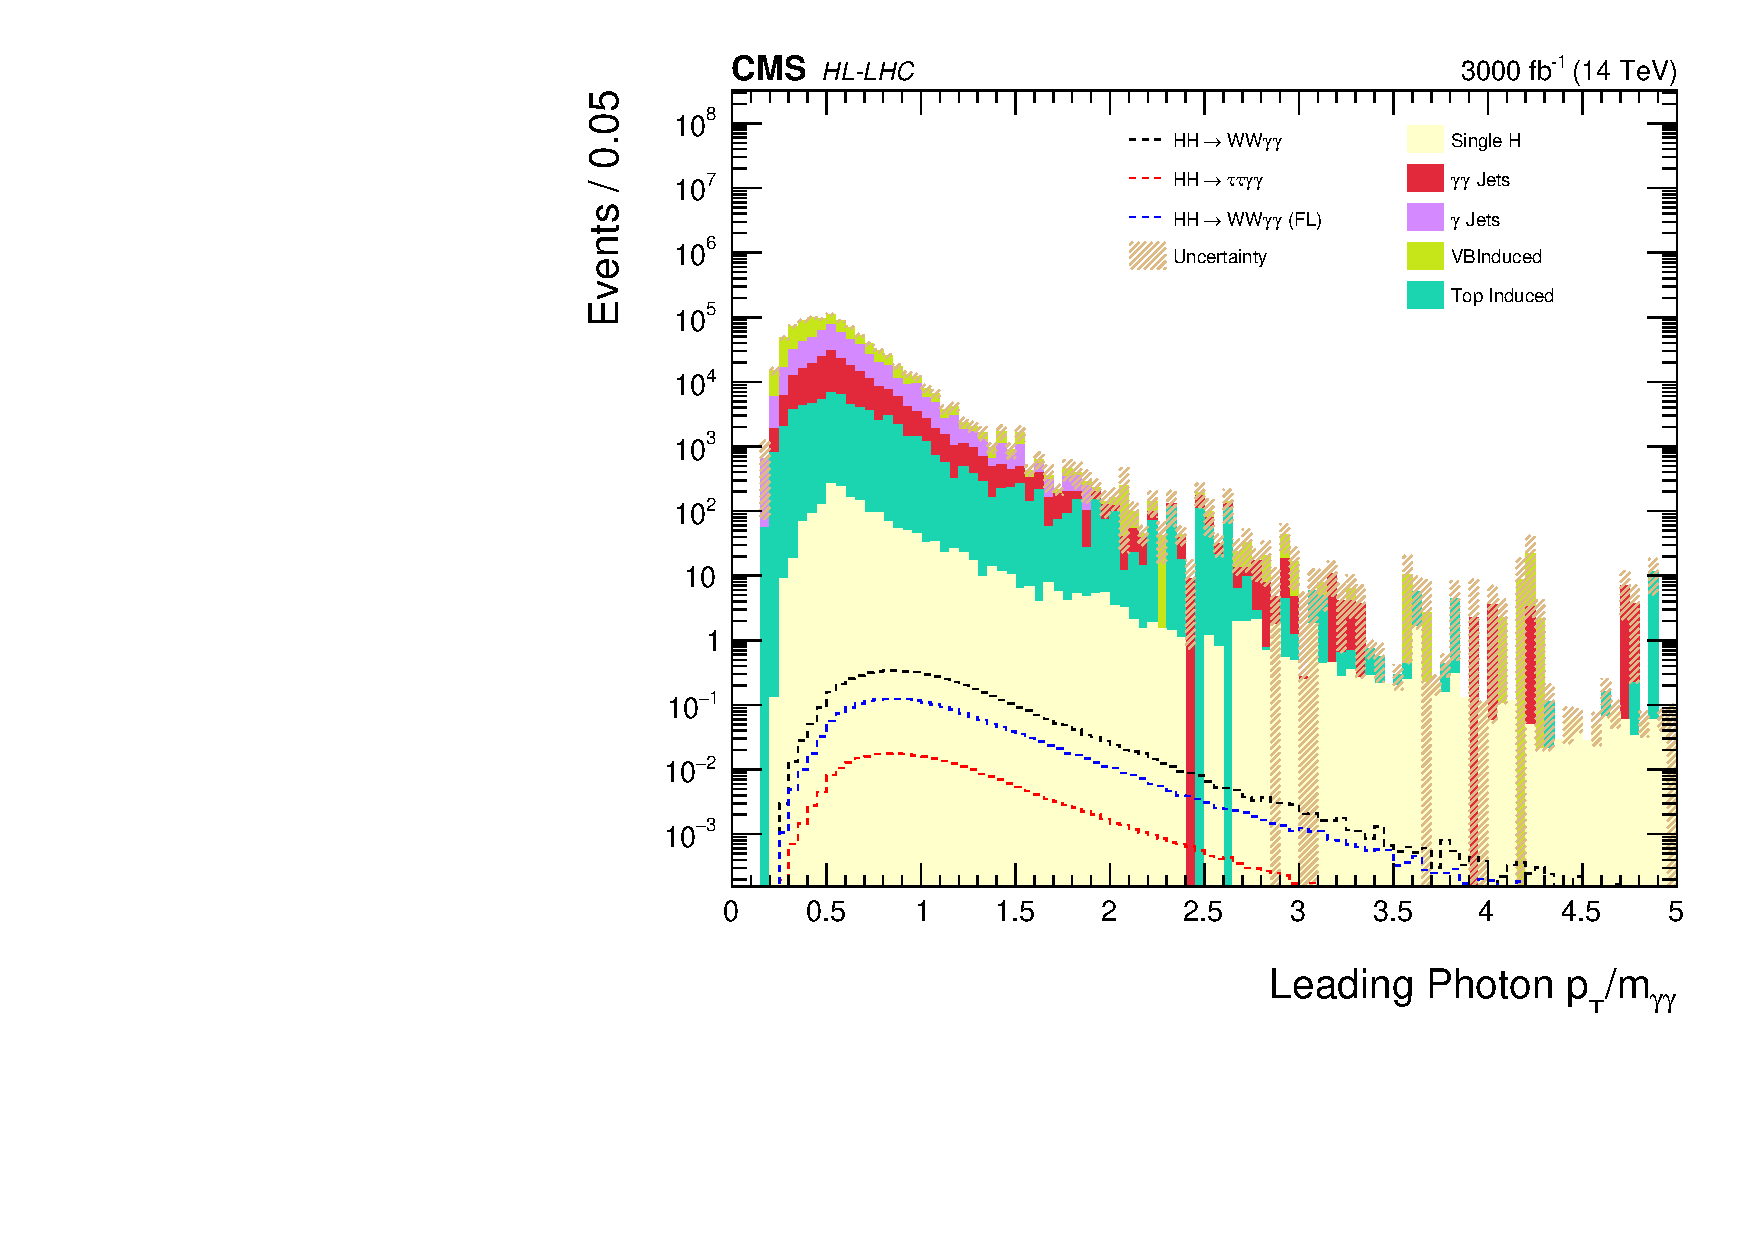
\includegraphics[width=\textwidth]{LeadingPhotonpT_mGGLhasOneL_logy.pdf}
        \vspace{-0.5cm}
        \firstsubcaption{Leading Photon p$_T$/\mgg}
    \end{subfigure}
    \hfill
    \begin{subfigure}[b]{0.475\textwidth}  
        \centering 
        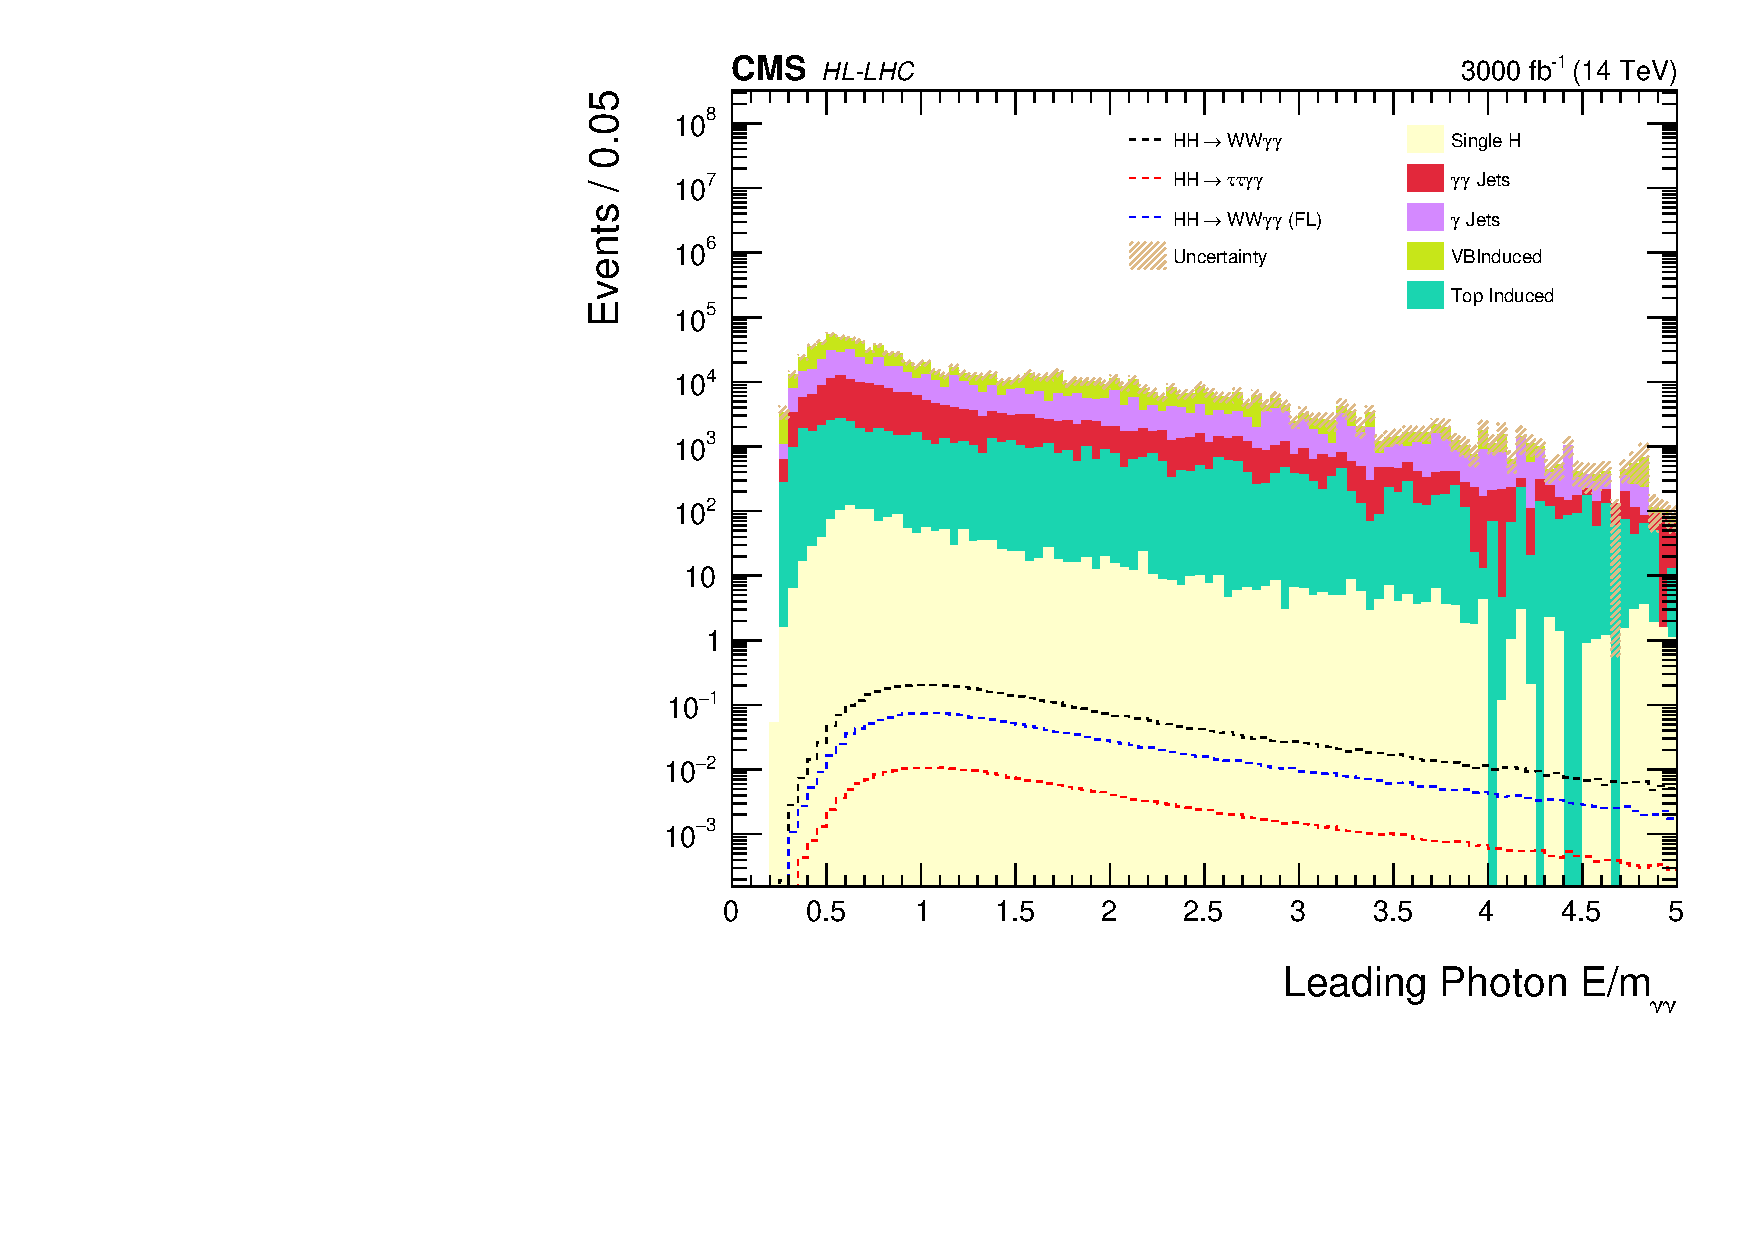
\includegraphics[width=\textwidth]{LeadingPhotonE_mGGLhasOneL_logy.pdf}
        \vspace{-0.5cm}
        \firstsubcaption{Leading Photon E/\mgg}
    \end{subfigure}
    \vskip\baselineskip
    \begin{subfigure}[b]{0.475\textwidth}   
        \centering 
        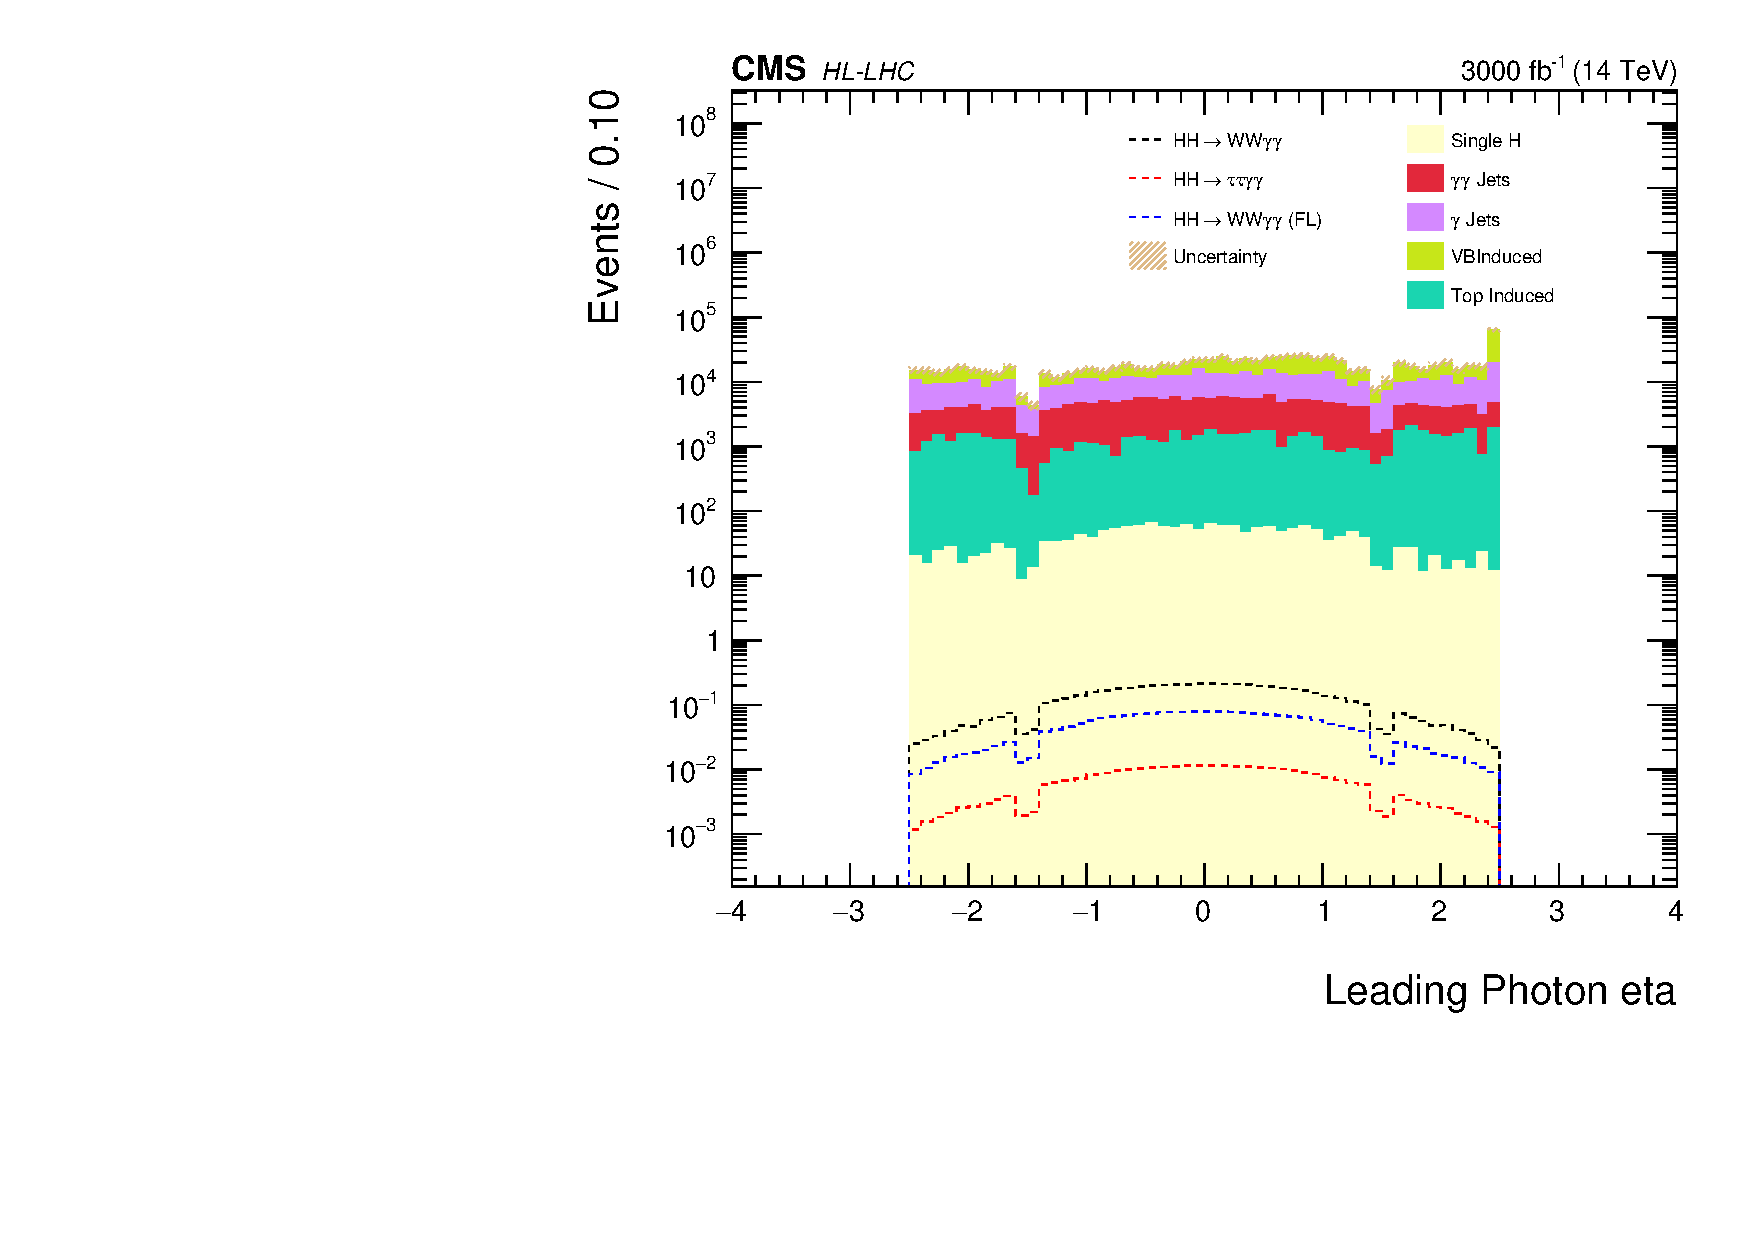
\includegraphics[width=\textwidth]{LeadingPhotonEtaOneL_logy.pdf}
        \vspace{-0.5cm}
        \firstsubcaption{Leading Photon $\eta$}
    \end{subfigure}
    \hfill
    \begin{subfigure}[b]{0.475\textwidth}   
        \centering 
        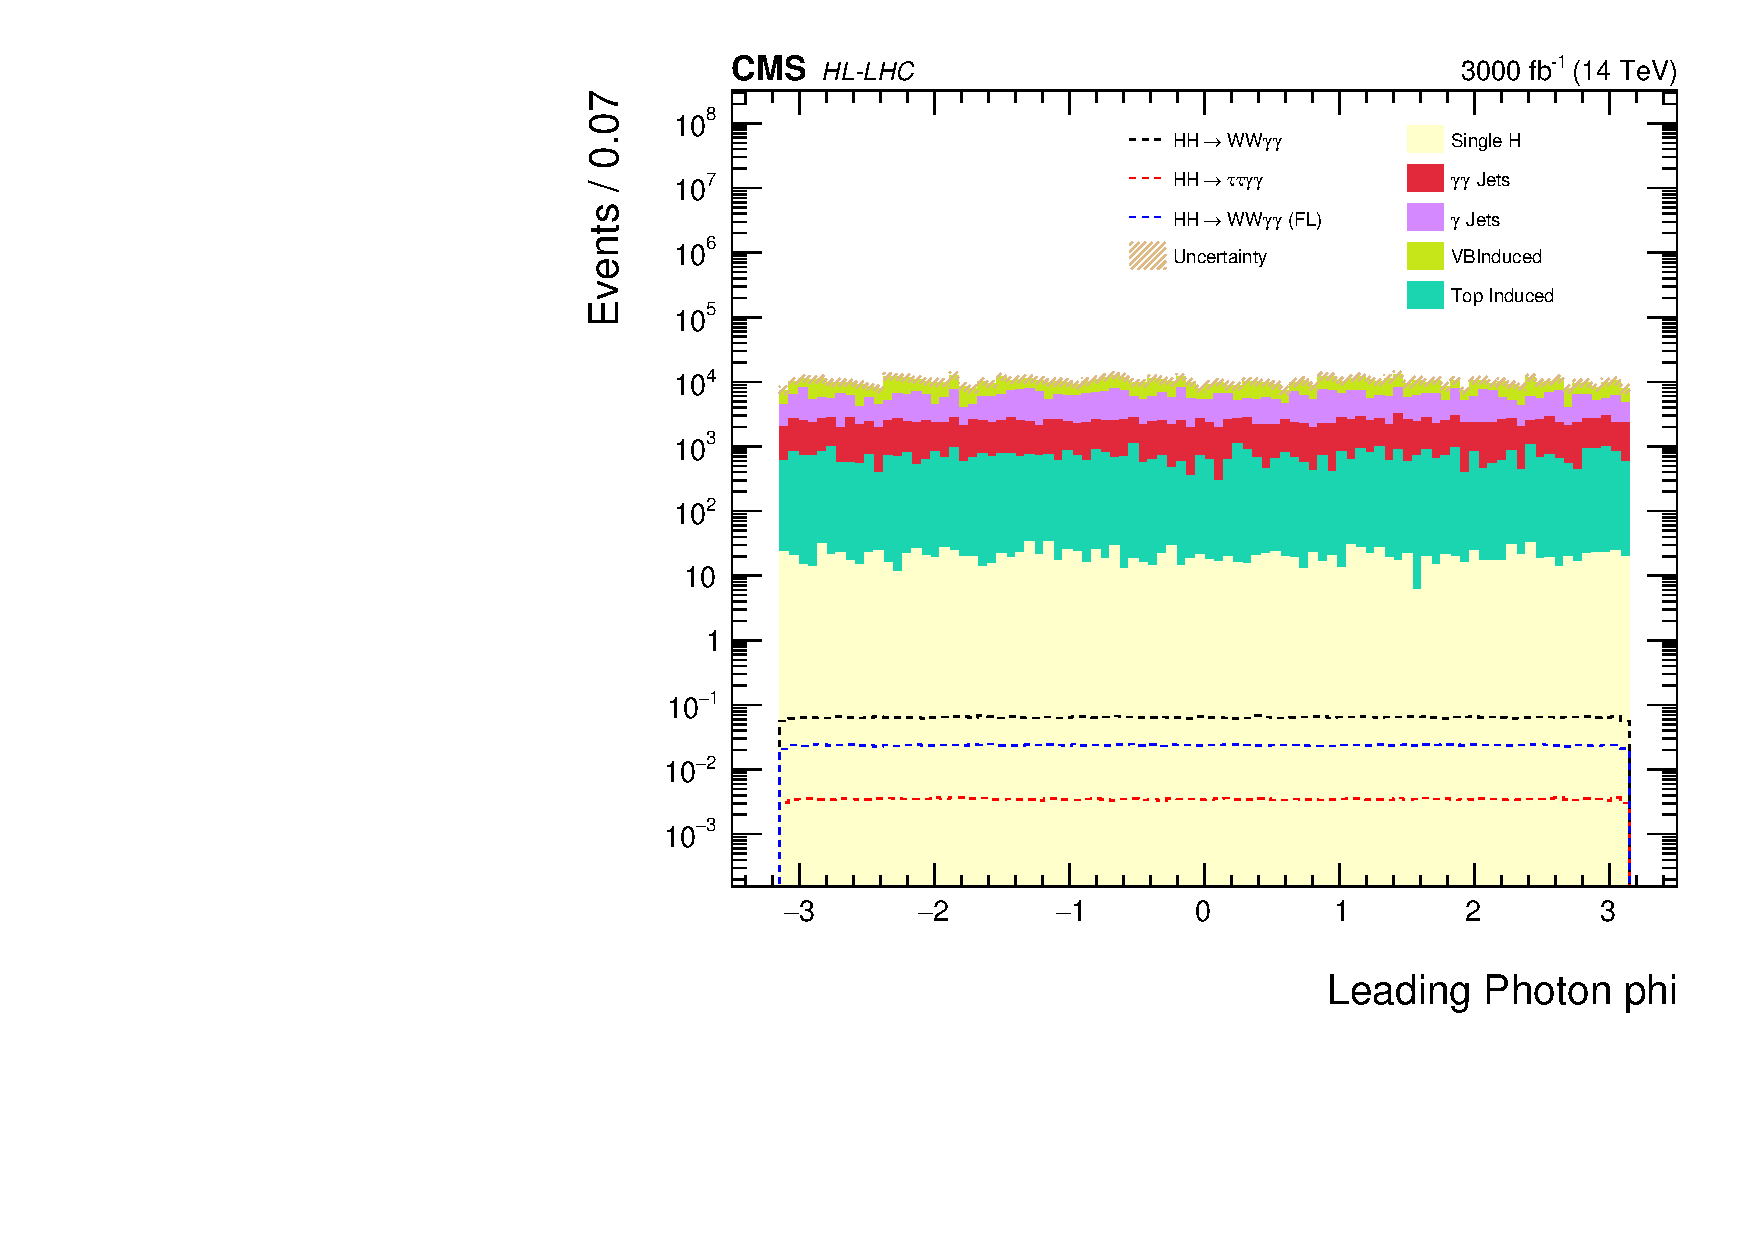
\includegraphics[width=\textwidth]{LeadingPhotonPhiOneL_logy.pdf}
        \vspace{-0.5cm}
        \firstsubcaption{Leading Photon $\phi$}
    \end{subfigure}
    \vskip\baselineskip
    \begin{subfigure}[b]{0.475\textwidth}   
        \centering 
        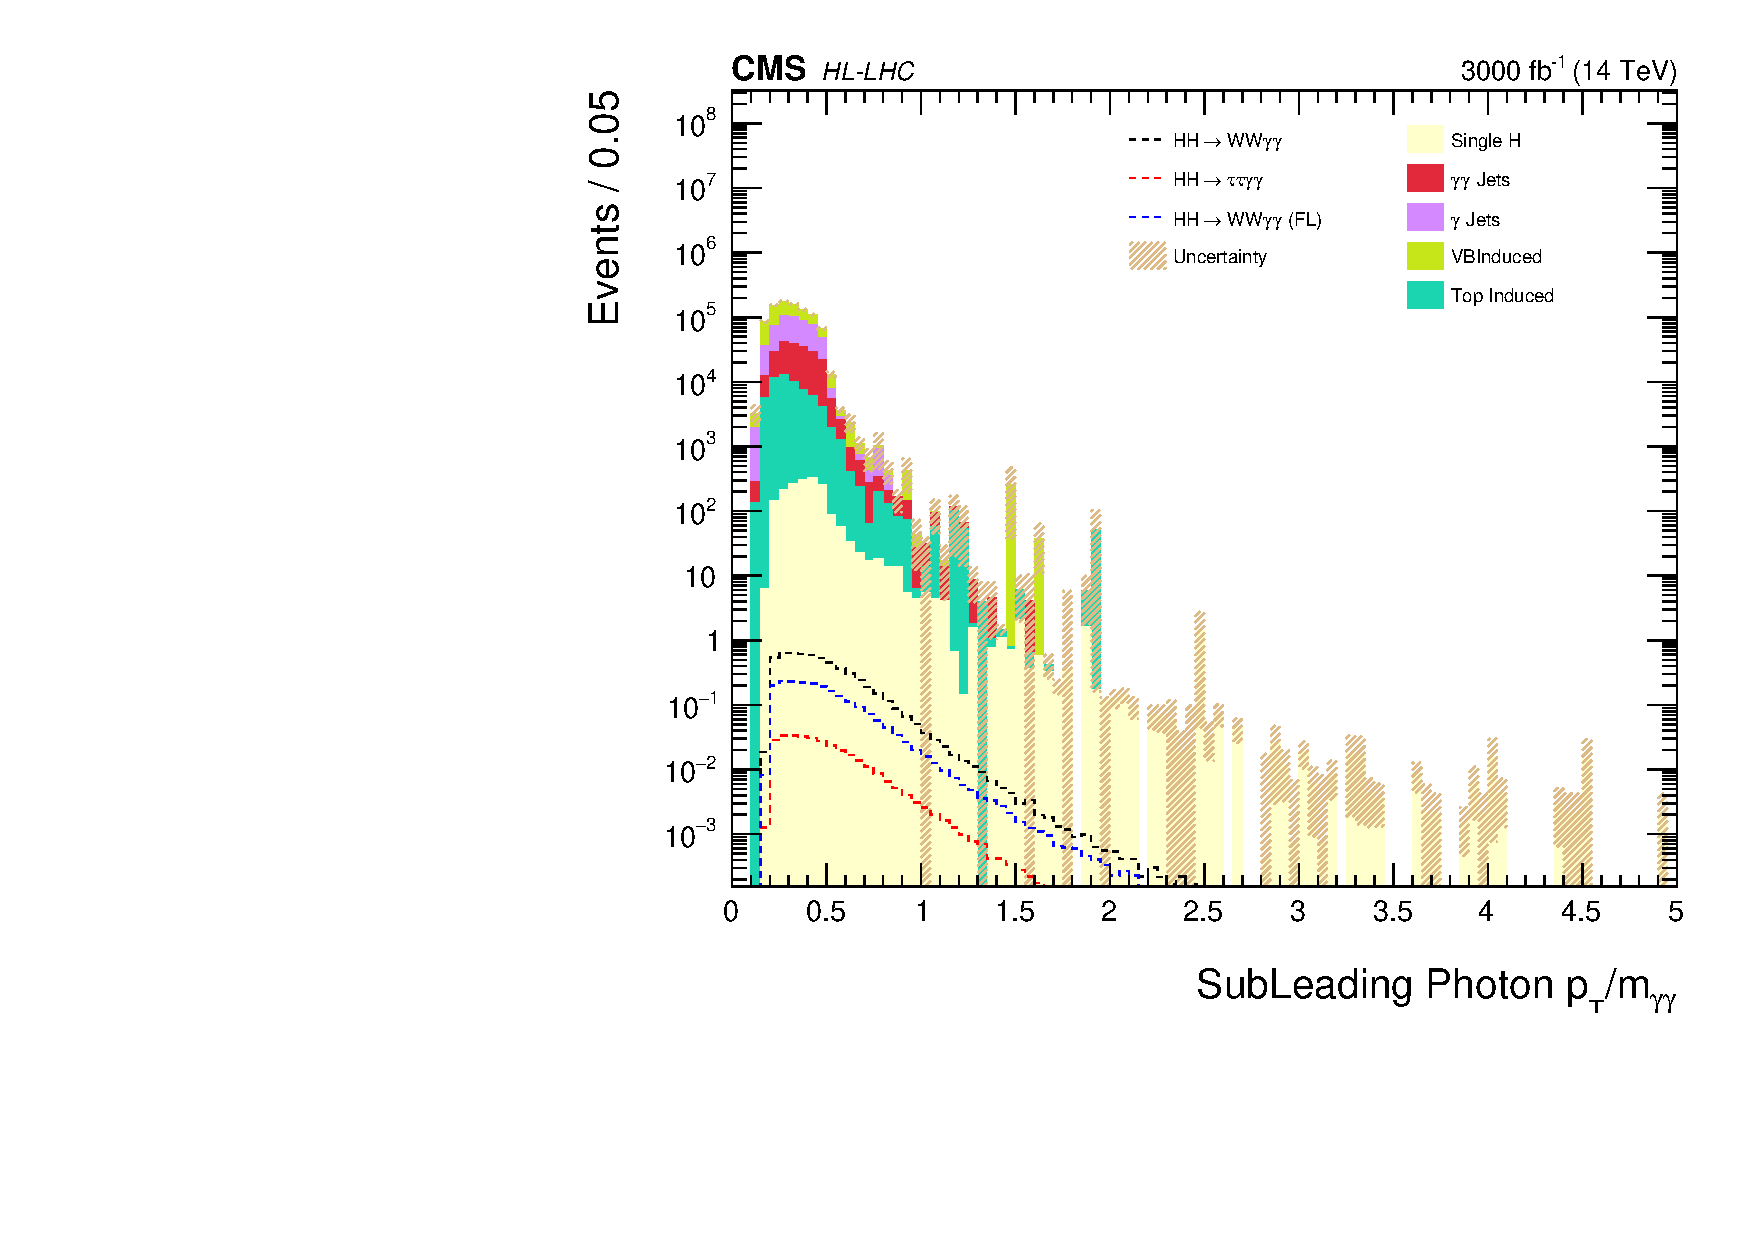
\includegraphics[width=\textwidth]{SubLeadingPhotonpT_mGGLhasOneL_logy.pdf}
        \vspace{-0.5cm}
        \firstsubcaption{Sub-leading Photon p$_T$/\mgg}
    \end{subfigure}
    \hfill
    \begin{subfigure}[b]{0.475\textwidth}   
        \centering 
        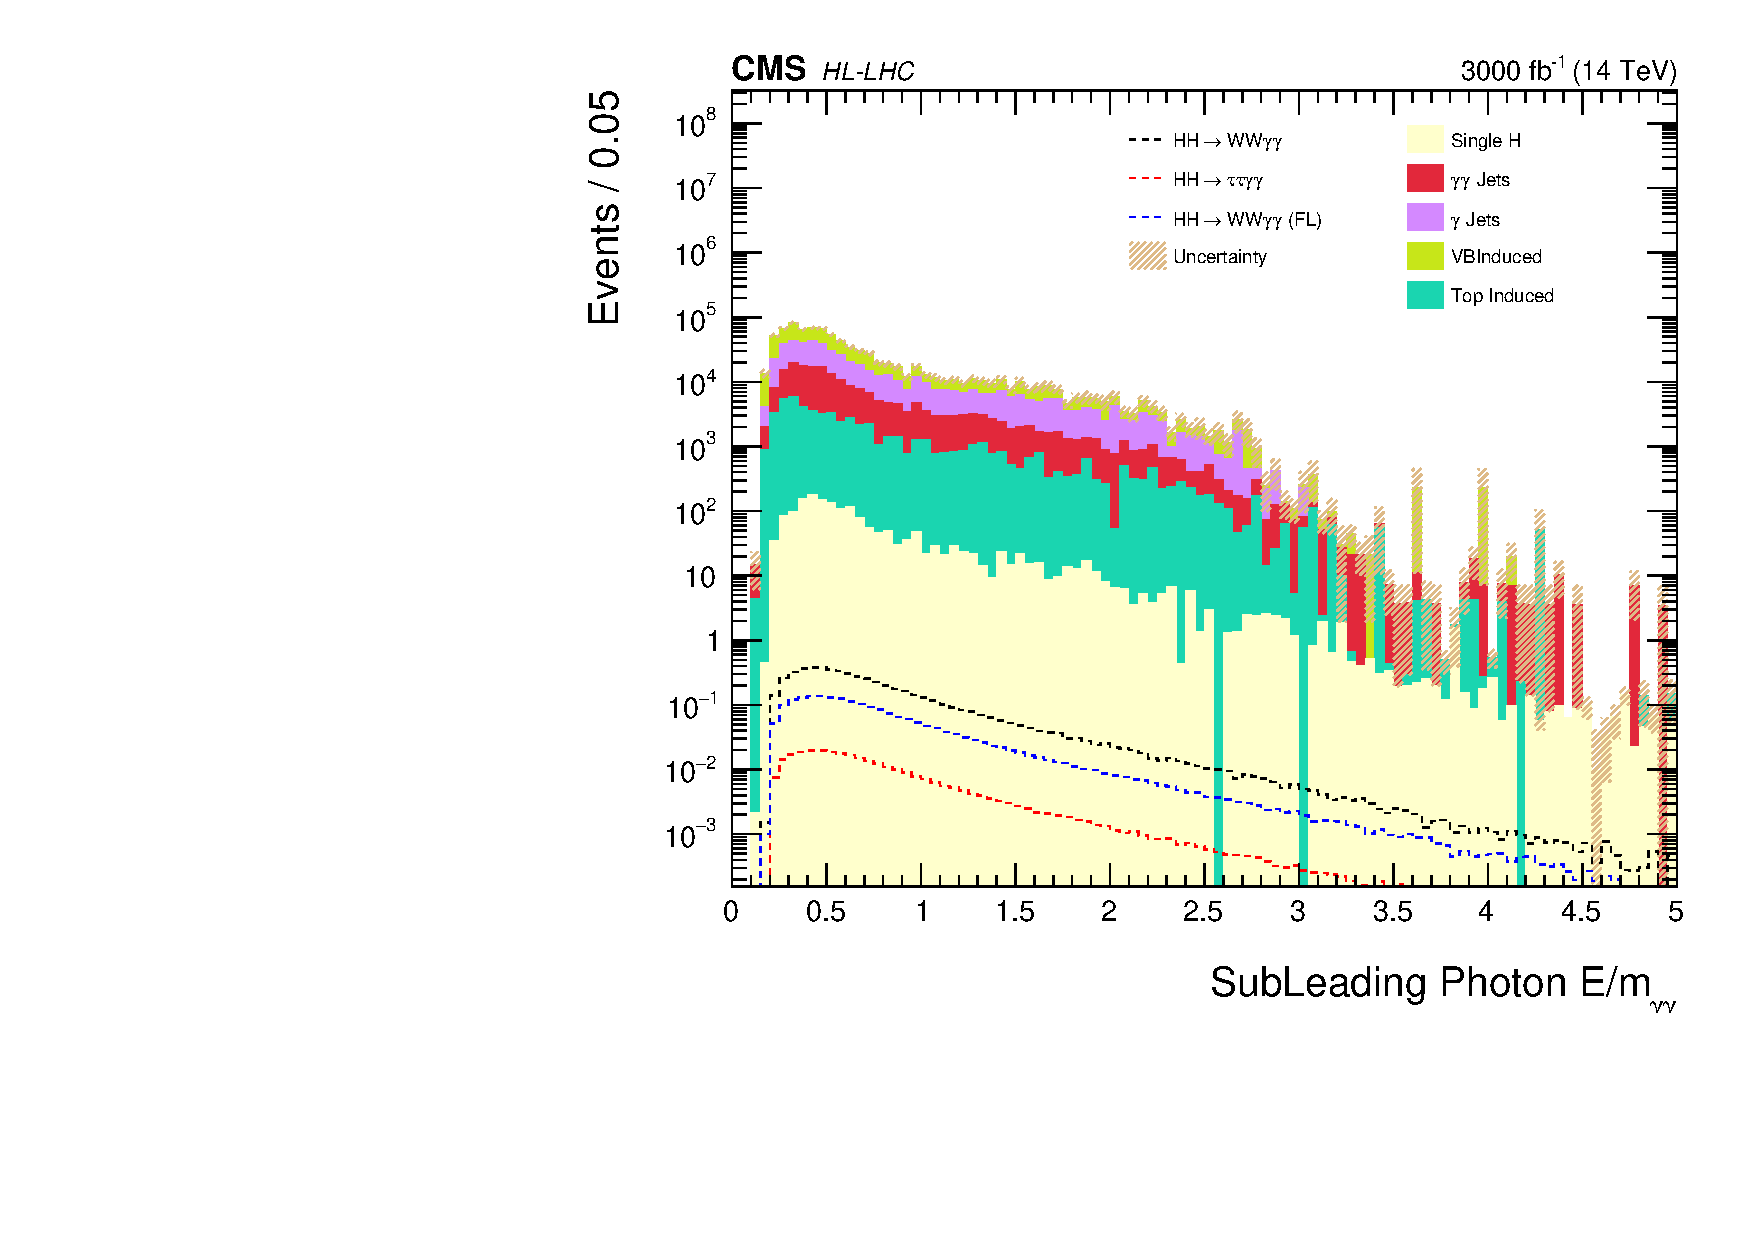
\includegraphics[width=\textwidth]{SubLeadingPhotonE_mGGLhasOneL_logy.pdf}
        \vspace{-0.5cm}
        \firstsubcaption{Sub-leading Photon E/\mgg}   
    \end{subfigure}
    \caption{\small DNN input distributions for the semi-leptonic final state.} 
    \label{hasOneL_plots}
\end{figure*}
\newpage

\begin{figure*}[h!]
    \centering
    \begin{subfigure}[b]{0.475\textwidth}
        \centering
        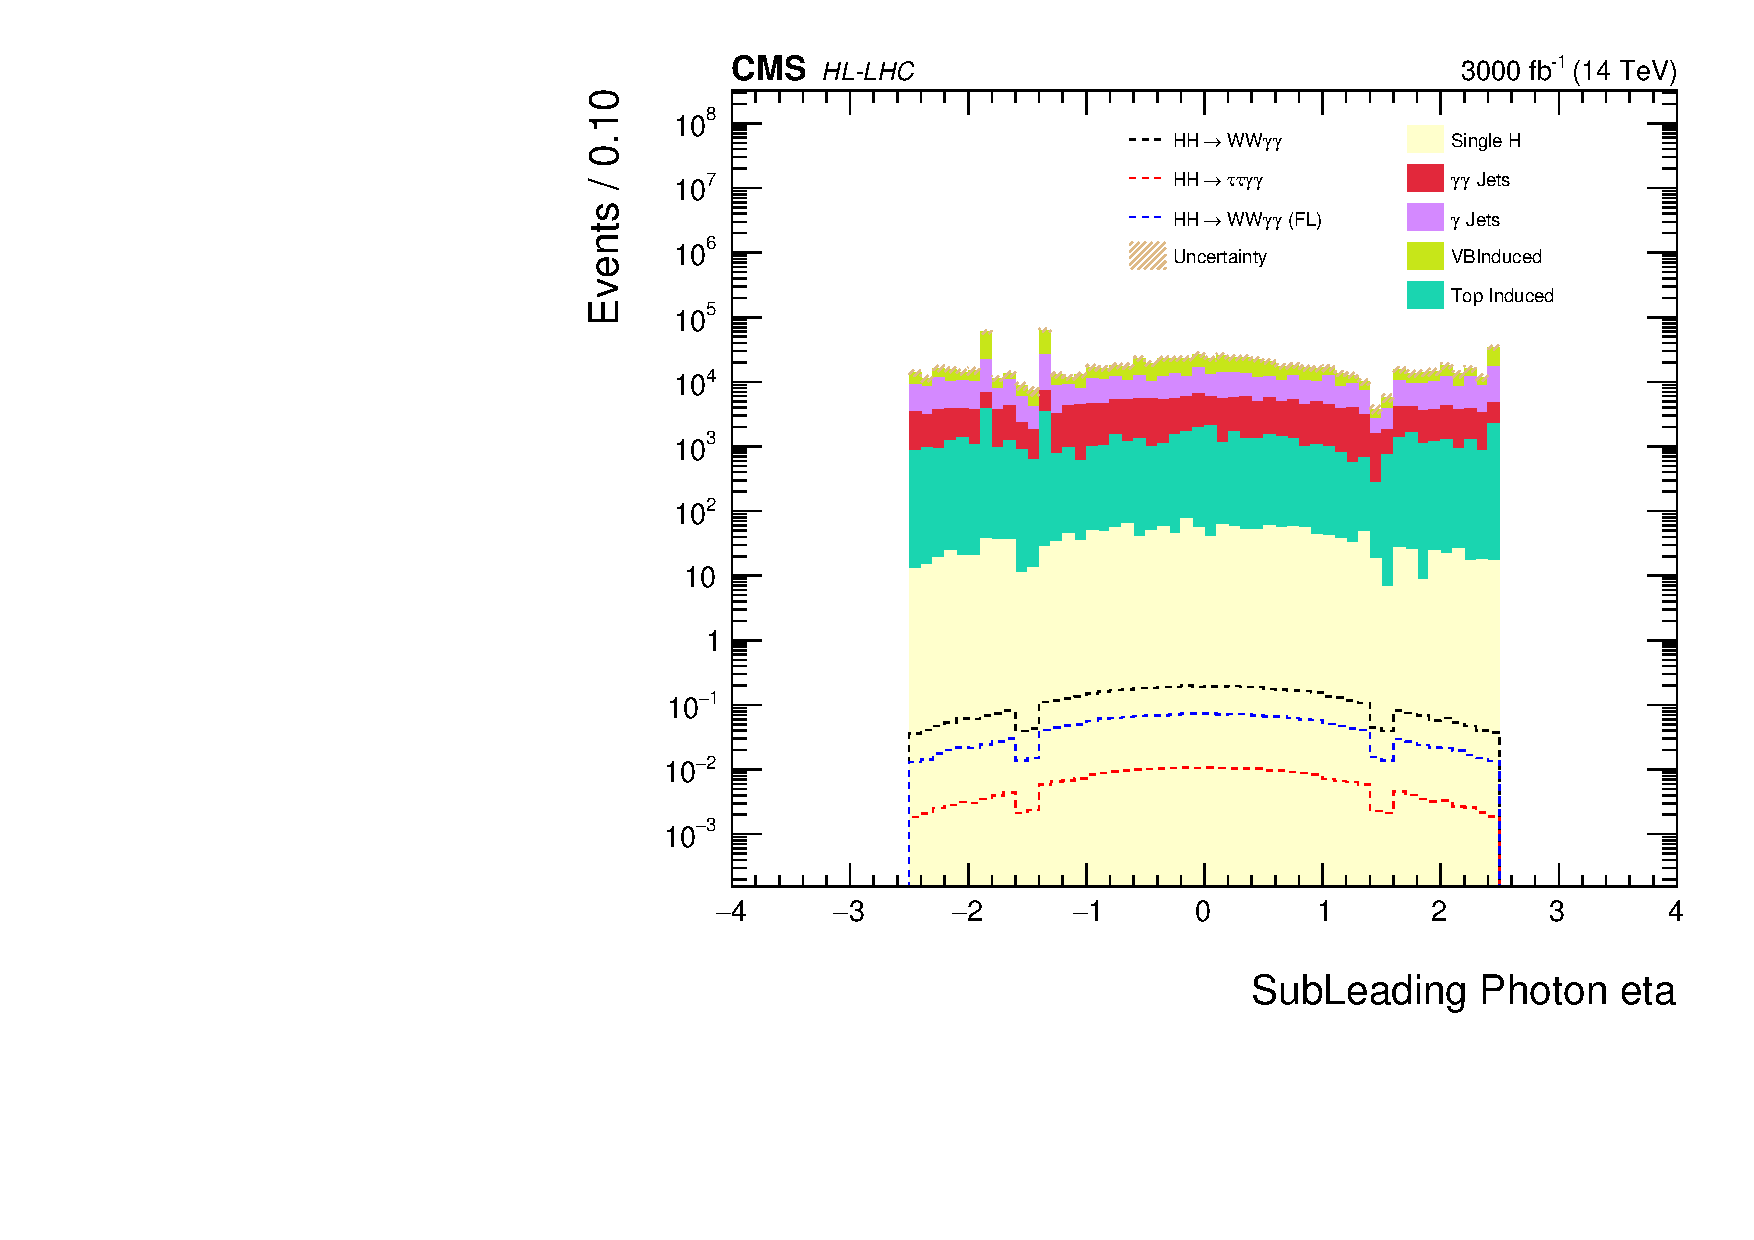
\includegraphics[width=\textwidth]{SubLeadingPhotonEtaOneL_logy.pdf}
        \vspace{-0.5cm}
        \firstsubcaption{Sub-leading Photon $\eta$}
    \end{subfigure}
    \hfill
    \begin{subfigure}[b]{0.475\textwidth}  
        \centering 
        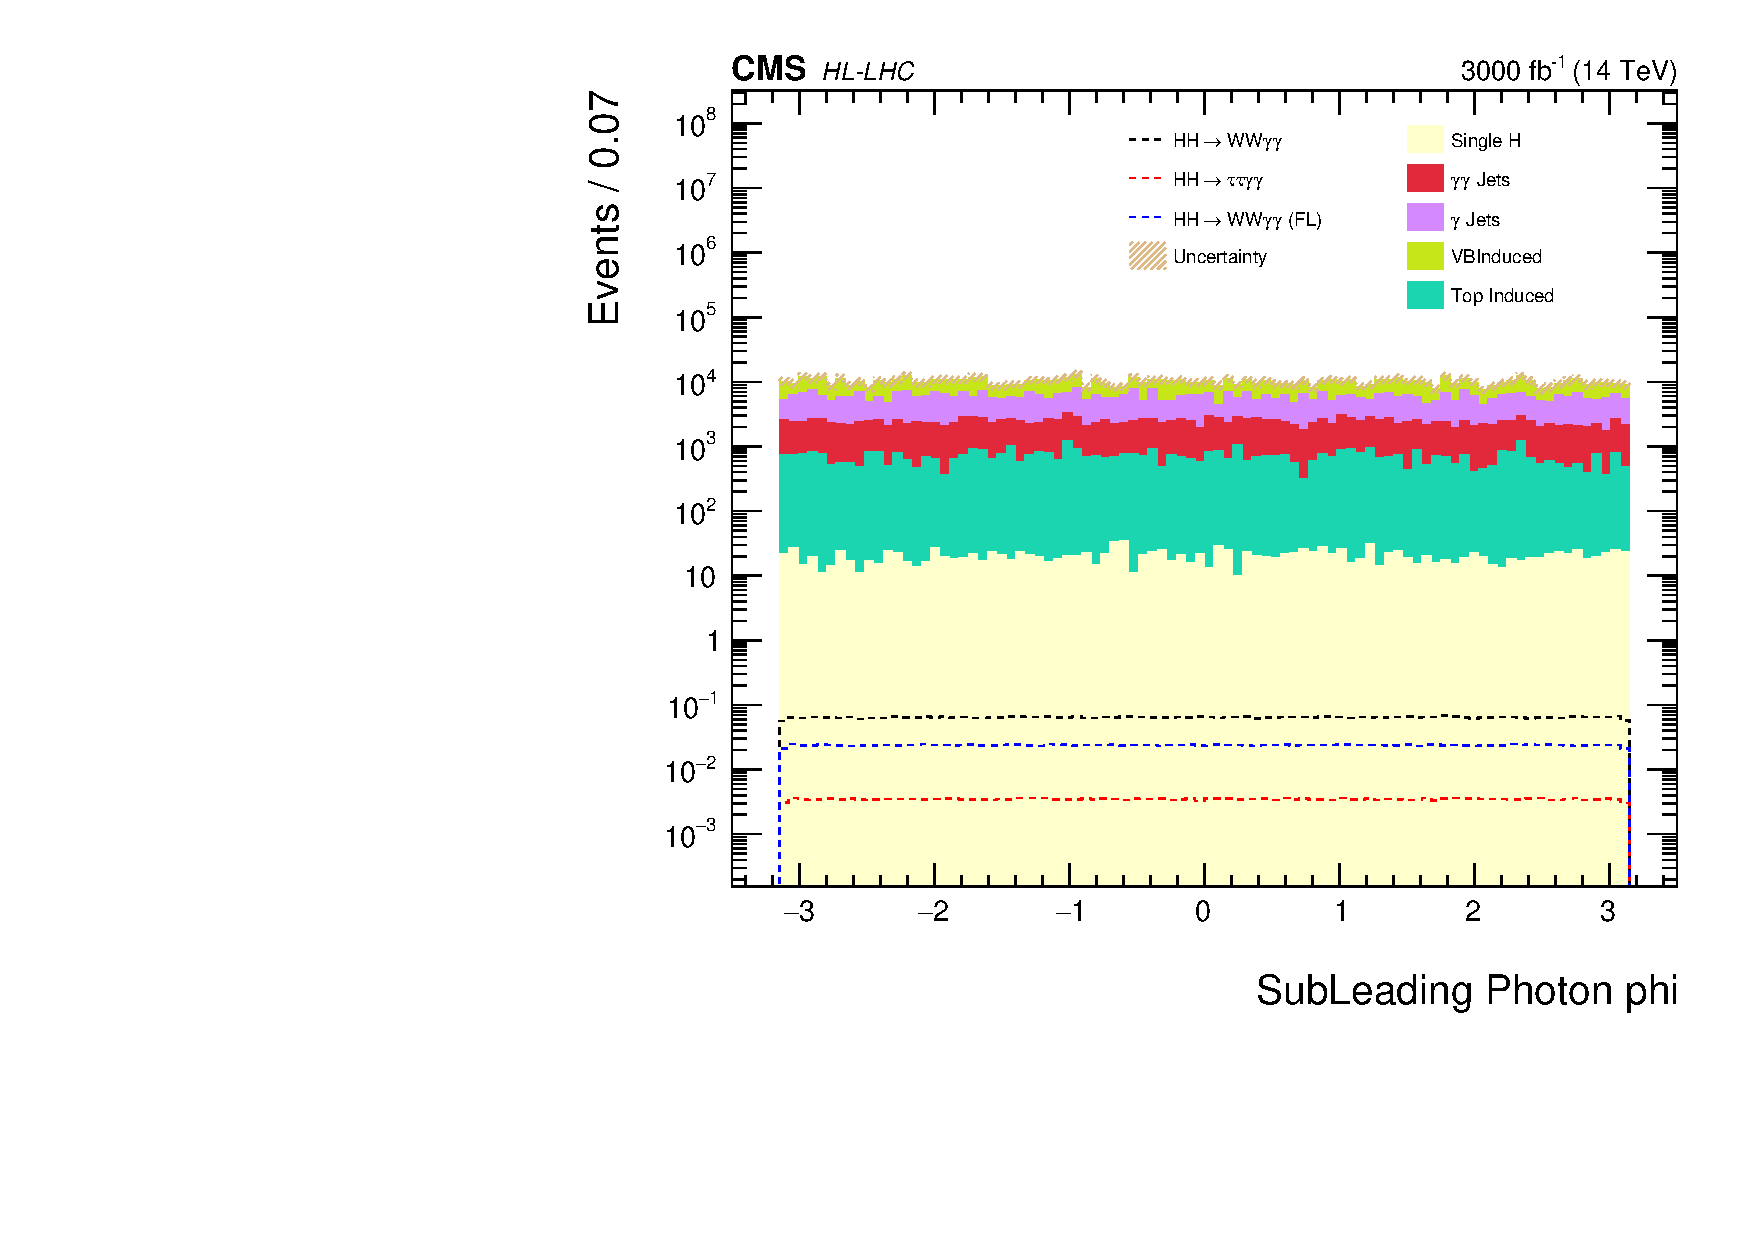
\includegraphics[width=\textwidth]{SubLeadingPhotonPhiOneL_logy.pdf}
        \vspace{-0.5cm}
        \firstsubcaption{Sub-leading Photon $\phi$}
    \end{subfigure}
    \vskip\baselineskip
    \begin{subfigure}[b]{0.475\textwidth}   
        \centering 
        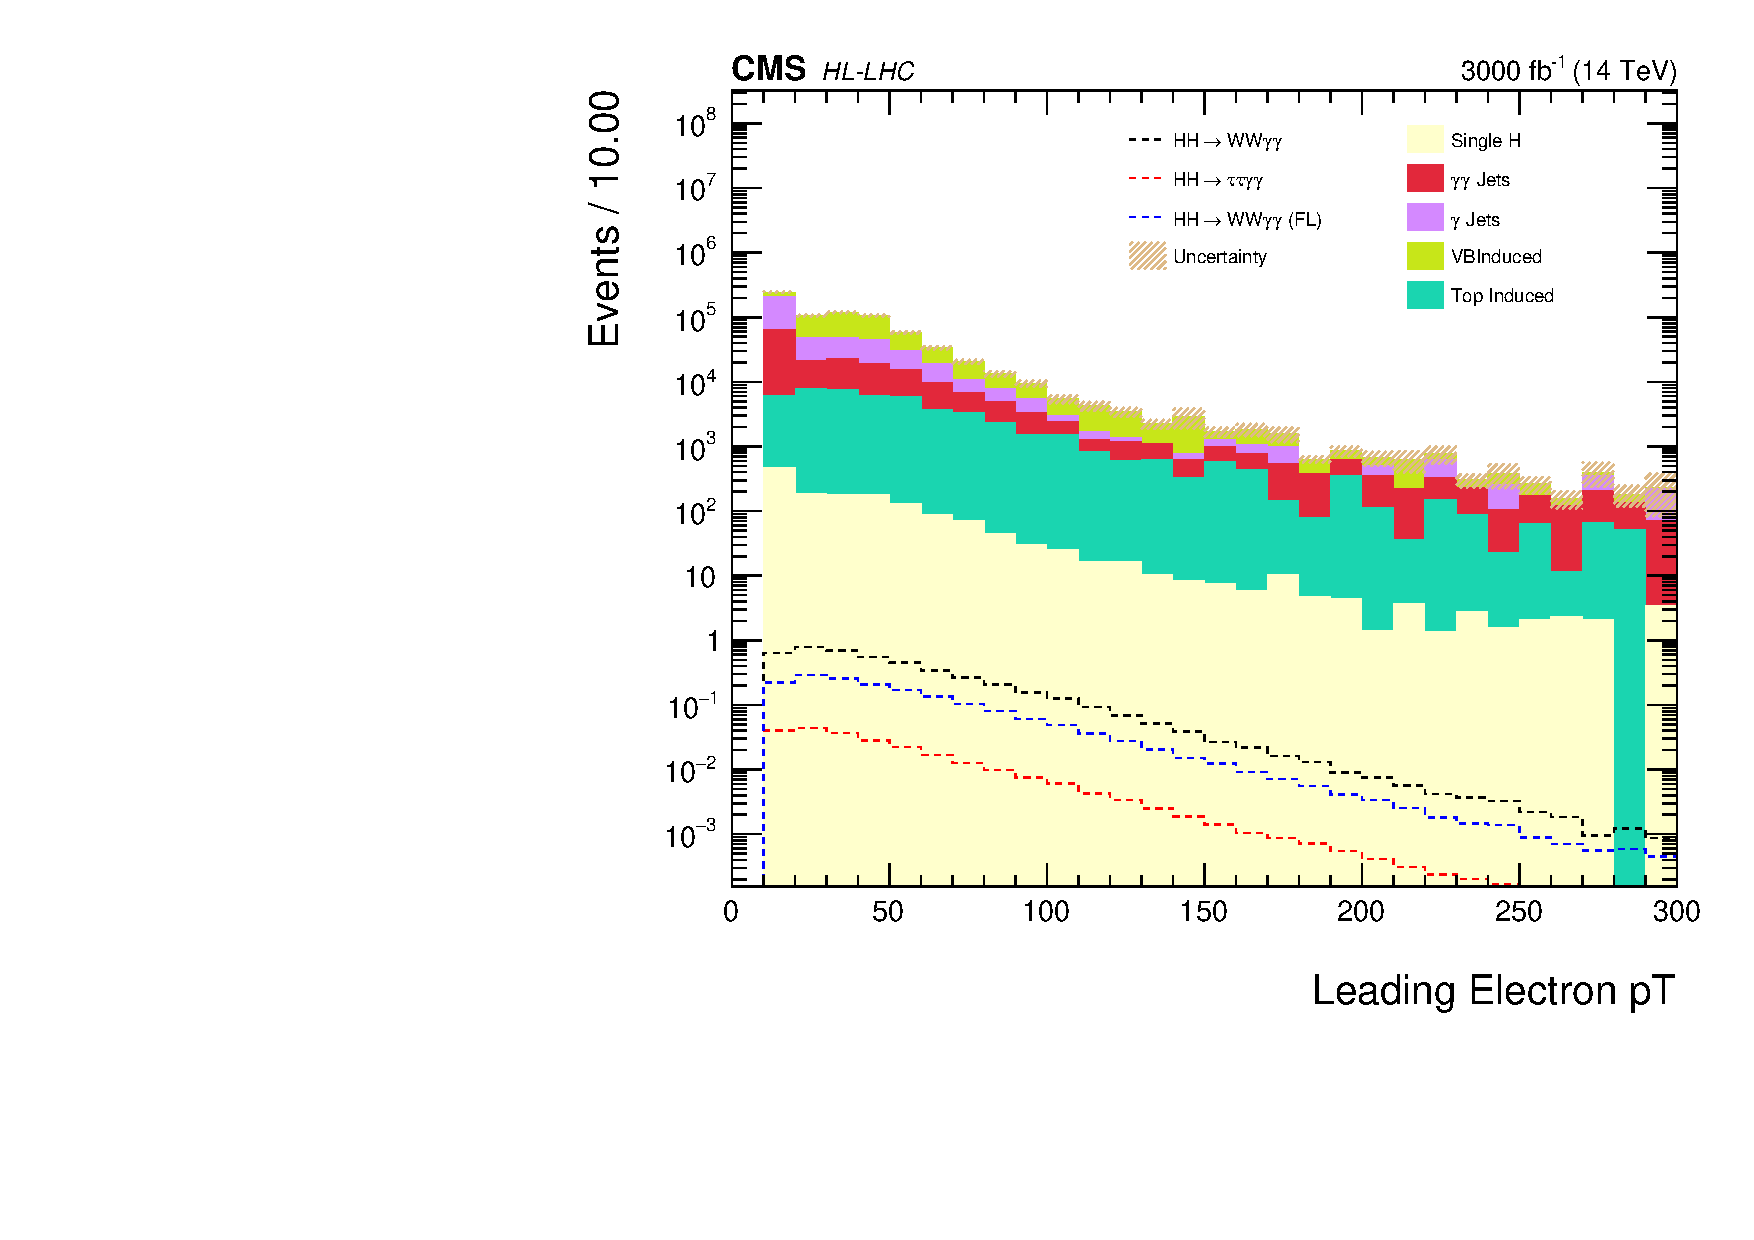
\includegraphics[width=\textwidth]{ElectronpT_logy.pdf}
        \vspace{-0.5cm}
        \firstsubcaption{Leading Electron p$_{T}$}
    \end{subfigure}
    \hfill
    \begin{subfigure}[b]{0.475\textwidth}   
        \centering 
        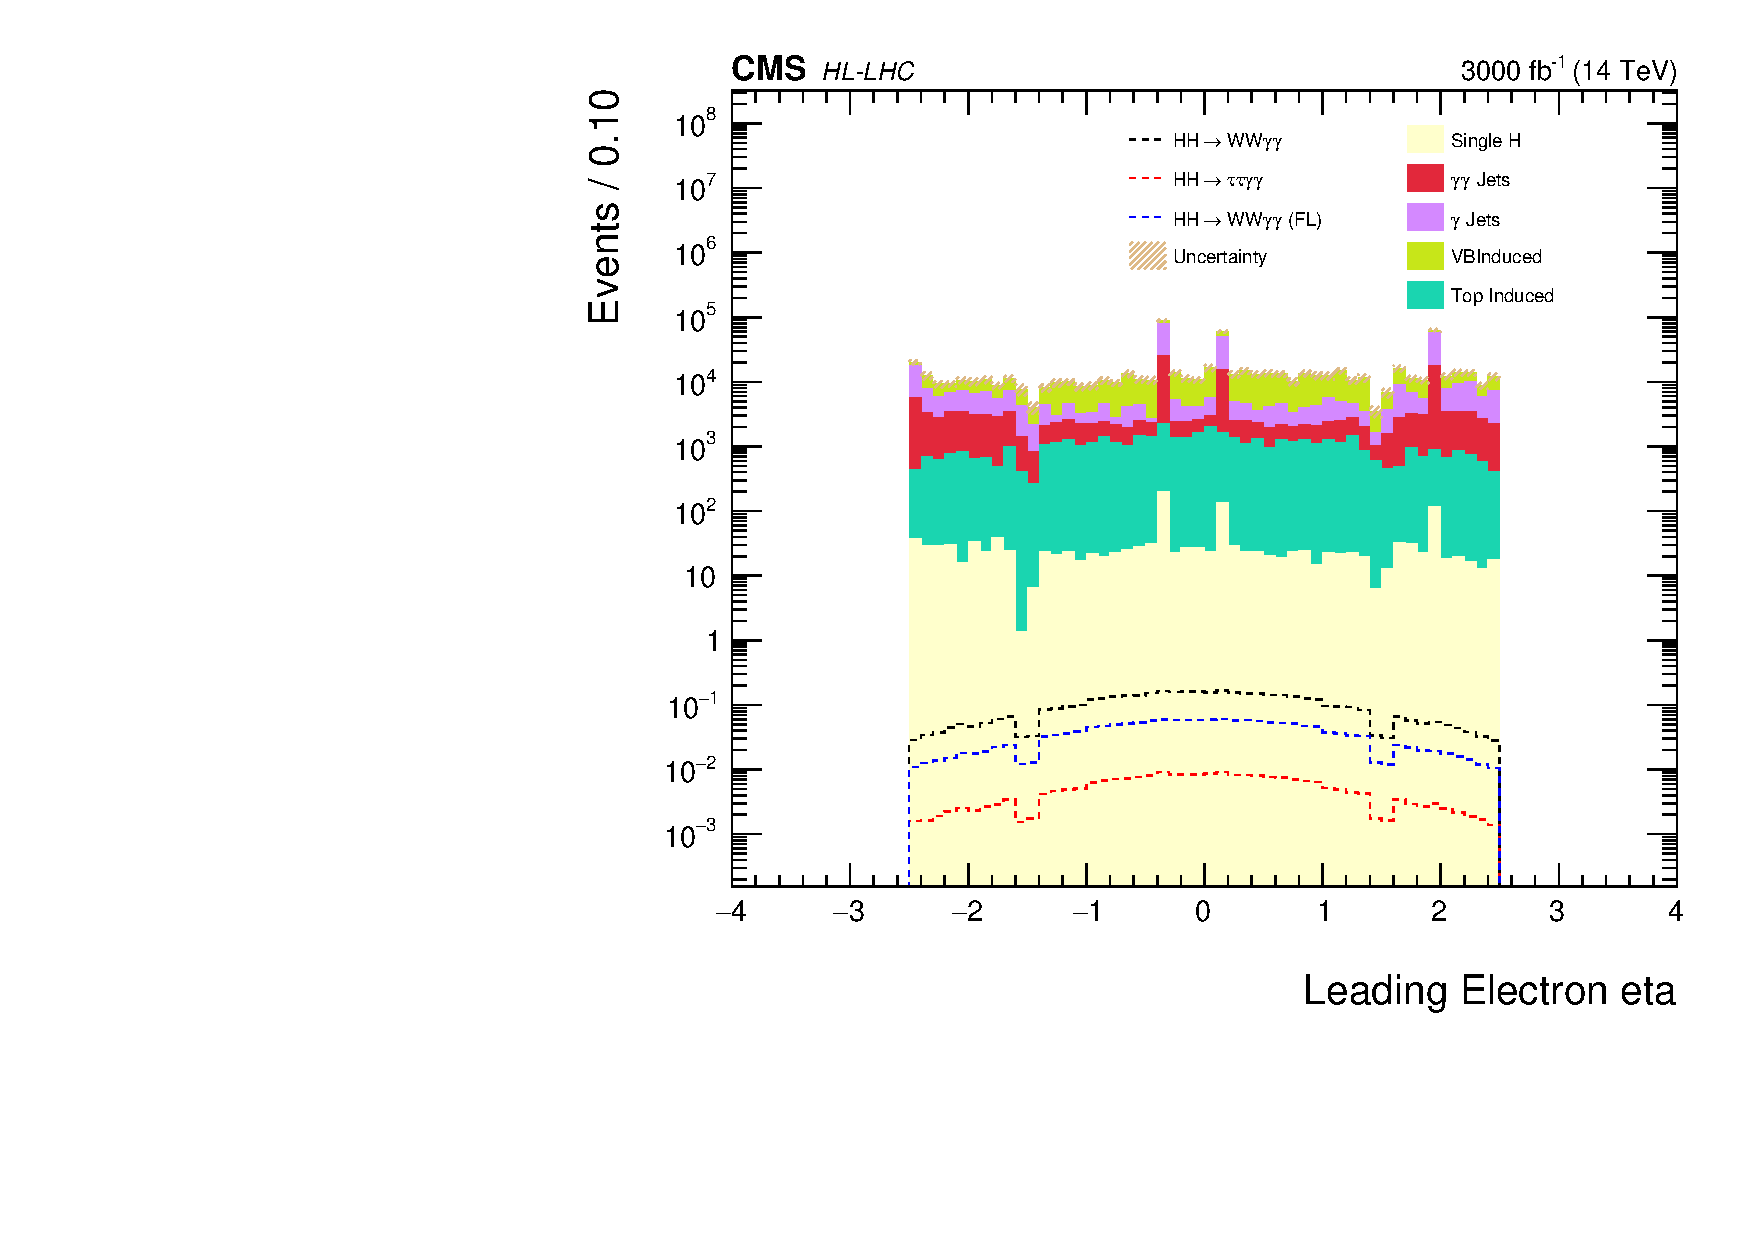
\includegraphics[width=\textwidth]{ElectronEta_logy.pdf}
        \vspace{-0.5cm}
        \firstsubcaption{Leading Electron $\eta$}
    \end{subfigure}
    \vskip\baselineskip
    \begin{subfigure}[b]{0.475\textwidth}   
        \centering 
        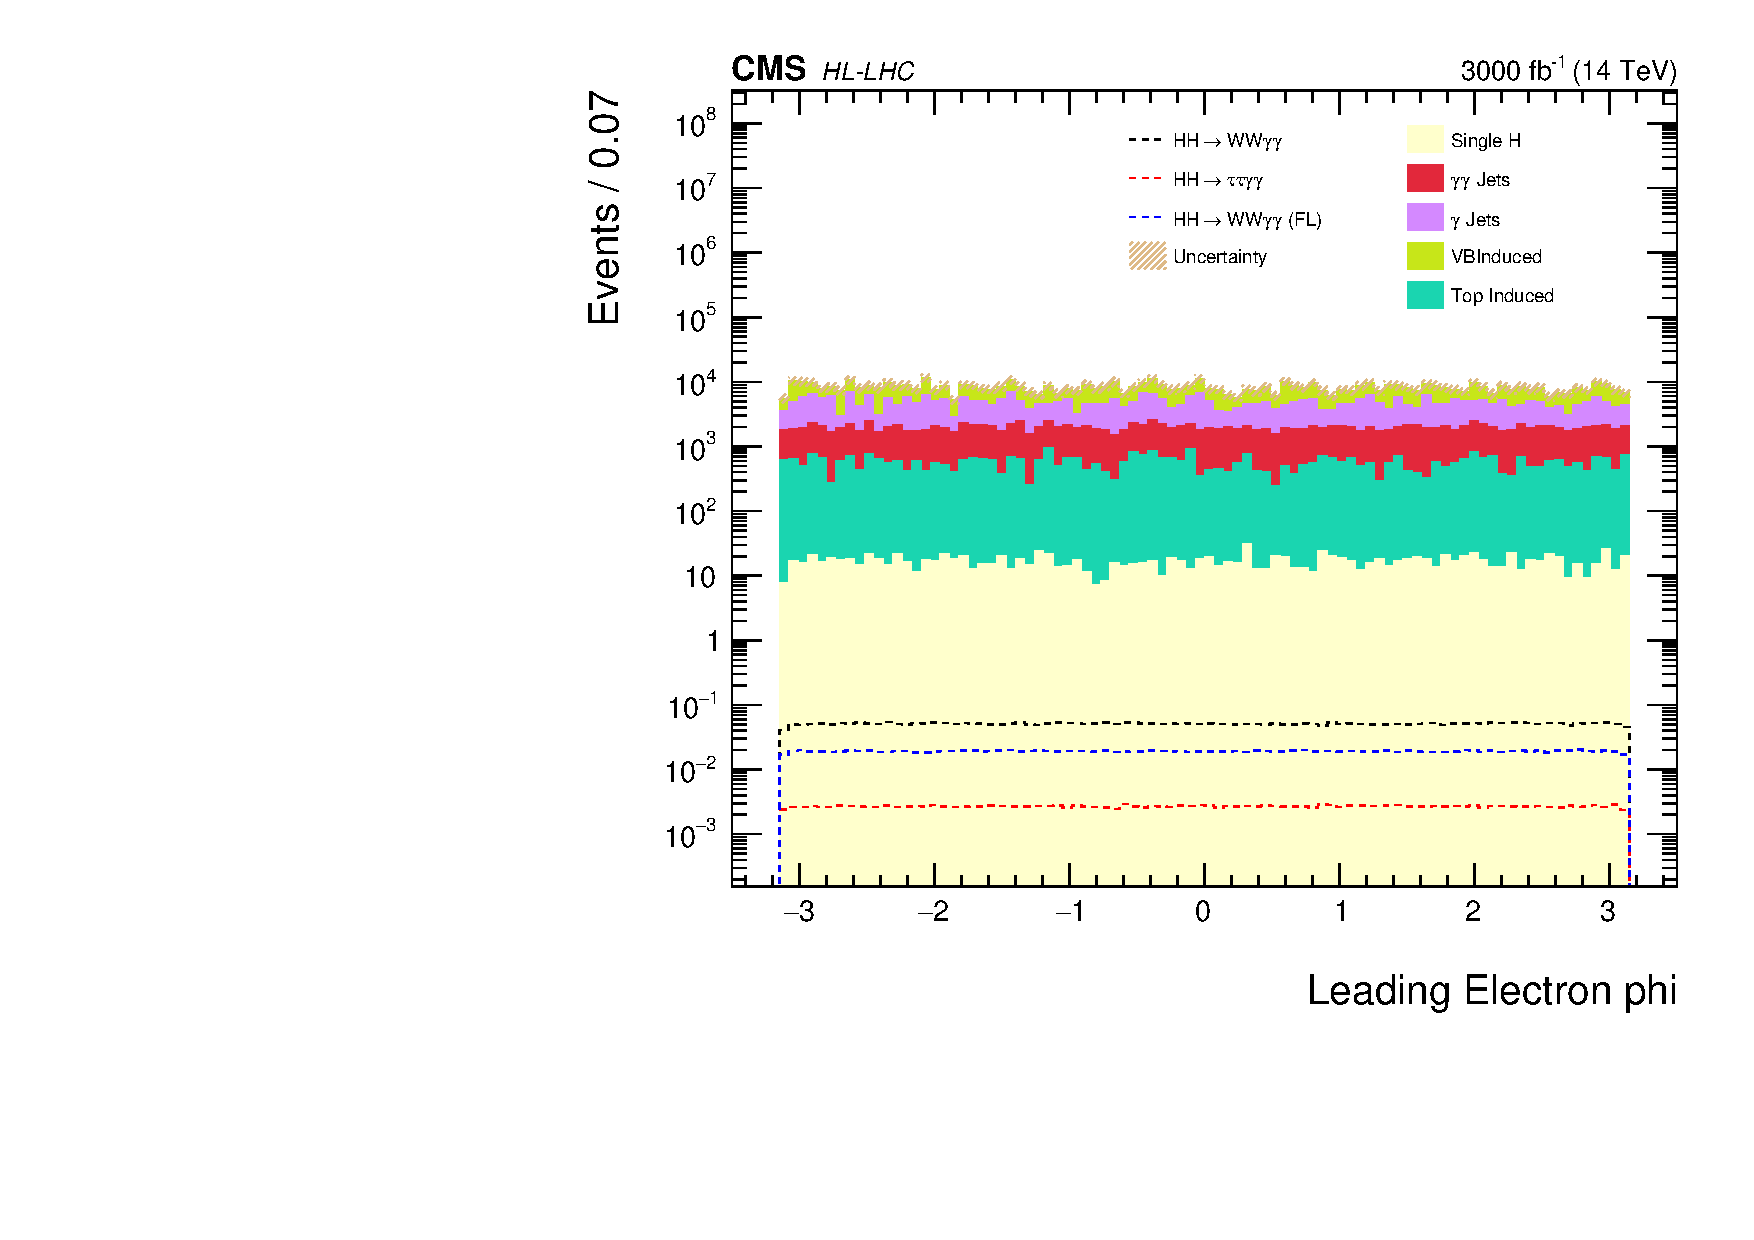
\includegraphics[width=\textwidth]{ElectronPhi_logy.pdf}
        \vspace{-0.5cm}
        \firstsubcaption{Leading Electron $\phi$}
    \end{subfigure}
    \hfill
    \begin{subfigure}[b]{0.475\textwidth}   
        \centering 
        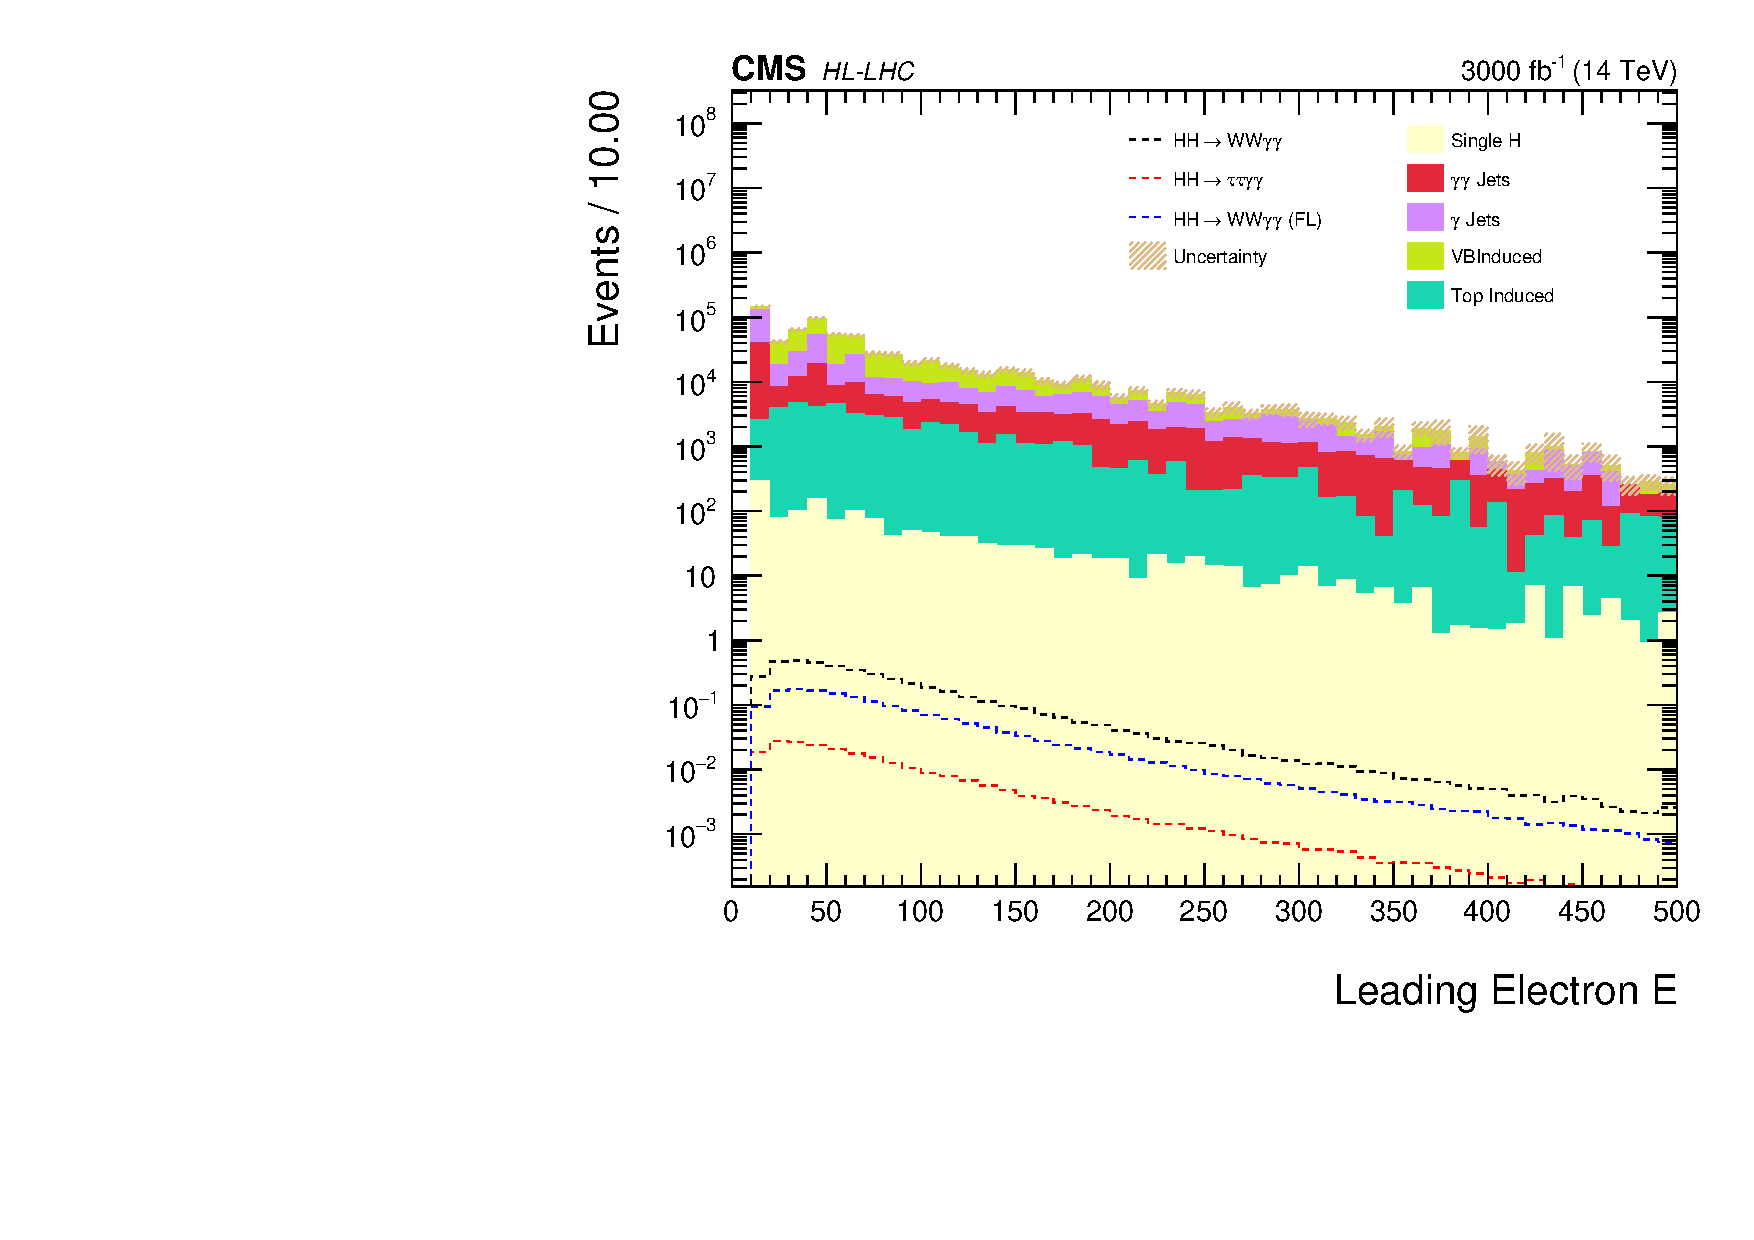
\includegraphics[width=\textwidth]{ElectronE_logy.pdf}
        \vspace{-0.5cm}
        \firstsubcaption{Leading Electron energy}   
    \end{subfigure}
    \caption{\small DNN input distributions for the semi-leptonic final state (continued).}
\end{figure*}
\newpage

\begin{figure*}[h!]
    \centering
    \begin{subfigure}[b]{0.475\textwidth}
        \centering
        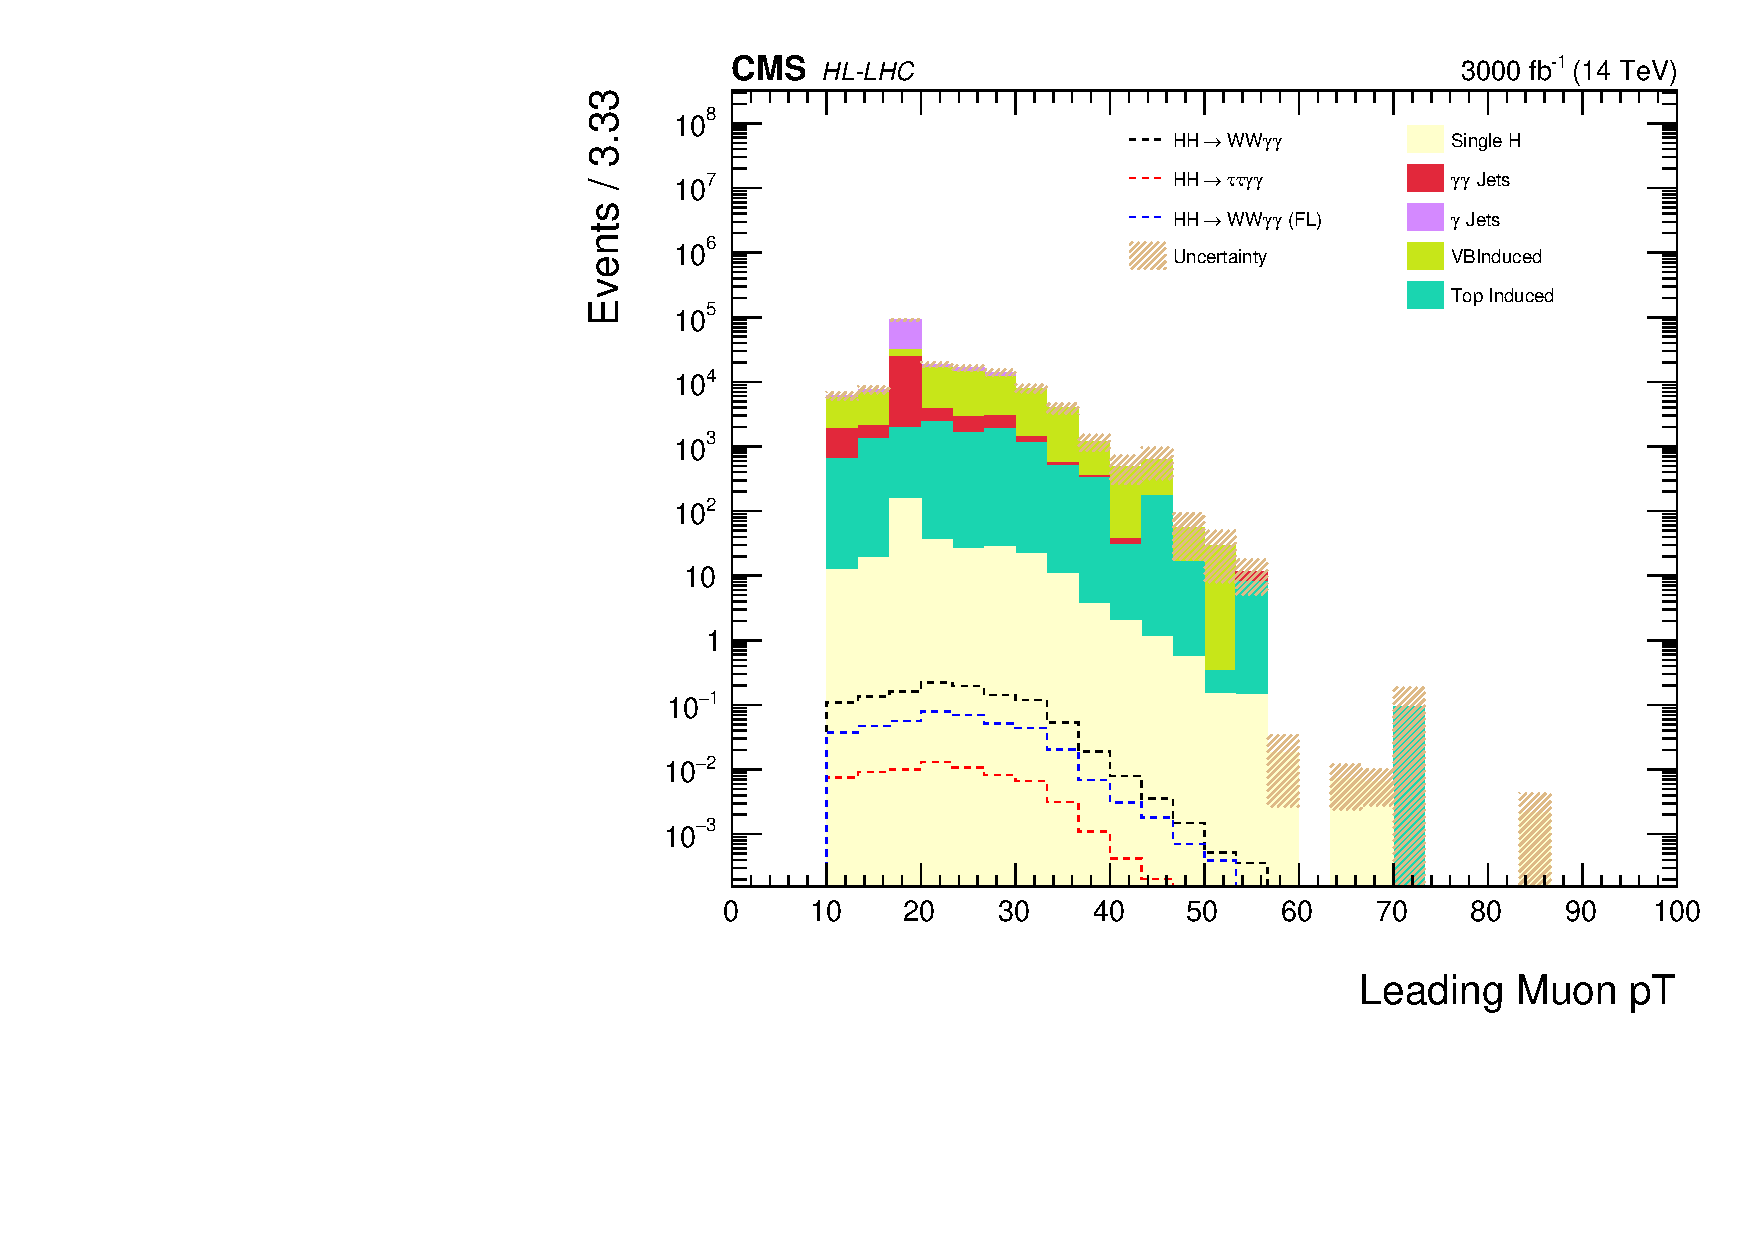
\includegraphics[width=\textwidth]{MuonpT_logy.pdf}
        \vspace{-0.5cm}
        \firstsubcaption{Leading Muon \pt}
    \end{subfigure}
    \hfill
    \begin{subfigure}[b]{0.475\textwidth}  
        \centering 
        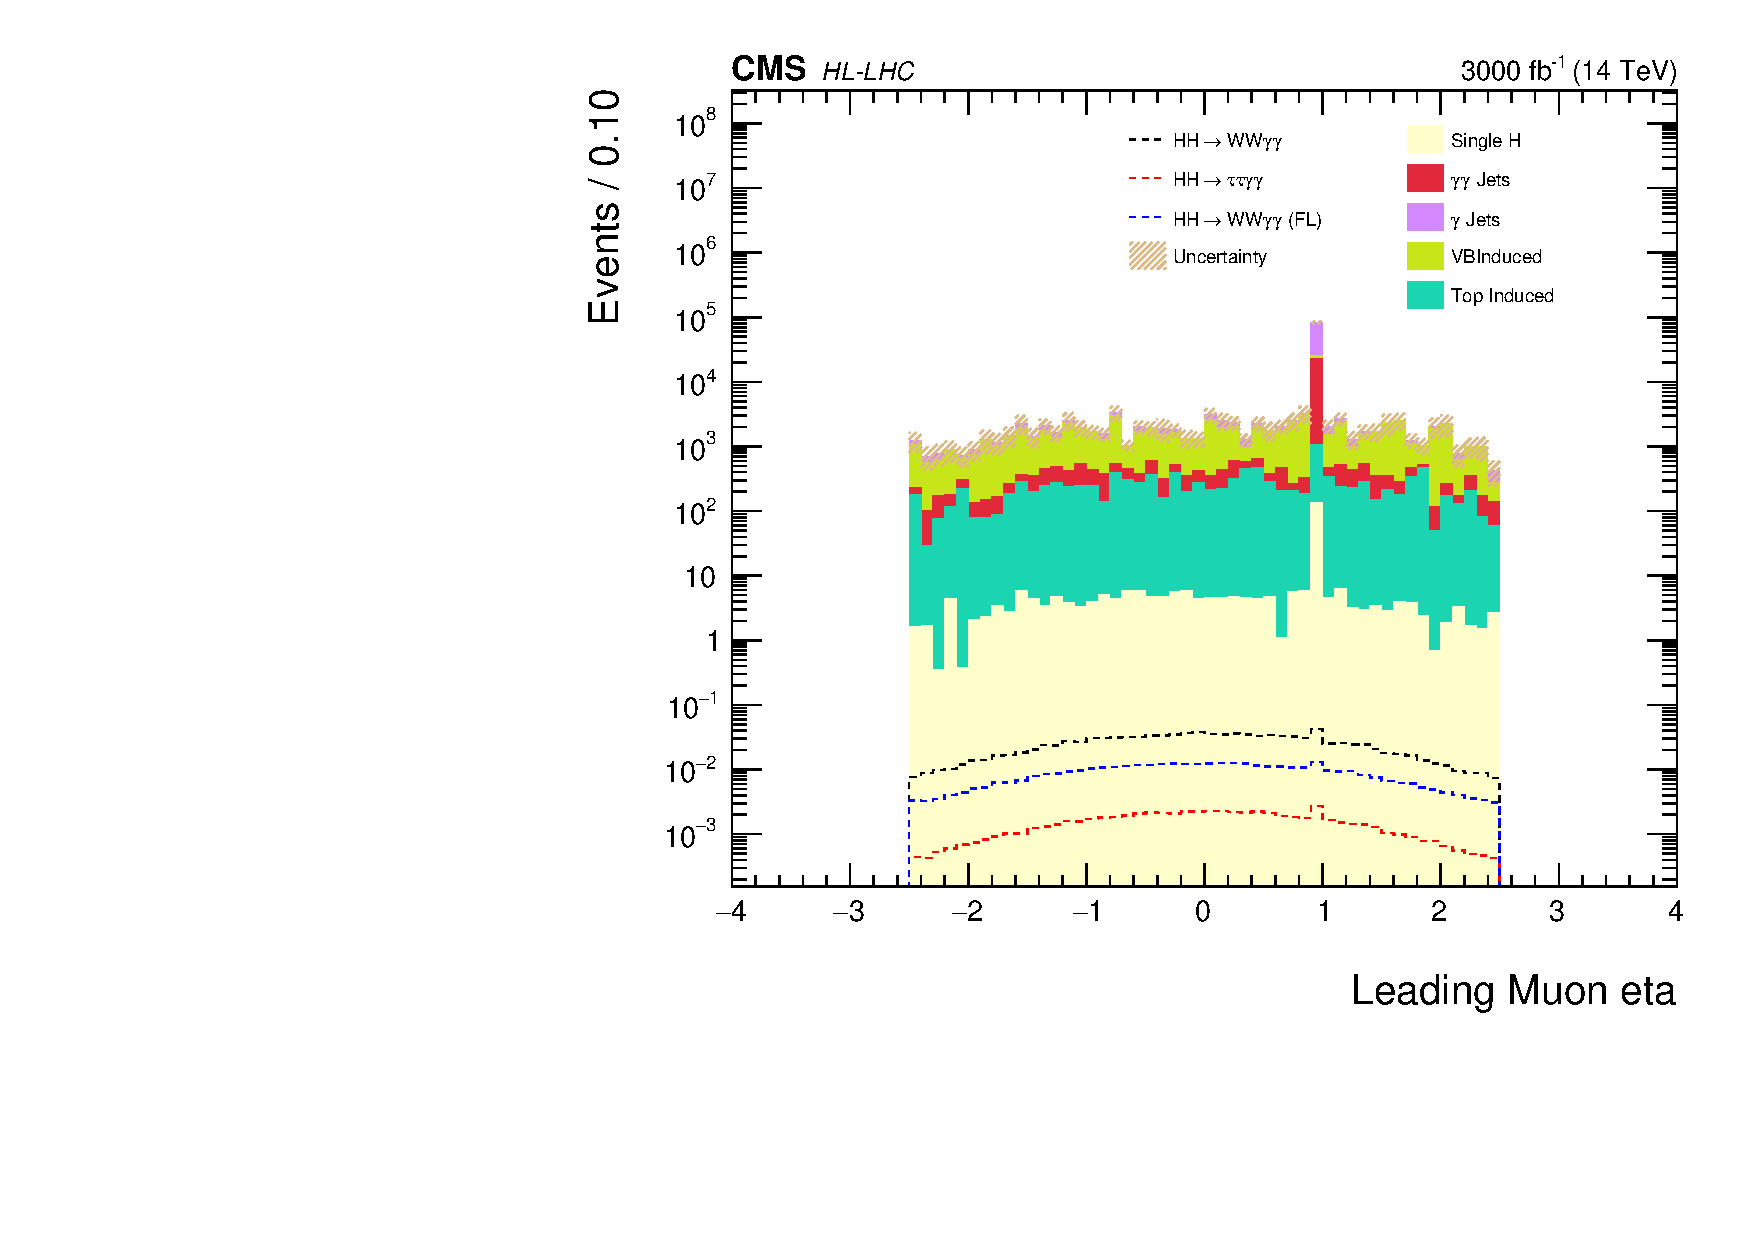
\includegraphics[width=\textwidth]{MuonEta_logy.pdf}
        \vspace{-0.5cm}
        \firstsubcaption{Leading Muon $\eta$}
    \end{subfigure}
    \vskip\baselineskip
    \begin{subfigure}[b]{0.475\textwidth}   
        \centering 
        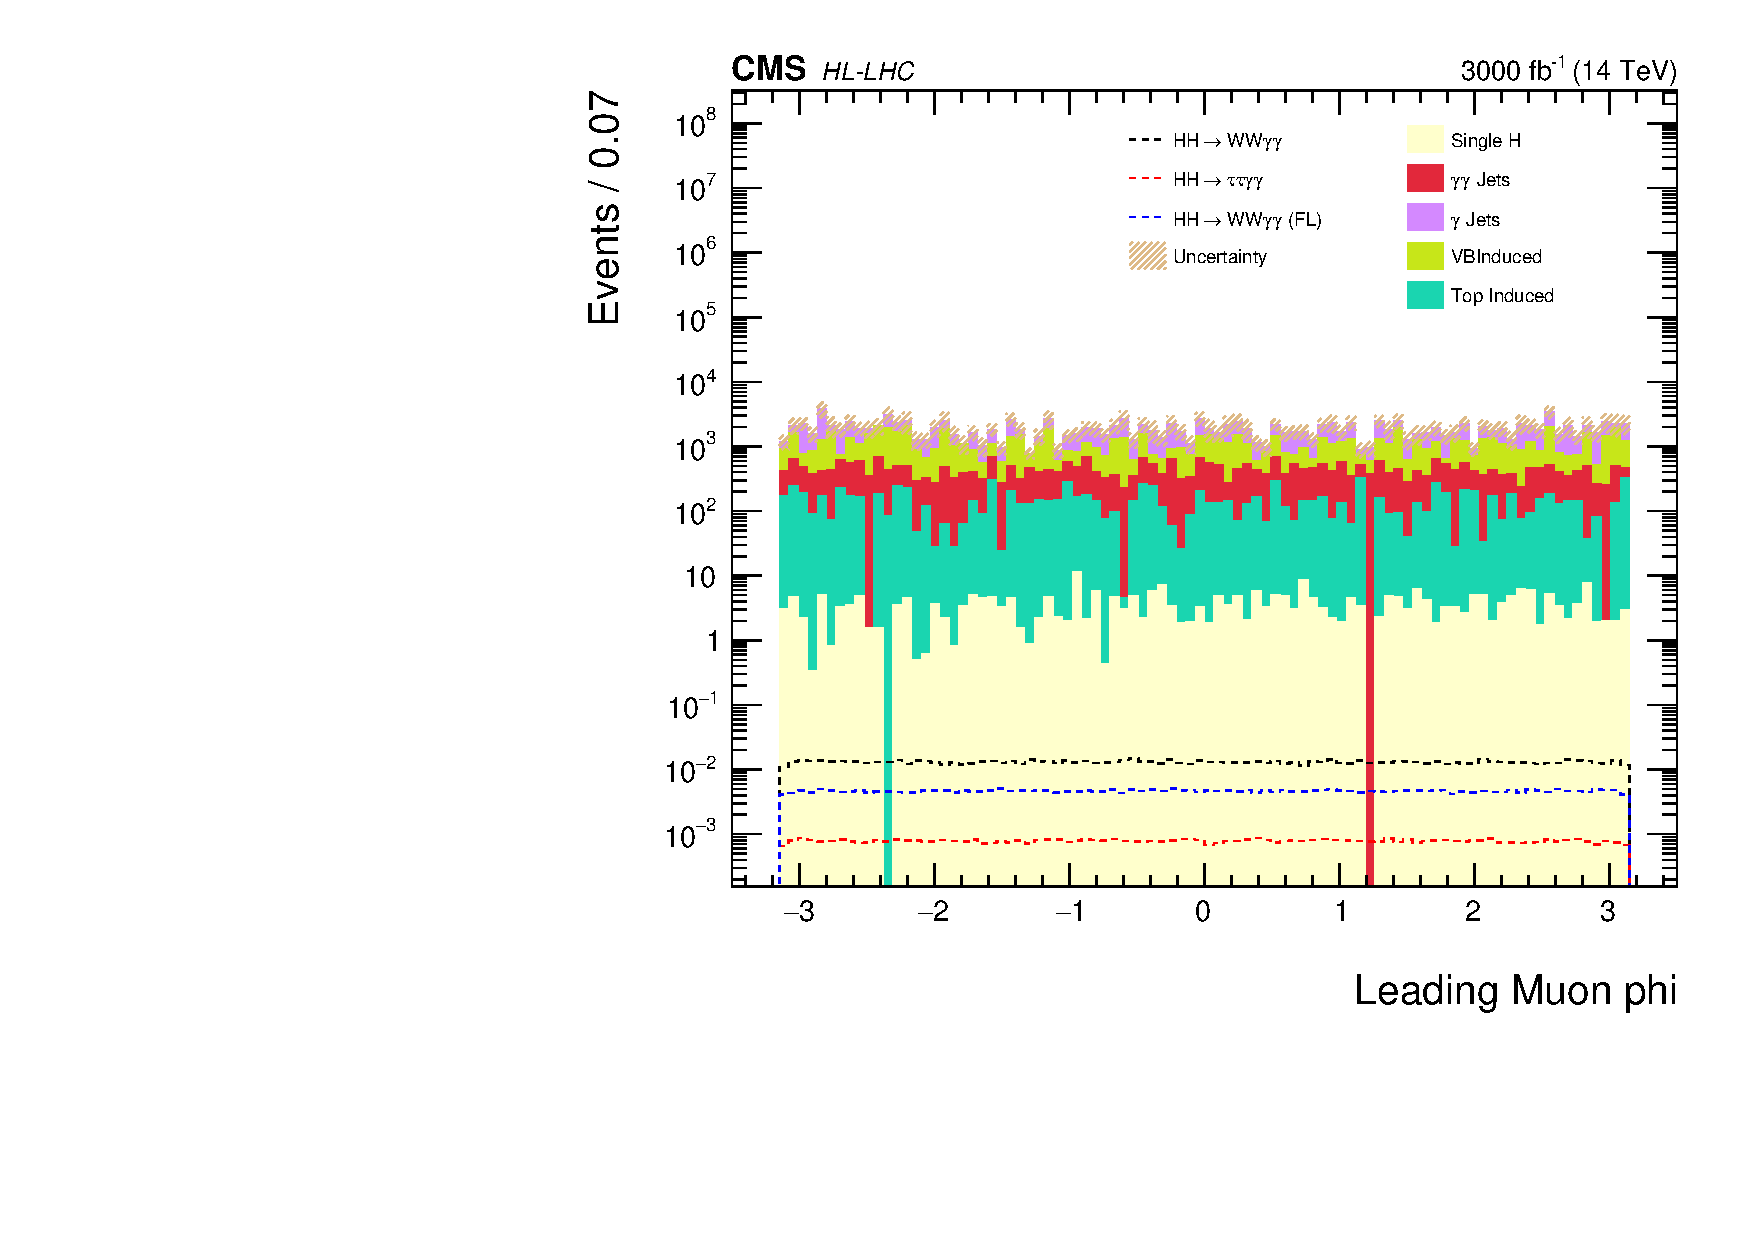
\includegraphics[width=\textwidth]{MuonPhi_logy.pdf}
        \vspace{-0.5cm}
        \firstsubcaption{Leading Muon $\phi$}
    \end{subfigure}
    \hfill
    \begin{subfigure}[b]{0.475\textwidth}   
        \centering 
        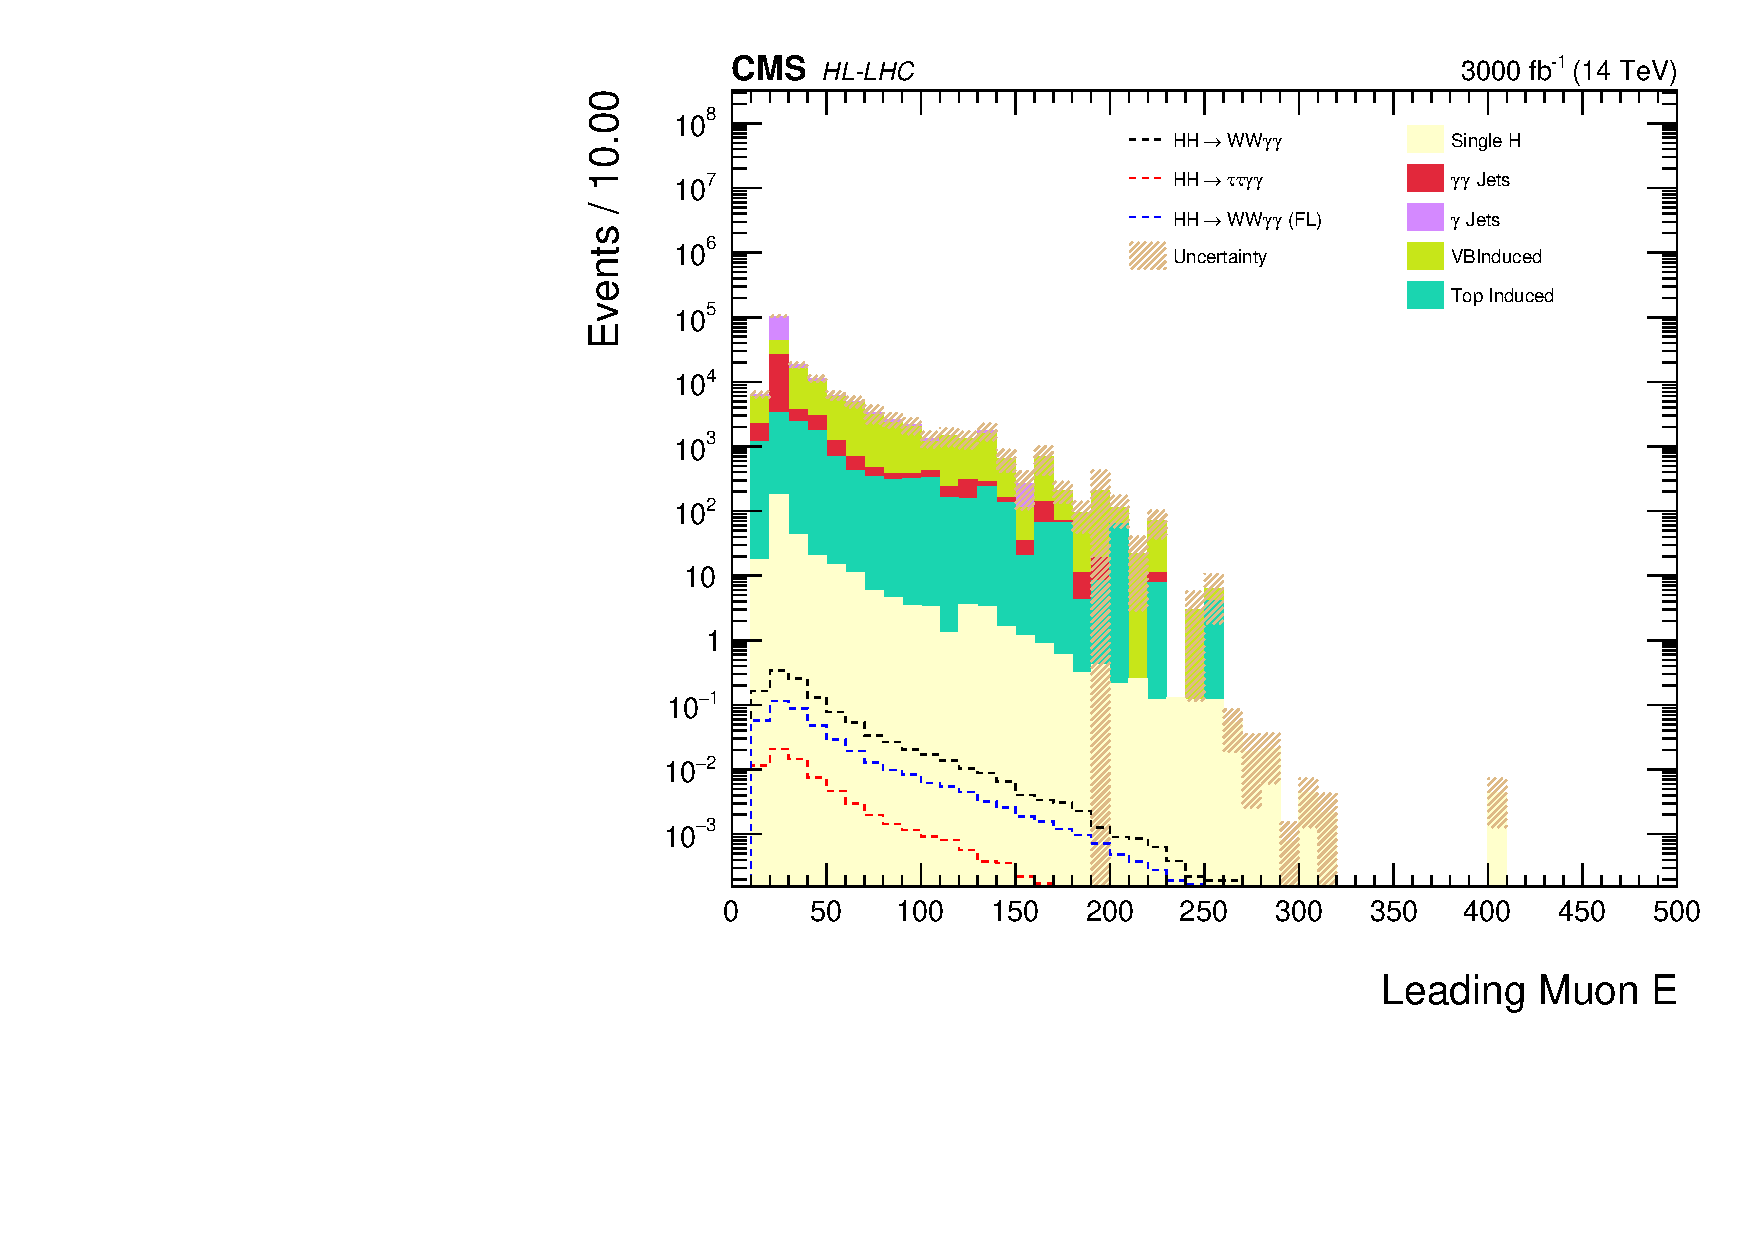
\includegraphics[width=\textwidth]{MuonE_logy.pdf}
        \vspace{-0.5cm}
        \firstsubcaption{Leading Muon energy}
    \end{subfigure}
    \vskip\baselineskip
    \begin{subfigure}[b]{0.475\textwidth}   
        \centering 
        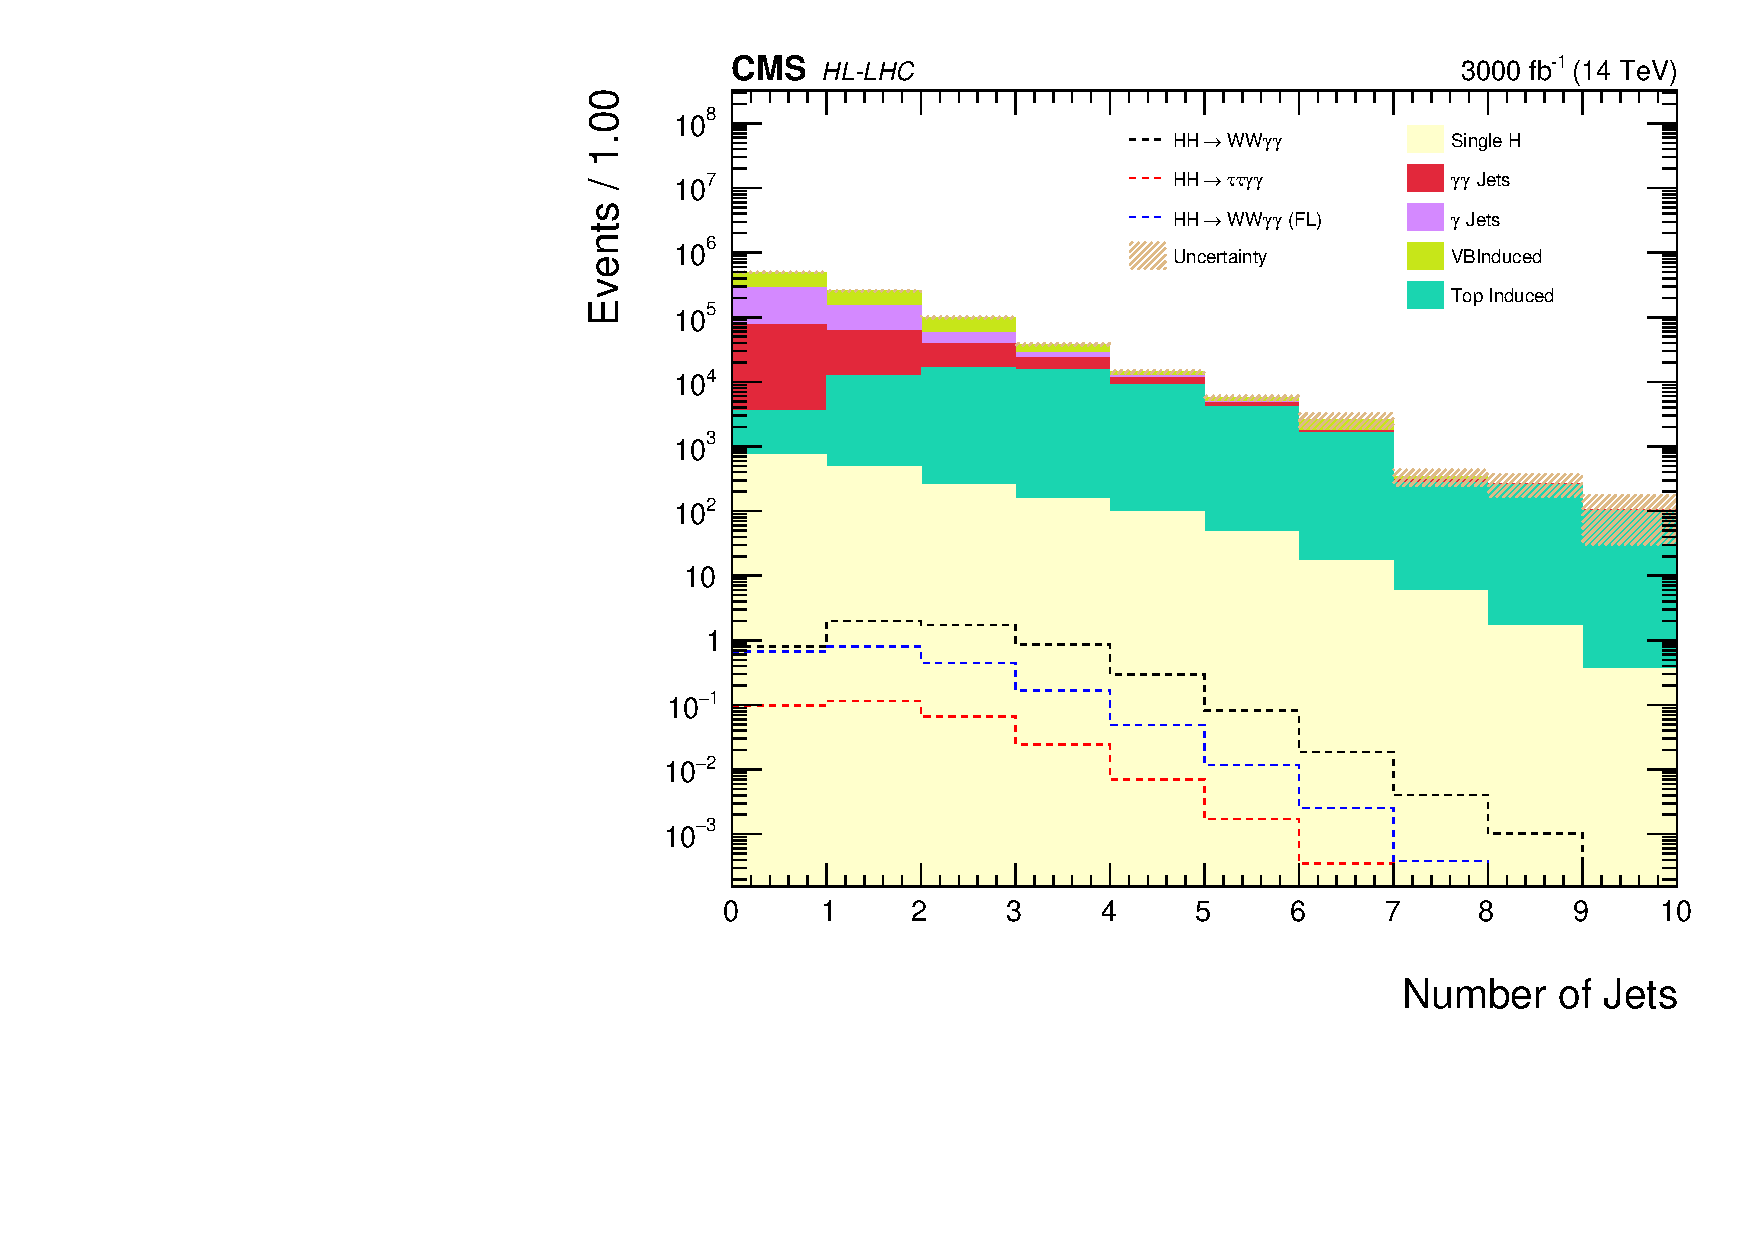
\includegraphics[width=\textwidth]{nJetsOneL_logy.pdf}
        \vspace{-0.5cm}
        \firstsubcaption{Jet multiplicity}
    \end{subfigure}
    \hfill
    \begin{subfigure}[b]{0.475\textwidth}   
        \centering 
        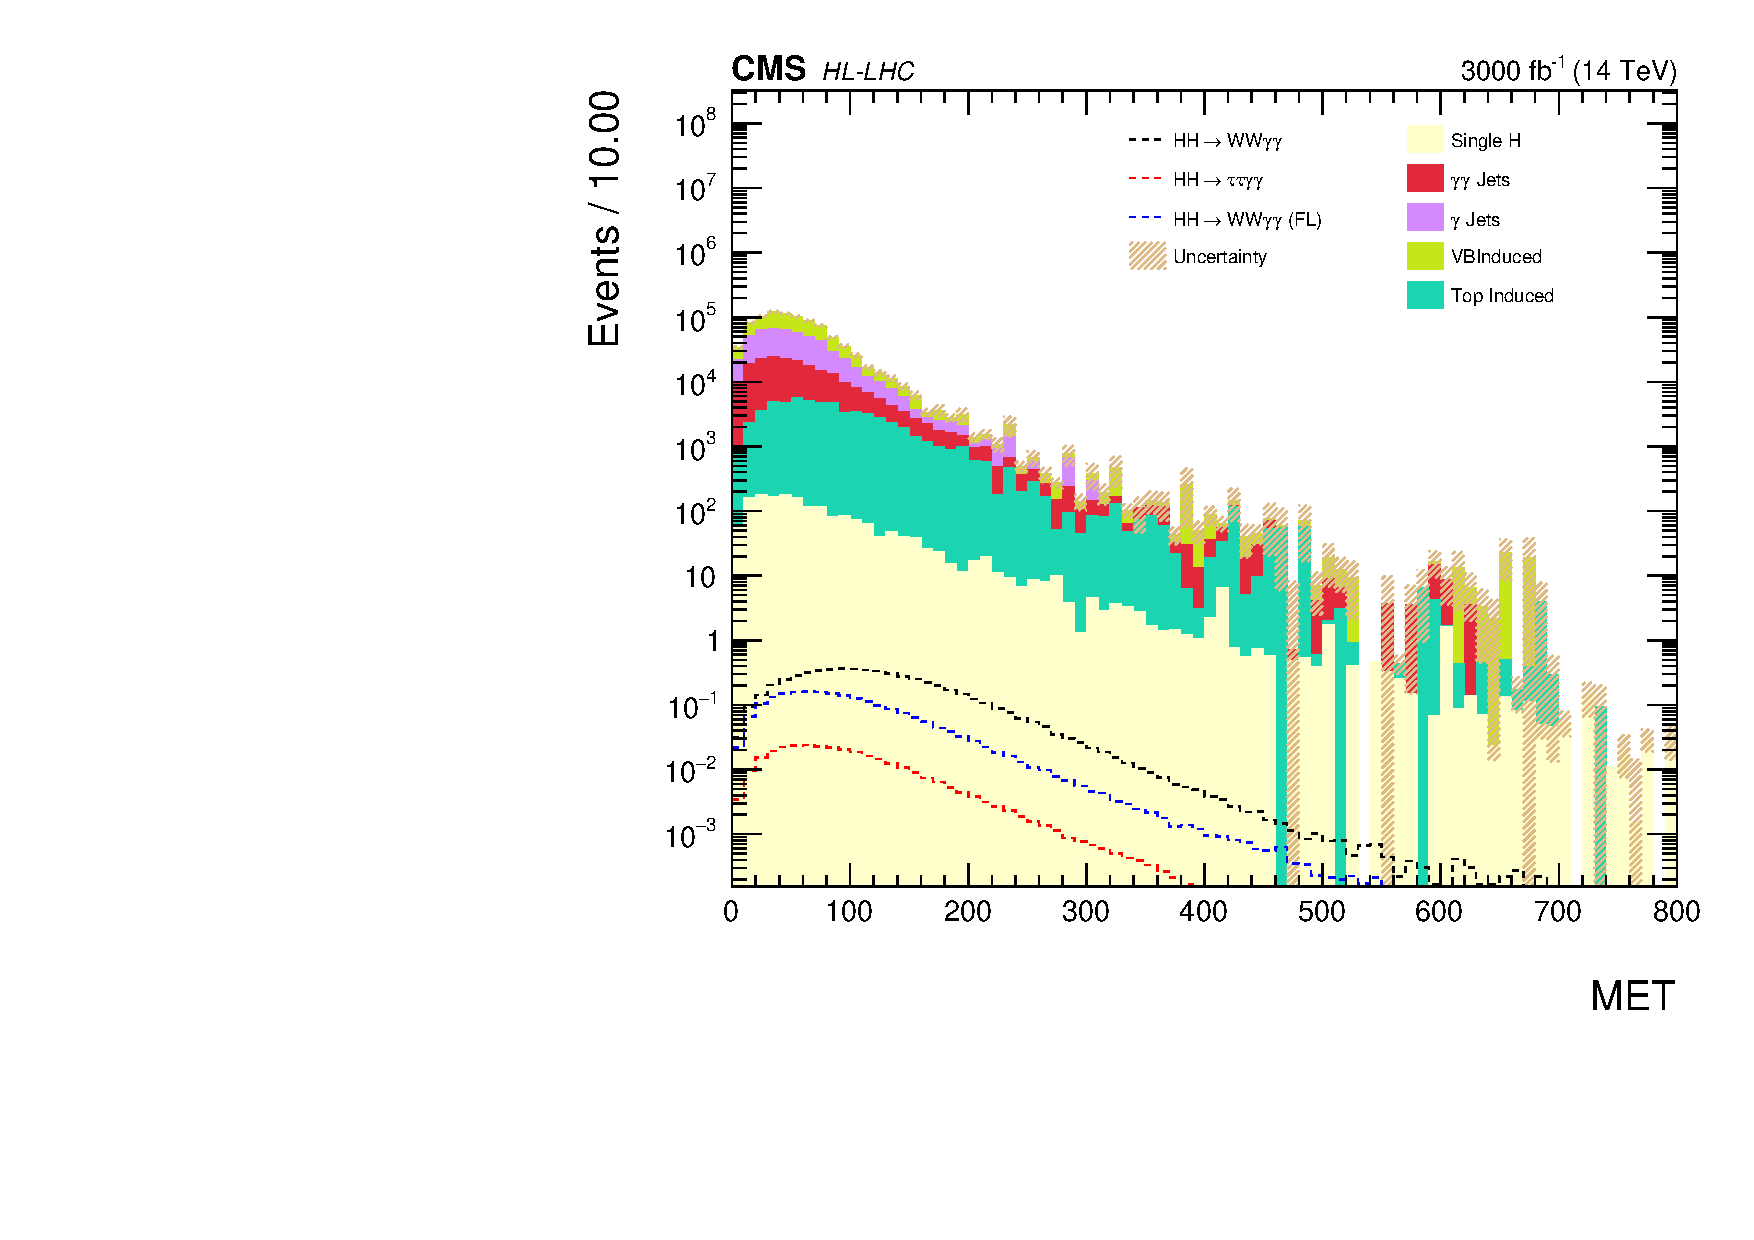
\includegraphics[width=\textwidth]{MET_logy.pdf}
        \vspace{-0.5cm}
        \firstsubcaption{$E_T^{miss}$}   
    \end{subfigure}
    \caption{\small DNN input distributions for the semi-leptonic final state (continued).}
\end{figure*}
\newpage

\begin{figure*}[h!]
    \centering
    \begin{subfigure}[b]{0.475\textwidth}
        \centering
        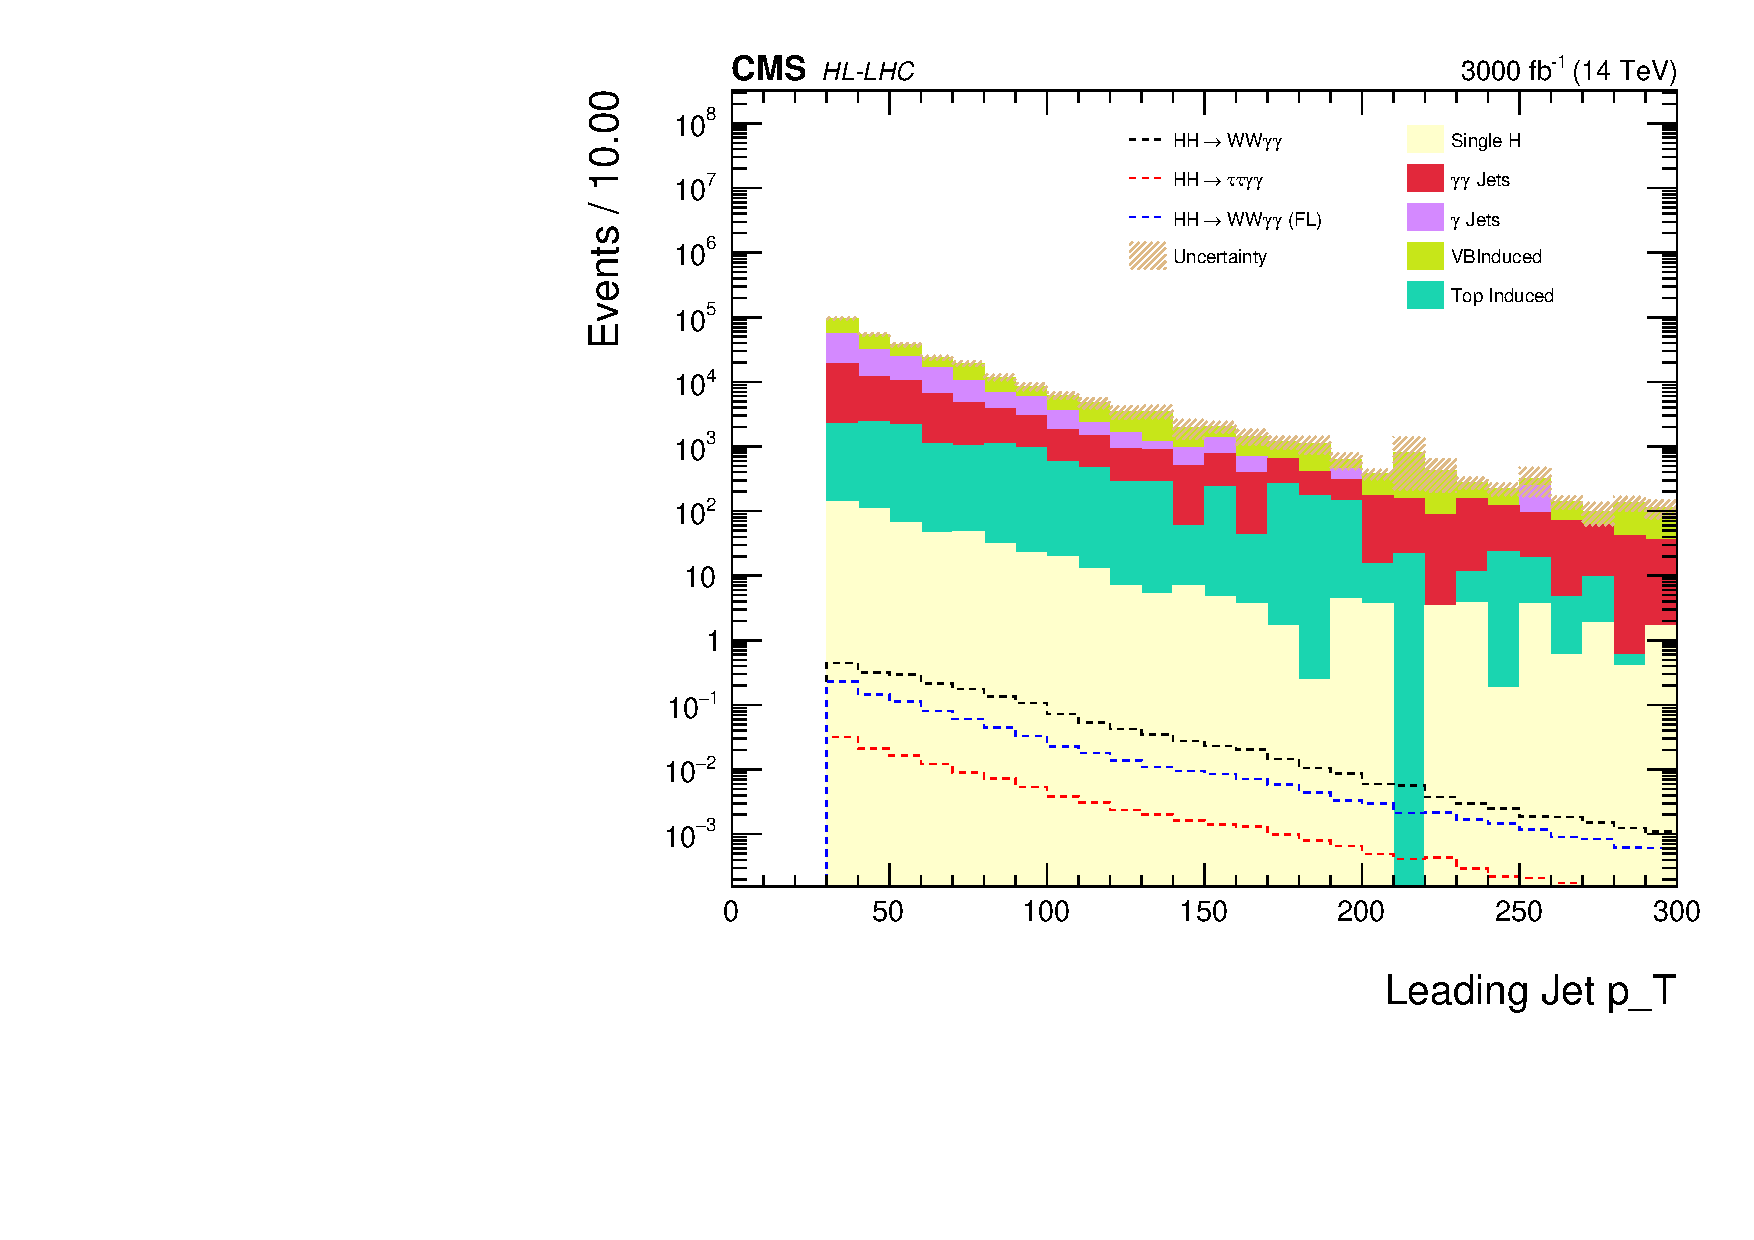
\includegraphics[width=\textwidth]{hasonel_hasOneJ_jetpt_logy.pdf}
        \vspace{-0.5cm}
        \firstsubcaption{Leading jet \pt}
    \end{subfigure}
    \hfill
    \begin{subfigure}[b]{0.475\textwidth}  
        \centering 
        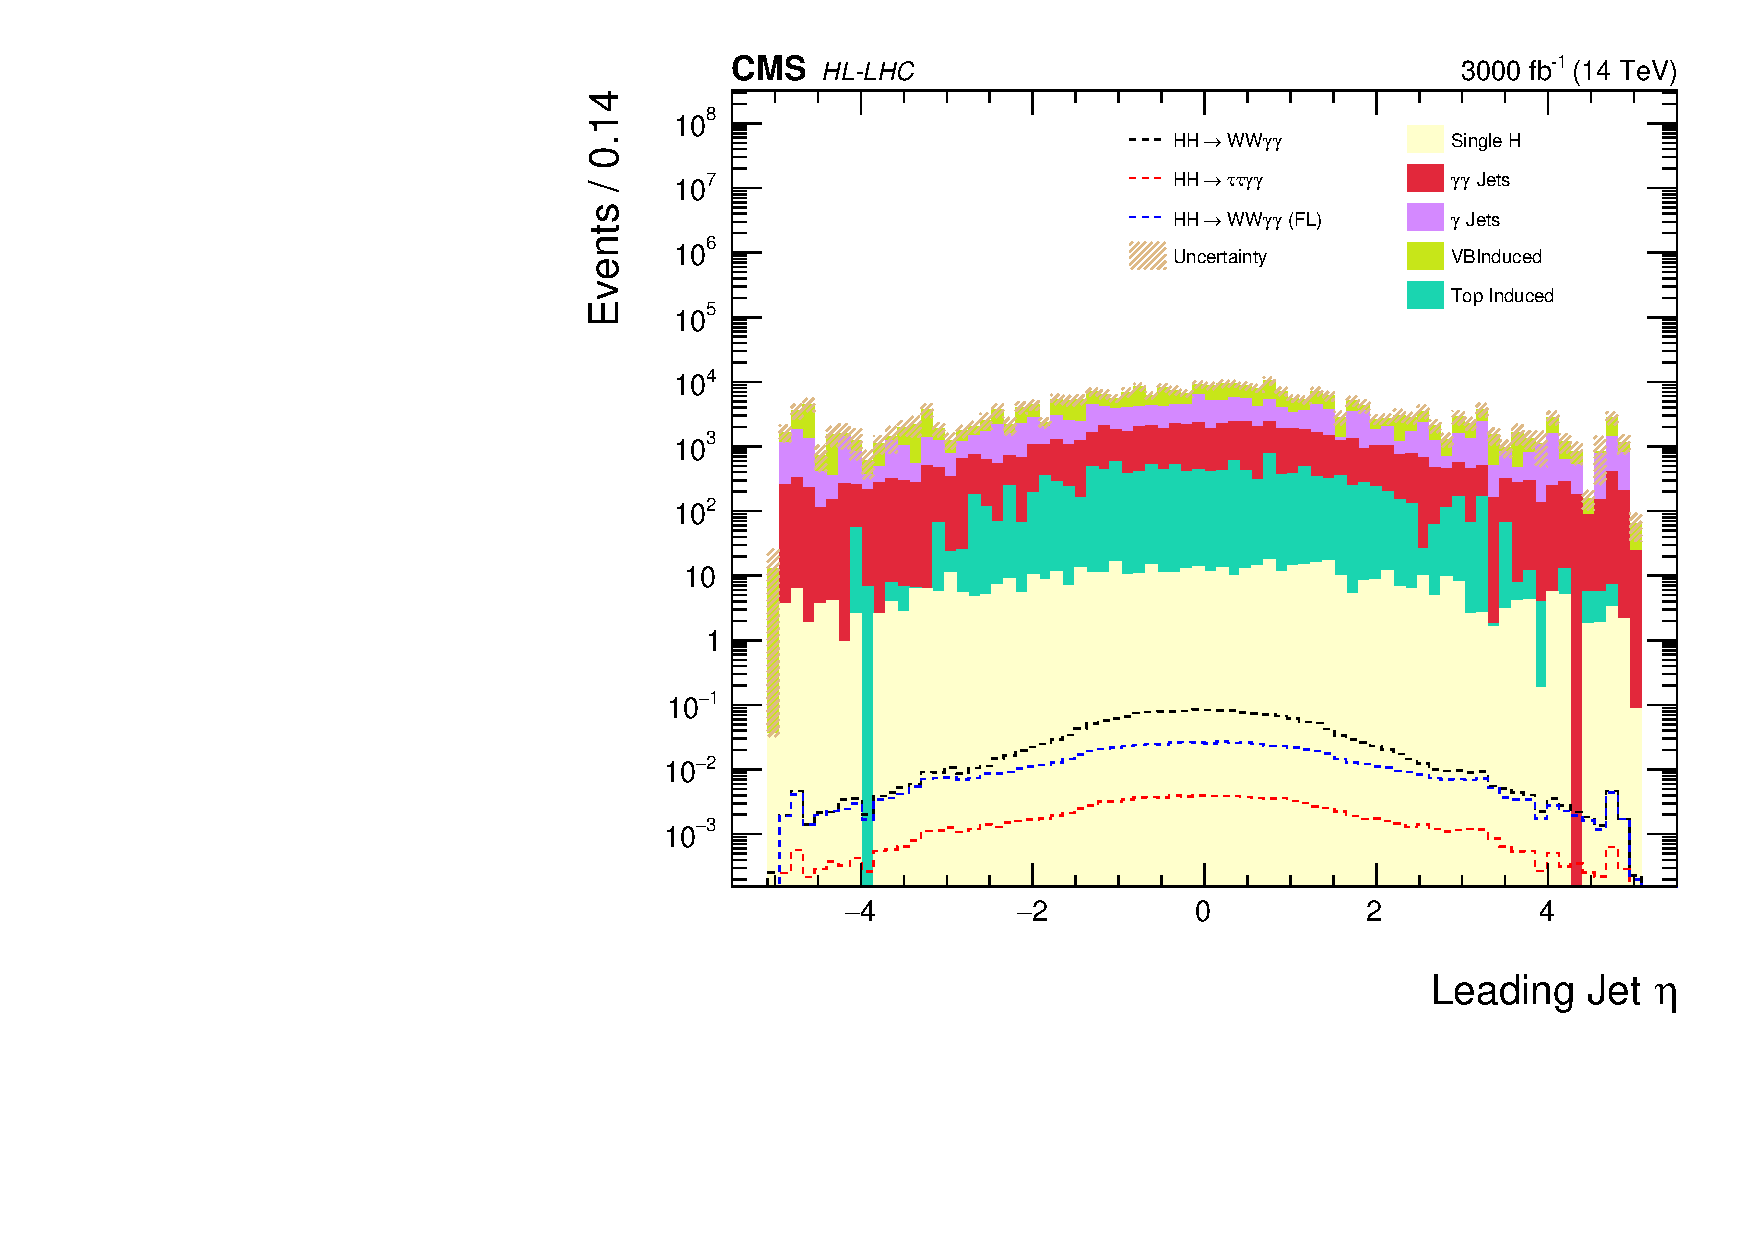
\includegraphics[width=\textwidth]{hasonel_hasOneJ_jeteta_logy.pdf}
        \vspace{-0.5cm}
        \firstsubcaption{Leading jet $\eta$}
    \end{subfigure}
    \vskip\baselineskip
    \begin{subfigure}[b]{0.475\textwidth}   
        \centering 
        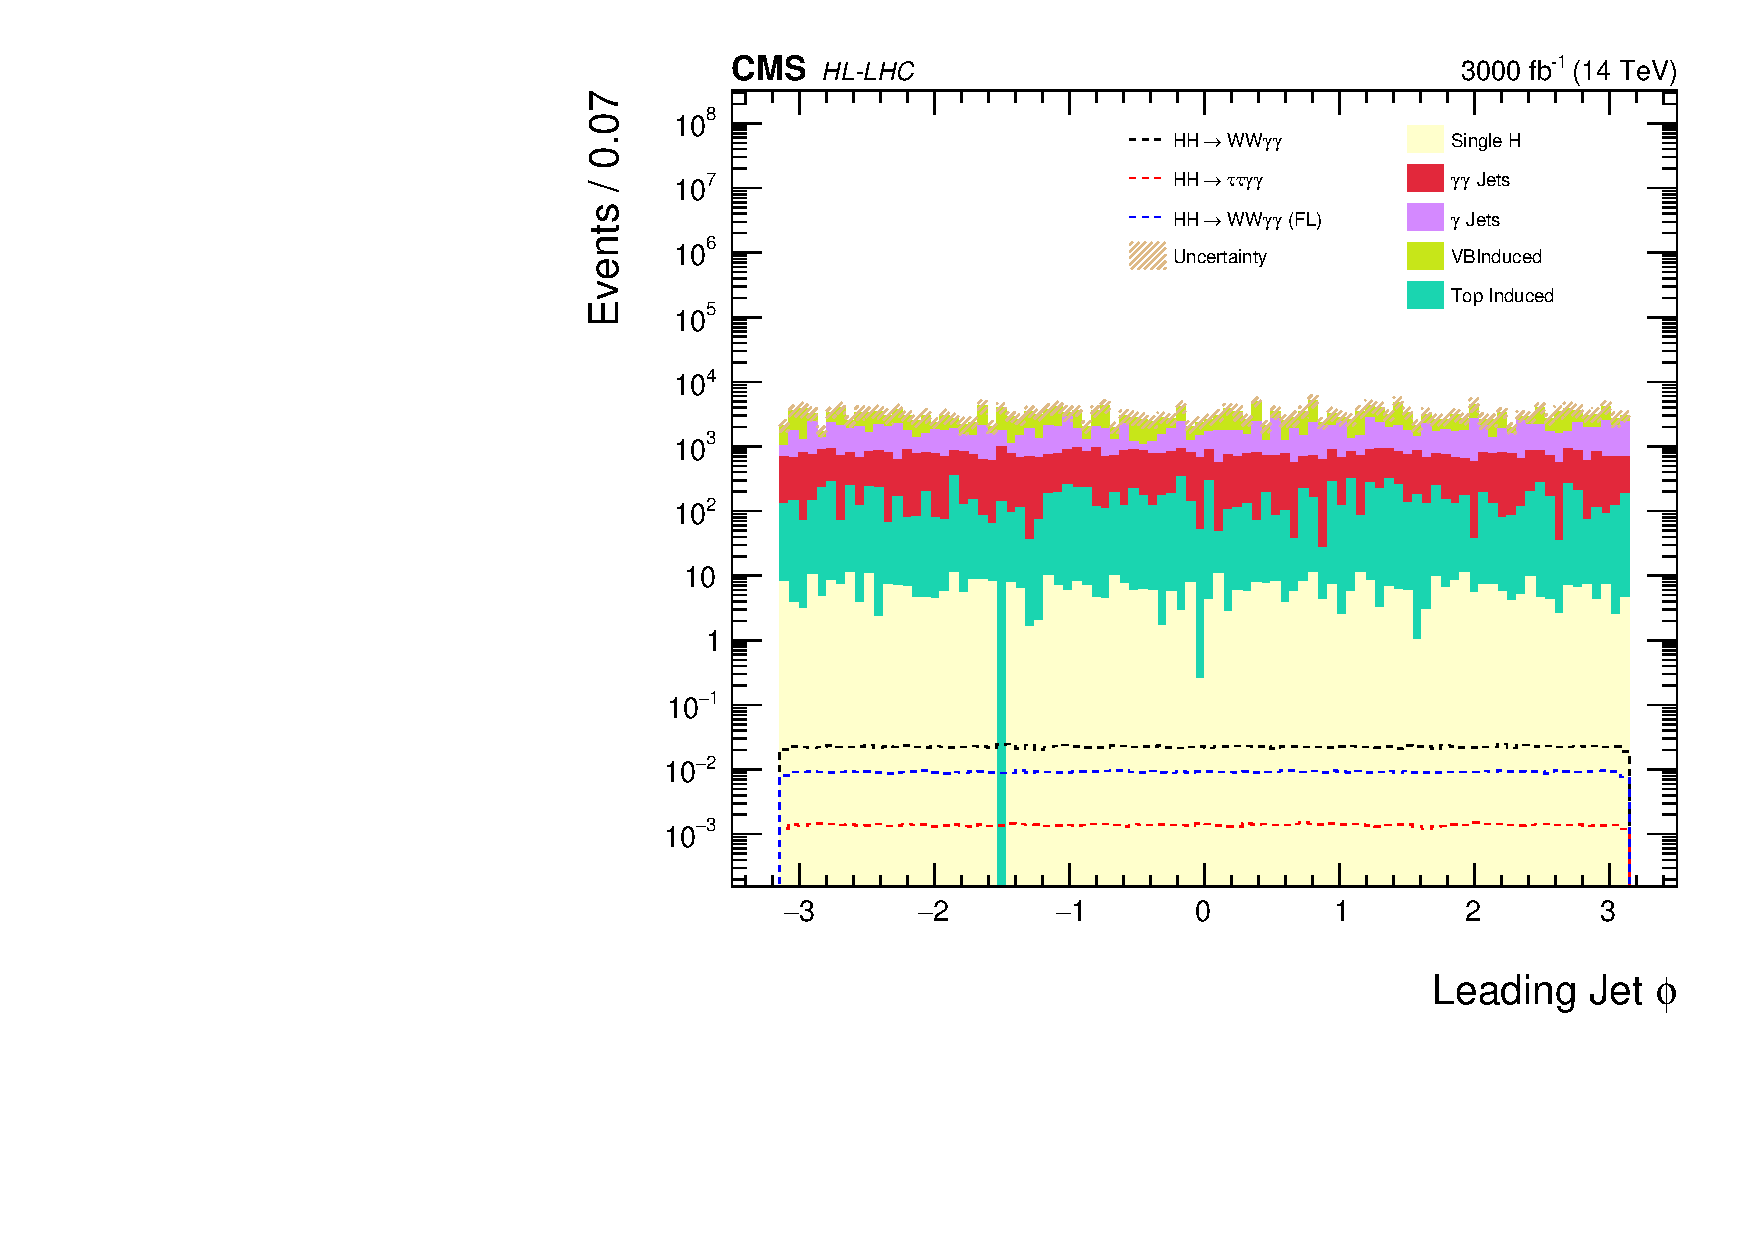
\includegraphics[width=\textwidth]{hasonel_hasOneJ_jetphi_logy.pdf}
        \vspace{-0.5cm}
        \firstsubcaption{Leading jet $\phi$}
    \end{subfigure}
    \hfill
    \begin{subfigure}[b]{0.475\textwidth}   
        \centering 
        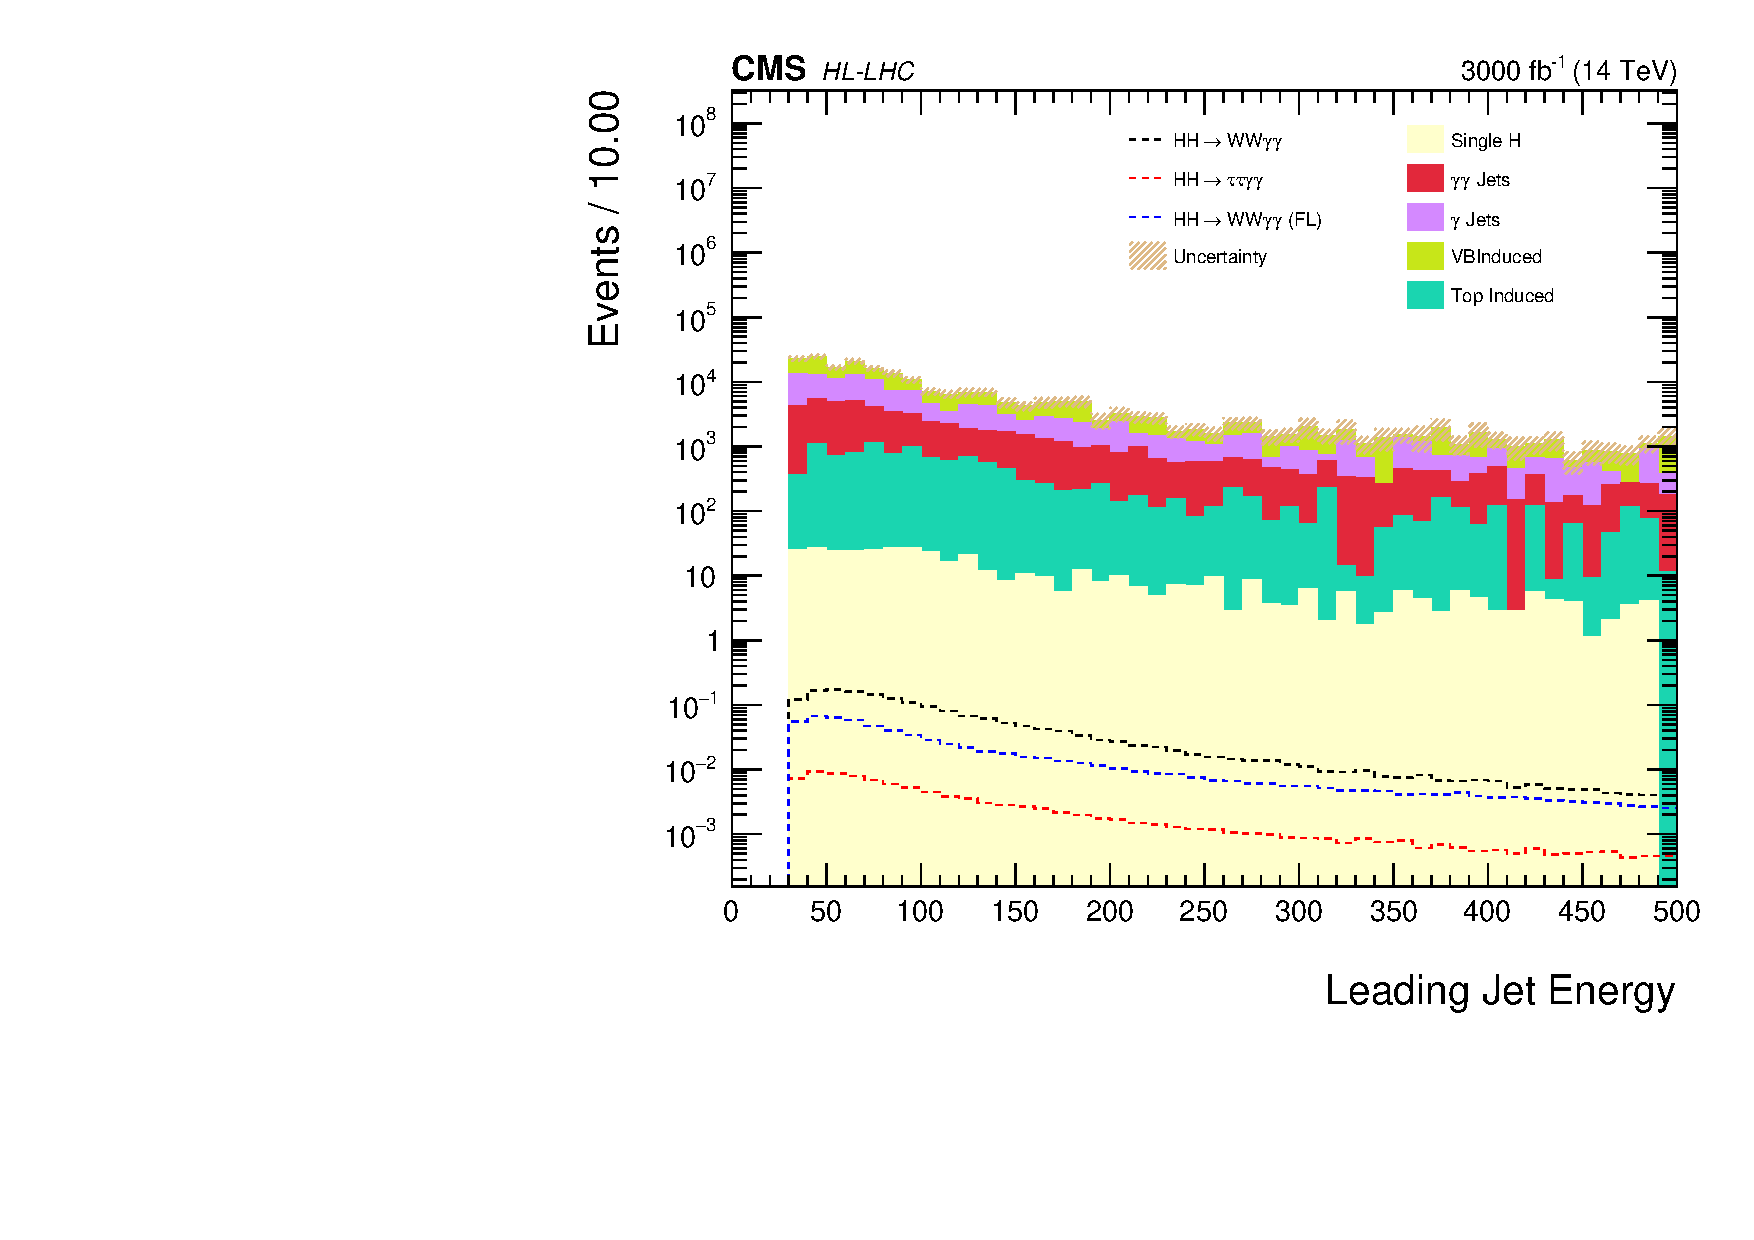
\includegraphics[width=\textwidth]{hasonel_hasOneJ_jetE_logy.pdf}
        \vspace{-0.5cm}
        \firstsubcaption{Leading jet energy}
    \end{subfigure}
    \vskip\baselineskip
    \begin{subfigure}[b]{0.475\textwidth}   
        \centering 
        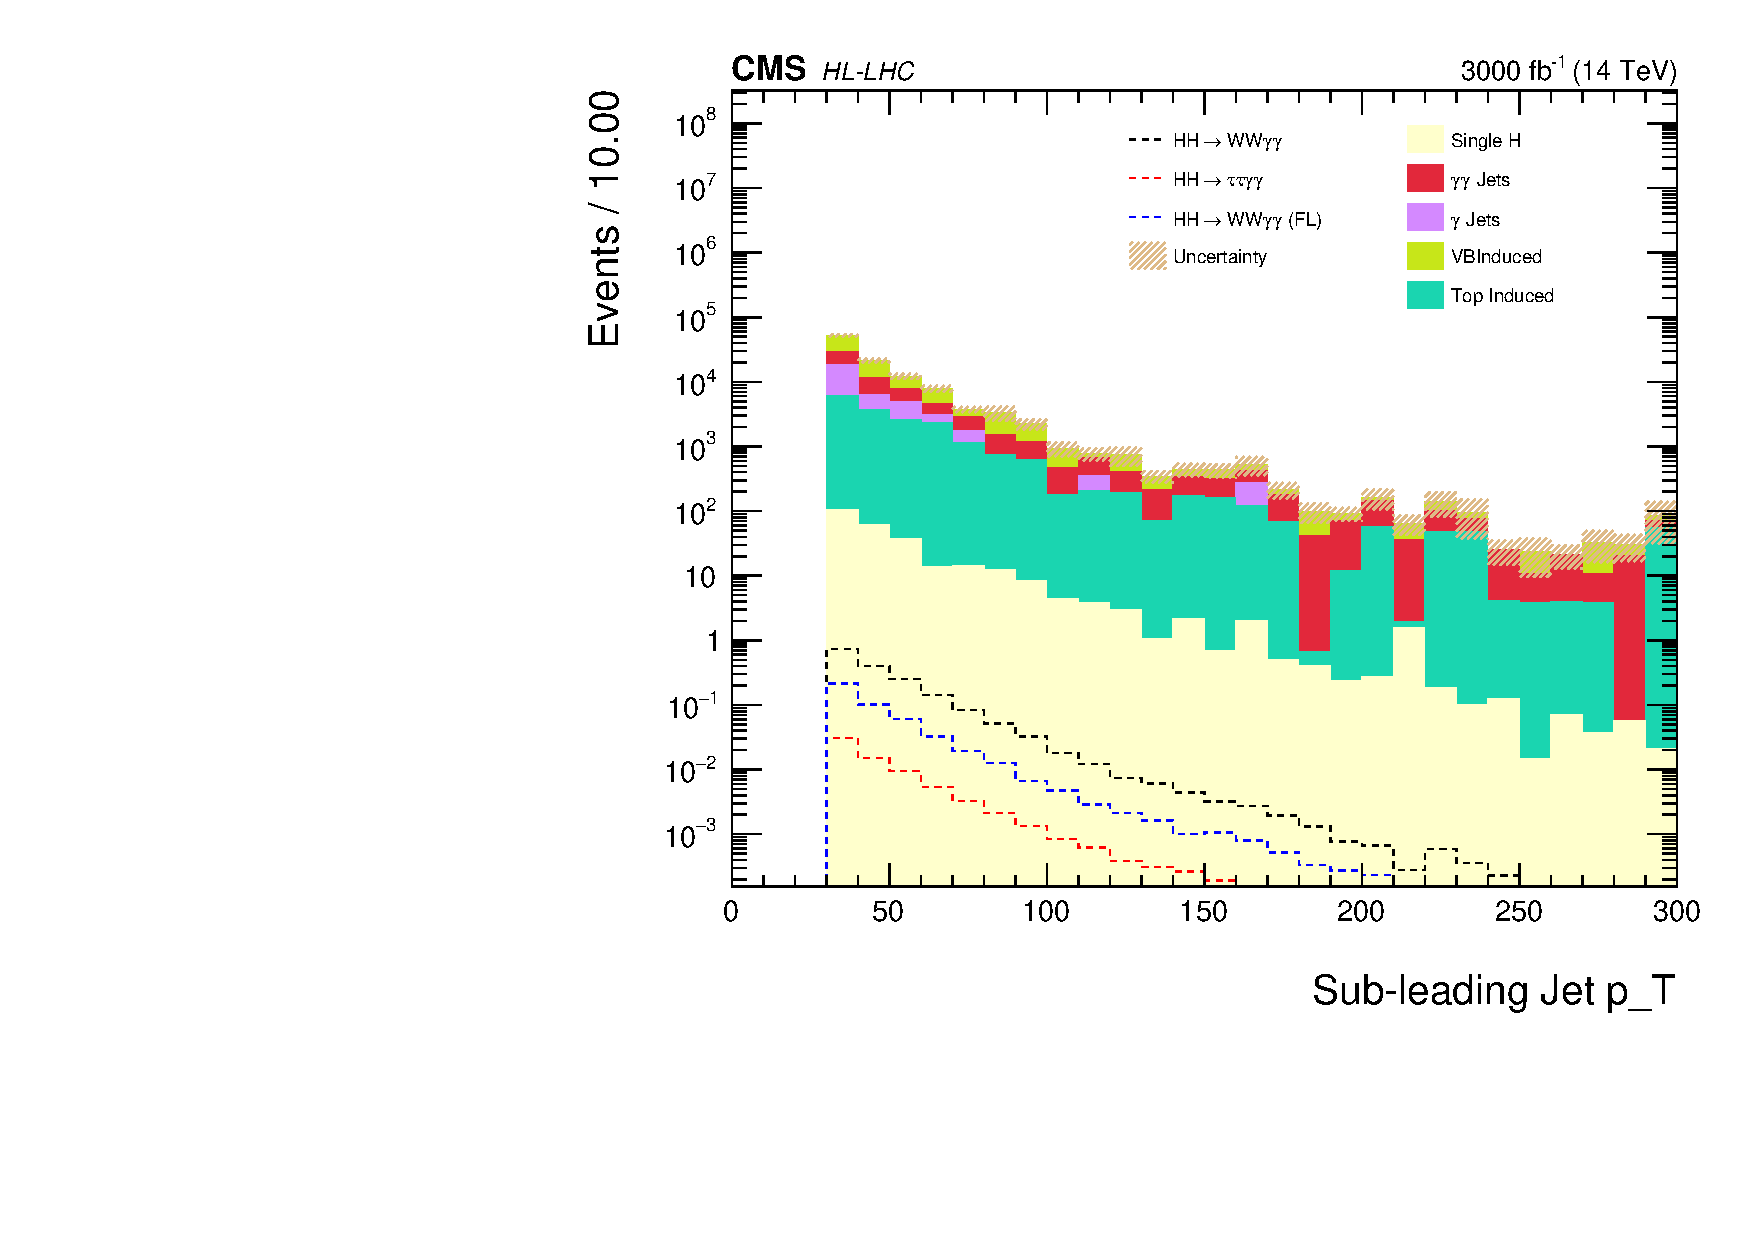
\includegraphics[width=\textwidth]{hasonel_hasTwoJ_jetpt_logy.pdf}
        \vspace{-0.5cm}
        \firstsubcaption{Sub-leading jet \pt}
    \end{subfigure}
    \hfill
    \begin{subfigure}[b]{0.475\textwidth}   
        \centering 
        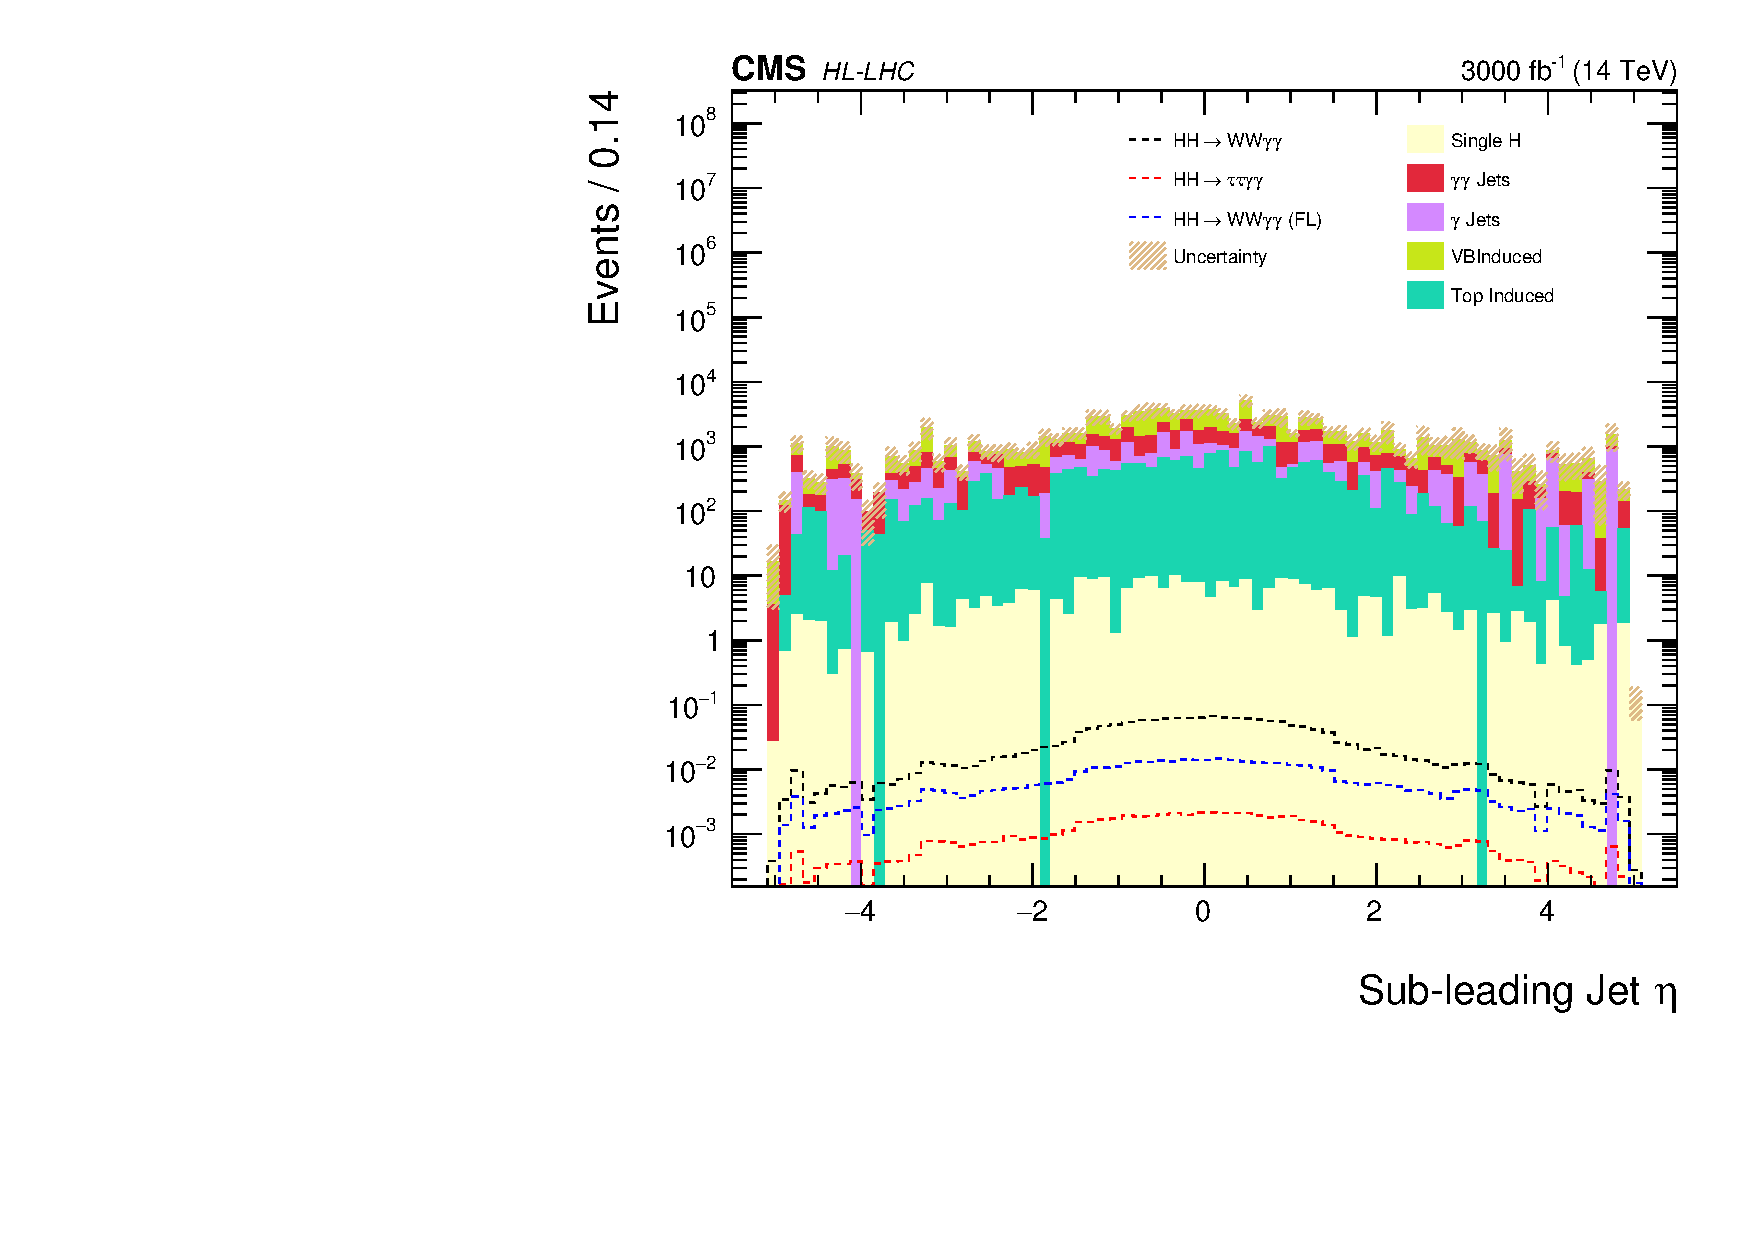
\includegraphics[width=\textwidth]{hasonel_hasTwoJ_jeteta_logy.pdf}
        \vspace{-0.5cm}
        \firstsubcaption{Sub-leading jet $\eta$}   
    \end{subfigure}
    \caption{\small DNN input distributions for the semi-leptonic final state (continued).}
\end{figure*}
\newpage

\begin{figure*}[h!]
    \centering
    \begin{subfigure}[b]{0.475\textwidth}
        \centering
        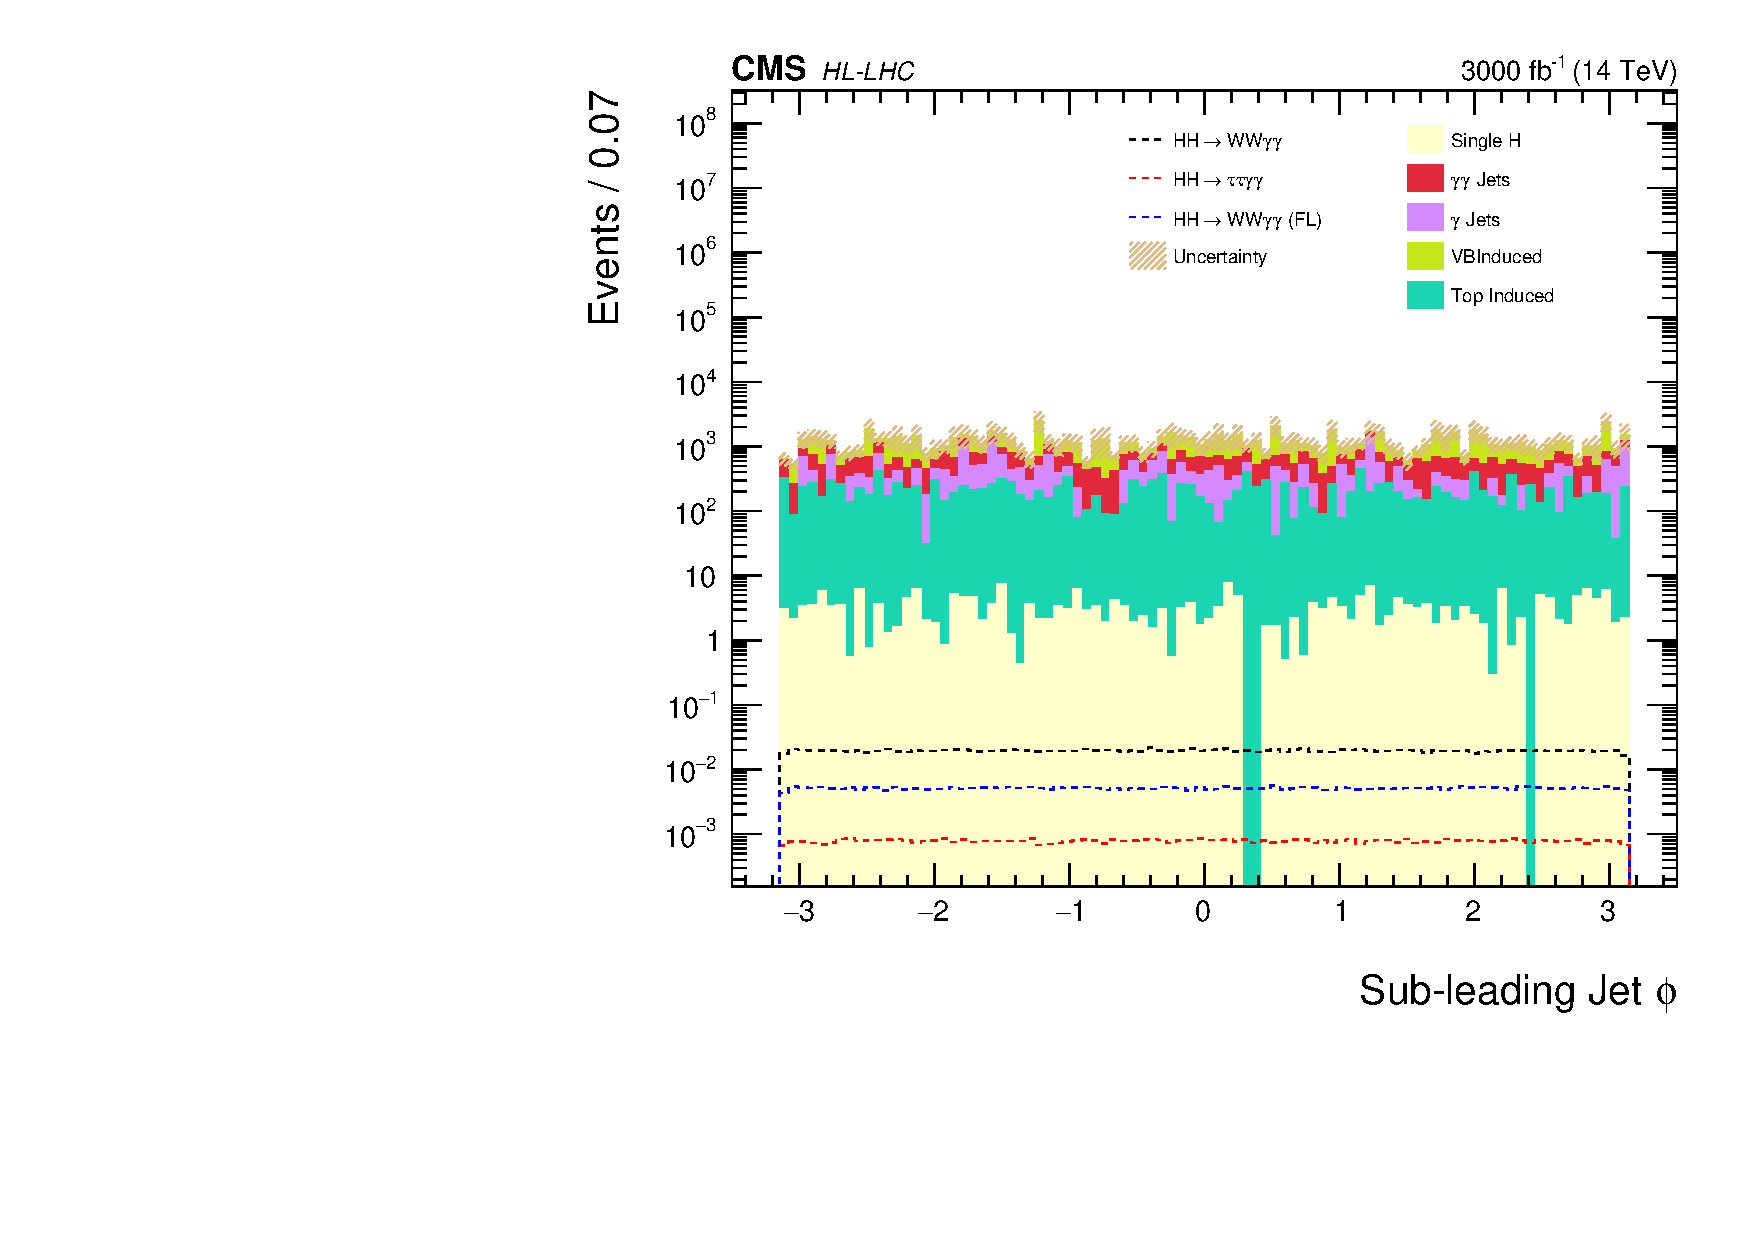
\includegraphics[width=\textwidth]{hasonel_hasTwoJ_jetphi_logy.pdf}
        \vspace{-0.5cm}
        \firstsubcaption{Sub-leading jet $\phi$}
    \end{subfigure}
    \hfill
    \begin{subfigure}[b]{0.475\textwidth}  
        \centering 
        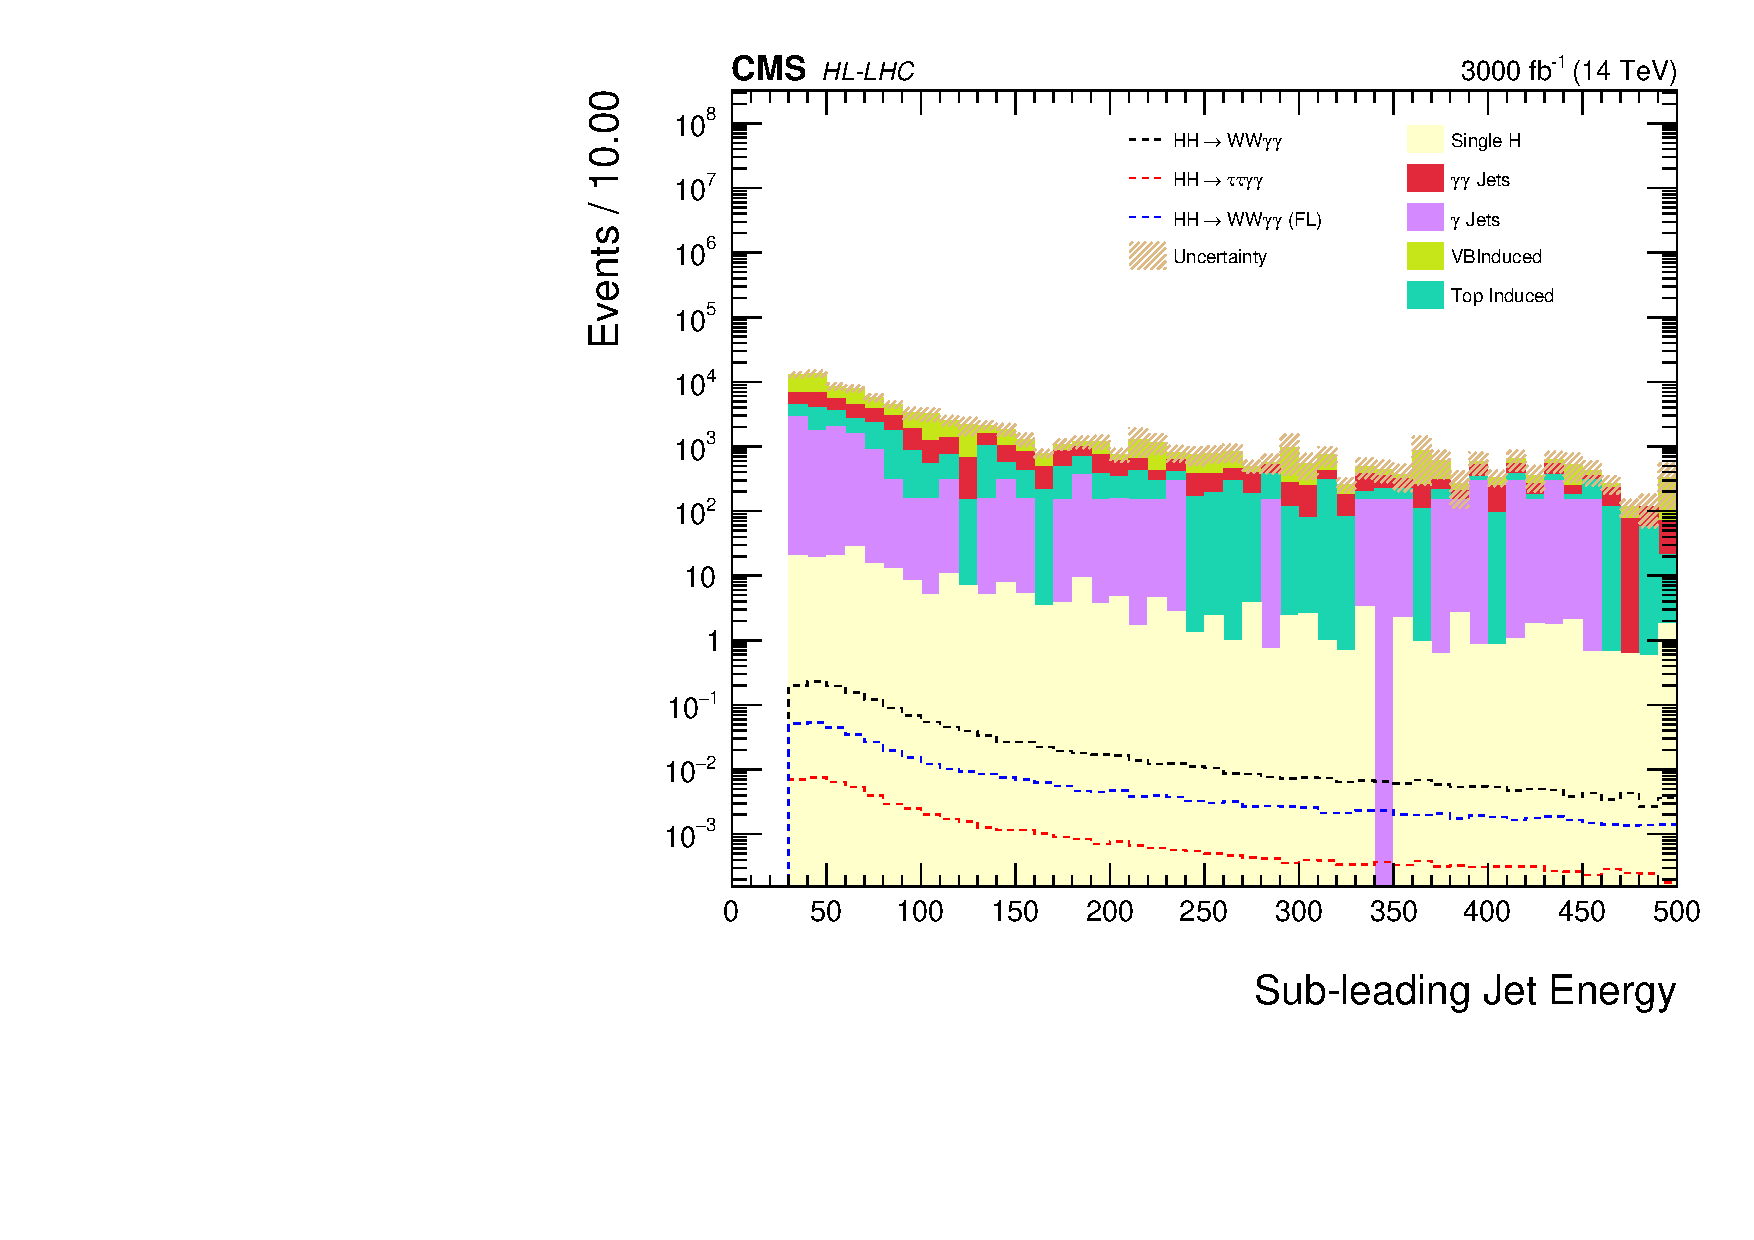
\includegraphics[width=\textwidth]{hasonel_hasTwoJ_jetE_logy.pdf}
        \vspace{-0.5cm}
        \firstsubcaption{Sub-leading jet energy}
    \end{subfigure}
    \vskip\baselineskip
    \begin{subfigure}[b]{0.475\textwidth}   
        \centering 
        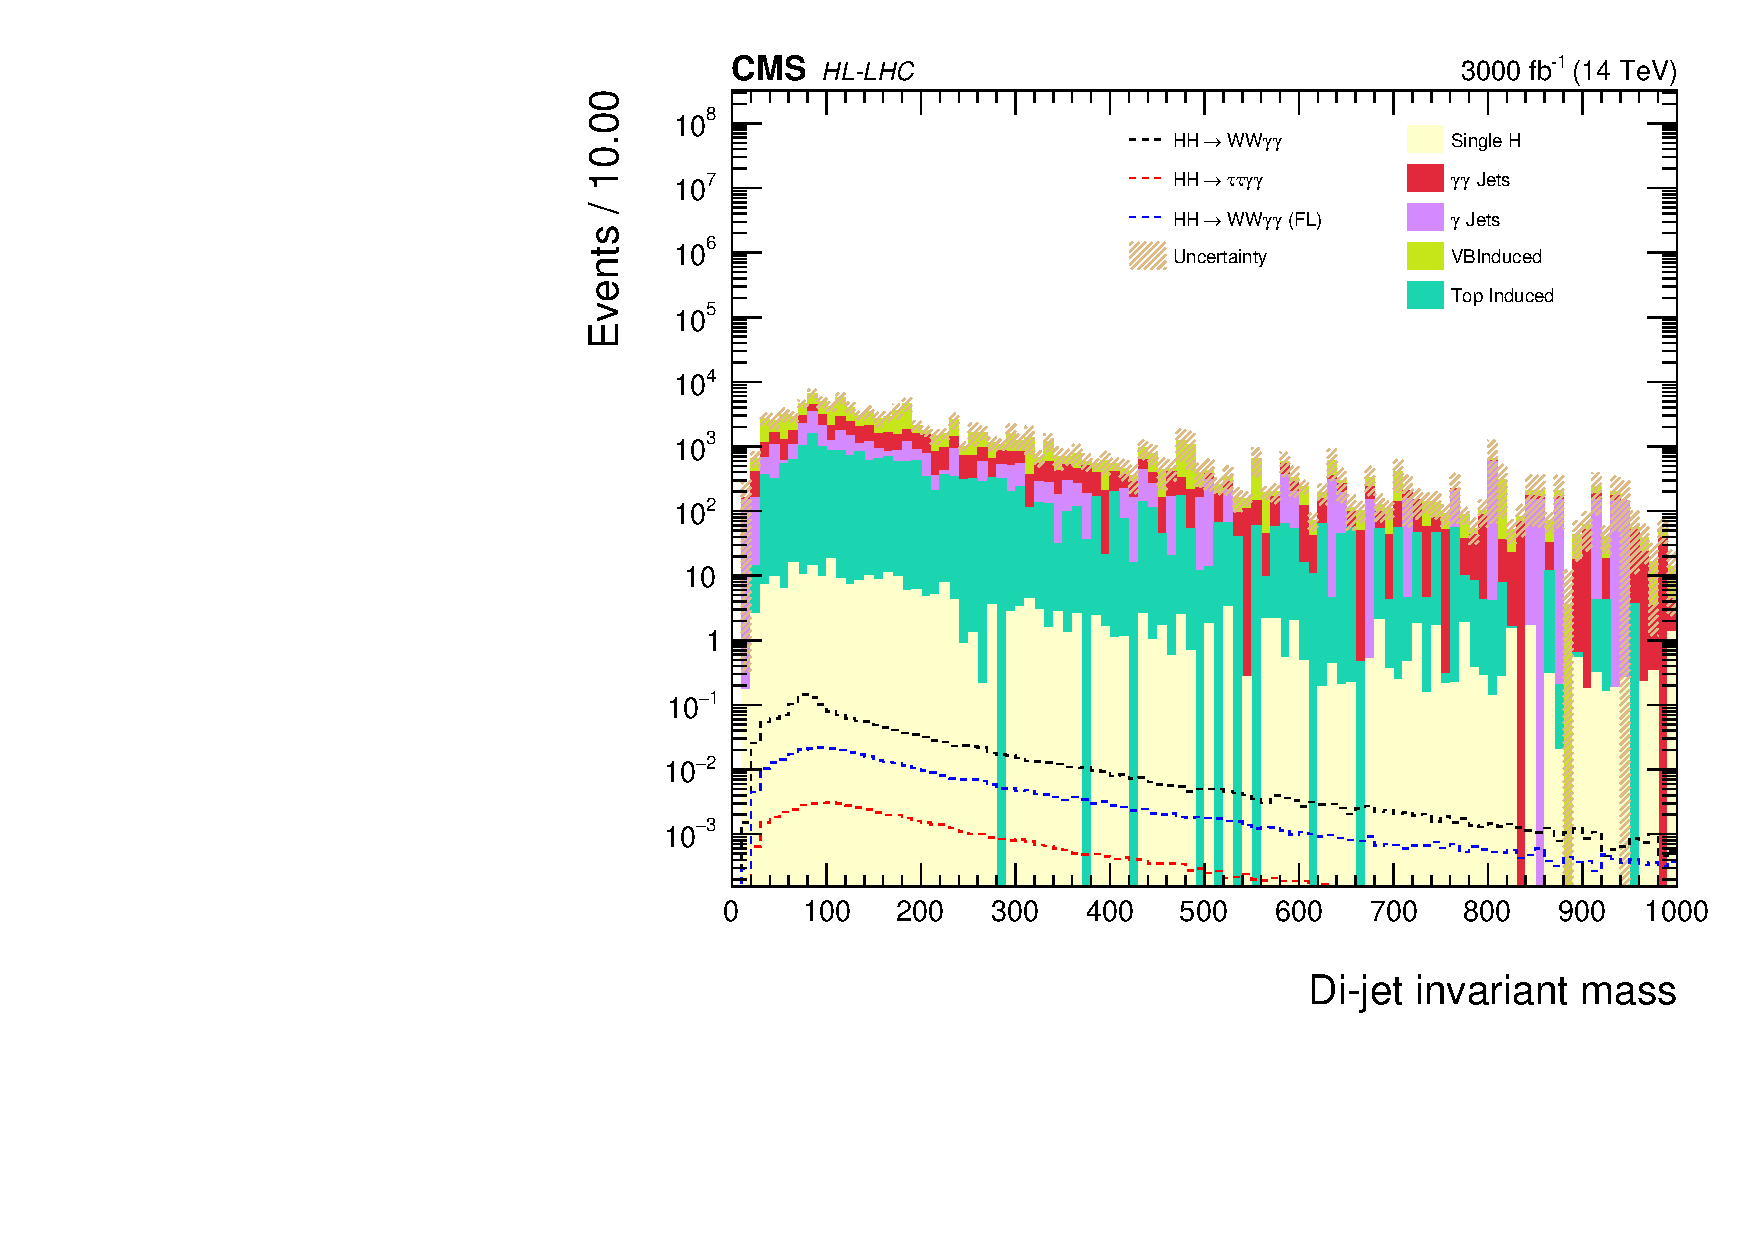
\includegraphics[width=\textwidth]{hasonel_hastwoJ_mjj_logy.pdf}
        \vspace{-0.5cm}
        \firstsubcaption{$m_{j_0,j_1}$}
    \end{subfigure}
    \hfill
    \begin{subfigure}[b]{0.475\textwidth}   
        \centering 
        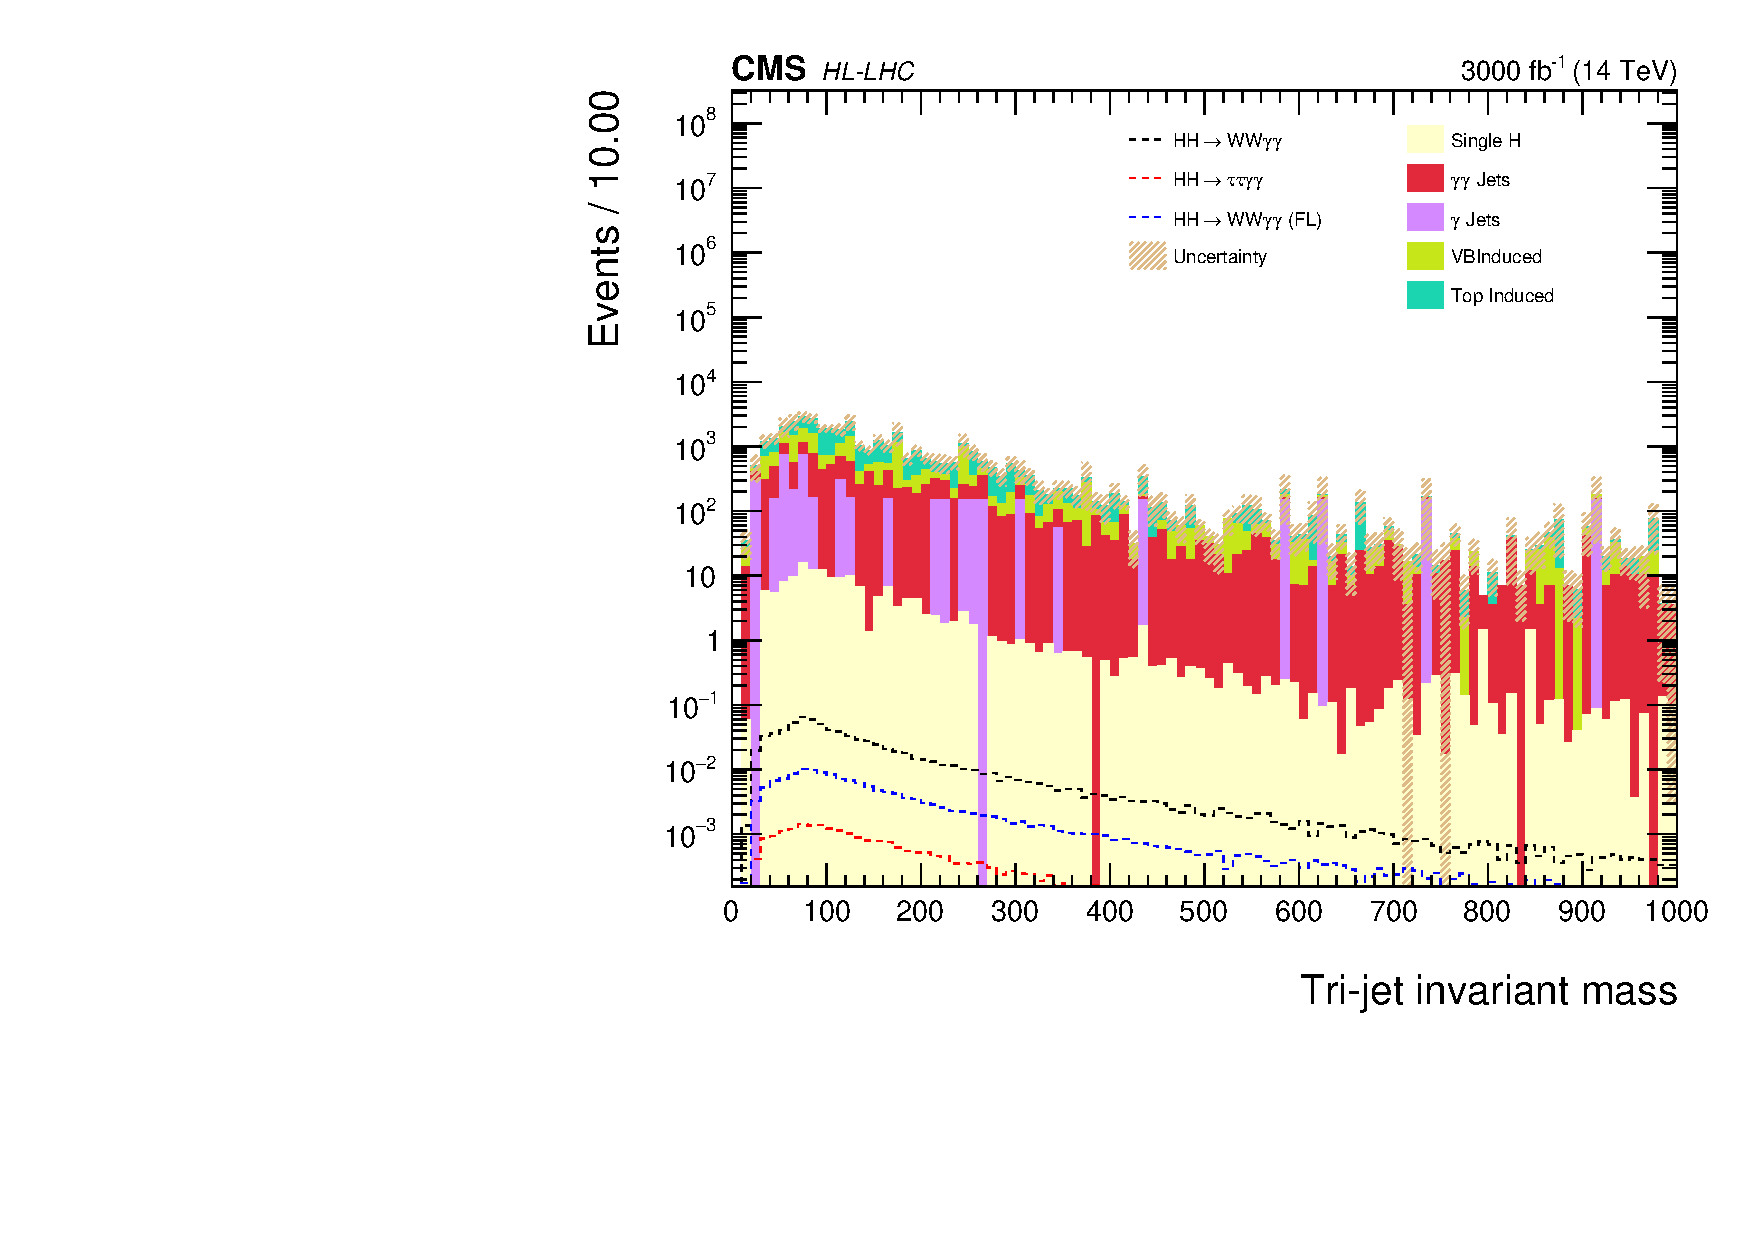
\includegraphics[width=\textwidth]{hasonel_hasthreeJ_mjj_logy.pdf}
        \vspace{-0.5cm}
        \firstsubcaption{$m_{j_1,j_2}$}
    \end{subfigure}
    \vskip\baselineskip
    \begin{subfigure}[b]{0.475\textwidth}   
        \centering 
        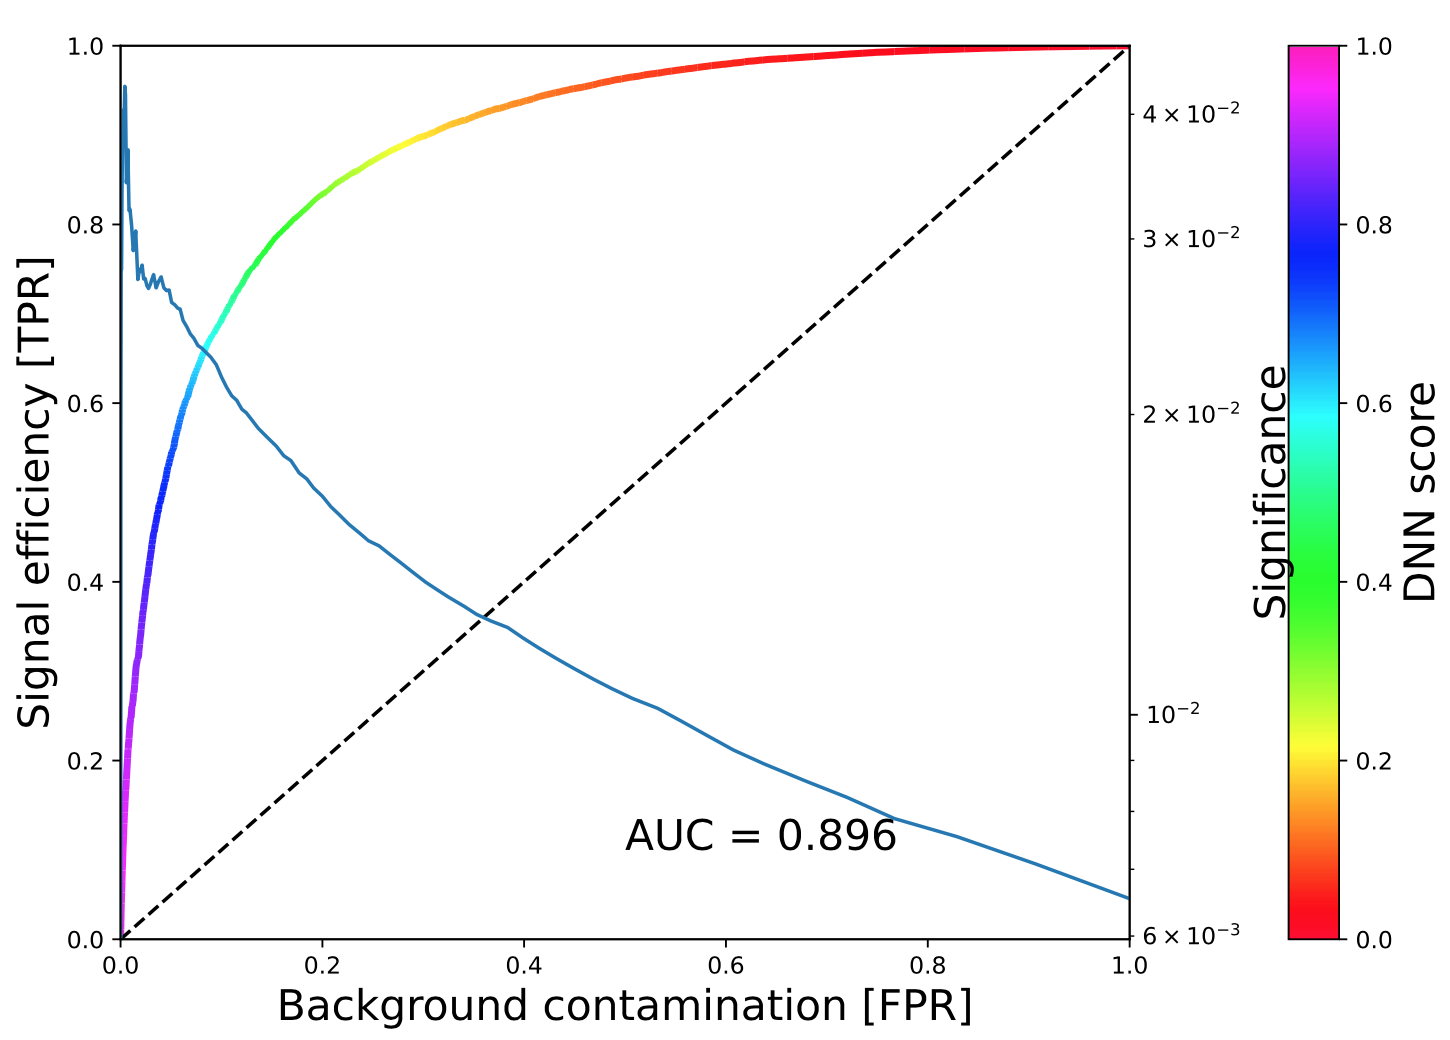
\includegraphics[width=\textwidth]{SLodd_training_roc.png}
        \vspace{-0.5cm}
        \firstsubcaption{Odd training}
    \end{subfigure}
    \hfill
    \begin{subfigure}[b]{0.475\textwidth}   
        \centering 
        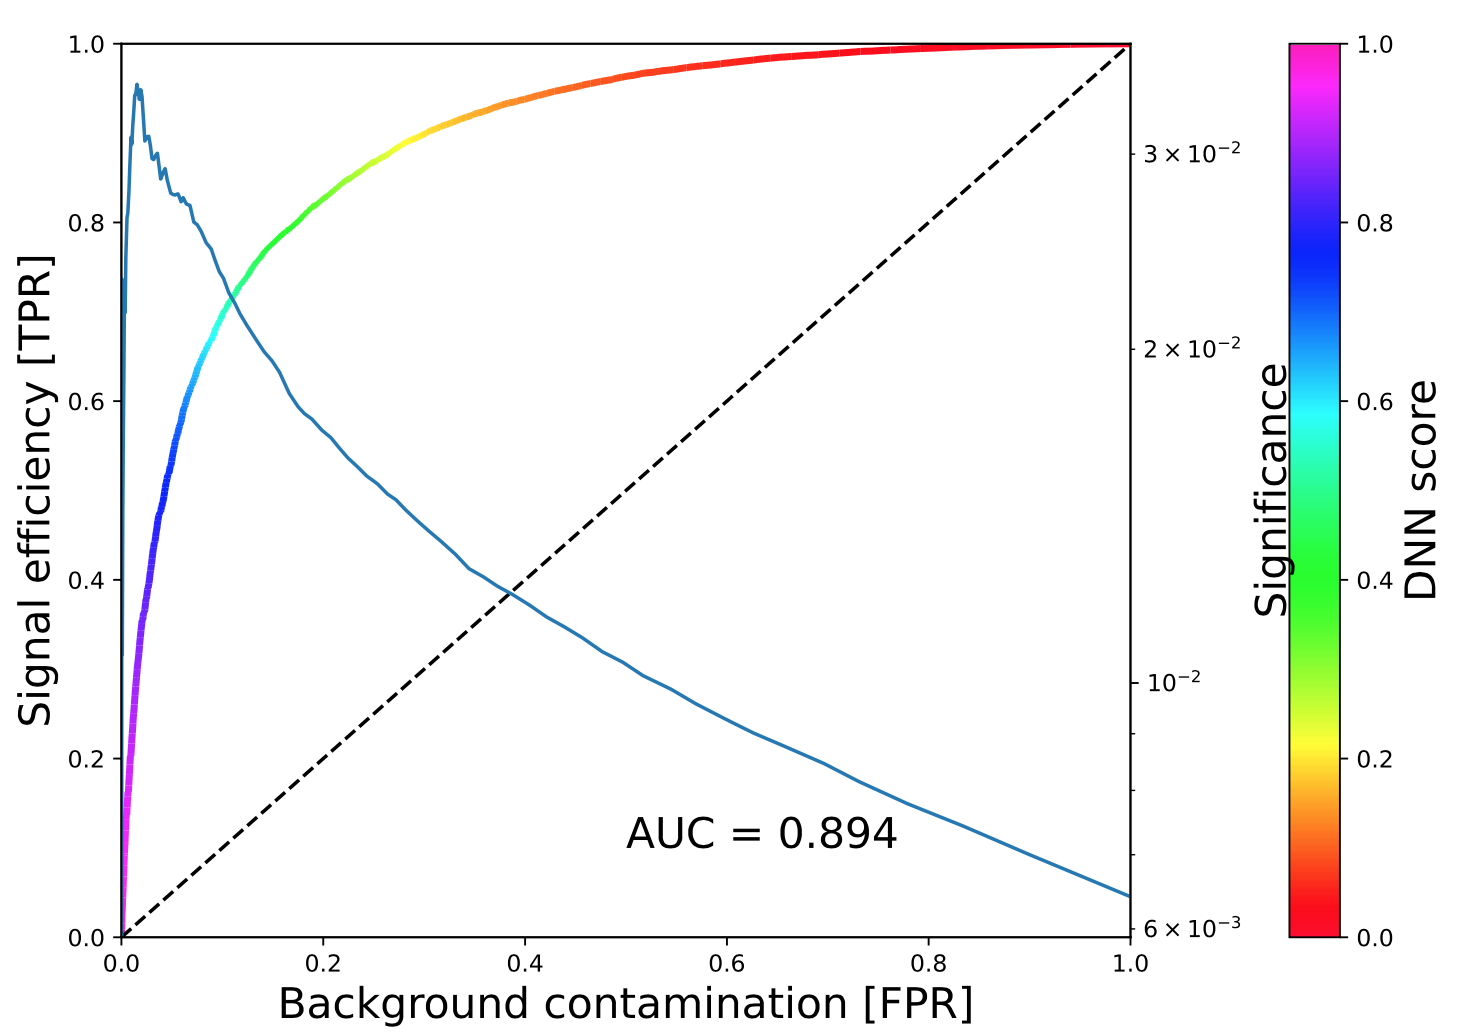
\includegraphics[width=\textwidth]{SLeven_training_roc.png}
        \vspace{-0.5cm} 
        \firstsubcaption{Even training}   
    \end{subfigure}
    \caption{\small DNN input distributions (a,b,c,d) and the ROC curves (e,f) for the semi-leptonic final state (continued).} 
\end{figure*}
\newpage

\begin{figure*}[h!]
    \centering
    \begin{subfigure}[b]{0.475\textwidth}
        \centering
        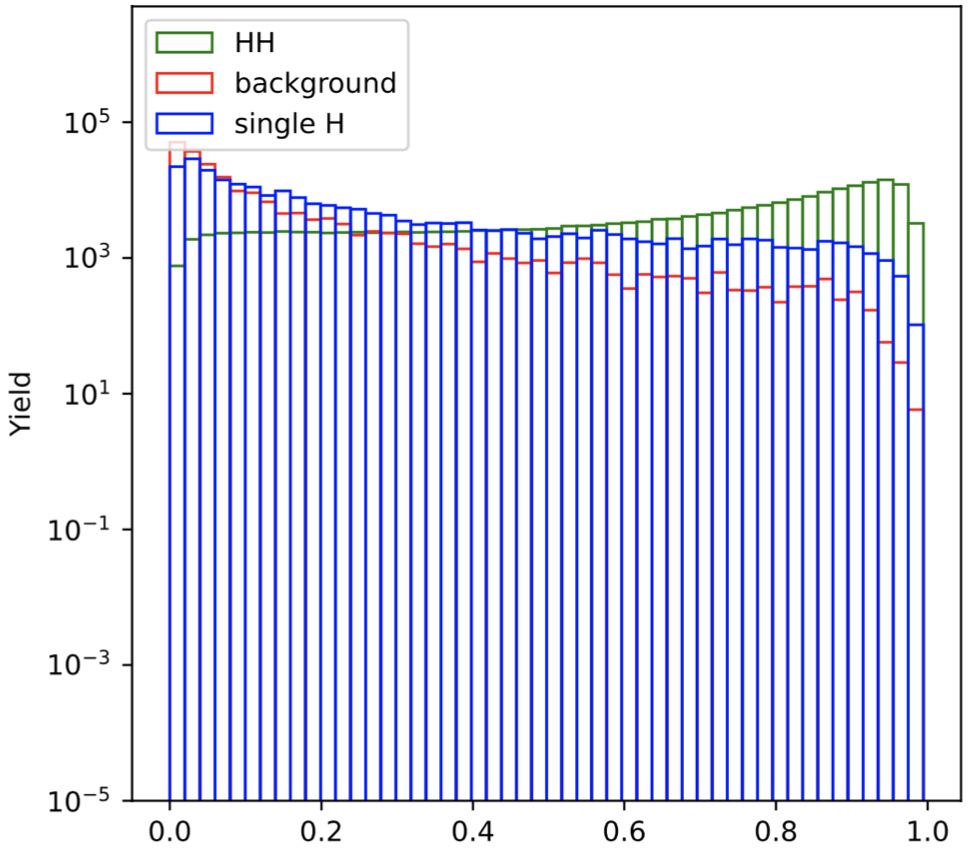
\includegraphics[width=\textwidth]{SLodd-weights.png}
        \vspace{-0.5cm}
        \firstsubcaption{Odd training}
    \end{subfigure}
    \hfill
    \begin{subfigure}[b]{0.475\textwidth}  
        \centering 
        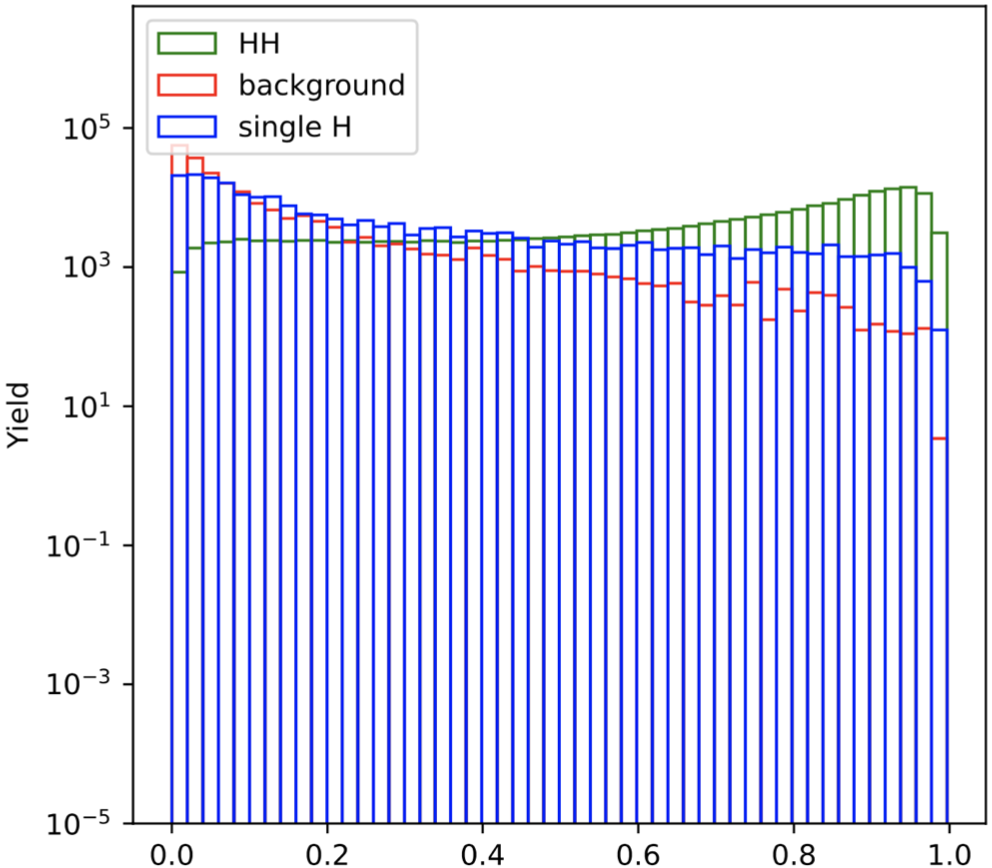
\includegraphics[width=\textwidth]{SLeven-weights.png}
        \vspace{-0.5cm}
        \firstsubcaption{Even training}
    \end{subfigure}
    \caption{\small DNN evaluations for the semi-leptonic channel final state.} 
\end{figure*}

\begin{table}[h!]
    \centering
    \caption{Hyper-parameter settings for the DNN performed for semi-leptonic channel.}
    \begin{tabular}{ l l }
    \hline
    Hyper-parameter & Setting \\
    \hline
    Epochs & 200 \\
    Batch size & 256 \\
    Learning rate & 0.001 \\
    Optimiser & Adam \\
    Loos function & Categorical Cross Entropy \\
    Hidden layer activation functions & ReLU \\
    Output layer activation function & sigmoid \\
    \hline
    \end{tabular}
    \label{hasOneL_dnnpars}
\end{table}
\newpage

%%%%%%%%%%%%%%%%%%%%%%%%%%%%%%%%%%%%%%%%%%%%%%%%%%%%
%%%%%%%%%%%%%%%%%%%%%%%%%%%%%%%%%%%%%%%%%%%%%%%%%%%%
%%%%%%%%%%%%%%%%%%%%%%%%%%%%%%%%%%%%%%%%%%%%%%%%%%%%

\section*{APPENDIX A.4}
\vglue6pt

\begin{table}[h!]
    \centering
    \caption{Cut-flow report showing number of events, before selections, in the semi-leptonic channel and in its categories. Percentages in brackets show the total selection efficiency.}
\begin{tabular}{ |l|c|c| }
    \hline
    Samples                                & No selection & Fully-leptonic final state               \\
    \hline
           $HH \rightarrow WW\gamma\gamma$ &  $4.69e+01$  &  $2.14e-02$ (0.046\%) \\
      $HH \rightarrow WW\gamma\gamma (FL)$ &  $1.12e+01$  &  $3.25e-01$ (2.911\%) \\
     $HH \rightarrow \tau\tau\gamma\gamma$ &  $3.13e+00$  &  $1.64e-02$ (0.525\%) \\
                           \textbf{Signal} &  $1.10e+02$  &  $3.63e-01$ (0.331\%) \\
            $GGH \rightarrow \gamma\gamma$ &  $3.44e+05$  &  $0.00e+00$ (0.000\%) \\
           $VBFH \rightarrow \gamma\gamma$ &  $2.85e+04$  &  $5.38e-02$ (0.000\%) \\
            $ttH \rightarrow \gamma\gamma$ &  $4.18e+03$  &  $2.39e+00$ (0.057\%) \\
             $VH \rightarrow \gamma\gamma$ &  $1.63e+04$  &  $3.03e+00$ (0.019\%) \\
                                     $THQ$ &  $6.16e+02$  &  $7.81e-02$ (0.013\%) \\
              $\gamma\gamma + jets 80-Inf$ &  $2.96e+08$  &  $2.87e+02$ (0.000\%) \\
               $\gamma\gamma + jets 40-80$ &  $9.98e+08$  &  $0.00e+00$ (0.000\%) \\
                                  $G+jets$ &  $2.99e+09$  &  $0.00e+00$ (0.000\%) \\
                         $G+jets 20-40GeV$ &  $7.83e+08$  &  $0.00e+00$ (0.000\%) \\
                           $G+jets 20-Inf$ &  $1.17e+10$  &  $0.00e+00$ (0.000\%) \\
                 $W1Jets \rightarrow L\nu$ &  $3.11e+10$  &  $0.00e+00$ (0.000\%) \\
                 $W2Jets \rightarrow L\nu$ &  $8.90e+09$  &  $0.00e+00$ (0.000\%) \\
                 $W3Jets \rightarrow L\nu$ &  $3.80e+09$  &  $0.00e+00$ (0.000\%) \\
                                    $WGJJ$ &  $1.81e+07$  &  $1.00e+01$ (0.000\%) \\
                                 $WGGJets$ &  $5.65e+06$  &  $5.70e+00$ (0.000\%) \\
                                  $DYJets$ &  $1.71e+10$  &  $0.00e+00$ (0.000\%) \\
                                      $ZG$ &  $4.36e+08$  &  $6.20e+02$ (0.000\%) \\
                           $WW(inclusive)$ &  $2.11e+08$  &  $1.91e+01$ (0.000\%) \\
                    $t\bar{t} (inclusive)$ &  $2.59e+09$  &  $5.25e+01$ (0.000\%) \\
                                 $ttGJets$ &  $1.37e+07$  &  $7.83e+01$ (0.001\%) \\
                                    $ttGG$ &  $5.59e+04$  &  $4.89e+00$ (0.009\%) \\
                                     $ttW$ &  $6.76e+05$  &  $2.52e-01$ (0.000\%) \\
                       \textbf{Background} &  $8.10e+10$  &  $1.08e+03$ (0.000\%) \\
    \hline
\end{tabular}
\label{fullyleptonic-cutflow}
\end{table}
\newpage

%%%%%%%%%%%%%%%%%%%%%%%%%%%%%%%%%%%%%%%%%%%%%%%%%%%%
%%%%%%%%%%%%%%%%%%%%%%%%%%%%%%%%%%%%%%%%%%%%%%%%%%%%
%%%%%%%%%%%%%%%%%%%%%%%%%%%%%%%%%%%%%%%%%%%%%%%%%%%%

\section*{APPENDIX A.5}
\vglue6pt

\begin{table}[h!]
    \caption{Input variables used to train single $\tau$ final state DNN.}
    \resizebox{\textwidth}{!}{
    \begin{tabular}{ l | l }
    \hline
    Feature & Description \\
    \hline
    Leading Photon p$_T$ / \mgg & \pt of the leading good photon scaled to diphoton mass. \\
    Leading Photon Energy / \mgg & Energy of the leading good photon scaled to diphoton mass. \\
    Leading Photon $\eta$ & Pseudorapidity of the leading good photon \\
    Leading Photon $\phi$ & Direction in the transverse plane of the leading good photon\\
    Sub-leading Photon p$_T$ / \mgg & \pt of the sub-leading good photon scaled to diphoton mass.\\
    Sub-leading Photon Energy / \mgg & Energy of the sub-leading good photon scaled to diphoton mass. \\
    Sub-leading Photon $\eta$ & Pseudorapidity of the sub-leading good photon\\
    Sub-leading Photon $\phi$ & Direction in the transverse plane of the sub-leading good photon\\
    Leading Tau p$_T$ & \pt of the leading good Tau \\
    Leading Tau $\eta$ & Pseudorapidity of the leading good Tau \\
    Leading Tau $\phi$ & Direction in the transverse plane of the leading good Tau \\
    Leading Tau Energy & Energy of the leading good Tau \\
    Jet Multiplicity & Number of jets in the event (flavour inclusive) \\
    B-tagged jet Multiplicity & Number of b-tagged jets in the event (flavour inclusive) \\
    Leading Jet p$_T$ & \pt of the leading good jet \\
    Leading Jet $\eta$ & Pseudorapidity of the leading good jet \\
    Sub-leading Jet p$_T$ & \pt of the sub-leading good jet \\
    Sub-leading Jet $\eta$ & Pseudorapidity of the sub-leading good jet \\
    MET & Missing transverse energy in the event \\ 
    \hline
    \end{tabular}
    }
    \label{dnninputs_1tau}
\end{table}
\newpage

\begin{figure*}[h!]
    \centering
    \begin{subfigure}[b]{0.475\textwidth}
        \centering
        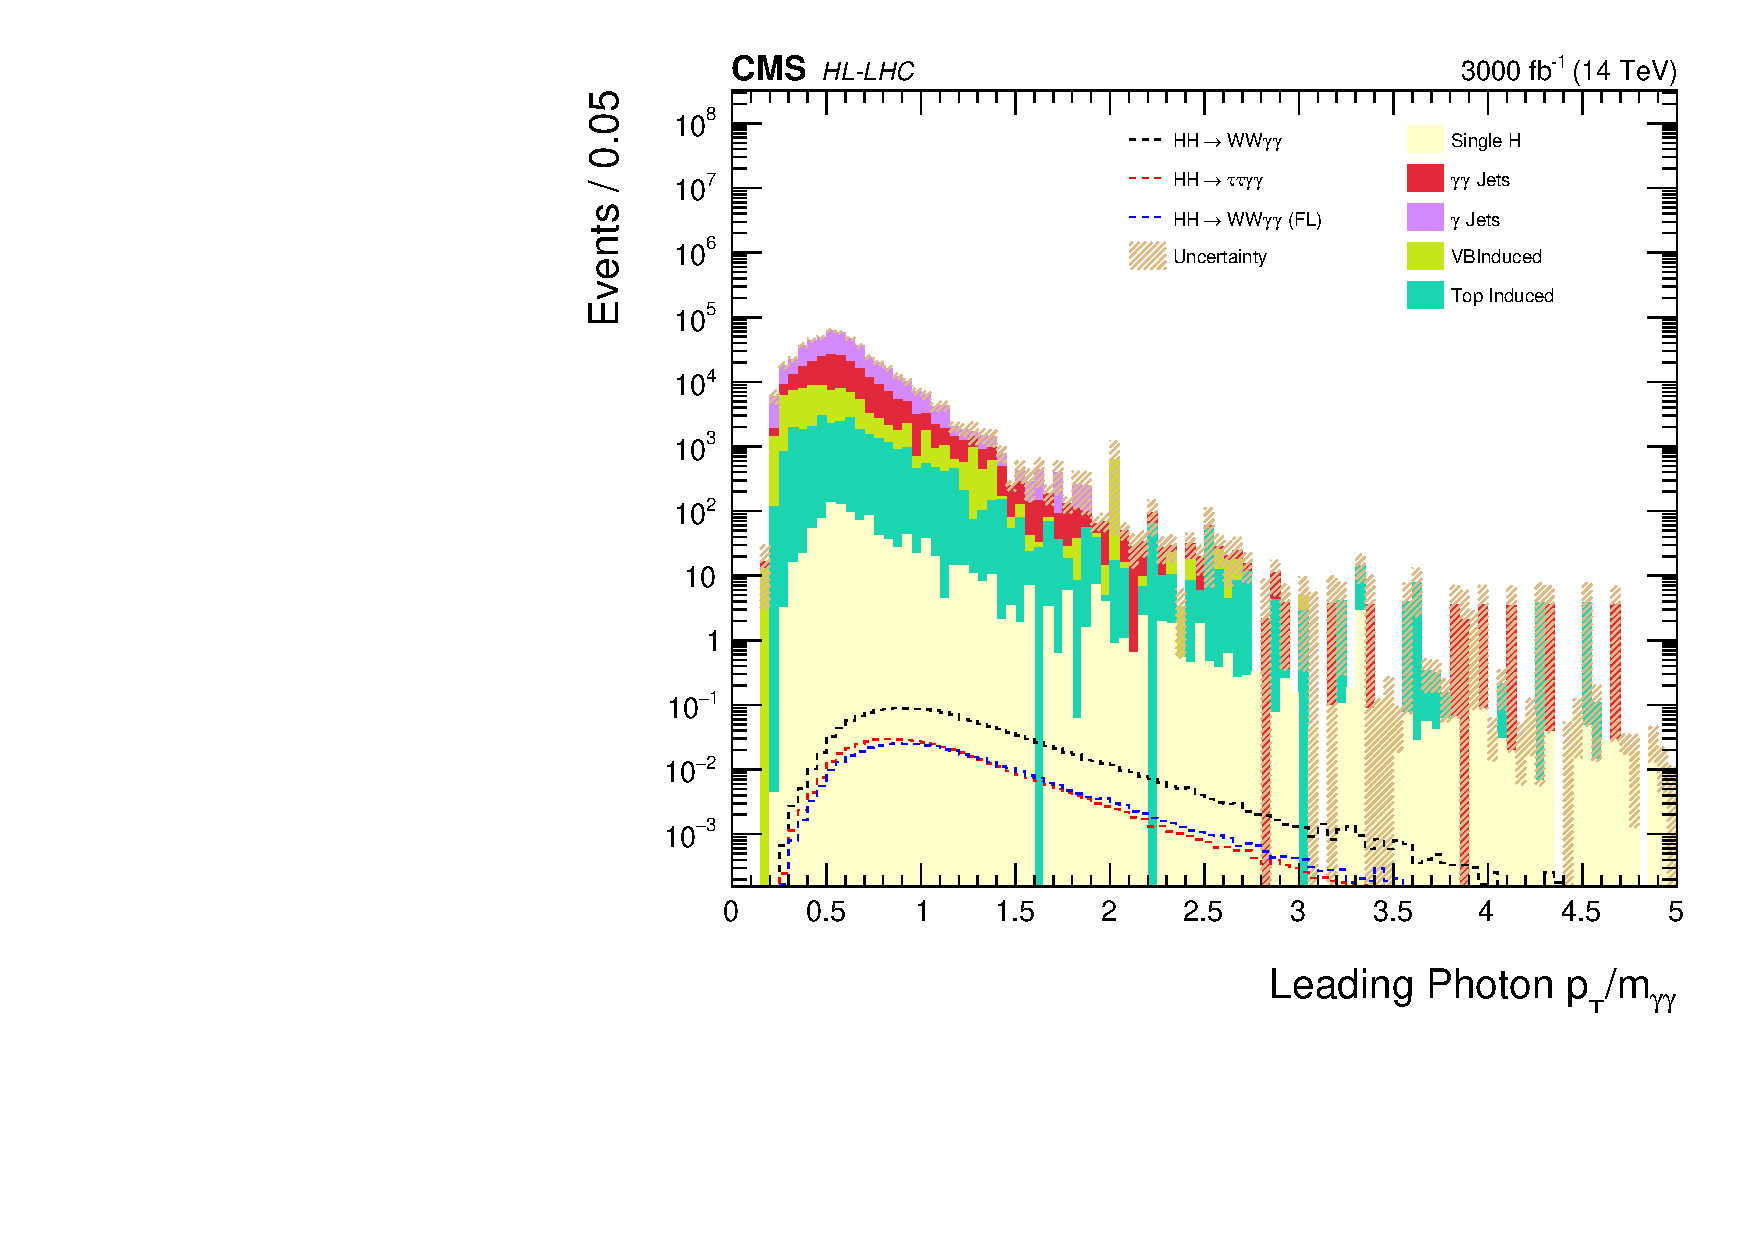
\includegraphics[width=\textwidth]{c3_pt_mgg_logy.pdf}
        \vspace{-0.5cm}
        \firstsubcaption{Leading Photon $p_{T}/m_{\gamma\gamma}$}
    \end{subfigure}
    \hfill
    \begin{subfigure}[b]{0.475\textwidth}  
        \centering 
        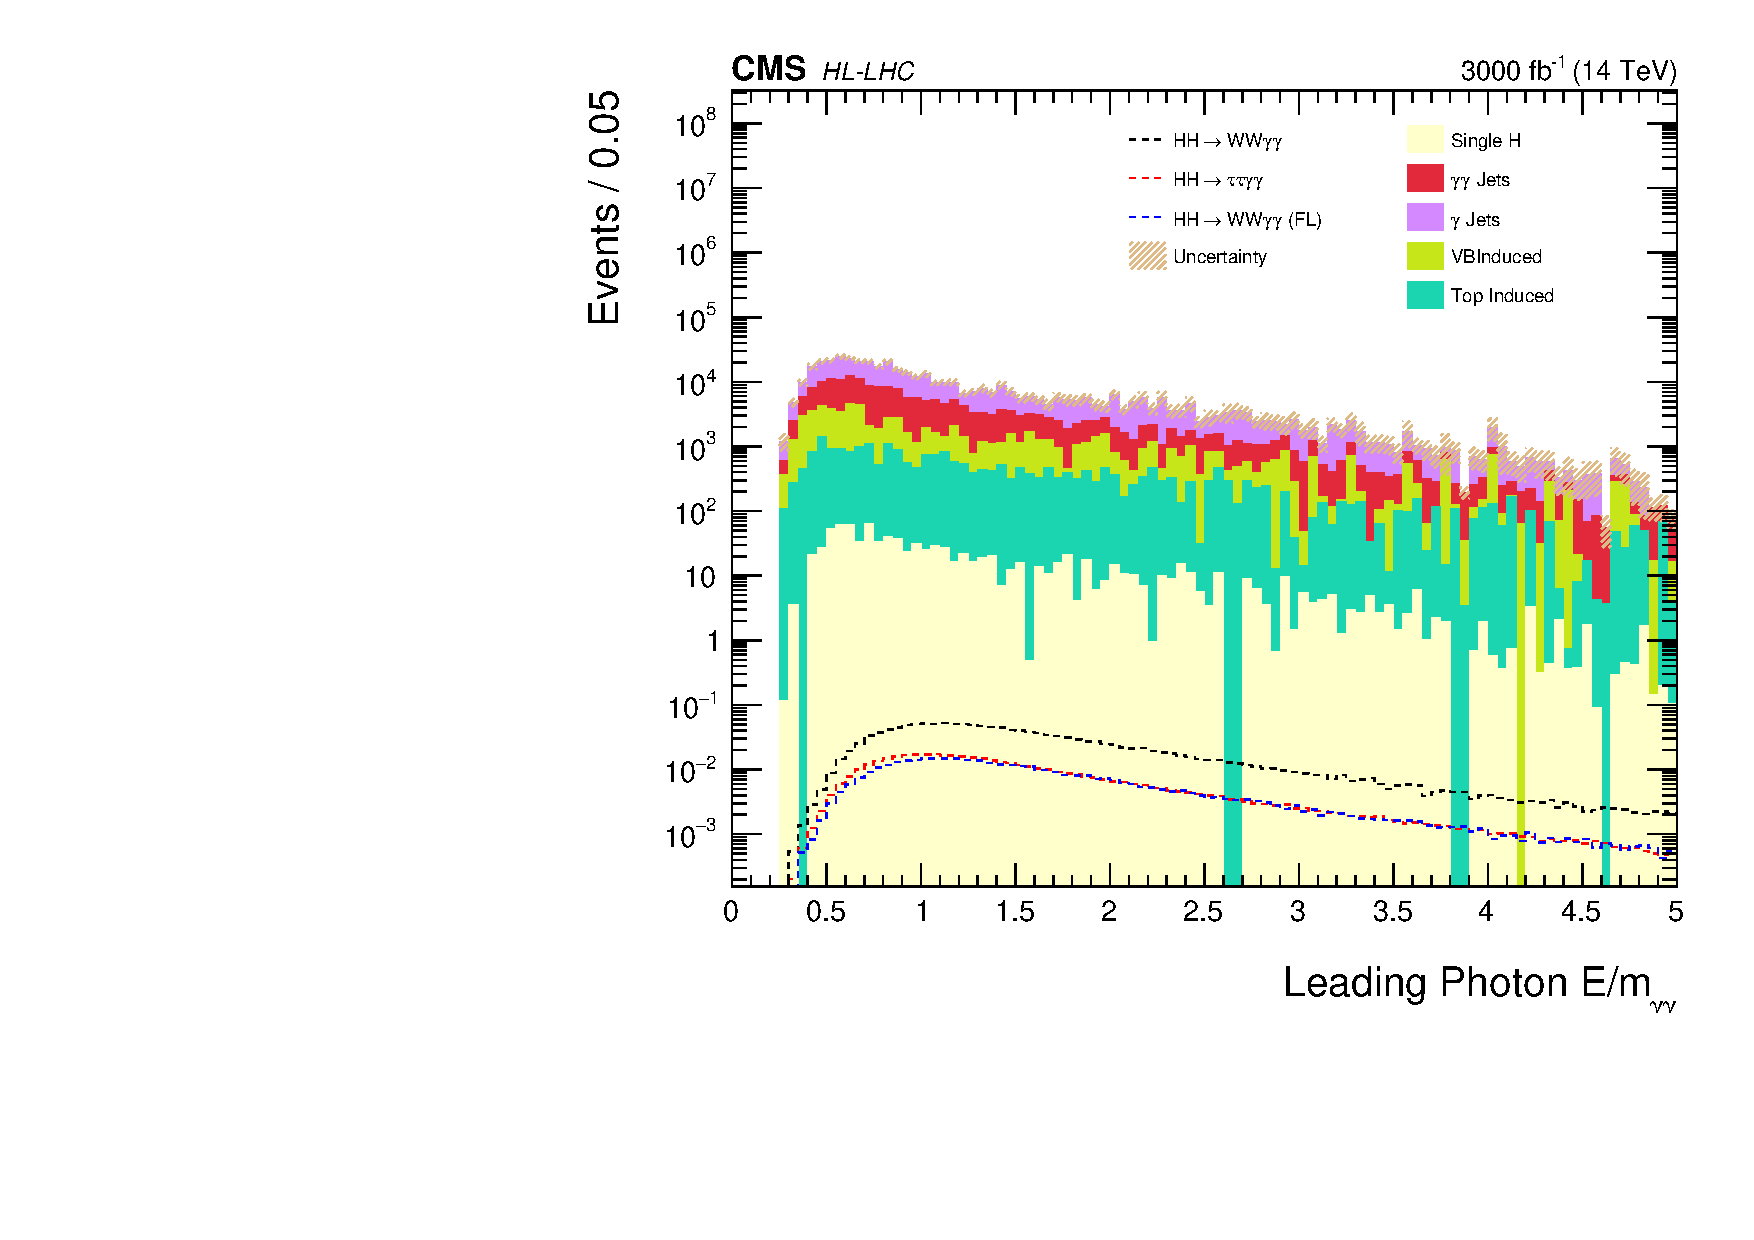
\includegraphics[width=\textwidth]{c3_LE_mgg_logy.pdf}
        \vspace{-0.5cm}
        \firstsubcaption{Leading Photon $E/m_{\gamma\gamma}$}
    \end{subfigure}
    \vskip\baselineskip
    \begin{subfigure}[b]{0.475\textwidth}   
        \centering 
        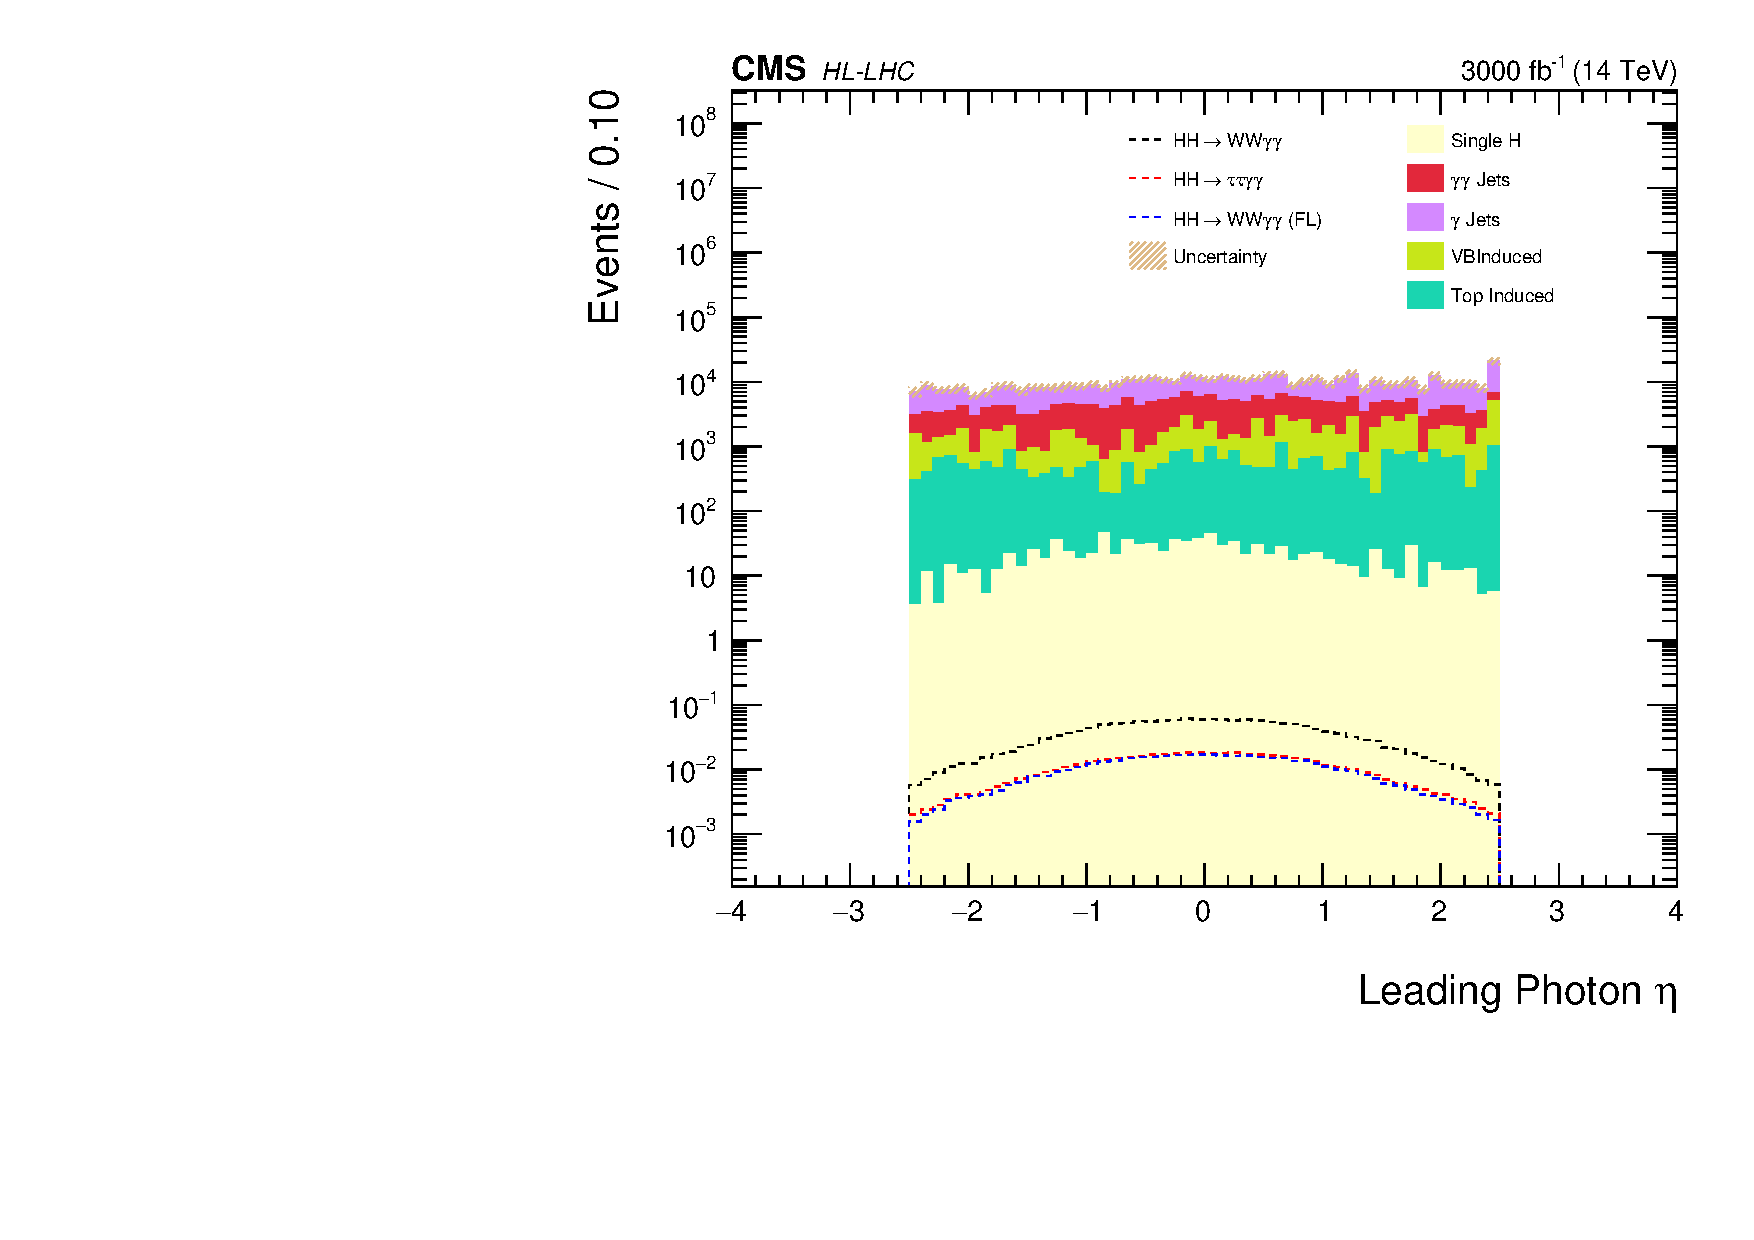
\includegraphics[width=\textwidth]{c3_leadingphoton_eta_logy.pdf}
        \vspace{-0.5cm}
        \firstsubcaption{Leading Photon $\eta$}
    \end{subfigure}
    \hfill
    \begin{subfigure}[b]{0.475\textwidth}   
        \centering 
        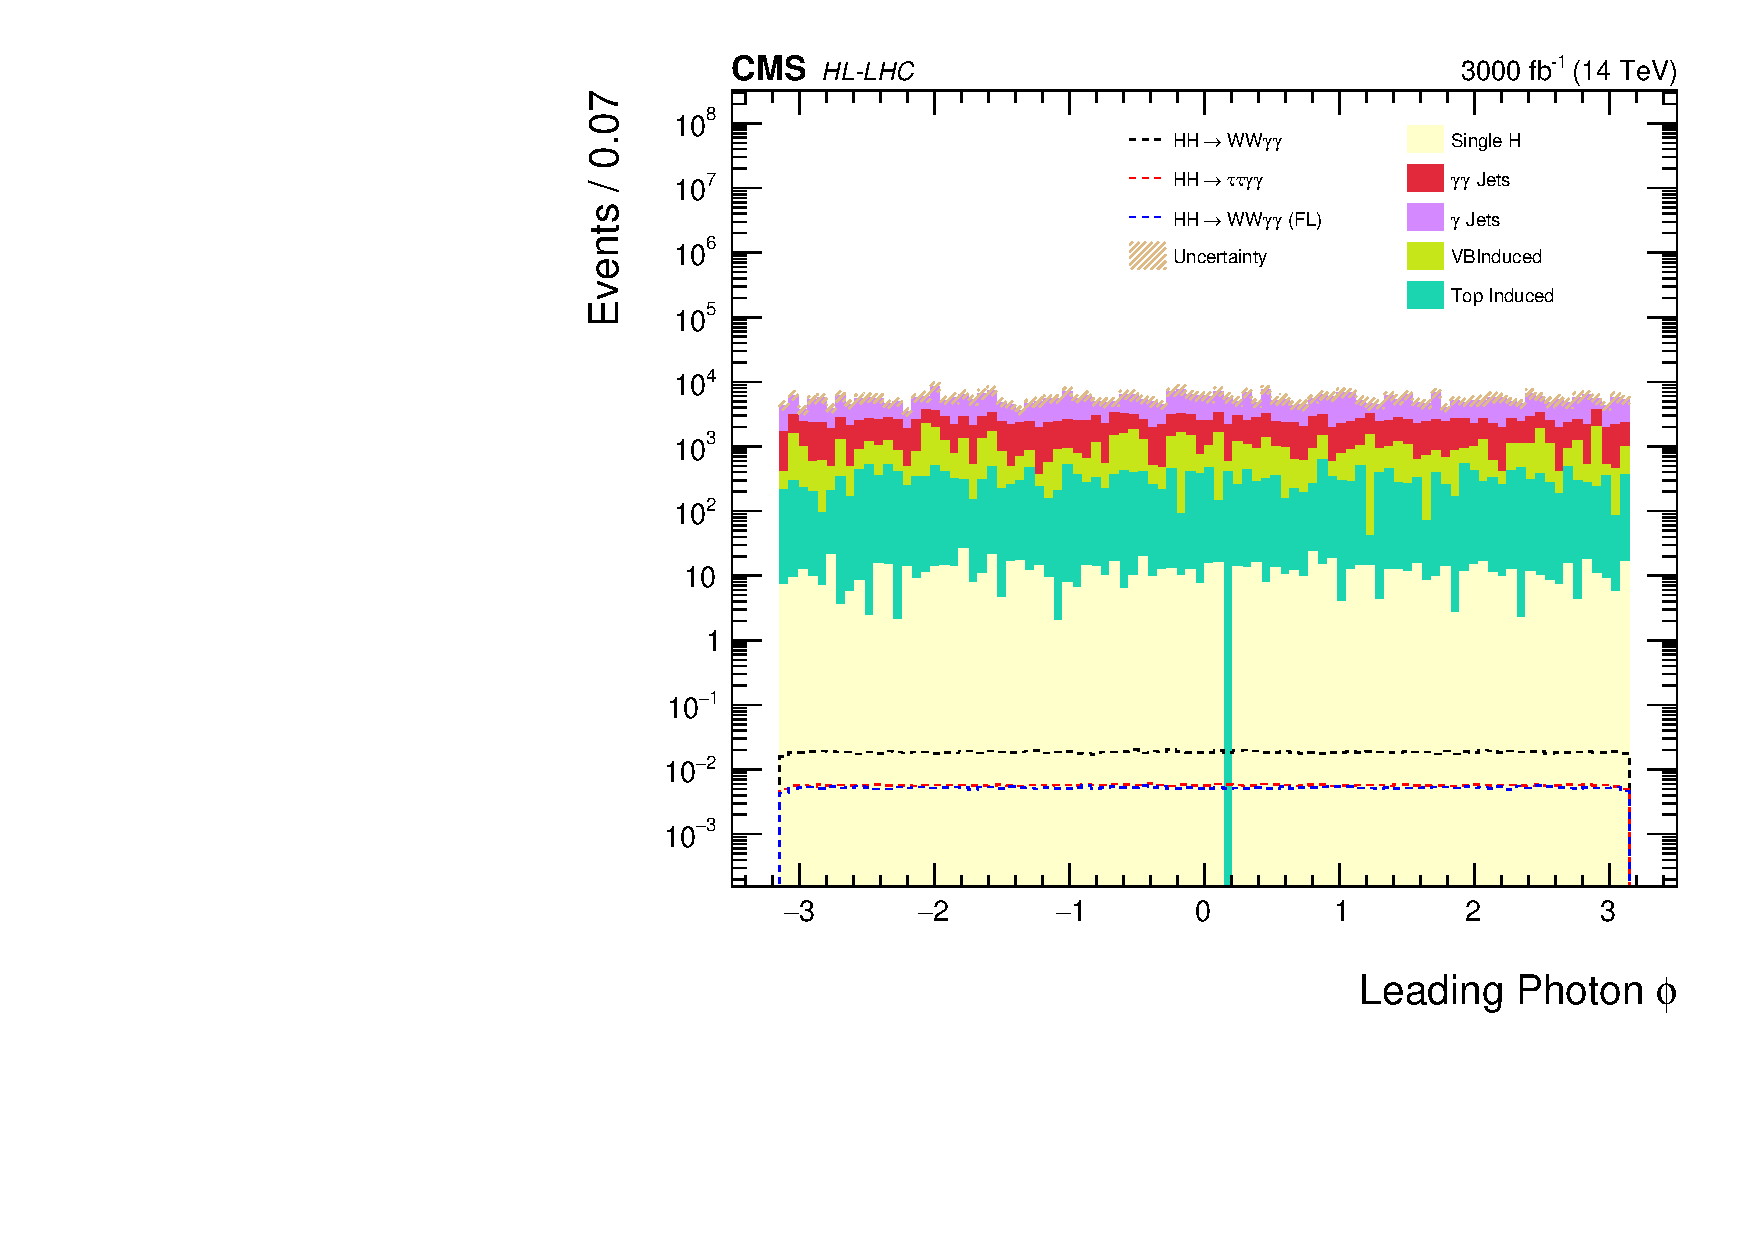
\includegraphics[width=\textwidth]{c3_leadingphoton_phi_logy.pdf}
        \vspace{-0.5cm}
        \firstsubcaption{Leading Photon $\phi$}
    \end{subfigure}
    \vskip\baselineskip
    \begin{subfigure}[b]{0.475\textwidth}   
        \centering 
        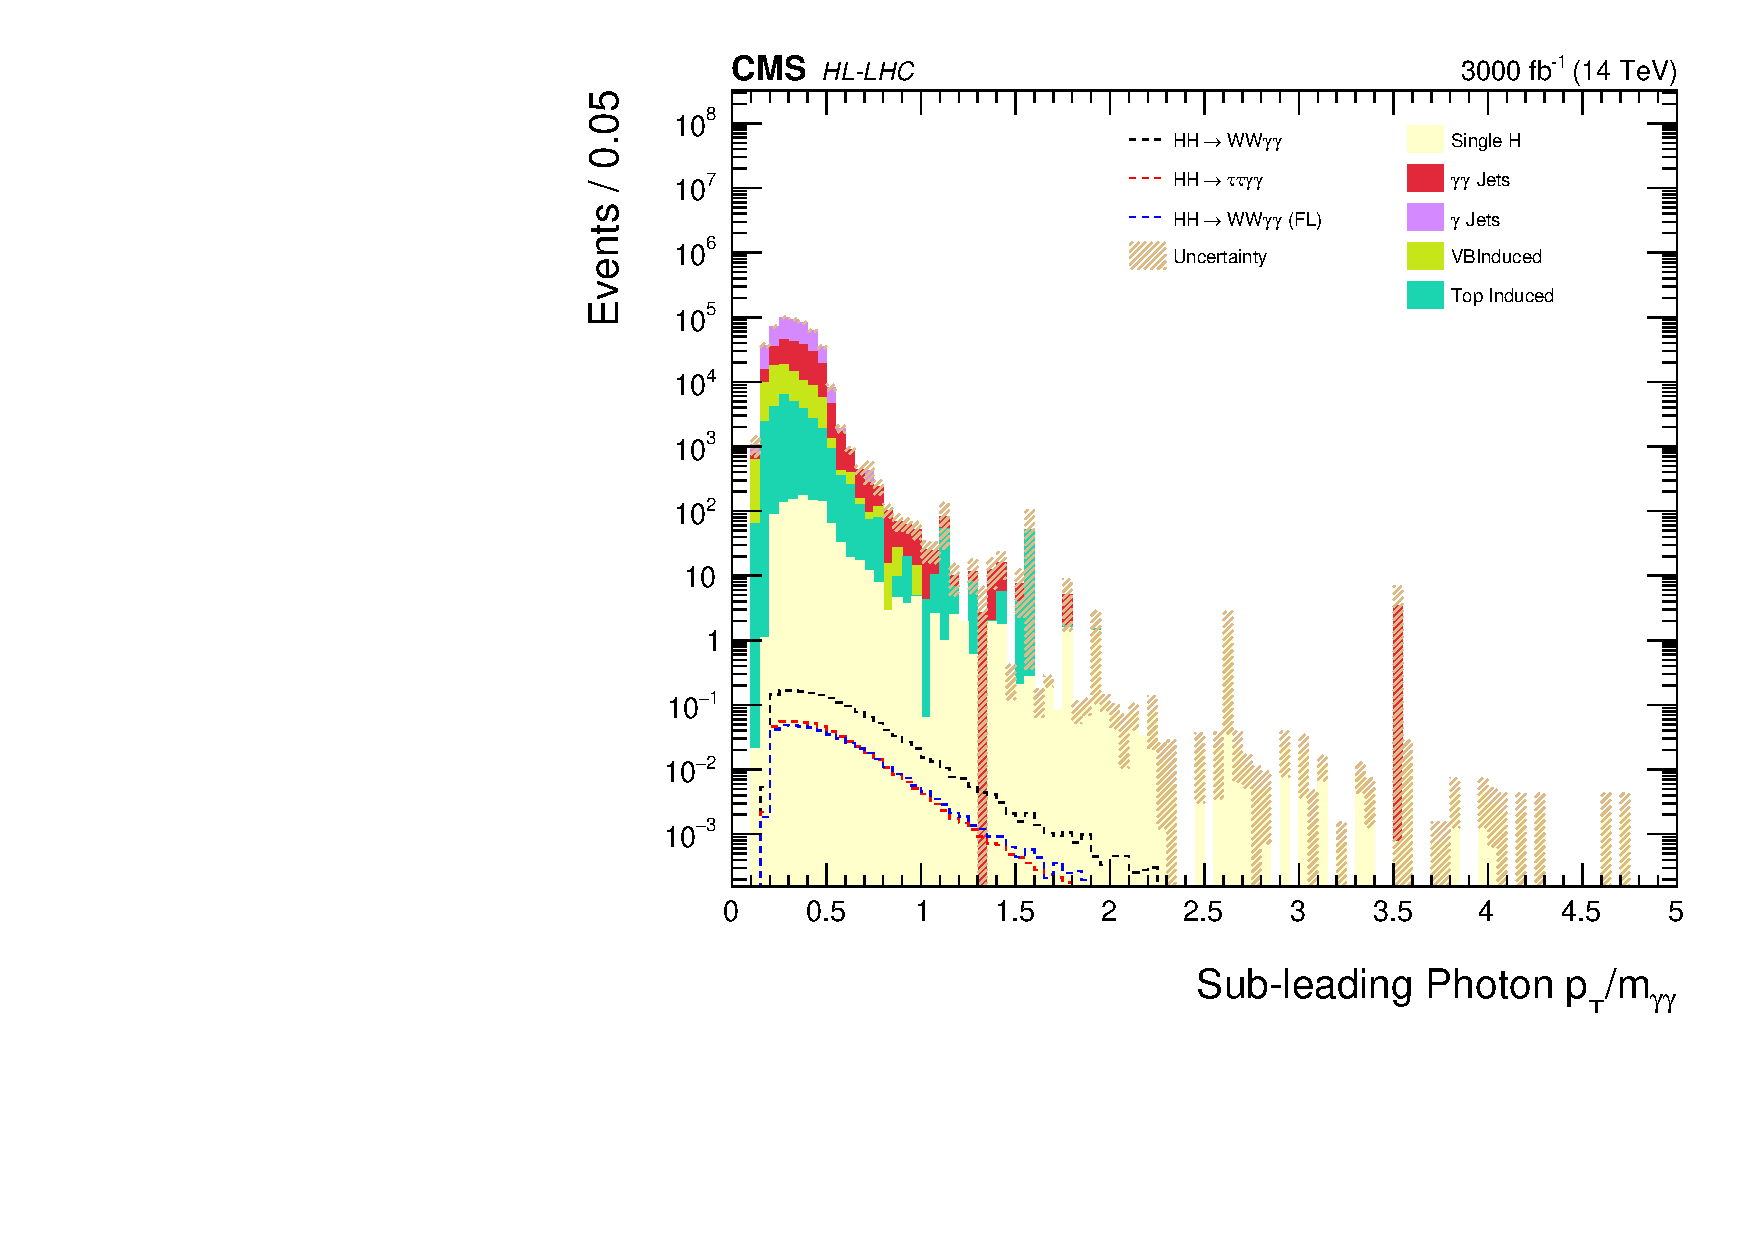
\includegraphics[width=\textwidth]{c3_SLpt_mgg_logy.pdf}
        \vspace{-0.5cm}
        \firstsubcaption{Sub-leading Photon $p_{T}/m_{\gamma\gamma}$}
    \end{subfigure}
    \hfill
    \begin{subfigure}[b]{0.475\textwidth}   
        \centering 
        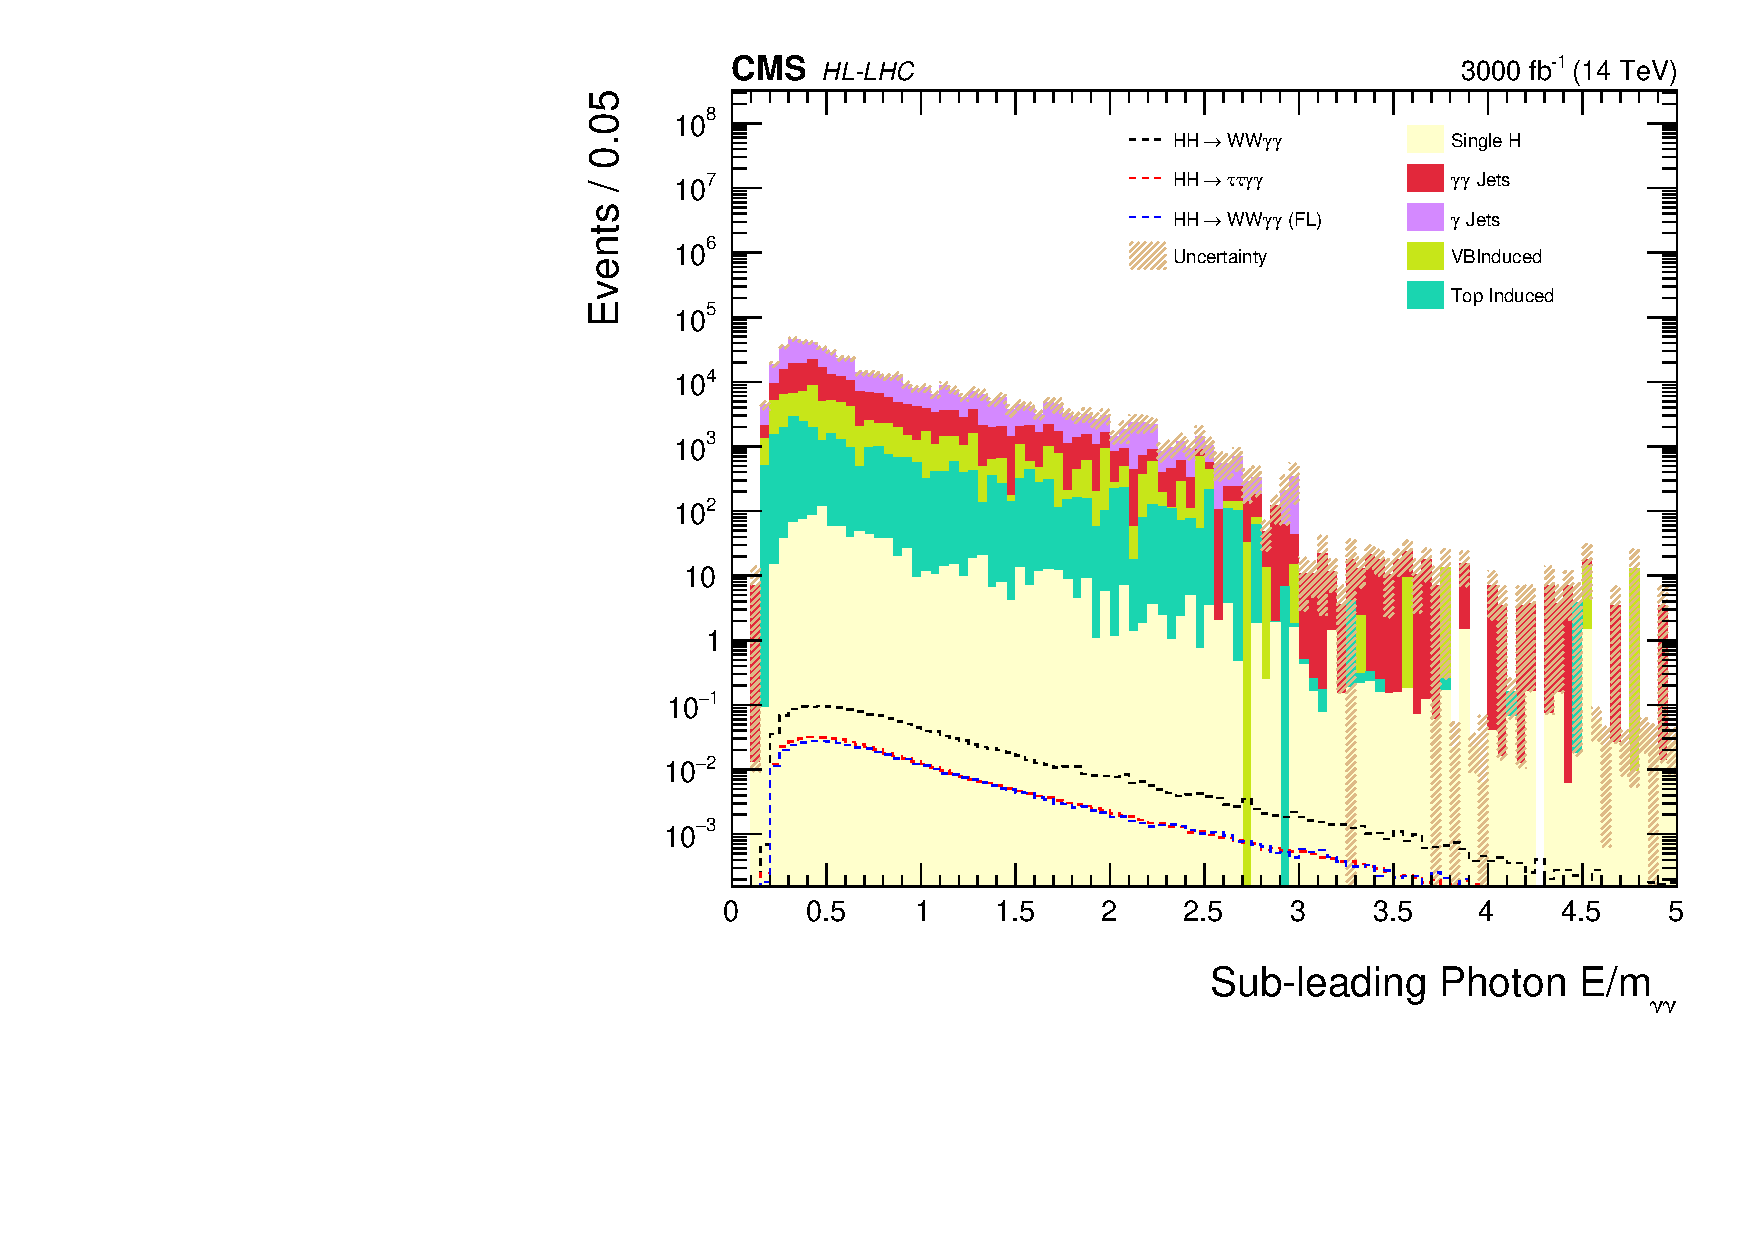
\includegraphics[width=\textwidth]{c3_SLE_mgg_logy.pdf}
        \vspace{-0.5cm}
        \firstsubcaption{Sub-leading Photon $E/m_{\gamma\gamma}$}   
    \end{subfigure}
    \caption{\small DNN input distributions for the single $\tau$ final state.}
    \label{dnninputDists_tau}
\end{figure*}
\newpage

\begin{figure*}[h!]
    \centering
    \begin{subfigure}[b]{0.475\textwidth}
        \centering
        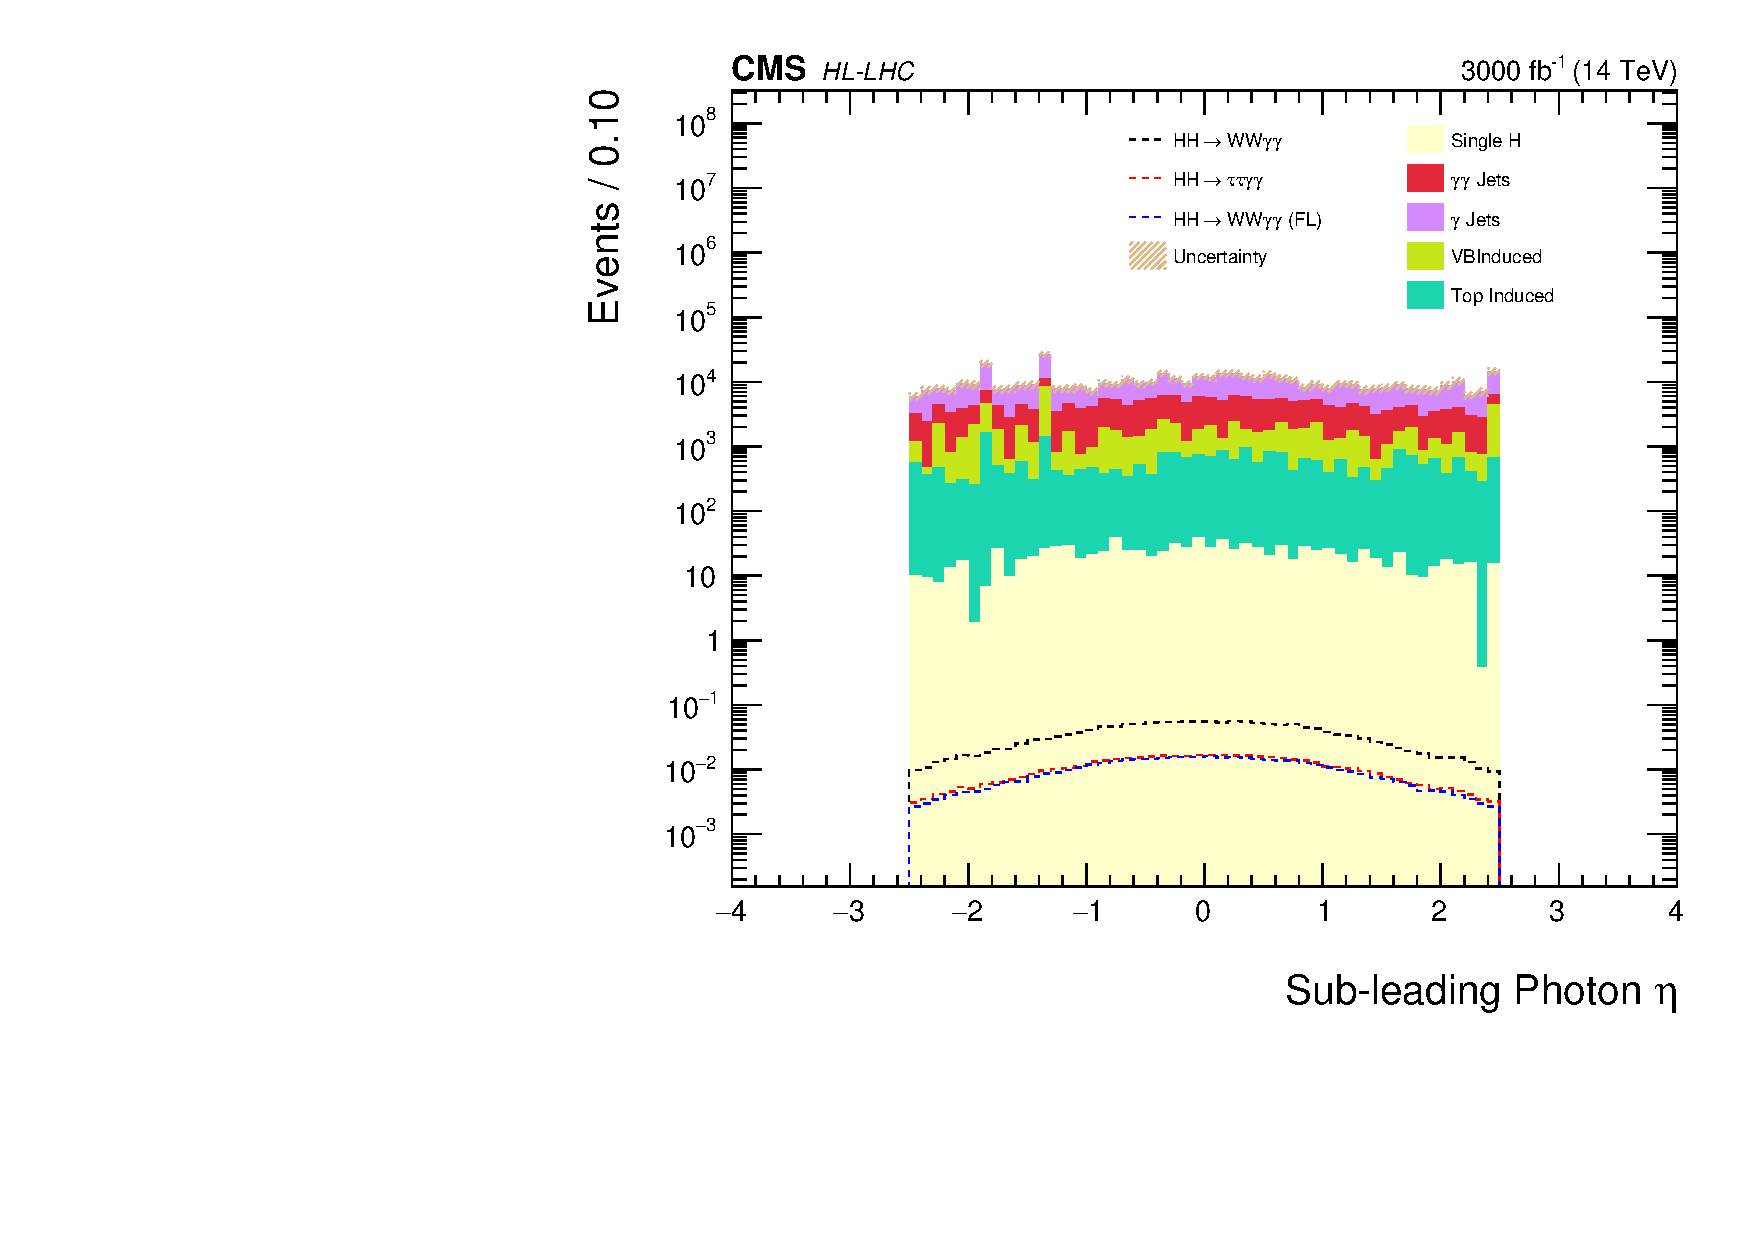
\includegraphics[width=\textwidth]{c3_subleadingphoton_eta_logy.pdf}
        \vspace{-0.5cm}
        \firstsubcaption{Sub-leading Photon $\eta$}
    \end{subfigure}
    \hfill
    \begin{subfigure}[b]{0.475\textwidth}  
        \centering 
        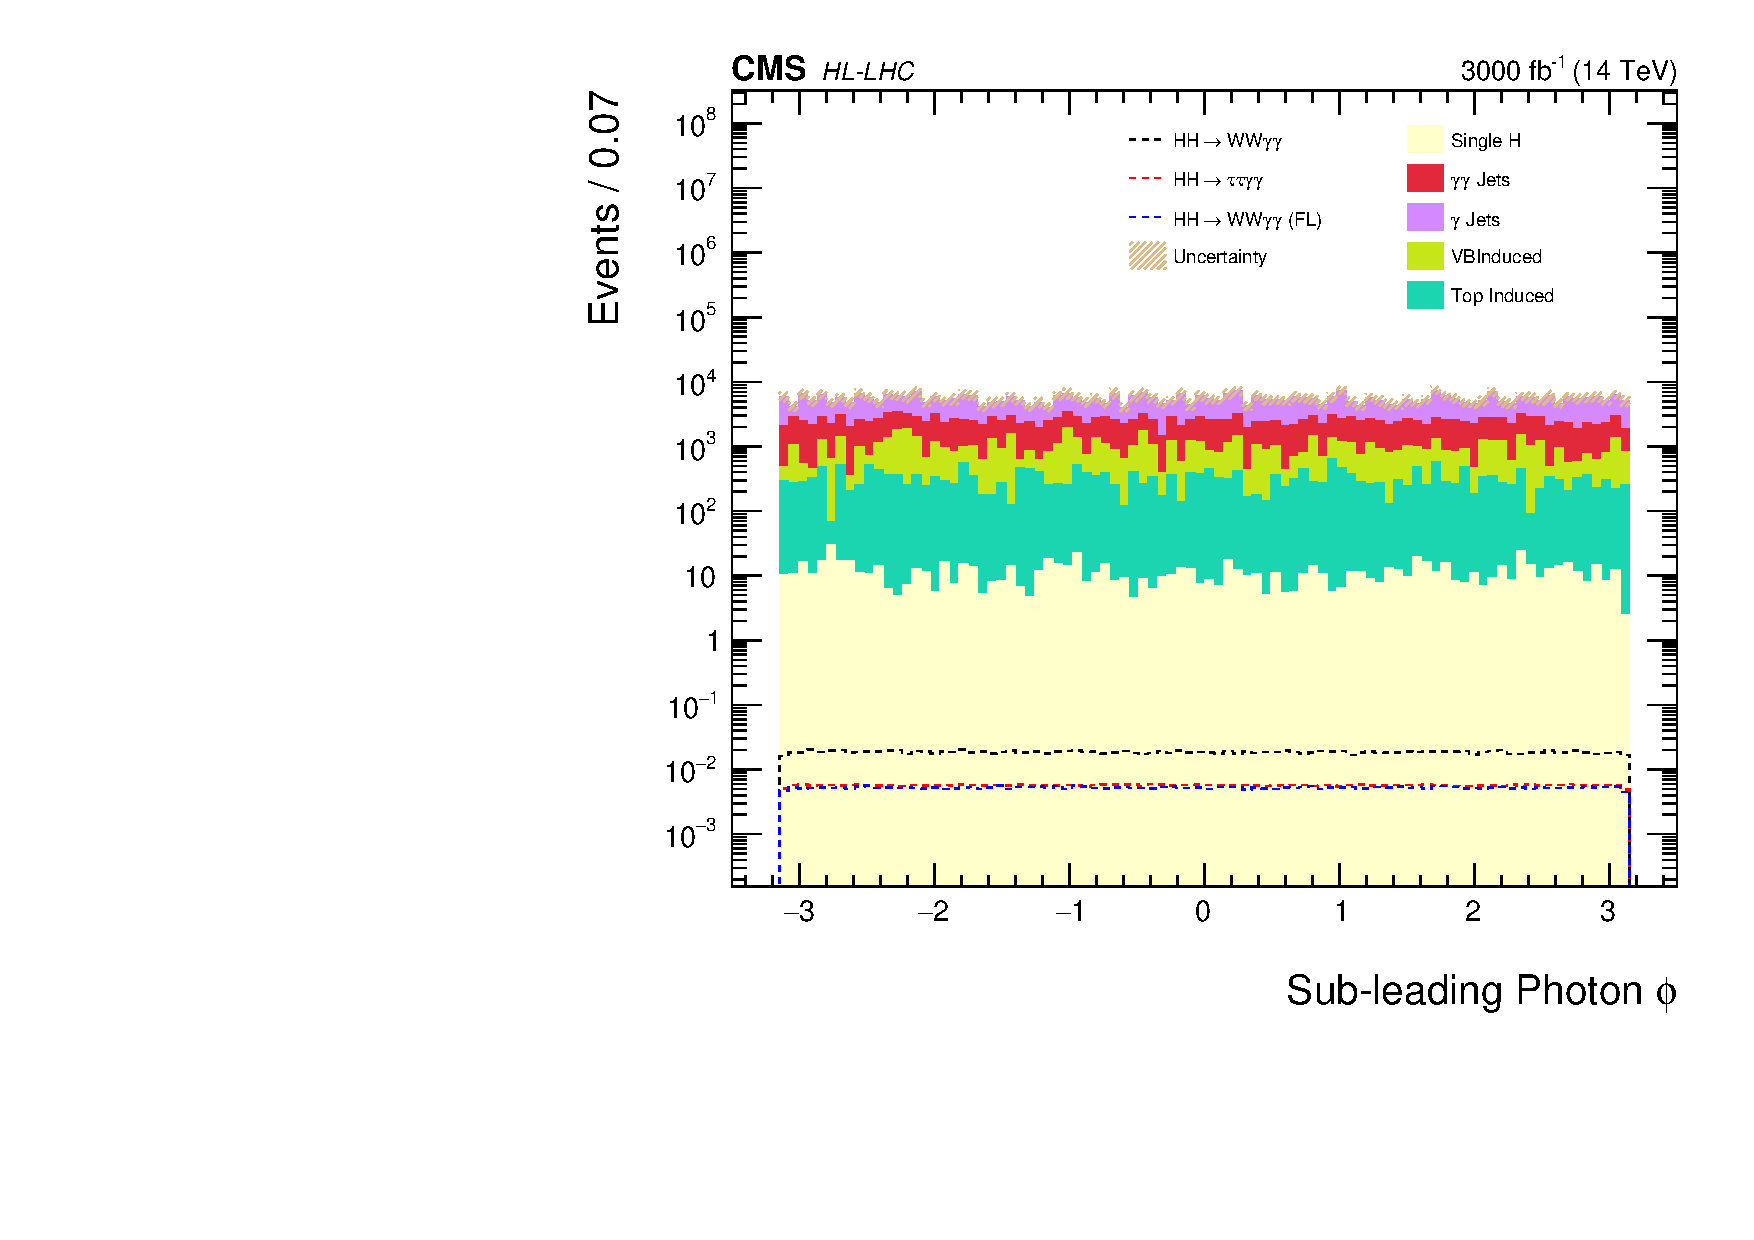
\includegraphics[width=\textwidth]{c3_subleadingphoton_phi_logy.pdf}
        \vspace{-0.5cm}
        \firstsubcaption{Sub-leading Photon $\phi$}
    \end{subfigure}
    \vskip\baselineskip
    \begin{subfigure}[b]{0.475\textwidth}   
        \centering 
        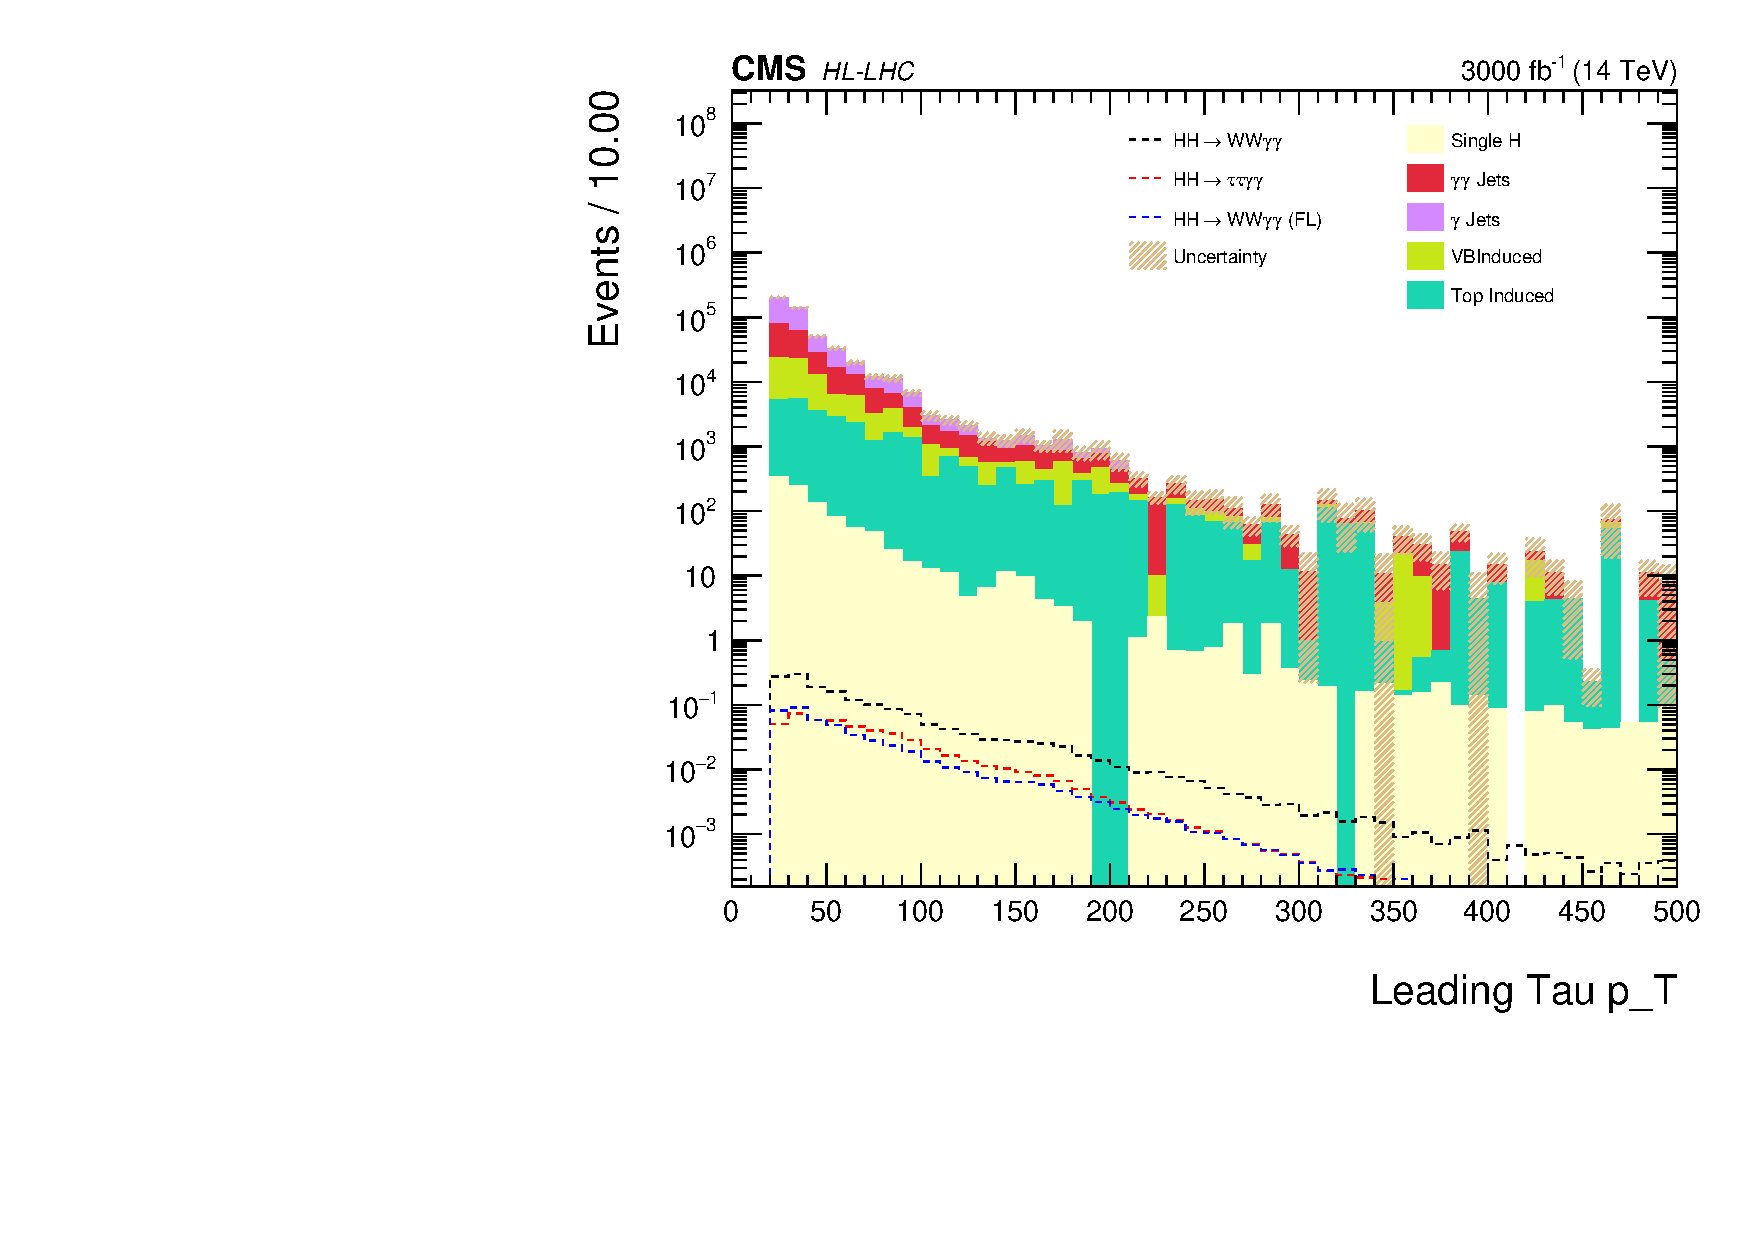
\includegraphics[width=\textwidth]{c3_leadingtau_pt_logy.pdf}
        \vspace{-0.5cm}
        \firstsubcaption{Leading Tau \pt}
    \end{subfigure}
    \hfill
    \begin{subfigure}[b]{0.475\textwidth}   
        \centering 
        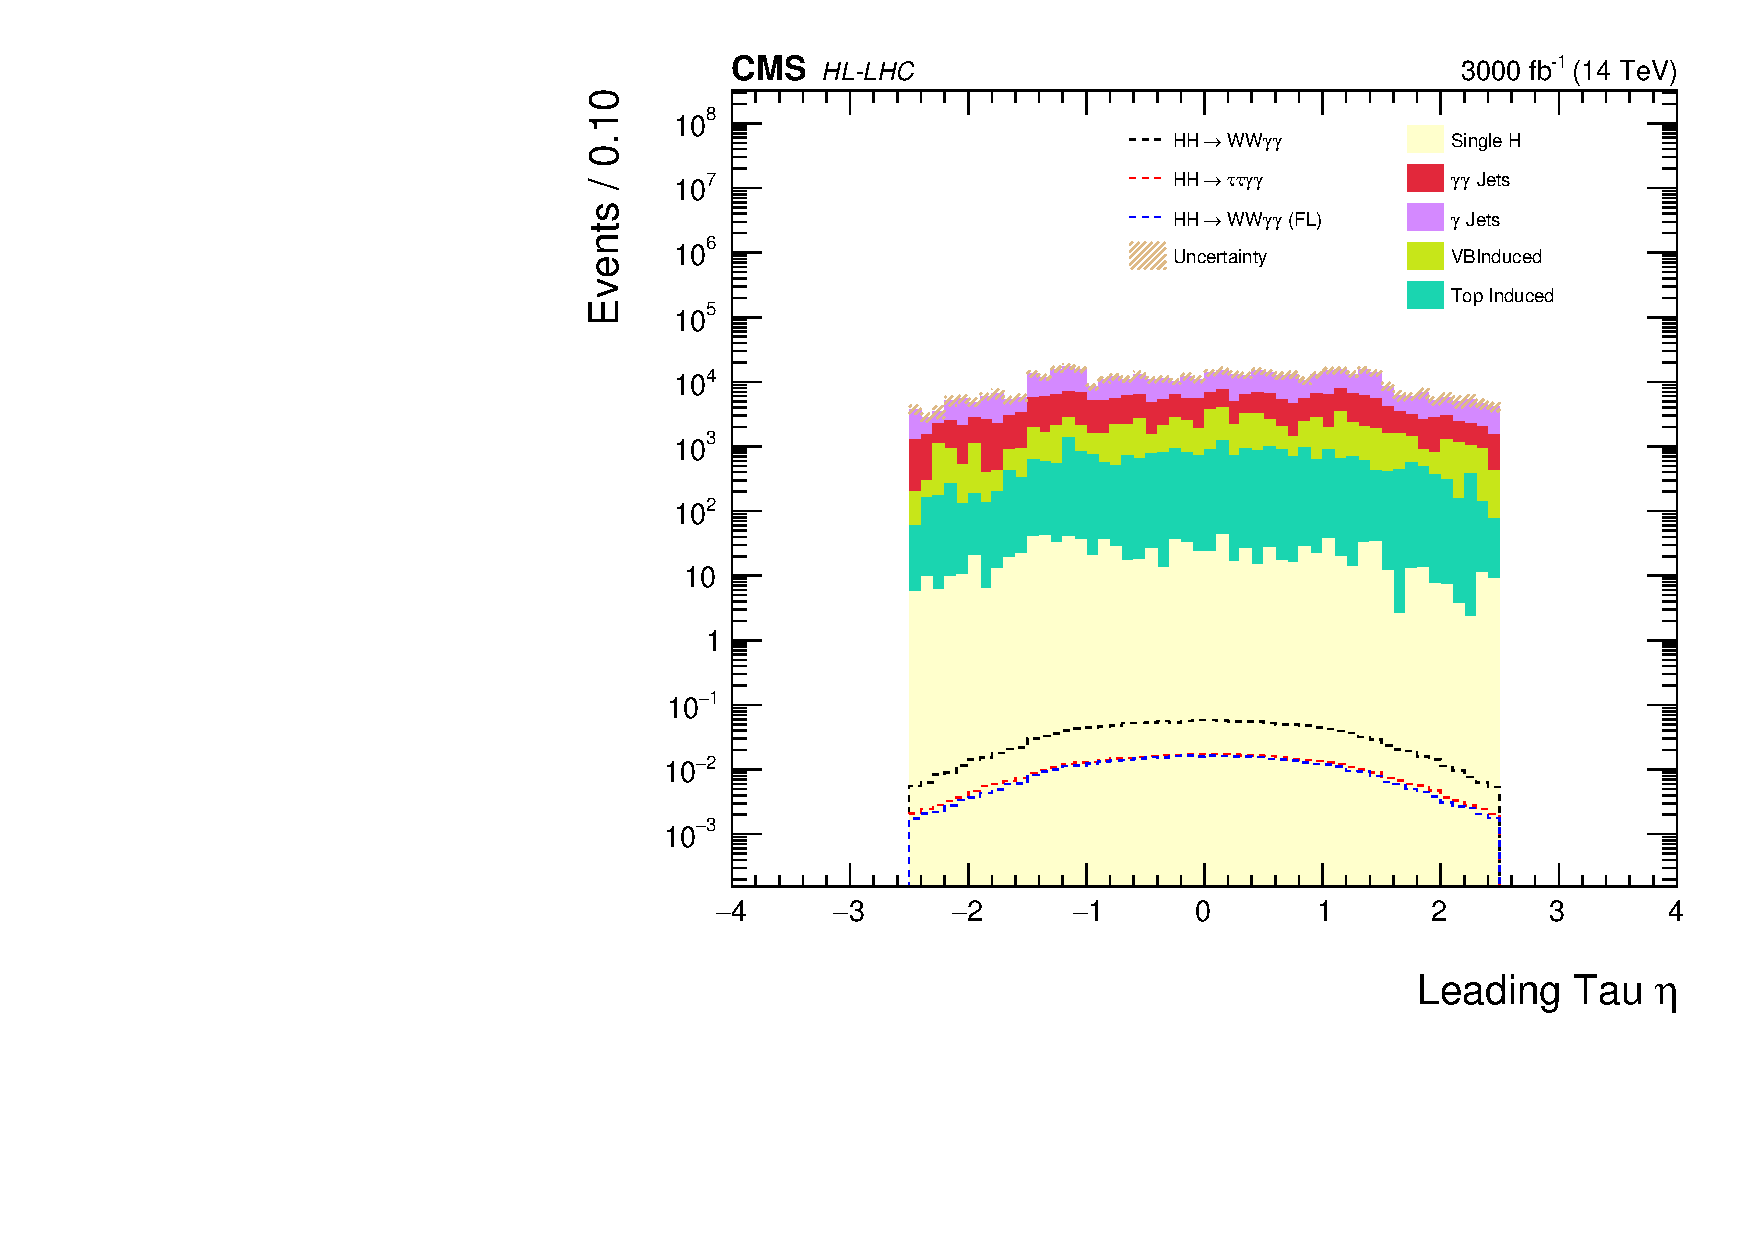
\includegraphics[width=\textwidth]{c3_leadingtau_eta_logy.pdf}
        \vspace{-0.5cm}
        \firstsubcaption{Leading Tau $\eta$}
    \end{subfigure}
    \vskip\baselineskip
    \begin{subfigure}[b]{0.475\textwidth}   
        \centering 
        \includegraphics[width=\textwidth]{c3_leadingtau_phi_logy.pdf}
        \vspace{-0.5cm}
        \firstsubcaption{Leading Tau $\phi$}
    \end{subfigure}
    \hfill
    \begin{subfigure}[b]{0.475\textwidth}   
        \centering 
        \includegraphics[width=\textwidth]{c3_leadingtau_E_logy.pdf}
        \vspace{-0.5cm}
        \firstsubcaption{Leading Tau energy}   
    \end{subfigure}
    \caption{\small DNN input distributions for the single $\tau$ final state (continued).}
\end{figure*}
\newpage

\begin{figure*}[h!]
    \centering
    \begin{subfigure}[b]{0.475\textwidth}
        \centering
        \includegraphics[width=\textwidth]{c3_nJet_logy.pdf}
        \vspace{-0.5cm}
        \firstsubcaption{Jet multiplicity}
    \end{subfigure}
    \hfill
    \begin{subfigure}[b]{0.475\textwidth}  
        \centering 
        \includegraphics[width=\textwidth]{c3_nbJet_logy.pdf}
        \vspace{-0.5cm}
        \firstsubcaption{B-tagged jet multiplicity}
    \end{subfigure}
    \vskip\baselineskip
    \begin{subfigure}[b]{0.475\textwidth}   
        \centering 
        \includegraphics[width=\textwidth]{c3_oneJet_Ljetpt_logy.pdf}
        \vspace{-0.5cm}
        \firstsubcaption{Leading jet \pt}
    \end{subfigure}
    \hfill
    \begin{subfigure}[b]{0.475\textwidth}   
        \centering 
        \includegraphics[width=\textwidth]{c3_oneJet_Ljeteta_logy.pdf}
        \vspace{-0.5cm}
        \firstsubcaption{Leading jet $\eta$}
    \end{subfigure}
    \vskip\baselineskip
    \begin{subfigure}[b]{0.475\textwidth}   
        \centering 
        \includegraphics[width=\textwidth]{c3_twoJet_SLjetpt_logy.pdf}
        \vspace{-0.5cm}
        \firstsubcaption{Sub-leading jet \pt}
    \end{subfigure}
    \hfill
    \begin{subfigure}[b]{0.475\textwidth}   
        \centering 
        \includegraphics[width=\textwidth]{c3_twoJet_SLjeteta_logy.pdf}
        \vspace{-0.5cm}
        \firstsubcaption{Sub-leading jet $\eta$}   
    \end{subfigure}
    \caption{\small DNN input distributions for the single $\tau$ final state (continued).}
\end{figure*}
\newpage

\begin{figure*}[h!]
    \centering
    \begin{subfigure}[b]{0.475\textwidth}
        \centering
        \includegraphics[width=\textwidth]{c3_met_logy.pdf}
        \vspace{-0.5cm}
        \firstsubcaption{$E_T^{miss}$}
    \end{subfigure}
    \vskip\baselineskip
    \begin{subfigure}[b]{0.475\textwidth}  
        \centering 
        \includegraphics[width=\textwidth]{roc-tau-odd.png}
        \vspace{-0.5cm}
        \firstsubcaption{Odd ROC curve}
    \end{subfigure}
    \hfill
    \begin{subfigure}[b]{0.475\textwidth}   
        \centering 
        \includegraphics[width=\textwidth]{roc-tau-even.png}
        \vspace{-0.5cm}
        \firstsubcaption{Even ROC curve}
    \end{subfigure}
    \vskip\baselineskip
    \begin{subfigure}[b]{0.475\textwidth}   
        \centering 
        \includegraphics[width=\textwidth]{onetau-odd-weights.png}
        \vspace{-0.5cm}
        \firstsubcaption{Odd training weight}
    \end{subfigure}
    \hfill
    \begin{subfigure}[b]{0.475\textwidth}   
        \centering 
        \includegraphics[width=\textwidth]{onetau-even-weights.png}
        \vspace{-0.5cm}
        \firstsubcaption{Even training weight}
    \end{subfigure}
    \caption{\small DNN input distributions for the single $\tau$ final state (continued) (a), corresponding ROC curves (b,c) and DNN evaluation on odd (d) and even (e) data.}
\end{figure*}
\newpage

\begin{landscape}
\begin{table}
\centering
\caption{Cut-flow report showing number of events, before selections, in the single $\tau$ final state and in its categories. Percentages in brackets show the total selection efficiency.}
\begin{tabular}{ |l|c|c|c|c| }
    \hline
    Samples                                & No Selection                   & Single $\tau$        & DNN Cat. 1        & DNN Cat. 2       \\
    \hline
           $HH \rightarrow WW\gamma\gamma$ &  $4.69e+01$  &   $1.82e+00$ (3.879\%) &  $7.97e-01$ (1.699\%) &  $8.60e-01$ (1.833\%) \\
      $HH \rightarrow WW\gamma\gamma (FL)$ &  $1.12e+01$  &   $4.98e-01$ (4.459\%) &  $1.91e-01$ (1.710\%) &  $2.57e-01$ (2.304\%) \\
     $HH \rightarrow \tau\tau\gamma\gamma$ &  $3.13e+00$  &  $5.24e-01$ (16.734\%) &  $2.32e-01$ (7.410\%) &  $2.34e-01$ (7.457\%) \\
                           \textbf{Signal} &  $1.10e+02$  &   $3.19e+00$ (2.908\%) &  $1.44e+00$ (1.310\%) &  $1.43e+00$ (1.303\%) \\
            $GGH \rightarrow \gamma\gamma$ &  $3.44e+05$  &   $6.34e+02$ (0.184\%) &  $1.53e+02$ (0.044\%) &  $8.34e+00$ (0.002\%) \\
           $VBFH \rightarrow \gamma\gamma$ &  $2.85e+04$  &   $7.20e+01$ (0.252\%) &  $3.47e+01$ (0.122\%) &  $3.28e+00$ (0.012\%) \\
            $ttH \rightarrow \gamma\gamma$ &  $4.18e+03$  &   $1.36e+02$ (3.250\%) &  $4.68e+01$ (1.120\%) &  $6.89e+00$ (0.165\%) \\
             $VH \rightarrow \gamma\gamma$ &  $1.63e+04$  &   $1.72e+02$ (1.050\%) &  $6.92e+01$ (0.424\%) &  $2.81e+01$ (0.172\%) \\
                                     $THQ$ &  $6.16e+02$  &   $1.35e+01$ (2.198\%) &  $6.20e+00$ (1.007\%) &  $1.97e+00$ (0.319\%) \\
              $\gamma\gamma + jets 80-Inf$ &  $2.96e+08$  &   $1.42e+05$ (0.048\%) &  $3.58e+04$ (0.012\%) &  $1.82e+03$ (0.001\%) \\
               $\gamma\gamma + jets 40-80$ &  $9.98e+08$  &   $1.99e+03$ (0.000\%) &  $3.46e+02$ (0.000\%) &  $2.82e+01$ (0.000\%) \\
                                  $G+jets$ &  $2.99e+09$  &   $2.10e+05$ (0.007\%) &  $3.33e+04$ (0.001\%) &  $1.49e+03$ (0.000\%) \\
                         $G+jets 20-40GeV$ &  $7.83e+08$  &   $1.12e+04$ (0.001\%) &  $1.64e+02$ (0.000\%) &  $0.00e+00$ (0.000\%) \\
                           $G+jets 20-Inf$ &  $1.17e+10$  &   $4.16e+04$ (0.000\%) &  $1.17e+03$ (0.000\%) &  $0.00e+00$ (0.000\%) \\
                 $W1Jets \rightarrow L\nu$ &  $3.11e+10$  &   $8.04e+03$ (0.000\%) &  $8.04e+02$ (0.000\%) &  $0.00e+00$ (0.000\%) \\
                 $W2Jets \rightarrow L\nu$ &  $8.90e+09$  &   $5.56e+03$ (0.000\%) &  $4.12e+02$ (0.000\%) &  $2.06e+02$ (0.000\%) \\
                 $W3Jets \rightarrow L\nu$ &  $3.80e+09$  &   $6.04e+03$ (0.000\%) &  $1.34e+03$ (0.000\%) &  $6.72e+02$ (0.000\%) \\
                                    $WGJJ$ &  $1.81e+07$  &   $2.00e+03$ (0.011\%) &  $7.63e+02$ (0.004\%) &  $1.71e+02$ (0.001\%) \\
                                 $WGGJets$ &  $5.65e+06$  &   $1.81e+03$ (0.032\%) &  $5.76e+02$ (0.010\%) &  $7.42e+01$ (0.001\%) \\
                                  $DYJets$ &  $1.71e+10$  &   $2.14e+04$ (0.000\%) &  $2.67e+03$ (0.000\%) &  $4.46e+02$ (0.000\%) \\
                                      $ZG$ &  $4.36e+08$  &   $1.52e+04$ (0.003\%) &  $3.76e+03$ (0.001\%) &  $2.63e+02$ (0.000\%) \\
    \hline
\end{tabular}
\label{singletau-cutflow}
\end{table}
\end{landscape}
\newpage

\begin{landscape}
\begin{table}
\centering
\caption{Cut-flow report showing number of events, before selections, in the single $\tau$ final state and in its categories (cont'd).}
\begin{tabular}{ |l|c|c|c|c| }
    \hline
    Samples                                & No Selection                   & Single $\tau$        & DNN Cat. 1        & DNN Cat. 2       \\
    \hline
    $WW(inclusive)$ &  $2.11e+08$  &   $5.65e+02$ (0.000\%) &  $1.66e+02$ (0.000\%) &  $2.34e+01$ (0.000\%) \\
                    $t\bar{t} (inclusive)$ &  $2.59e+09$  &   $2.29e+04$ (0.001\%) &  $5.51e+03$ (0.000\%) &  $4.20e+02$ (0.000\%) \\
                                 $ttGJets$ &  $1.37e+07$  &   $4.50e+03$ (0.033\%) &  $1.30e+03$ (0.009\%) &  $8.62e+01$ (0.001\%) \\
                                    $ttGG$ &  $5.59e+04$  &   $2.47e+02$ (0.441\%) &  $6.72e+01$ (0.120\%) &  $7.81e+00$ (0.014\%) \\
                                     $ttW$ &  $6.76e+05$  &   $2.85e+01$ (0.004\%) &  $6.31e+00$ (0.001\%) &  $2.52e-01$ (0.000\%) \\
                       \textbf{Background} &  $8.10e+10$  &   $4.96e+05$ (0.001\%) &  $8.85e+04$ (0.000\%) &  $5.76e+03$ (0.000\%) \\
    \hline
\end{tabular}
\end{table}
\end{landscape}
\newpage

%%%%%%%%%%%%%%%%%%%%%%%%%%%%%%%%%%%%%%%%%%%%%%%%%%%%
%%%%%%%%%%%%%%%%%%%%%%%%%%%%%%%%%%%%%%%%%%%%%%%%%%%%
%%%%%%%%%%%%%%%%%%%%%%%%%%%%%%%%%%%%%%%%%%%%%%%%%%%%

\section*{APPENDIX A.6}
\vglue6pt

\begin{table}
    \centering
    \caption{Cut-flow report showing number of events, before selections and in the double $\tau$ final state of $HH\rightarrow{\tau\tau\gamma\gamma}$.}
    \begin{tabular}{ |l|c|c| }
    \hline
    Samples                                & noSel                   & Two Taus              \\
    \hline
           $HH \rightarrow WW\gamma\gamma$ &  $4.69e+01$  &  $8.29e-02$ (0.177\%) \\
      $HH \rightarrow WW\gamma\gamma (FL)$ &  $1.12e+01$  &  $2.48e-02$ (0.222\%) \\
     $HH \rightarrow \tau\tau\gamma\gamma$ &  $3.13e+00$  &  $1.10e-01$ (3.495\%) \\
                           \textbf{Signal} &  $1.10e+02$  &  $2.22e-01$ (0.202\%) \\
            $GGH \rightarrow \gamma\gamma$ &  $3.44e+05$  &  $1.39e+00$ (0.000\%) \\
           $VBFH \rightarrow \gamma\gamma$ &  $2.85e+04$  &  $1.08e-01$ (0.000\%) \\
            $ttH \rightarrow \gamma\gamma$ &  $4.18e+03$  &  $7.17e+00$ (0.171\%) \\
             $VH \rightarrow \gamma\gamma$ &  $1.63e+04$  &  $4.29e+00$ (0.026\%) \\
                                     $THQ$ &  $6.16e+02$  &  $3.41e-01$ (0.055\%) \\
              $\gamma\gamma + jets 80-Inf$ &  $2.96e+08$  &  $5.14e+02$ (0.000\%) \\
               $\gamma\gamma + jets 40-80$ &  $9.98e+08$  &  $7.06e+00$ (0.000\%) \\
                                  $G+jets$ &  $2.99e+09$  &  $0.00e+00$ (0.000\%) \\
                         $G+jets 20-40GeV$ &  $7.83e+08$  &  $0.00e+00$ (0.000\%) \\
                           $G+jets 20-Inf$ &  $1.17e+10$  &  $0.00e+00$ (0.000\%) \\
                 $W1Jets \rightarrow L\nu$ &  $3.11e+10$  &  $0.00e+00$ (0.000\%) \\
                 $W2Jets \rightarrow L\nu$ &  $8.90e+09$  &  $0.00e+00$ (0.000\%) \\
                 $W3Jets \rightarrow L\nu$ &  $3.80e+09$  &  $0.00e+00$ (0.000\%) \\
                                    $WGJJ$ &  $1.81e+07$  &  $1.00e+01$ (0.000\%) \\
                                 $WGGJets$ &  $5.65e+06$  &  $8.56e+00$ (0.000\%) \\
                                  $DYJets$ &  $1.71e+10$  &  $2.23e+02$ (0.000\%) \\
                                      $ZG$ &  $4.36e+08$  &  $7.33e+02$ (0.000\%) \\
                           $WW(inclusive)$ &  $2.11e+08$  &  $1.49e+01$ (0.000\%) \\
                    $t\bar{t} (inclusive)$ &  $2.59e+09$  &  $1.05e+03$ (0.000\%) \\
                                 $ttGJets$ &  $1.37e+07$  &  $1.45e+02$ (0.001\%) \\
                                    $ttGG$ &  $5.59e+04$  &  $9.98e+00$ (0.018\%) \\
                                     $ttW$ &  $6.76e+05$  &  $2.52e+00$ (0.000\%) \\
                       \textbf{Background} &  $8.10e+10$  &  $2.73e+03$ (0.000\%) \\
    \hline
    \end{tabular}
    \label{cutflow-doubletau}
\end{table}
\newpage

%%%%%%%%%%%%%%%%%%%%%%%%%%%%%%%%%%%%%%%%%%%%%%%%%%%%
%%%%%%%%%%%%%%%%%%%%%%%%%%%%%%%%%%%%%%%%%%%%%%%%%%%%
%%%%%%%%%%%%%%%%%%%%%%%%%%%%%%%%%%%%%%%%%%%%%%%%%%%%

\section*{APPENDIX A.7}
\vglue6pt

\begin{figure*}[h!]
    \centering
    \begin{subfigure}[b]{0.475\textwidth}
        \centering
        \includegraphics[width=\textwidth]{Inv_mass_gghasOneL_DNN_HL_FIT.pdf}
        \vspace{-0.5cm}
        \firstsubcaption{Cat. 1}
    \end{subfigure}
    \vskip\baselineskip
    \begin{subfigure}[b]{0.475\textwidth}  
        \centering 
        \includegraphics[width=\textwidth]{Inv_mass_gghasOneL_DNN_2_HL_FIT.pdf}
        \vspace{-0.5cm}
        \firstsubcaption{Cat. 2}
    \end{subfigure}
    \hfill
    \begin{subfigure}[b]{0.475\textwidth}   
        \centering 
        \includegraphics[width=\textwidth]{Inv_mass_gghasOneL_DNN_3_HL_FIT.pdf}
        \vspace{-0.5cm}
        \firstsubcaption{Cat. 3}
    \end{subfigure}
    \vskip\baselineskip
    \begin{subfigure}[b]{0.475\textwidth}   
        \centering 
        \includegraphics[width=\textwidth]{Inv_mass_gghasOneL_HL_FIT.pdf}
        \vspace{-0.5cm}
        \firstsubcaption{Semi-leptonic}
    \end{subfigure}
    \hfill
    \begin{subfigure}[b]{0.475\textwidth}   
        \centering 
        \includegraphics[width=\textwidth]{Inv_mass_gghasTwoL_HL_FIT.pdf}
        \vspace{-0.5cm}
        \firstsubcaption{Fully-leptonic}
    \end{subfigure}
    \caption{\small Fitted distributions of semi-leptonic channel (a,b,c) and fully-leptonic (d,e).}
\label{allfits}
\end{figure*}

\begin{figure*}[h!]
    \centering
    \begin{subfigure}[b]{0.475\textwidth}
        \centering
        \includegraphics[width=\textwidth]{Mgg_c3_HL_FIT.pdf}
        \vspace{-0.5cm}
        \firstsubcaption{Single $\tau$}
    \end{subfigure}
    \hfill
    \begin{subfigure}[b]{0.475\textwidth}  
        \centering 
        \includegraphics[width=\textwidth]{Mgg_c3_DNN_HL_FIT.pdf}
        \vspace{-0.5cm}
        \firstsubcaption{Single $\tau$ Cat. 1}
    \end{subfigure}
    \vskip\baselineskip
    \begin{subfigure}[b]{0.475\textwidth}   
        \centering 
        \includegraphics[width=\textwidth]{Mgg_c4_Zveto_HL_FIT.pdf}
        \vspace{-0.5cm}
        \firstsubcaption{Double $\tau$}
    \end{subfigure}
    \caption{\small Fitted distributions of single $\tau$ (a,b) and double $\tau$ final states.}
\label{allfits2}
\end{figure*}

\ozgecmis{\vspace*{10mm}
\setlength{\TPHorizModule}{10pt}
\setlength{\TPVertModule}{10pt}
\begin{textblock}{1}(43.25,15.75) % Photo is adusted flush to the right margin - SBÖ
	\begin{figure}[p]
		\includegraphics[scale=0.15,keepaspectratio=true]{Picture2_600by600.jpg}
	\end{figure}	
\end{textblock}
\vspace*{30mm}
\textbf{Name Surname\makebox[2.155cm]{\hfill \textbf{:}}}\hspace{0.225em} Ahmet Oğuz Güzel\\ % Adjust the colomn alignment - SBÖ

\vspace{-3mm}
\textbf{Place and Date of Birth\makebox[0.735cm]{\hfill \textbf{:}}}\hspace{0.225em} Turkey, 1995\\ % Adjust the colomn alignment - SBÖ

\vspace{-3mm}
\textbf{E-Mail\makebox[3.685cm]{\hfill \textbf{:}}}\hspace{0.225em} guzelah@itu.edu.tr\\ % Adjust the colomn alignment - SBÖ

\vspace{5mm}

\renewcommand\labelitemi{\normalsize$\bullet$} 			% Adjust the size of the bullets - SBÖ

\textbf{EDUCATION\makebox[2.41cm]{\hfill \textbf{:}}}  	% Adjust the colomn alignment - SBÖ
\vspace{-3mm}

\begin{itemize}[leftmargin=5.15cm,itemsep=-0.25em,labelsep=2mm] % Adjust margin to flush left, item sep., label sep. - SBÖ
	\item [$\bullet$ \hspace{1em}\textbf{B.Sc.} \hspace{6.85em} \textbf{:}] 2019, Istanbul Technical University, Faculty of Aeronautics and Astronautics, Department of Astronautical Engineering
	\item [$\bullet$ \hspace{1em}\textbf{M.Sc.} \hspace{6.55em} \textbf{:}] 2022, Istanbul Technical University, Graduate School, Department of Physics Engineering, Physics Engineering Programme
\end{itemize}

\textbf{PROFESSIONAL EXPERIENCE:}   
\vspace{-3mm}
\begin{itemize}[leftmargin=0.7cm,itemsep=-0.25em,labelsep=5mm] % Adjust margin to flush left, item sep., label sep. - SBÖ
	%\setlength{\itemindent}{-0.25em}
	\item CMS User, CERN
	\item Associate researcher at the Turkish Atomic Energy Authority, TAEK
\end{itemize}

\textbf{PUBLICATIONS:} 
\vspace{-3mm}
\begin{itemize}[leftmargin=0.7cm,itemsep=0.5em,labelsep=5mm] % Adjust margin to flush left, item sep., label seperation - SBÖ
	%\setlength{\itemindent}{-0.25em}
	
	\item \textbf{Çakır A., Güzel O.} 2019. A Brief Review of Plasma Wakefield Acceleration, 
	\textit{arXiv,}
	physics.acc-ph, 1908.07207.

\end{itemize}

%\newpage

%\textbf{GIVEN PRESENTATIONS}
%\vspace{-3mm}
% ---------------------------------------------------------------- %
% Fotografli ve yayin listeli (yayini varsa) ozgecmis onerilir.    %
% Fotograf ve adres sart degildir.				                   %
% ---------------------------------------------------------------- %

%======================================== SIRT OF THE THESIS ========================================= - SBÖ
\newpage % Last page is assigned for the SIRT of the Thesis 
\thispagestyle{empty} % Remove the bottom page number
% Definitions in sırt of the thesis
\def\sirtyili{2022} % Year of the graduation
\def\studentname{A. O. GÜZEL} % F. and M. initials SURNAME
\def\thesisthickness{25mm} % Enter the expected thickness of the thesis after the hardcover 

\hspace*{75mm}
\begin{tikzpicture}[remember picture,overlay]
{\rotatebox[origin=c,x=23.35mm,y=-247.75mm]{90}{\draw [line width=0.01mm, black, dashed] (0mm,0mm) rectangle node{\normalsize \studentname} (65mm,\thesisthickness);}}

{\rotatebox[origin=c,x=23.35mm,y=-247.75mm]{90}{\draw [line width=0.01mm, black ,dashed, text width=190mm, align=center] (67mm,0mm) rectangle node{\normalsize \Baslikspacing \Baslikbir~\Baslikiki~\Baslikuc} (193mm+65mm+2mm,\thesisthickness);}}

{\rotatebox[origin=c,x=23.35mm,y=-247.75mm]{90}{\draw [line width=0.01mm, black ,dashed] (193mm+65mm+4mm,0mm) rectangle node{\normalsize \sirtyili} (296.5mm,\thesisthickness);}}

{\rotatebox[origin=c,x=23.35mm,y=-247.75mm]{90}{\draw[black,line width=1mm] (64.5mm,0mm) -- (64.5mm,\thesisthickness);
\draw[black,line width=1mm] (67.3mm,0mm) -- (67.3mm,\thesisthickness);
}}

{\rotatebox[origin=c,x=23.35mm,y=-247.75mm]{90}{\draw[black,line width=1mm] (193mm+64.5mm+2mm,0mm) -- (193mm+64.5mm+2mm,\thesisthickness);
\draw[black,line width=1mm] (193mm+64.5mm+5mm,0mm) -- (193mm+64.5mm+5mm,\thesisthickness);
}}
% Four dashed lines added between double thick lines vertically
\draw [line width=0.01mm, black, dashed] (0mm,-205mm) -- (0mm,-208mm);
\draw [line width=0.01mm, black, dashed] (-\thesisthickness,-205mm) -- (-\thesisthickness,-208mm);
\draw [line width=0.01mm, black, dashed] (0mm,-3.25mm) -- (0mm,-13mm);
\draw [line width=0.01mm, black, dashed] (-\thesisthickness,-1mm) -- (-\thesisthickness,-13mm);
\end{tikzpicture}} % Edge (Sırt) of the thesis at the very end.
\end{document}